% Options for packages loaded elsewhere
\PassOptionsToPackage{unicode}{hyperref}
\PassOptionsToPackage{hyphens}{url}
\PassOptionsToPackage{dvipsnames,svgnames,x11names}{xcolor}
%
\documentclass[
  letterpaper,
  DIV=11,
  numbers=noendperiod]{scrreprt}

\usepackage{amsmath,amssymb}
\usepackage{iftex}
\ifPDFTeX
  \usepackage[T1]{fontenc}
  \usepackage[utf8]{inputenc}
  \usepackage{textcomp} % provide euro and other symbols
\else % if luatex or xetex
  \usepackage{unicode-math}
  \defaultfontfeatures{Scale=MatchLowercase}
  \defaultfontfeatures[\rmfamily]{Ligatures=TeX,Scale=1}
\fi
\usepackage{lmodern}
\ifPDFTeX\else  
    % xetex/luatex font selection
\fi
% Use upquote if available, for straight quotes in verbatim environments
\IfFileExists{upquote.sty}{\usepackage{upquote}}{}
\IfFileExists{microtype.sty}{% use microtype if available
  \usepackage[]{microtype}
  \UseMicrotypeSet[protrusion]{basicmath} % disable protrusion for tt fonts
}{}
\makeatletter
\@ifundefined{KOMAClassName}{% if non-KOMA class
  \IfFileExists{parskip.sty}{%
    \usepackage{parskip}
  }{% else
    \setlength{\parindent}{0pt}
    \setlength{\parskip}{6pt plus 2pt minus 1pt}}
}{% if KOMA class
  \KOMAoptions{parskip=half}}
\makeatother
\usepackage{xcolor}
\setlength{\emergencystretch}{3em} % prevent overfull lines
\setcounter{secnumdepth}{5}
% Make \paragraph and \subparagraph free-standing
\makeatletter
\ifx\paragraph\undefined\else
  \let\oldparagraph\paragraph
  \renewcommand{\paragraph}{
    \@ifstar
      \xxxParagraphStar
      \xxxParagraphNoStar
  }
  \newcommand{\xxxParagraphStar}[1]{\oldparagraph*{#1}\mbox{}}
  \newcommand{\xxxParagraphNoStar}[1]{\oldparagraph{#1}\mbox{}}
\fi
\ifx\subparagraph\undefined\else
  \let\oldsubparagraph\subparagraph
  \renewcommand{\subparagraph}{
    \@ifstar
      \xxxSubParagraphStar
      \xxxSubParagraphNoStar
  }
  \newcommand{\xxxSubParagraphStar}[1]{\oldsubparagraph*{#1}\mbox{}}
  \newcommand{\xxxSubParagraphNoStar}[1]{\oldsubparagraph{#1}\mbox{}}
\fi
\makeatother

\usepackage{color}
\usepackage{fancyvrb}
\newcommand{\VerbBar}{|}
\newcommand{\VERB}{\Verb[commandchars=\\\{\}]}
\DefineVerbatimEnvironment{Highlighting}{Verbatim}{commandchars=\\\{\}}
% Add ',fontsize=\small' for more characters per line
\usepackage{framed}
\definecolor{shadecolor}{RGB}{241,243,245}
\newenvironment{Shaded}{\begin{snugshade}}{\end{snugshade}}
\newcommand{\AlertTok}[1]{\textcolor[rgb]{0.68,0.00,0.00}{#1}}
\newcommand{\AnnotationTok}[1]{\textcolor[rgb]{0.37,0.37,0.37}{#1}}
\newcommand{\AttributeTok}[1]{\textcolor[rgb]{0.40,0.45,0.13}{#1}}
\newcommand{\BaseNTok}[1]{\textcolor[rgb]{0.68,0.00,0.00}{#1}}
\newcommand{\BuiltInTok}[1]{\textcolor[rgb]{0.00,0.23,0.31}{#1}}
\newcommand{\CharTok}[1]{\textcolor[rgb]{0.13,0.47,0.30}{#1}}
\newcommand{\CommentTok}[1]{\textcolor[rgb]{0.37,0.37,0.37}{#1}}
\newcommand{\CommentVarTok}[1]{\textcolor[rgb]{0.37,0.37,0.37}{\textit{#1}}}
\newcommand{\ConstantTok}[1]{\textcolor[rgb]{0.56,0.35,0.01}{#1}}
\newcommand{\ControlFlowTok}[1]{\textcolor[rgb]{0.00,0.23,0.31}{\textbf{#1}}}
\newcommand{\DataTypeTok}[1]{\textcolor[rgb]{0.68,0.00,0.00}{#1}}
\newcommand{\DecValTok}[1]{\textcolor[rgb]{0.68,0.00,0.00}{#1}}
\newcommand{\DocumentationTok}[1]{\textcolor[rgb]{0.37,0.37,0.37}{\textit{#1}}}
\newcommand{\ErrorTok}[1]{\textcolor[rgb]{0.68,0.00,0.00}{#1}}
\newcommand{\ExtensionTok}[1]{\textcolor[rgb]{0.00,0.23,0.31}{#1}}
\newcommand{\FloatTok}[1]{\textcolor[rgb]{0.68,0.00,0.00}{#1}}
\newcommand{\FunctionTok}[1]{\textcolor[rgb]{0.28,0.35,0.67}{#1}}
\newcommand{\ImportTok}[1]{\textcolor[rgb]{0.00,0.46,0.62}{#1}}
\newcommand{\InformationTok}[1]{\textcolor[rgb]{0.37,0.37,0.37}{#1}}
\newcommand{\KeywordTok}[1]{\textcolor[rgb]{0.00,0.23,0.31}{\textbf{#1}}}
\newcommand{\NormalTok}[1]{\textcolor[rgb]{0.00,0.23,0.31}{#1}}
\newcommand{\OperatorTok}[1]{\textcolor[rgb]{0.37,0.37,0.37}{#1}}
\newcommand{\OtherTok}[1]{\textcolor[rgb]{0.00,0.23,0.31}{#1}}
\newcommand{\PreprocessorTok}[1]{\textcolor[rgb]{0.68,0.00,0.00}{#1}}
\newcommand{\RegionMarkerTok}[1]{\textcolor[rgb]{0.00,0.23,0.31}{#1}}
\newcommand{\SpecialCharTok}[1]{\textcolor[rgb]{0.37,0.37,0.37}{#1}}
\newcommand{\SpecialStringTok}[1]{\textcolor[rgb]{0.13,0.47,0.30}{#1}}
\newcommand{\StringTok}[1]{\textcolor[rgb]{0.13,0.47,0.30}{#1}}
\newcommand{\VariableTok}[1]{\textcolor[rgb]{0.07,0.07,0.07}{#1}}
\newcommand{\VerbatimStringTok}[1]{\textcolor[rgb]{0.13,0.47,0.30}{#1}}
\newcommand{\WarningTok}[1]{\textcolor[rgb]{0.37,0.37,0.37}{\textit{#1}}}

\providecommand{\tightlist}{%
  \setlength{\itemsep}{0pt}\setlength{\parskip}{0pt}}\usepackage{longtable,booktabs,array}
\usepackage{calc} % for calculating minipage widths
% Correct order of tables after \paragraph or \subparagraph
\usepackage{etoolbox}
\makeatletter
\patchcmd\longtable{\par}{\if@noskipsec\mbox{}\fi\par}{}{}
\makeatother
% Allow footnotes in longtable head/foot
\IfFileExists{footnotehyper.sty}{\usepackage{footnotehyper}}{\usepackage{footnote}}
\makesavenoteenv{longtable}
\usepackage{graphicx}
\makeatletter
\def\maxwidth{\ifdim\Gin@nat@width>\linewidth\linewidth\else\Gin@nat@width\fi}
\def\maxheight{\ifdim\Gin@nat@height>\textheight\textheight\else\Gin@nat@height\fi}
\makeatother
% Scale images if necessary, so that they will not overflow the page
% margins by default, and it is still possible to overwrite the defaults
% using explicit options in \includegraphics[width, height, ...]{}
\setkeys{Gin}{width=\maxwidth,height=\maxheight,keepaspectratio}
% Set default figure placement to htbp
\makeatletter
\def\fps@figure{htbp}
\makeatother

\usepackage{booktabs}
\usepackage{longtable}
\usepackage{array}
\usepackage{multirow}
\usepackage{wrapfig}
\usepackage{float}
\usepackage{colortbl}
\usepackage{pdflscape}
\usepackage{tabu}
\usepackage{threeparttable}
\usepackage{threeparttablex}
\usepackage[normalem]{ulem}
\usepackage{makecell}
\usepackage{xcolor}
\KOMAoption{captions}{tableheading}
\makeatletter
\@ifpackageloaded{tcolorbox}{}{\usepackage[skins,breakable]{tcolorbox}}
\@ifpackageloaded{fontawesome5}{}{\usepackage{fontawesome5}}
\definecolor{quarto-callout-color}{HTML}{909090}
\definecolor{quarto-callout-note-color}{HTML}{0758E5}
\definecolor{quarto-callout-important-color}{HTML}{CC1914}
\definecolor{quarto-callout-warning-color}{HTML}{EB9113}
\definecolor{quarto-callout-tip-color}{HTML}{00A047}
\definecolor{quarto-callout-caution-color}{HTML}{FC5300}
\definecolor{quarto-callout-color-frame}{HTML}{acacac}
\definecolor{quarto-callout-note-color-frame}{HTML}{4582ec}
\definecolor{quarto-callout-important-color-frame}{HTML}{d9534f}
\definecolor{quarto-callout-warning-color-frame}{HTML}{f0ad4e}
\definecolor{quarto-callout-tip-color-frame}{HTML}{02b875}
\definecolor{quarto-callout-caution-color-frame}{HTML}{fd7e14}
\makeatother
\makeatletter
\@ifpackageloaded{bookmark}{}{\usepackage{bookmark}}
\makeatother
\makeatletter
\@ifpackageloaded{caption}{}{\usepackage{caption}}
\AtBeginDocument{%
\ifdefined\contentsname
  \renewcommand*\contentsname{Table of contents}
\else
  \newcommand\contentsname{Table of contents}
\fi
\ifdefined\listfigurename
  \renewcommand*\listfigurename{List of Figures}
\else
  \newcommand\listfigurename{List of Figures}
\fi
\ifdefined\listtablename
  \renewcommand*\listtablename{List of Tables}
\else
  \newcommand\listtablename{List of Tables}
\fi
\ifdefined\figurename
  \renewcommand*\figurename{Figure}
\else
  \newcommand\figurename{Figure}
\fi
\ifdefined\tablename
  \renewcommand*\tablename{Table}
\else
  \newcommand\tablename{Table}
\fi
}
\@ifpackageloaded{float}{}{\usepackage{float}}
\floatstyle{ruled}
\@ifundefined{c@chapter}{\newfloat{codelisting}{h}{lop}}{\newfloat{codelisting}{h}{lop}[chapter]}
\floatname{codelisting}{Listing}
\newcommand*\listoflistings{\listof{codelisting}{List of Listings}}
\makeatother
\makeatletter
\makeatother
\makeatletter
\@ifpackageloaded{caption}{}{\usepackage{caption}}
\@ifpackageloaded{subcaption}{}{\usepackage{subcaption}}
\makeatother

\ifLuaTeX
  \usepackage{selnolig}  % disable illegal ligatures
\fi
\usepackage{bookmark}

\IfFileExists{xurl.sty}{\usepackage{xurl}}{} % add URL line breaks if available
\urlstyle{same} % disable monospaced font for URLs
\hypersetup{
  pdftitle={Data Analytics and Statistics},
  pdfauthor={Mike LeVan},
  colorlinks=true,
  linkcolor={blue},
  filecolor={Maroon},
  citecolor={Blue},
  urlcolor={Blue},
  pdfcreator={LaTeX via pandoc}}


\title{Data Analytics and Statistics}
\author{Mike LeVan}
\date{2025-02-11}

\begin{document}
\maketitle

\renewcommand*\contentsname{Table of contents}
{
\hypersetup{linkcolor=}
\setcounter{tocdepth}{2}
\tableofcontents
}

\bookmarksetup{startatroot}

\chapter*{Preface}\label{preface}
\addcontentsline{toc}{chapter}{Preface}

\markboth{Preface}{Preface}

\section*{Data 1004 - Data Analytics and
Statistics}\label{data-1004---data-analytics-and-statistics}
\addcontentsline{toc}{section}{Data 1004 - Data Analytics and
Statistics}

\markright{Data 1004 - Data Analytics and Statistics}

\subsubsection*{Data Analytics and the Liberal
Arts}\label{data-analytics-and-the-liberal-arts}
\addcontentsline{toc}{subsubsection}{Data Analytics and the Liberal
Arts}

Welcome to DATA 1004! This course is designed to introduce you to the
world of data analytics and how we can view this field of study through
the lens of the liberal arts.

Data analytics is the process of examining data sets in order to draw
conclusions about the information they contain. This process involves a
variety of techniques and tools, including data mining, machine
learning, and statistical analysis. The purpose of studying data
analytics is to gain insights from data that can be used to make
informed decisions.

In this course, we will explore the fundamentals of data analytics and
how it can be applied to a wide range of disciplines. We will learn how
to collect, clean, and analyze data, as well as how to visualize and
interpret the results. We will also discuss ethical considerations
related to data analytics and how to communicate our findings
effectively.

In this course we will be using the R programming language to explore
data, create visualizations, and perform statistical analysis. R is a
powerful tool for data analysis and is widely used in academia,
industry, and government. It is open-source and has a large community of
users who contribute to its development.

This course is designed for students who are interested in learning
about data analytics and how it can be applied to their field of study.
Whether you are majoring in the humanities, social sciences, natural
sciences, or any other discipline, data analytics can help you gain new
insights and make better decisions based on evidence.

This course is different from a typical introductory data science course
that one would take at other institutions. Those courses are often
focused on teaching students solely about the technical aspects of data
science, such as programming and statistical methods. While those are
important skills to have, they are not the only skills that we want to
prioritize to be successful in the field of data analytics.

In this course, we will take a more holistic approach to data analytics,
combining technical skills with critical thinking, problem-solving, and
communication skills. We will also explore how data analytics can be
used to address real-world problems and make a positive impact on
society. We want you to be able to take these skills to see how you can
use them to help make you better citizens and professionals to those
around you. We want you to consider the ethical implications of data
analytics and how we can use data to make the world a better place.

Once you have completed this course, you will have experience in the
following areas:

\begin{itemize}
\tightlist
\item
  Learning how to code using R
\item
  Collecting and cleaning data
\item
  Learn about different types of variables.
\item
  Analyzing data using statistical methods
\item
  Creating visualizations to communicate results
\item
  Applying data analytics to real-world problems
\item
  Communicating findings effectively
\item
  Understanding ethical considerations related to data analytics
\item
  Collaborating with others to solve problems
\item
  Learn how to carry out Elementary Data Analysis
\item
  Learn how to create a linear regression model in R
\end{itemize}

We hope that you will find this course to be a valuable experience and
that you will be able to apply the skills you learn to your future
studies and career.

\bookmarksetup{startatroot}

\chapter*{What is Data Science?}\label{what-is-data-science}
\addcontentsline{toc}{chapter}{What is Data Science?}

\markboth{What is Data Science?}{What is Data Science?}

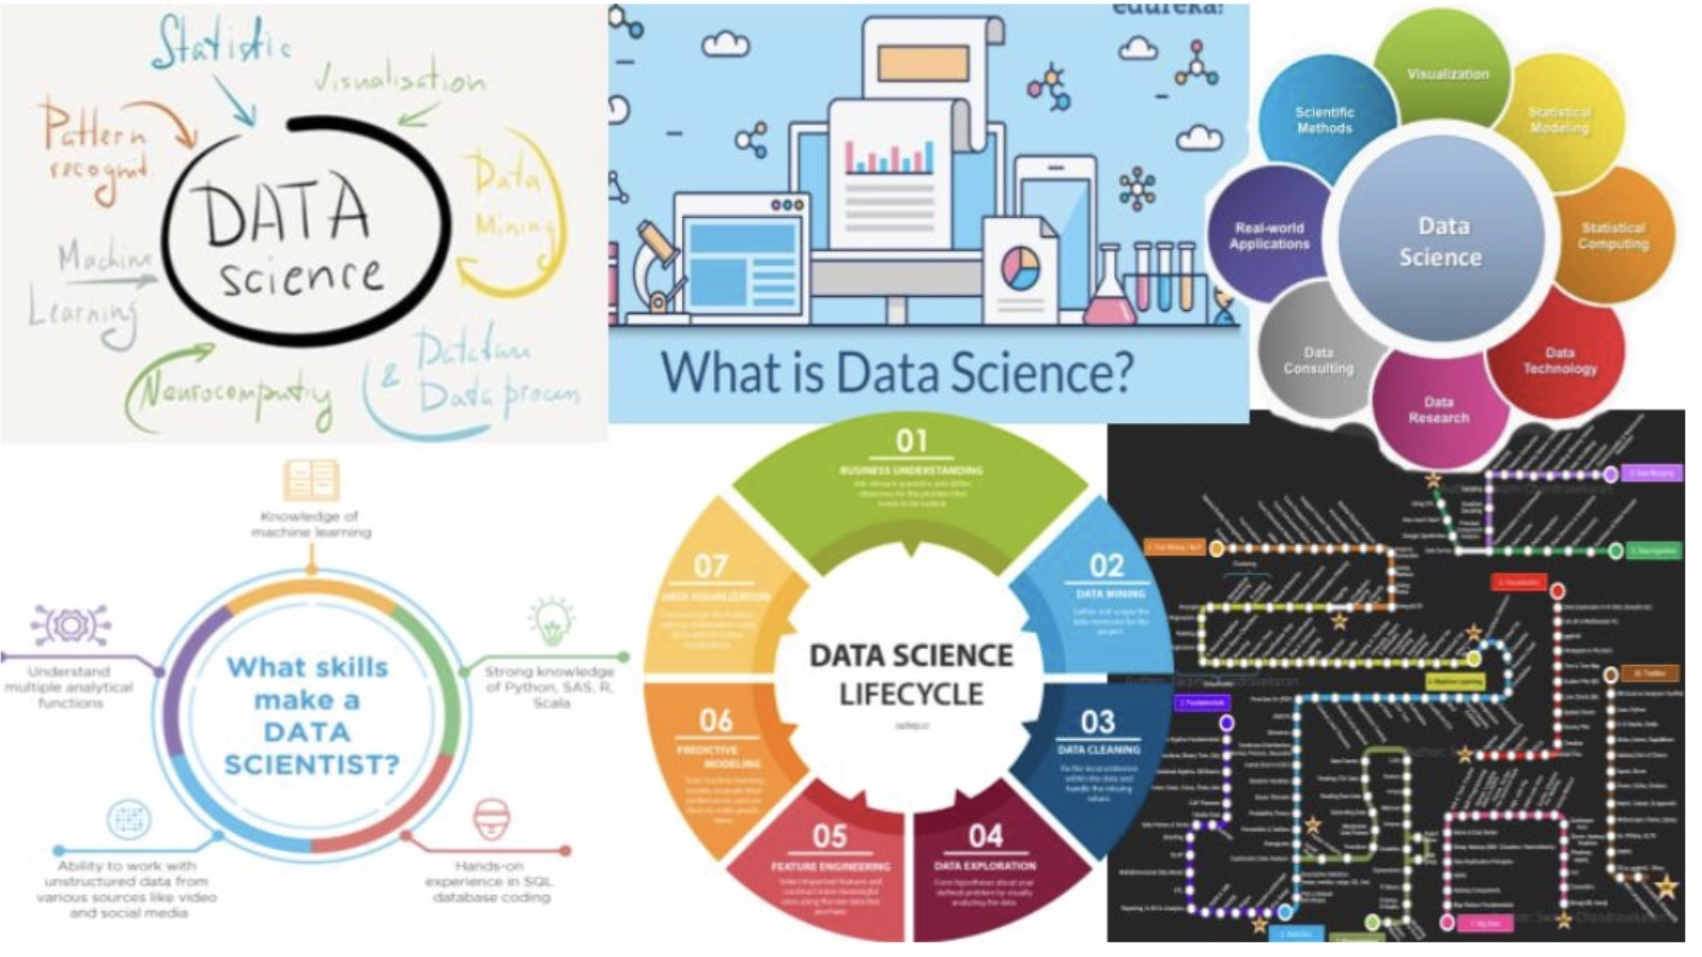
\includegraphics[width=0.6\textwidth,height=\textheight]{./images/WIDS-1.jpg}

The exact definition of Data Science can be a tad fluid. If you ask two
different data scientists, you will get two different answers. The exact
topics, skills, and outcomes could be different from person to person.
However, the general consensus is that Data Science is the practice of
using data to make decisions. This can be done in a variety of ways, but
the most common methods are through the use of statistics and machine
learning.

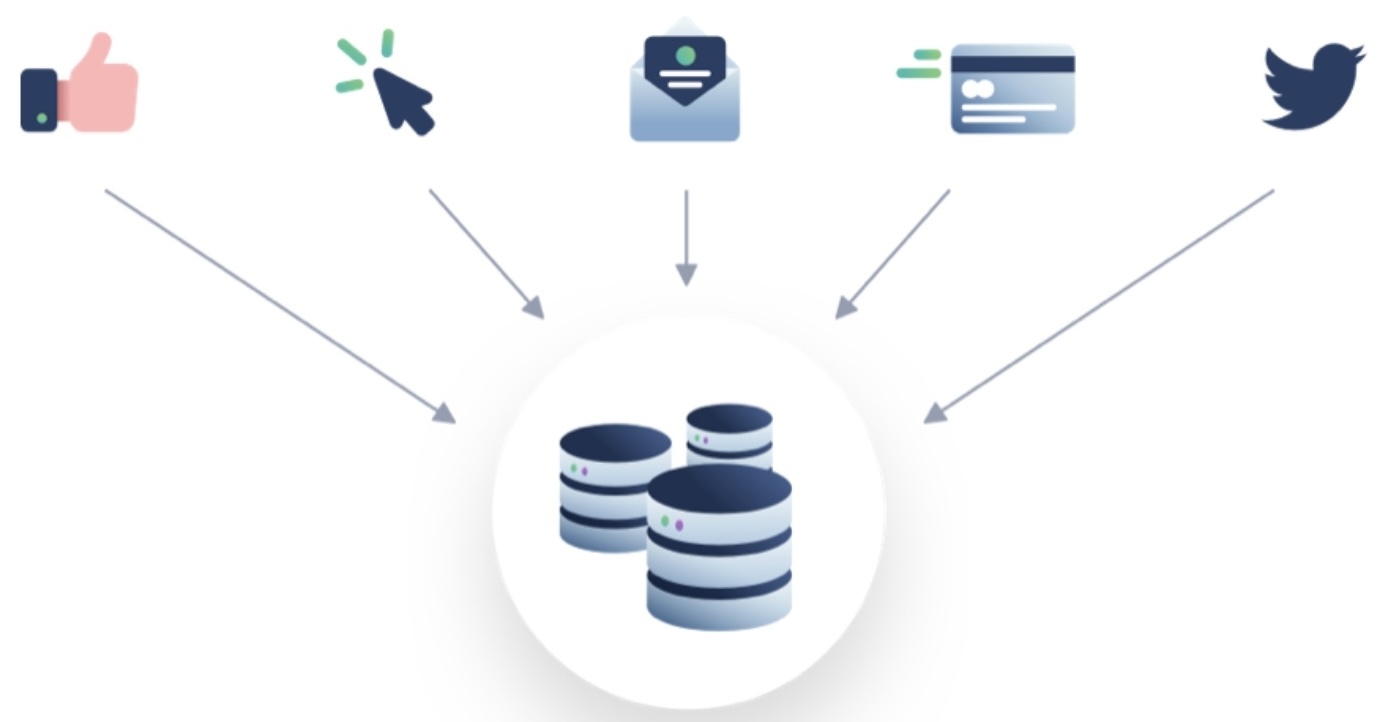
\includegraphics[width=0.6\textwidth,height=\textheight]{./images/WIDS-2.jpg}

Whether we know it or not, we are giving away tons of data every day.
When you ``like'' a social media post, use a search engine, listen to
online music, make an online purchase, or even walk around with your
phone, you are giving away data. This data is collected, stored, and
analyzed by companies to make decisions. These decisions can be as
simple as what ad to show you or as complex as what products to develop.

There are companies that collect data on everything we do. One of the
questions we are going to work through this term is how to start
analyzing this data. If we are a data scientist, what is the procedure
and timeline for analyzing data? What does the typical workflow look
like in the field of data science?

\subsection*{Step 1 : Data Collection}\label{step-1-data-collection}
\addcontentsline{toc}{subsection}{Step 1 : Data Collection}

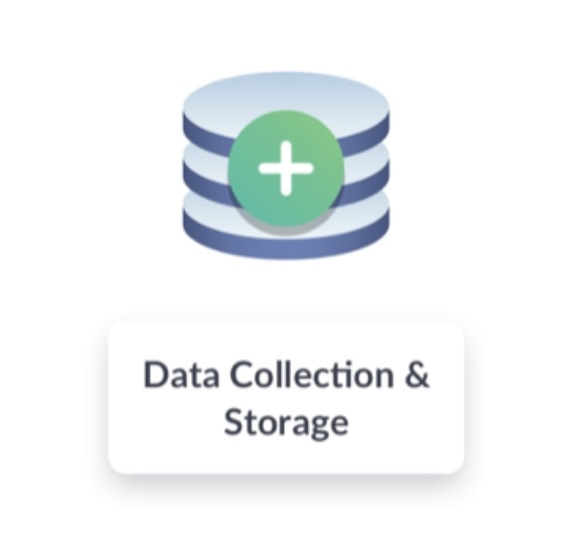
\includegraphics[width=0.25\textwidth,height=\textheight]{./images/WIDS-3.jpg}

The first step is to collect the data. As was mentioned above, this can
be done in a variety of ways. The data can be collected from a variety
of sources, some of which are going on and we don't even know it. The
data can be collected from a variety of sources, from the internet, to
social media, to smart devices, and even from the government. The data
can be collected in a variety of ways, from surveys, to interviews, to
observations, to experiments. The data can be collected in a variety of
formats, from text, to images, to audio, to video. Once the data
collection process is completed, the job of a data scientist is to take
this data and find what story it is trying to tell.

\subsection*{Step 2 : Data Preparation}\label{step-2-data-preparation}
\addcontentsline{toc}{subsection}{Step 2 : Data Preparation}

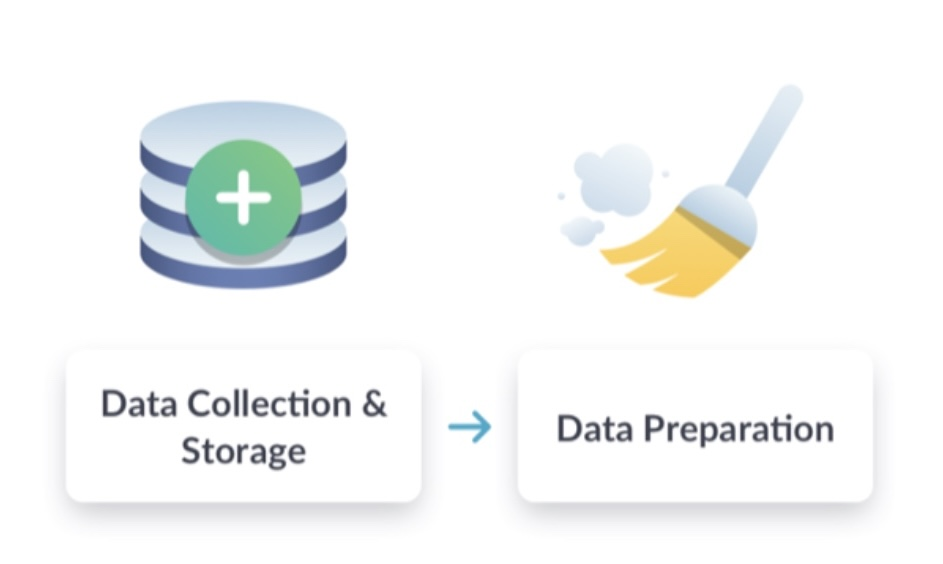
\includegraphics[width=0.4\textwidth,height=\textheight]{./images/WIDS-4.jpg}

If you talk with someone who is a data scientist, they will undoubtedly
tell you that the majority of their time is spent preparing the data.
This is because the data is often messy and needs to be cleaned up
before it can be analyzed. The data needs to bet set up in a way that
the data scientist will be able to analyze it. The data will need to be
set up so that it can be analyzed by a script. That means it needs to be
prepared (often called ``cleaned'') so that the script can read in the
data, label the variables, and start the analysis. We are trying to
structure the data set so that the script can take in the data and start
the anaylsis.

This can be done in a variety of ways, from removing missing data,
combining variables, removing duplicates, dealing with outliers, and
removing irrelevant data. Once the data is cleaned up, the job of a data
scientist is to take this data and find what story it is trying to tell.

\subsection*{Step 3 : Exploration and
Visualization}\label{step-3-exploration-and-visualization}
\addcontentsline{toc}{subsection}{Step 3 : Exploration and
Visualization}

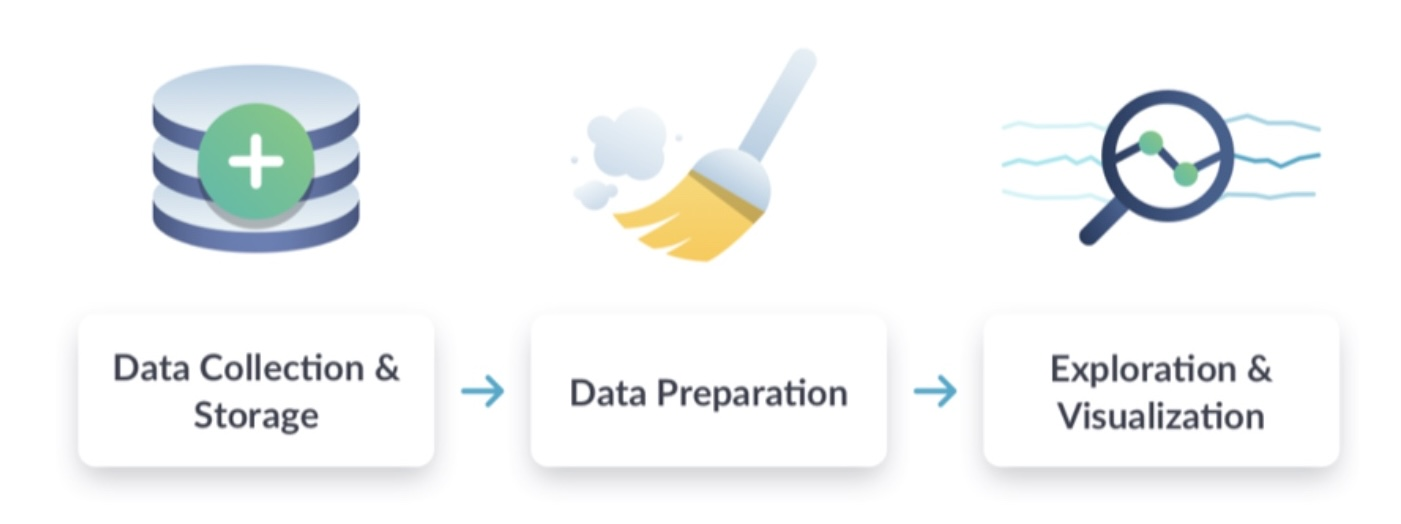
\includegraphics[width=0.55\textwidth,height=\textheight]{./images/WIDS-5.jpg}

Once the data is cleaned up, the data scientist will start to explore
the data. This can be done in a variety of ways, from looking at the
data in a table, looking at the data in a graph, or perhaps looking at
the data in a map. The data scientist will start to look at the data
with many different tools to see what story it is trying to tell.

Traditionally, the data scientist will start by looking at the data in a
table or a graph. This initial look at the data will help the data
scientist to see if there are any obvious patterns or trends in the
data. If there are, then the data scientist will start to explore these
patterns or trends in more detail.

For example, conside the story \textbf{Little Women}. The following
graph shows the cumulative number of times the names of the main
characters are used in the book.

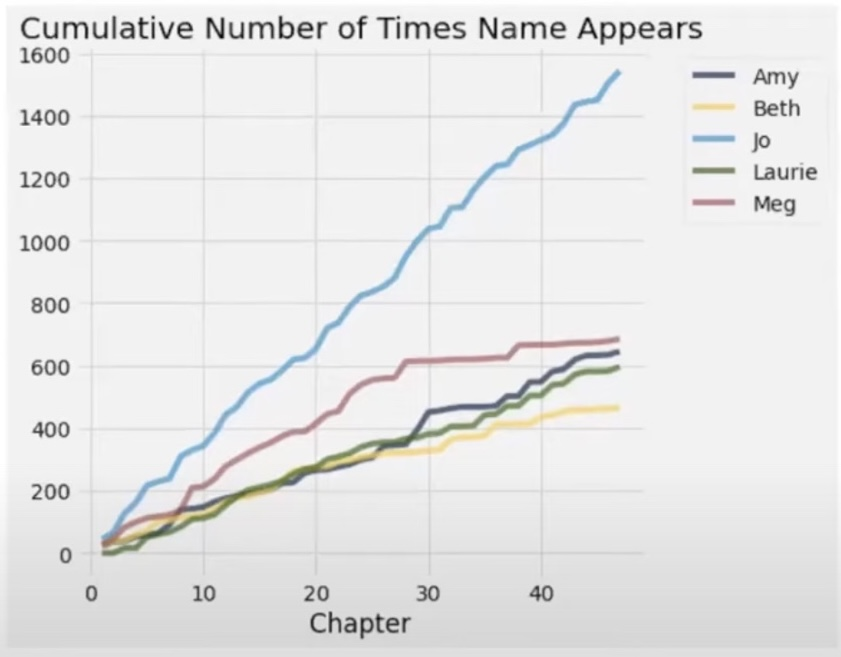
\includegraphics[width=0.4\textwidth,height=\textheight]{./images/WIDS-6.jpg}

The graph shows that the name ``Jo'' is used the most, followed by
``Meg'', ``Amy'', and ``Laurie''. If we were going to ask the question
of who the main character is in the book, the data would suggest that
the protagonist of the story is Jo. Her name appears the most in the
book, and it is not very close.While this is an interesting idea to
consider, we could also delve a little deeper at this graph. In the
story, two of the five characters listed get married to one another.
Based on this graph, can we hypothesize as to whom those two people
might be?

Based on the graph, we could hypothesize that Amy and Laurie get
married. If we examine the graph, we can see that the pattern for the
number of times Amy appears in the book is very similar to the pattern
for the number of times Laurie appears in the book starting around
chapter 35. This could suggest that the two of them are in several
scenes at the same time and when one is mentioned, then the other is
also there. Thus they are starting to spend more time together.

This proves to be true as Amy and Laurie get married in chapter 44.

\subsection*{Step 4 : Experimentation and
Prediction}\label{step-4-experimentation-and-prediction}
\addcontentsline{toc}{subsection}{Step 4 : Experimentation and
Prediction}

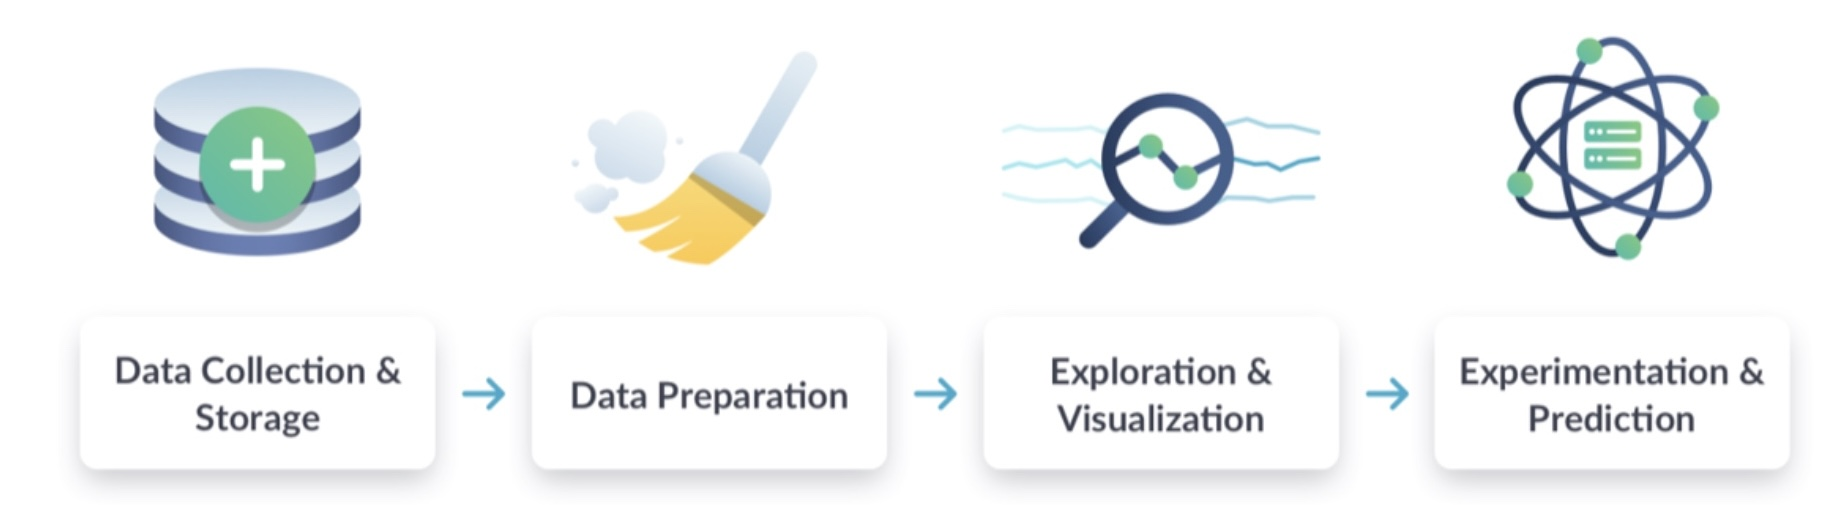
\includegraphics[width=0.7\textwidth,height=\textheight]{./images/WIDS-7.jpg}

One of the goals of a data scientist is to take data and try to figure
out what comes next.

\begin{itemize}
\tightlist
\item
  Is a stock going to rise or fall?
\item
  Is a virus going to continue to spread or die out?
\item
  Is a customer going to buy a product?
\end{itemize}

These are all questions that a data scientist will try to answer. We are
now at the stage of trying to make predictions based on the data that we
have collected, cleaned, and explored. A data scientist will make a
``Model'' that will try to predict what comes next. When we say
``model'', are really saying a mathematical equation that represents the
data set. This model will be used to make predictions about the future.
There are several ways to make a model, but this course will focus
primarily on what is know as ``linear regression''. This is a beginning
modelling technique that will introduce you to the modelling concept and
get you started on the path to making predictions.

\subsection*{Step 5 : Learning Goals}\label{step-5-learning-goals}
\addcontentsline{toc}{subsection}{Step 5 : Learning Goals}

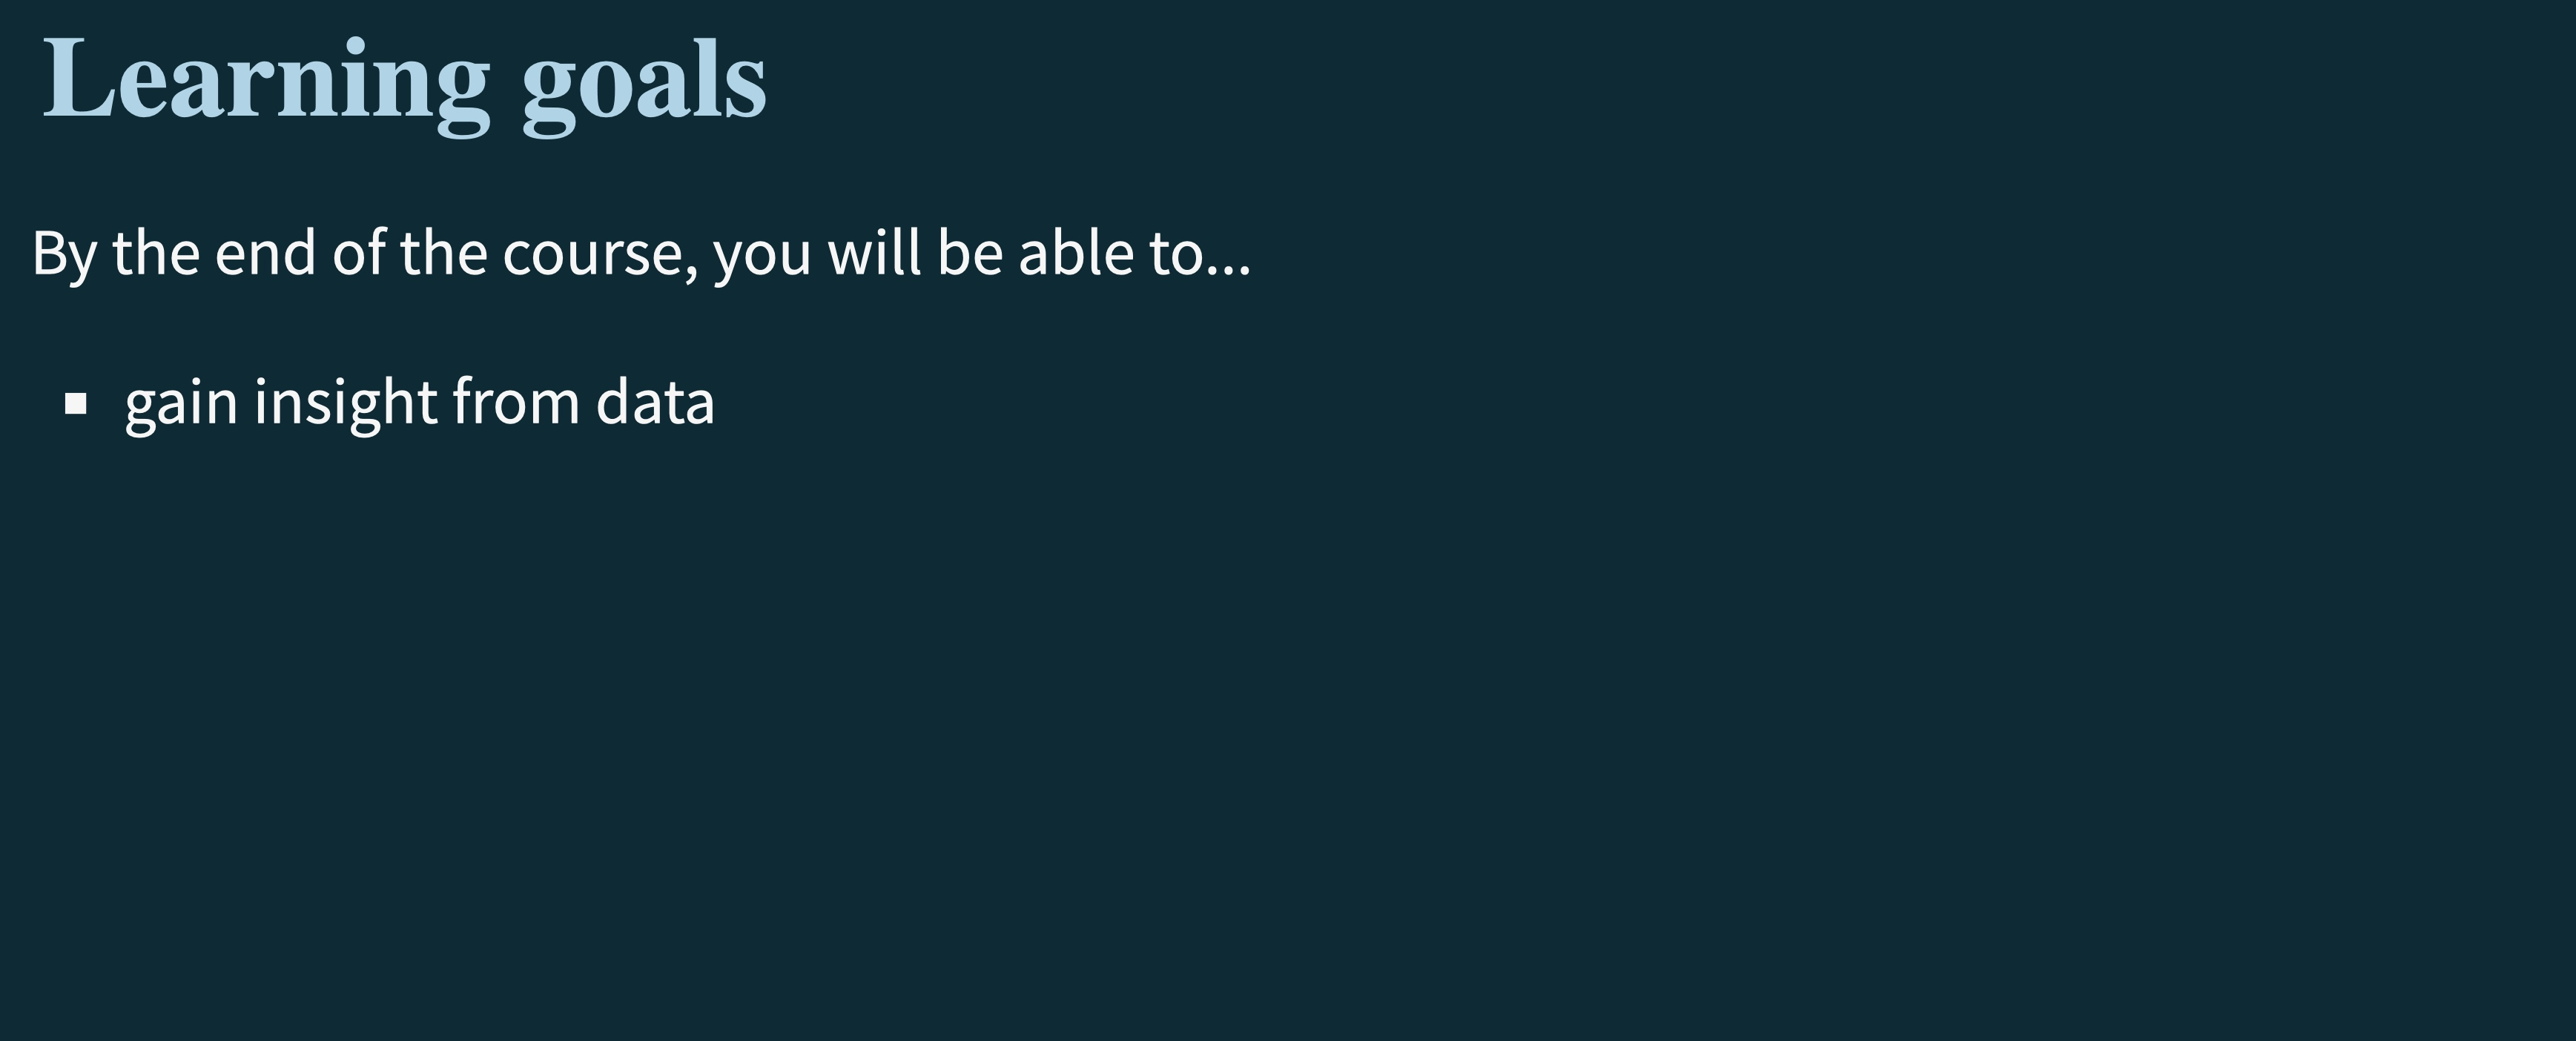
\includegraphics[width=0.6\textwidth,height=\textheight]{./images/WIDS-8.jpg}

As we walked through above, one of the main goals of this course is for
you to be able to take in a data set and find some story that it is
trying to tell. In other words, what insights can you pull out of a data
set?

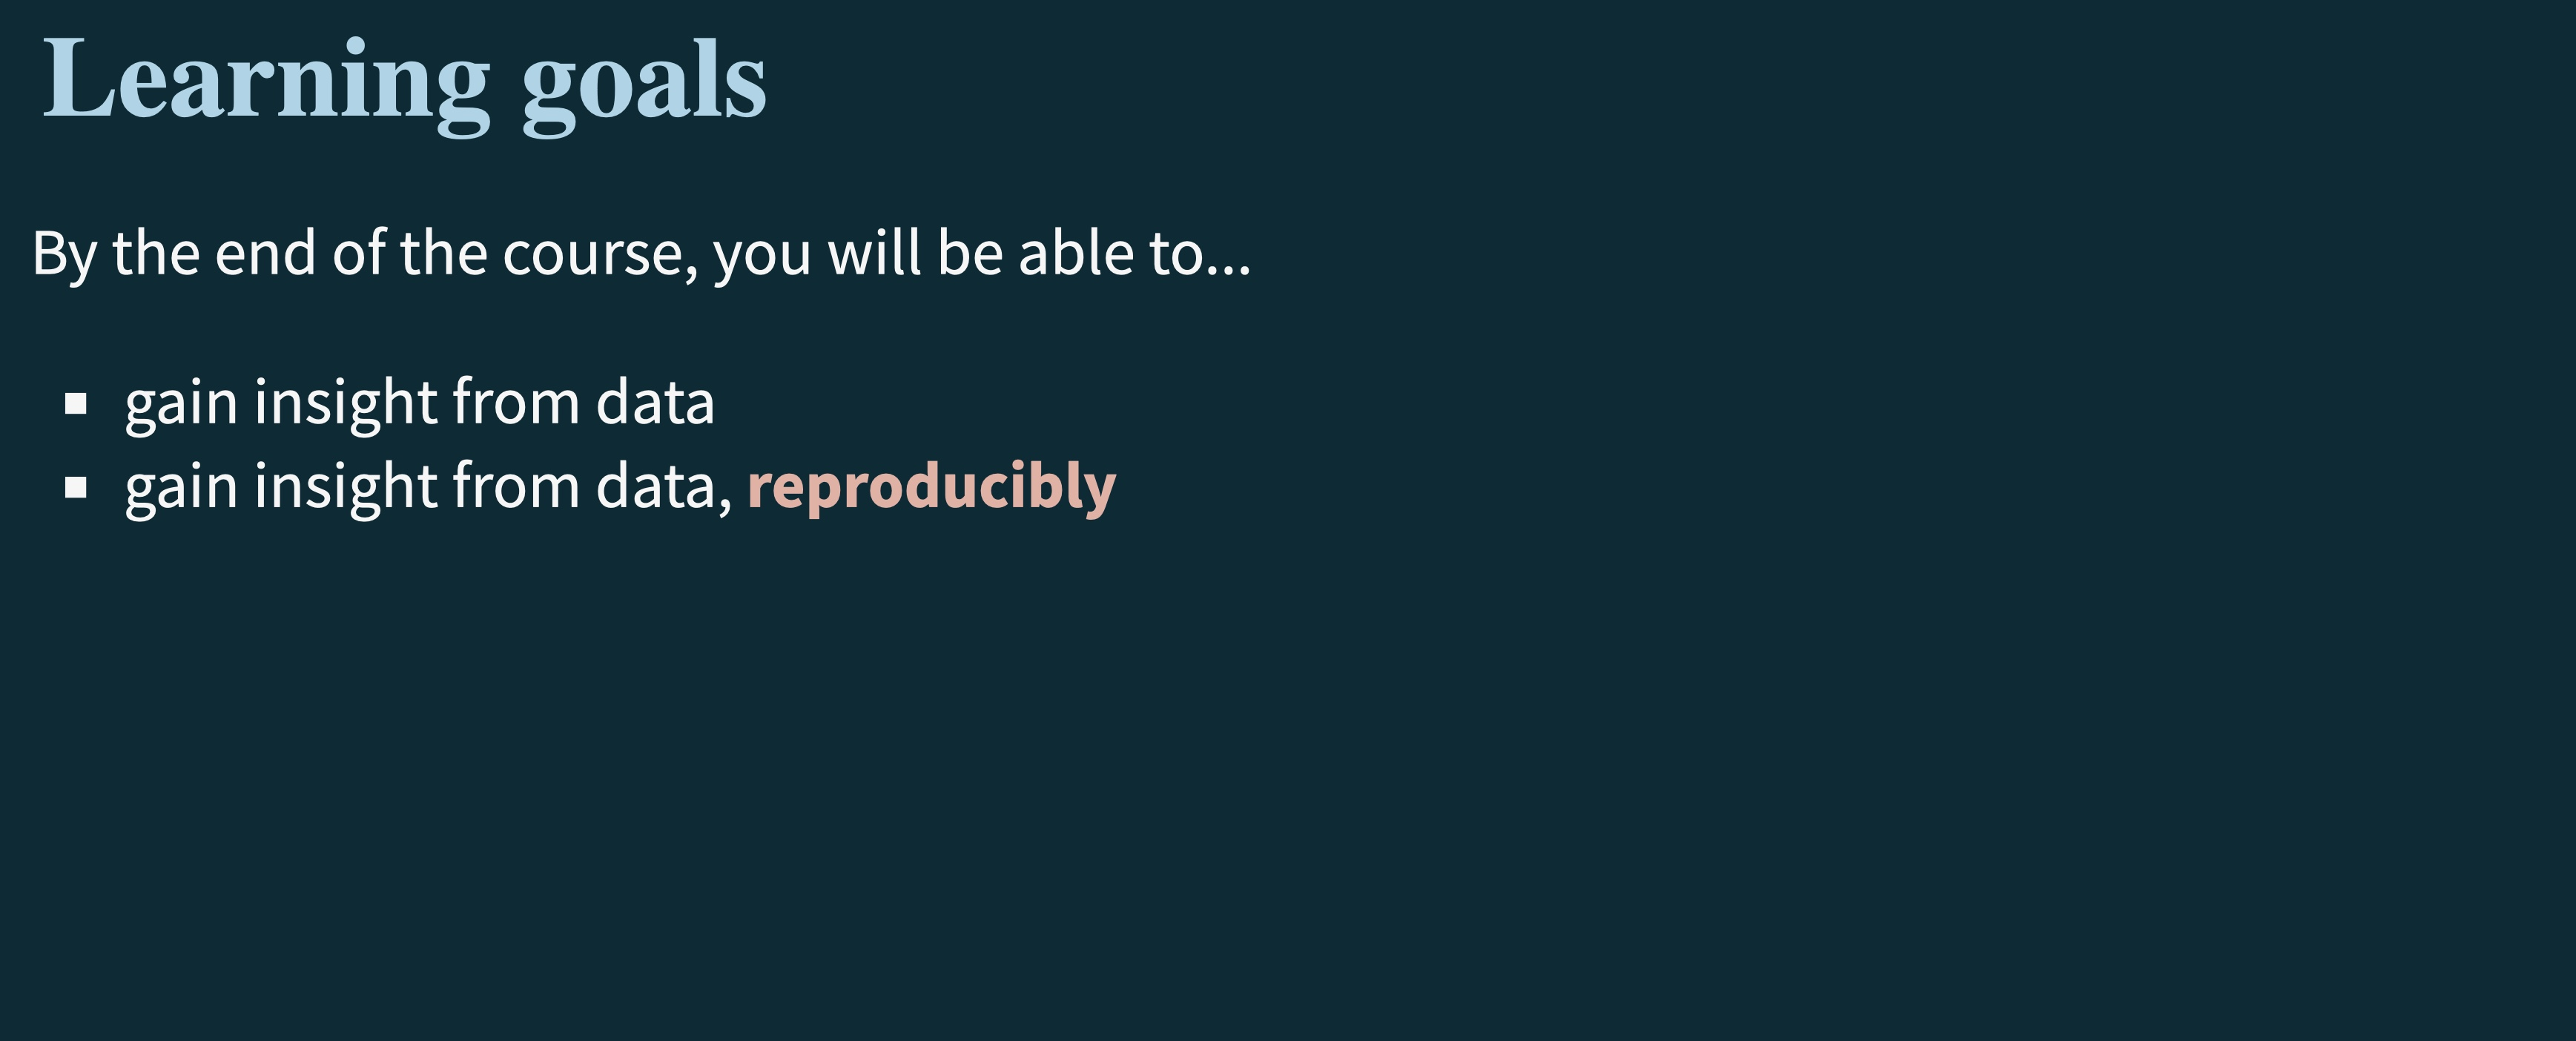
\includegraphics[width=0.6\textwidth,height=\textheight]{./images/WIDS-9.jpg}

If a data scientist, or any scientist for that matter, wants their work
to be taken seriously, then it needs to be reproducible. This means that
if you were to take the data set and the script that was used to analyze
the data, you should be able to get the same results. This is a big part
of the scientific method. If you can't reproduce the results, then the
results can not be considered reliable or valid.

For our consideration, what does it mean for work to be
``reproducible''?

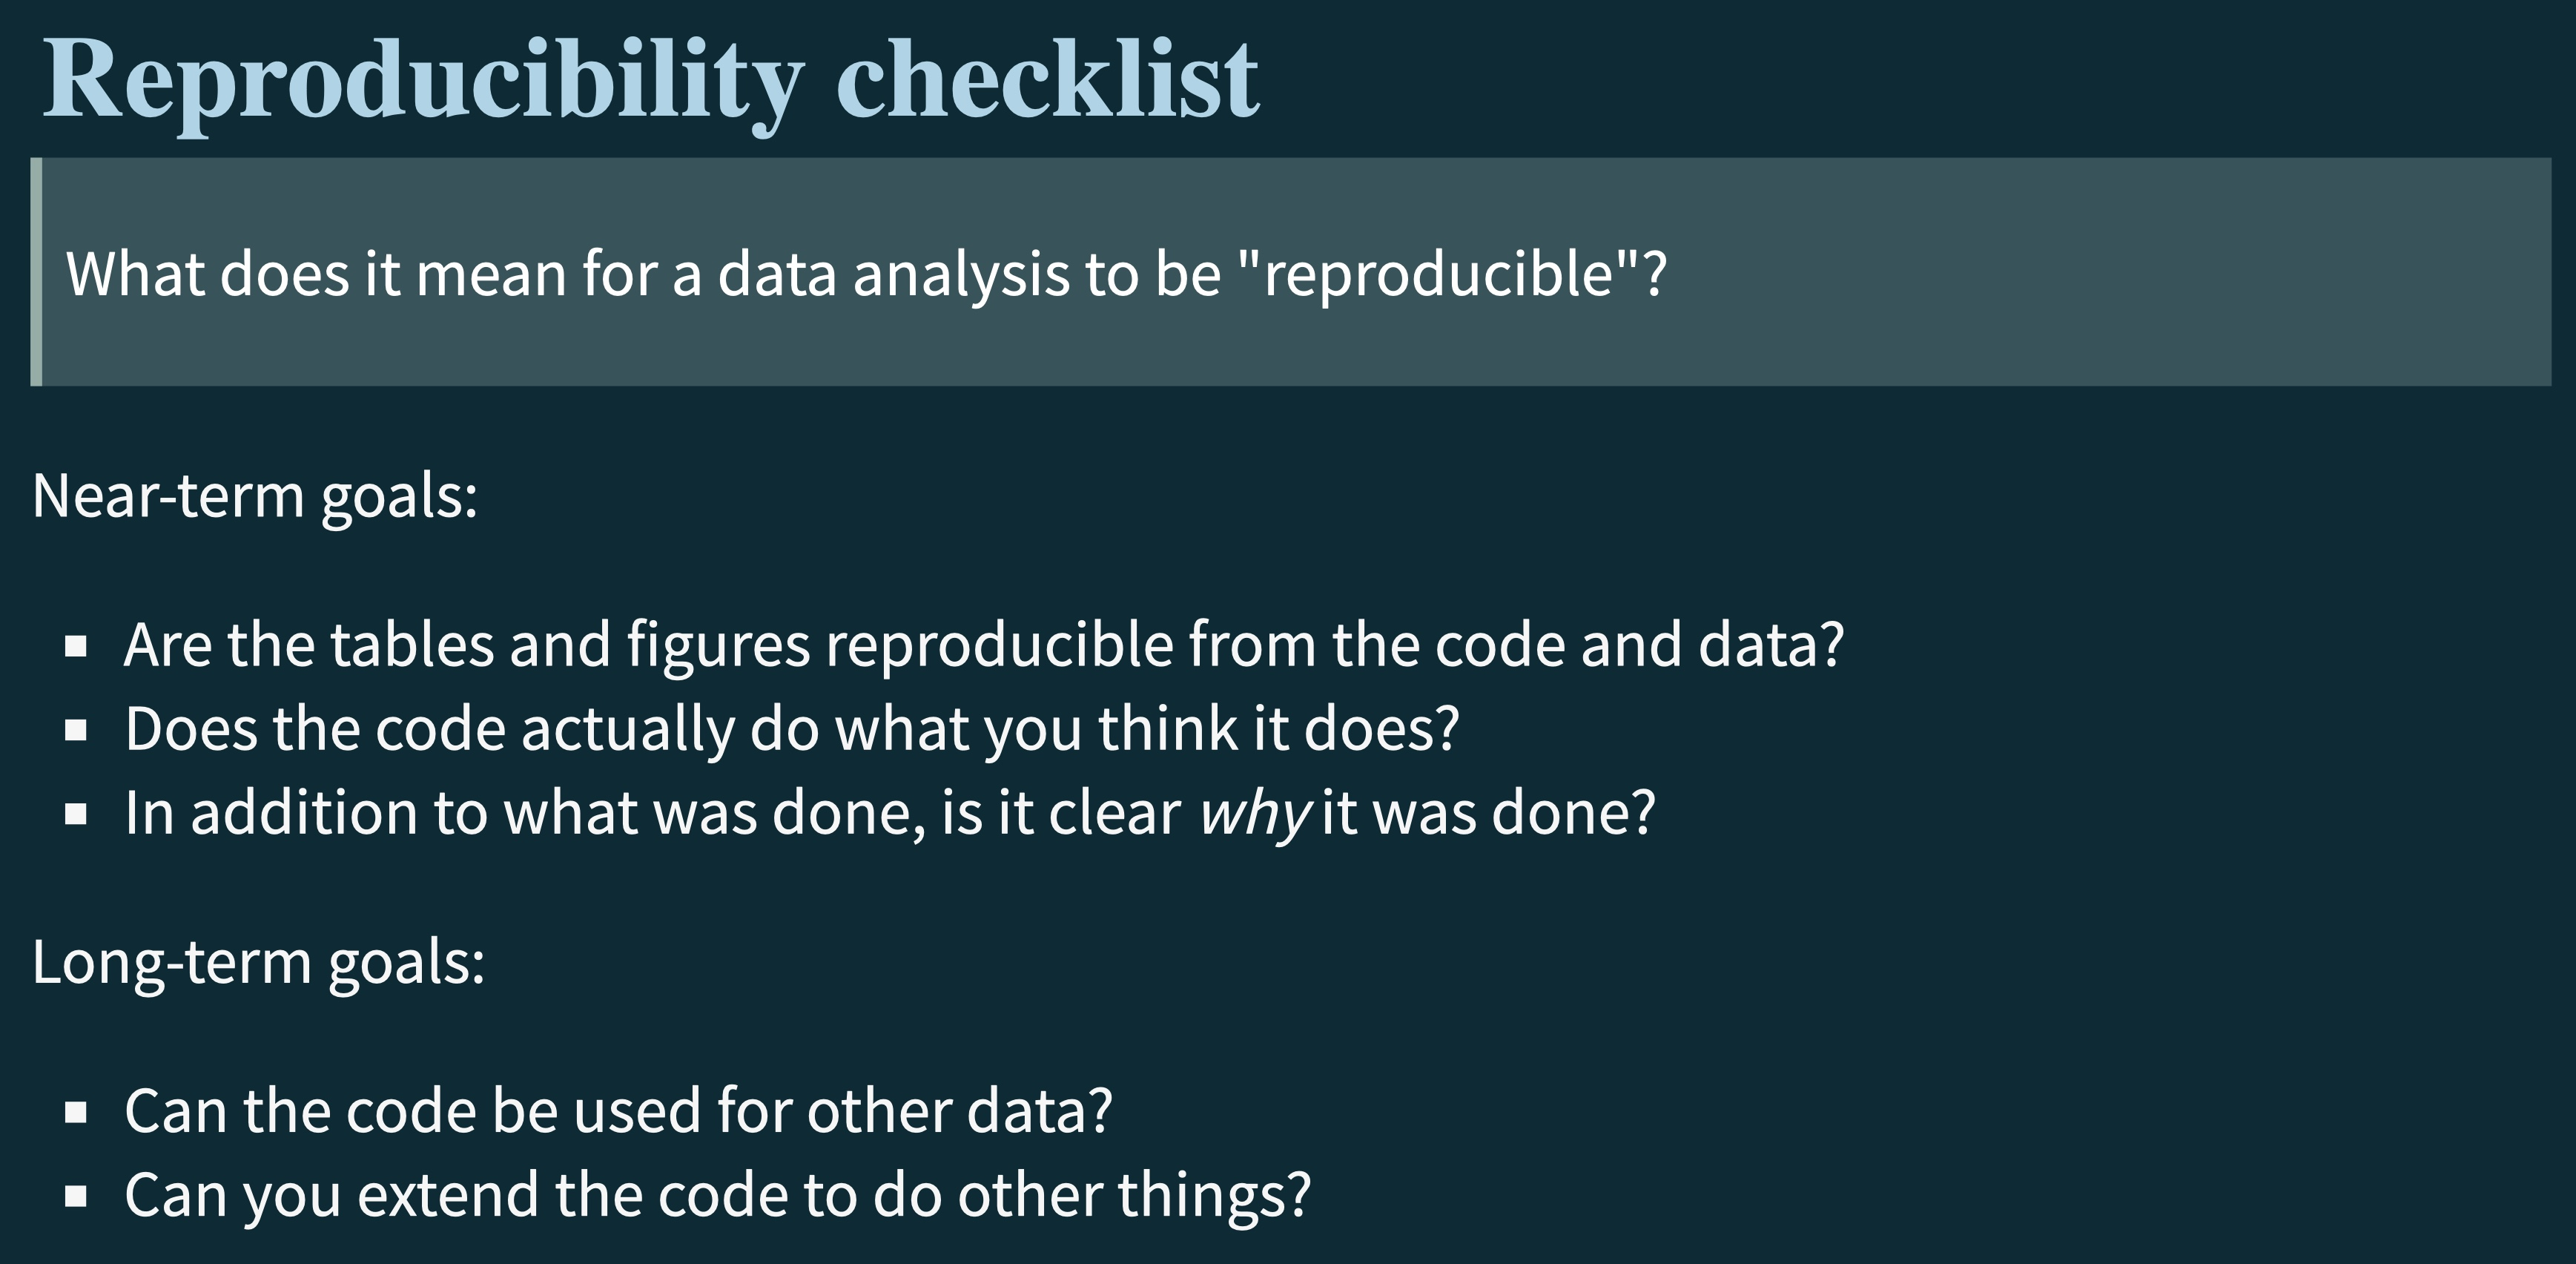
\includegraphics[width=0.6\textwidth,height=\textheight]{./images/WIDS-10.jpg}

In the graphic above, the near-term goals show you what to consider for
the project in which you are currently working. The long-term goals show
you what you should be thinking about for the future as you are working
on you current project.

You don't want to be always ``recreating the wheel''. Can you write code
that can be adapted to other data sets easily? Can you write code that
you, or someone else, could modify to find a different story in your
data set or in a different data set?

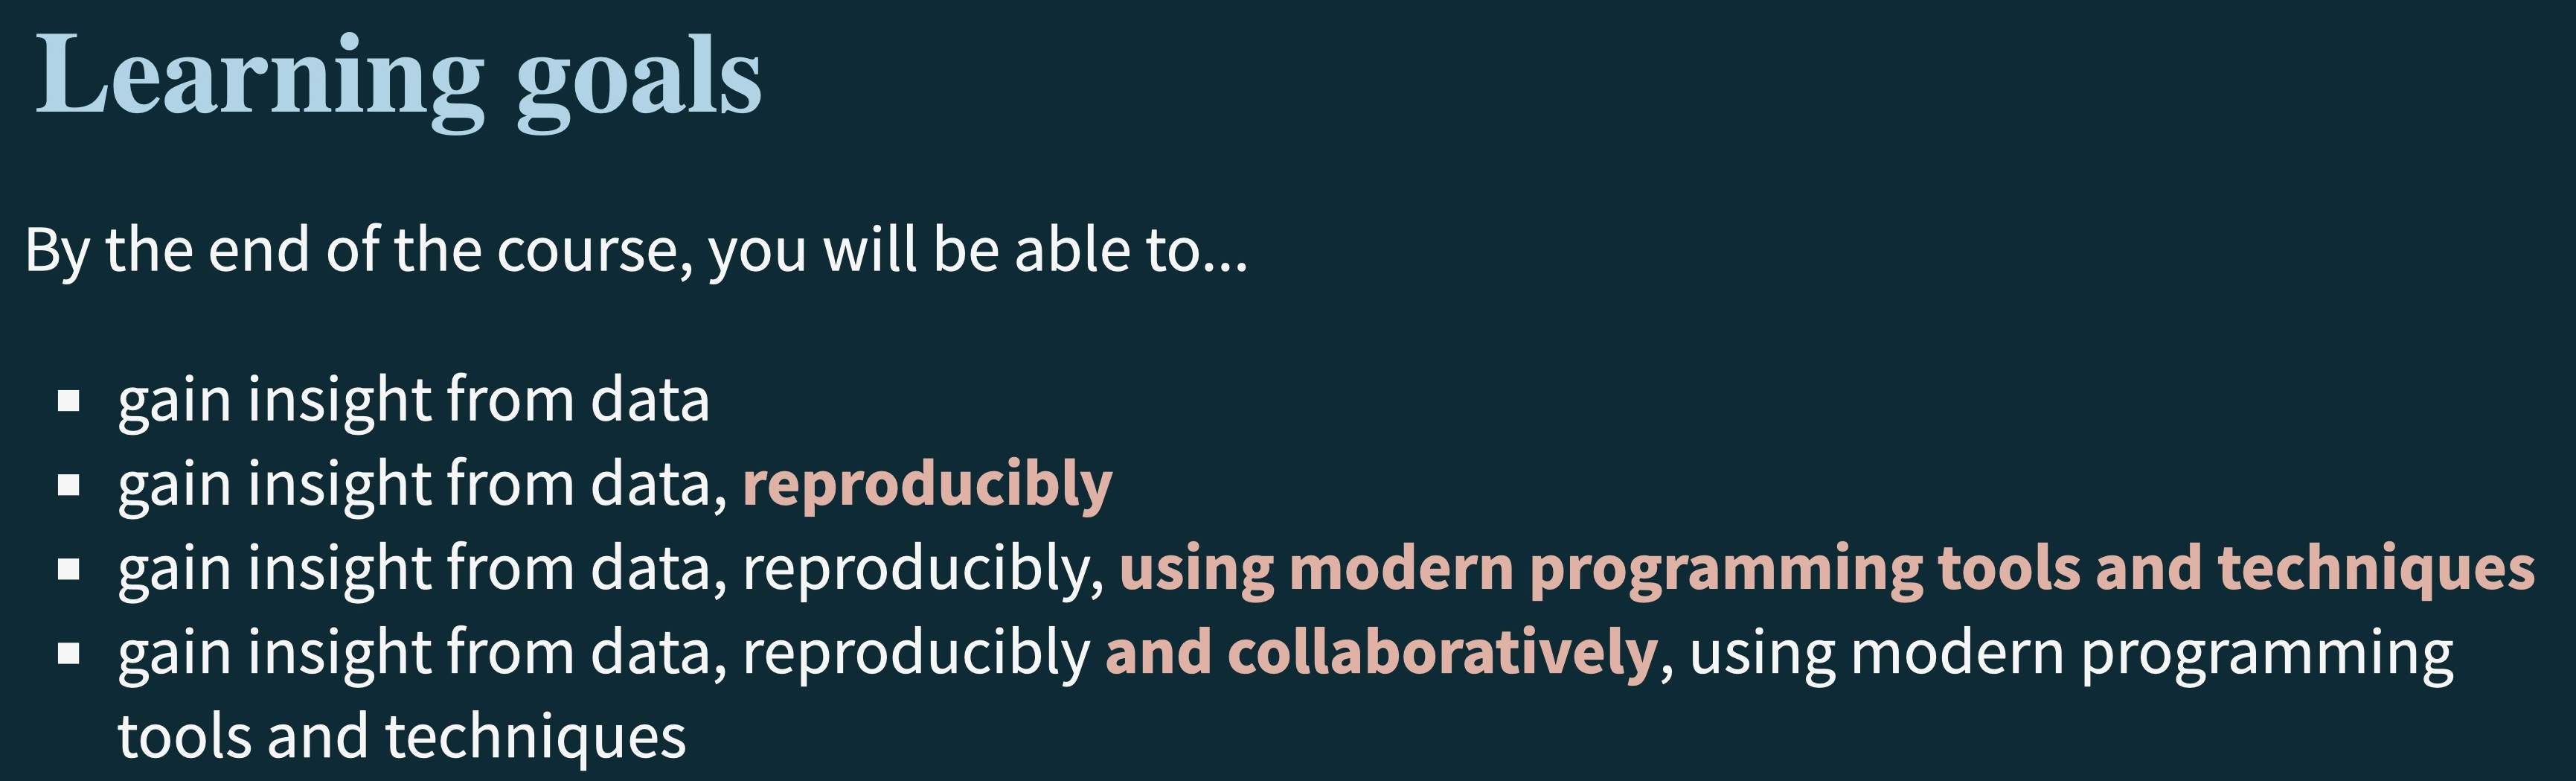
\includegraphics[width=0.6\textwidth,height=\textheight]{./images/WIDS-12.jpg}

The final two learning goals we will discuss will be working
collaboratively and using the same tools as used by data science
professionals. As you will hear from some of our data scientist guests,
they are almost always working with a group. This group analyses the
data, creates the visualizations, writes code, and finalize reports
together. Being able to work with and listen to others is a skill that
can help you become a better data scientist, better communicator, and
better team member.

When it comes to tools for data analysis, the industry standards are R
and Python. These are the two most common programming languages used by
data scientists. Academic or scientific research is often done in R,
while industry research is often done in Python. If you are going to be
a data scientist, you will need to know how to use these tools. This
course will focus on R, but do not worry if you are worried about not
using python. The two languages are very similar and if you know one,
the other is not too difficult to learn.

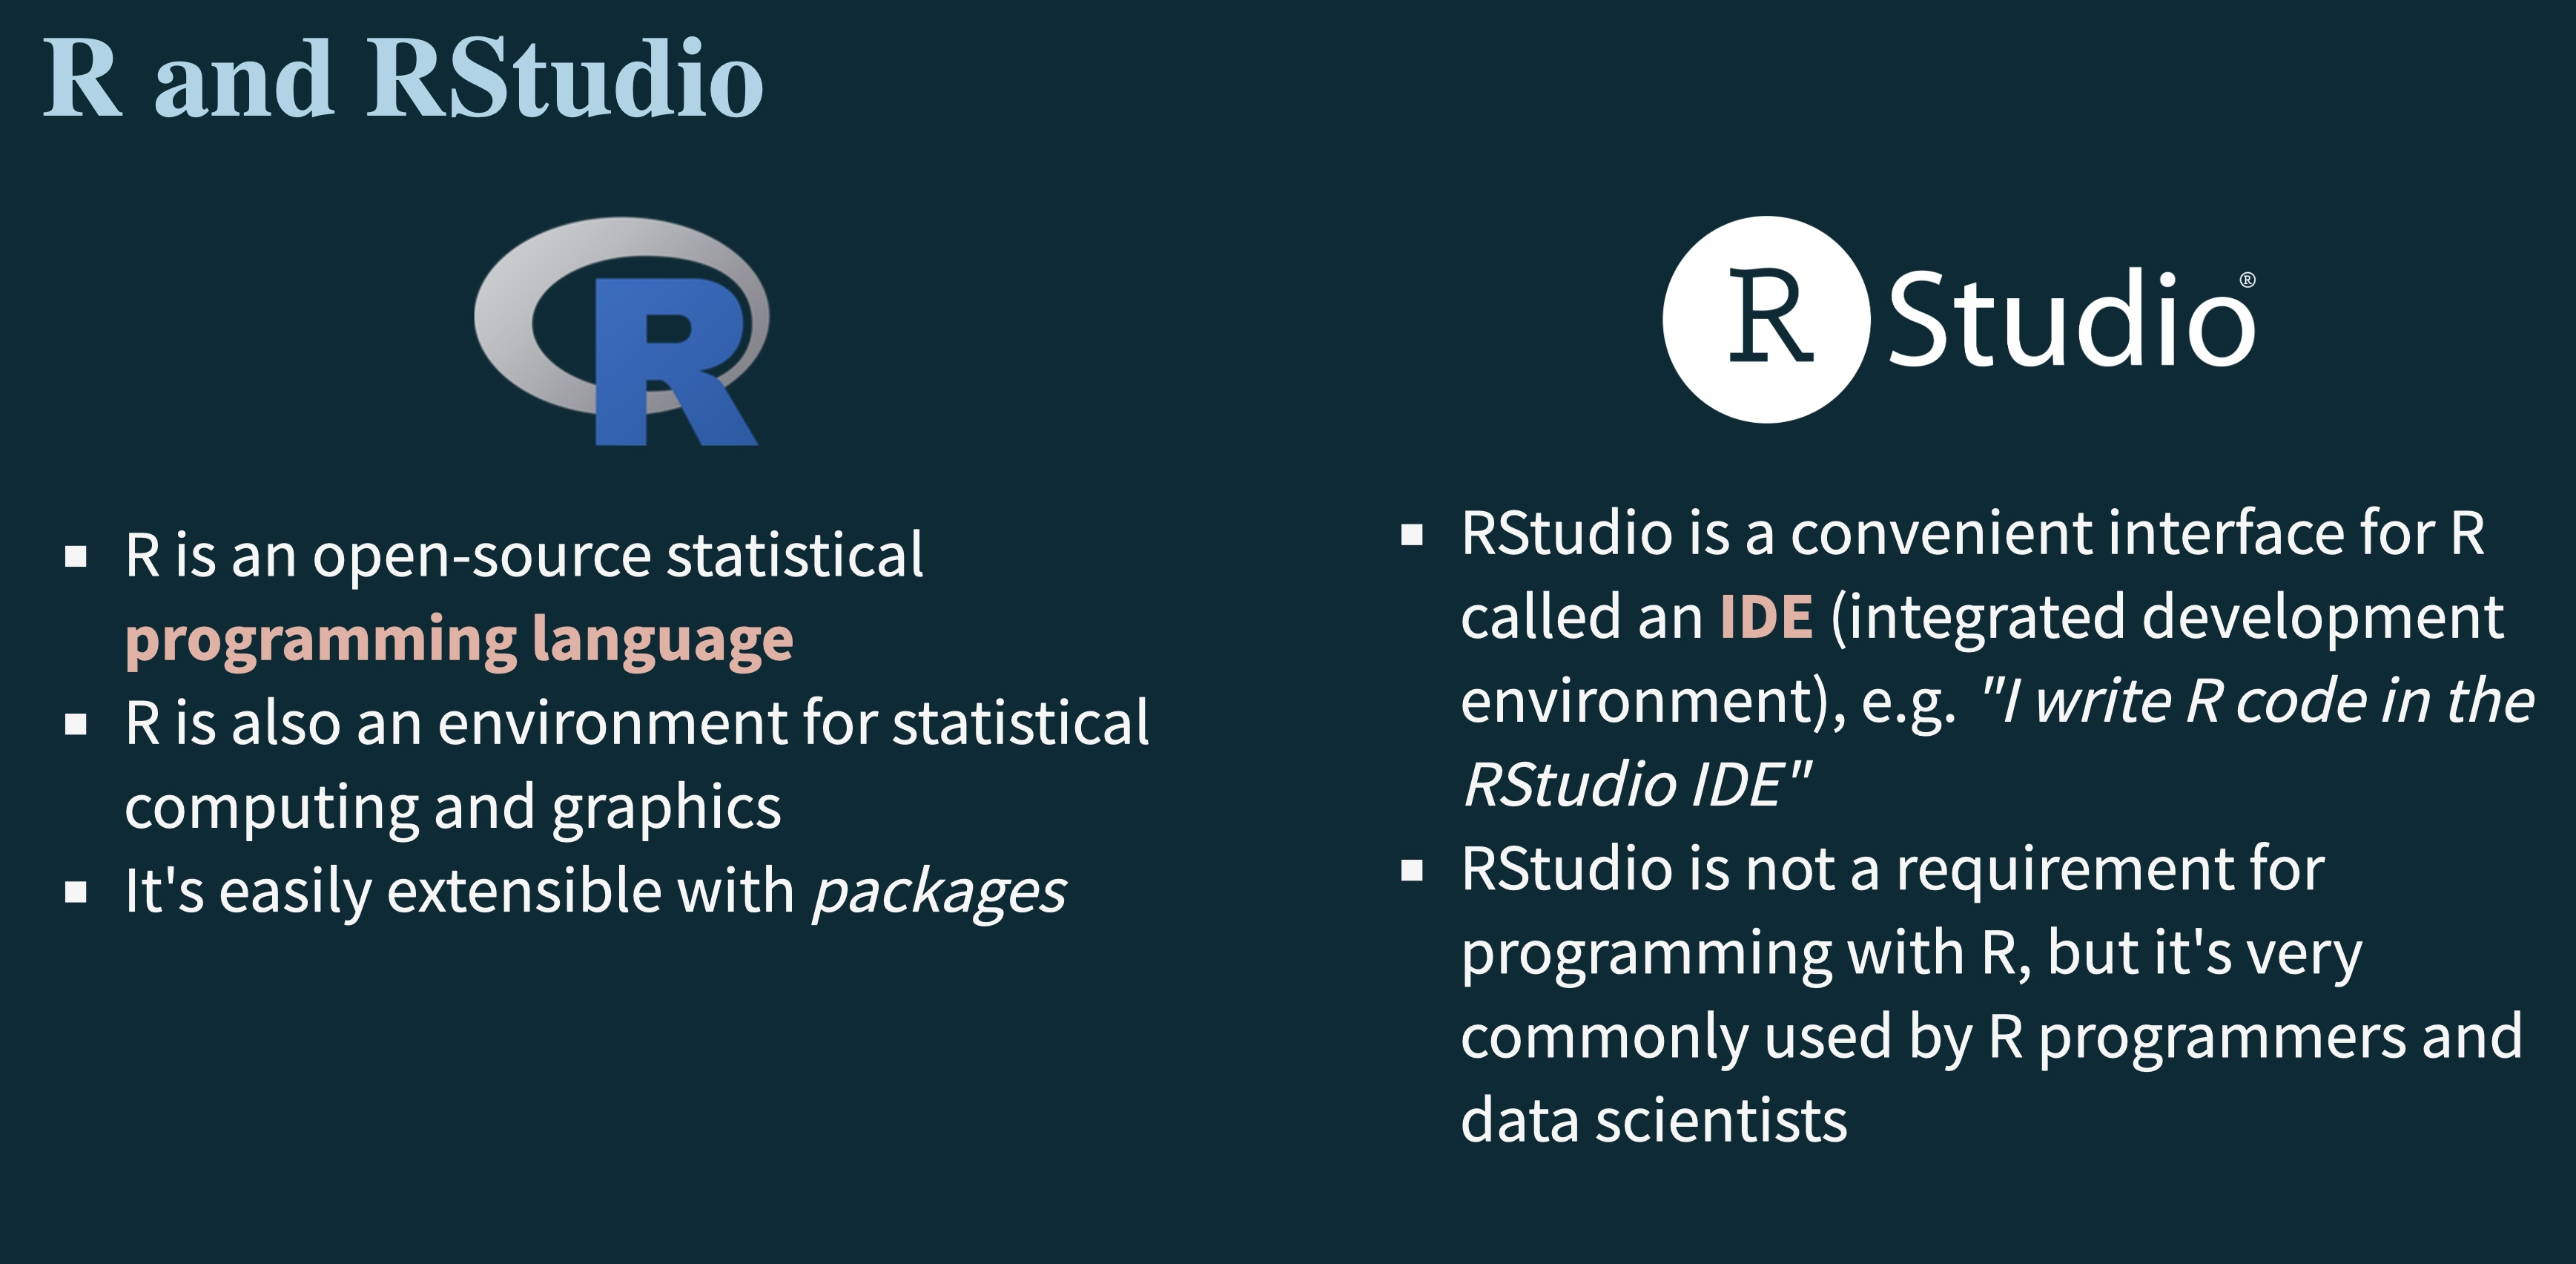
\includegraphics[width=0.6\textwidth,height=\textheight]{./images/WIDS-13.jpg}

\bookmarksetup{startatroot}

\chapter*{Qualitative and Quantitative
Variables}\label{qualitative-and-quantitative-variables}
\addcontentsline{toc}{chapter}{Qualitative and Quantitative Variables}

\markboth{Qualitative and Quantitative Variables}{Qualitative and
Quantitative Variables}

\subsection*{Qualitative Variables}\label{qualitative-variables}
\addcontentsline{toc}{subsection}{Qualitative Variables}

Qualitative variables are variables that are not numerical. They are
categorical variables that can be divided into groups, which is why they
are often referred to as \textbf{categorical variables}. You have
probably encountered these when you have filled out an application for
employment. You may have had to check boxes regarding ethnicity, level
of education or gender. These are all examples of qualitative variables.
We can also break them down into two different types of qualitative
variables, \textbf{nominal} and \textbf{ordinal} variables.

\textbf{Nominal} variables are variables that have no order. For
example,

\begin{itemize}
\tightlist
\item
  Hair or Eye Color
\item
  Religious Affiliation
\item
  Gender
\item
  Marital Status
\item
  Political Affiliation
\end{itemize}

Even though these are not numerical variables, we could still create
some numerical structures based off of nominal variables that will help
us understand the data. For example, assume we took a survey of 200
Transylvania University students about their favorite sport to watch and
that 97 said Football, 62 said Basketball, and 41 said Others. Based on
this data, we could create a bar graph to show the distribution of
favorite sports to watch. (Don't worry about knowing these commands yet.
We will get to these commands later in the course.)

We need to first create the data frame for the variable :

\begin{Shaded}
\begin{Highlighting}[]
\CommentTok{\# Create a dataframe. We will first create a vector that has the names}
\CommentTok{\# of the sports and another vector that has the number of students that}
\CommentTok{\# like each sport.}

\NormalTok{sports }\OtherTok{\textless{}{-}} \FunctionTok{c}\NormalTok{(}\StringTok{"Football"}\NormalTok{, }\StringTok{"Basketball"}\NormalTok{, }\StringTok{"Others"}\NormalTok{)}

\NormalTok{students }\OtherTok{\textless{}{-}} \FunctionTok{c}\NormalTok{(}\DecValTok{97}\NormalTok{, }\DecValTok{62}\NormalTok{, }\DecValTok{41}\NormalTok{)}

\CommentTok{\# We will then put them together into a data frame.}

\NormalTok{df }\OtherTok{\textless{}{-}} \FunctionTok{data.frame}\NormalTok{(sports, students)}

\CommentTok{\# And print out the data frame to make sure it looks correct.}

\NormalTok{df}
\end{Highlighting}
\end{Shaded}

\begin{verbatim}
      sports students
1   Football       97
2 Basketball       62
3     Others       41
\end{verbatim}

Even though this data is nominal, we could also create a bar graph to
show the distribution of favorite sports to watch.

\begin{Shaded}
\begin{Highlighting}[]
\CommentTok{\# Create a bar graph using ggplot}

\CommentTok{\# We need to load the ggplot library.}

\FunctionTok{library}\NormalTok{(ggplot2)}

\CommentTok{\# We can now create the bar graph.}

\FunctionTok{ggplot}\NormalTok{(df, }\FunctionTok{aes}\NormalTok{(}\AttributeTok{x =}\NormalTok{ sports, }\AttributeTok{y =}\NormalTok{ students)) }\SpecialCharTok{+} 
  \FunctionTok{geom\_bar}\NormalTok{(}\AttributeTok{stat =} \StringTok{"identity"}\NormalTok{, }\AttributeTok{fill =} \StringTok{"darkred"}\NormalTok{) }\SpecialCharTok{+}
  \FunctionTok{geom\_text}\NormalTok{(}\FunctionTok{aes}\NormalTok{(}\AttributeTok{label =}\NormalTok{ students), }\AttributeTok{vjust =} \SpecialCharTok{{-}}\FloatTok{0.3}\NormalTok{, }\AttributeTok{color =} \StringTok{"black"}\NormalTok{) }\SpecialCharTok{+}
  \FunctionTok{labs}\NormalTok{(}\AttributeTok{title =} \StringTok{"Transy Students Favorite Sports to Watch"}\NormalTok{, }
       \AttributeTok{x =} \StringTok{"Sports"}\NormalTok{, }\AttributeTok{y =} \StringTok{"Number of Students"}\NormalTok{)}
\end{Highlighting}
\end{Shaded}

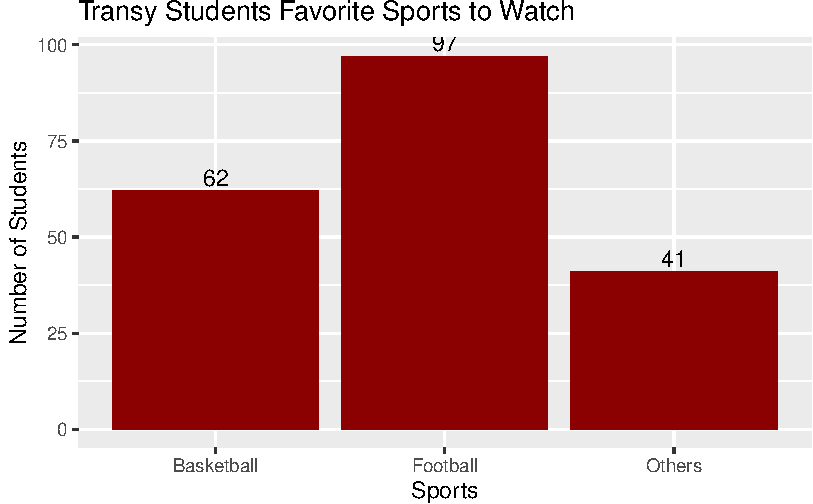
\includegraphics{Qualitative_and_Quantitative_Variables_files/figure-pdf/unnamed-chunk-2-1.pdf}

\textbf{Ordinal} variables are qualitative variables that have an order.
For example, the variable ``education'' is an ordinal variable because
there is an order to the levels of education. They could include the
following:

\begin{itemize}
\tightlist
\item
  educational level (high school, bachelor's, master's)
\item
  clothing size (small, medium, large)
\item
  customer satisfaction rating (dissatisfied, neutral, satisfied)
\item
  pain level (mild, moderate, severe)
\item
  socioeconomic status (low, middle, high).
\end{itemize}

Ordinal variables are often treated as categorical variables, but if it
makes sense, then they can also be treated as numerical variables. What
we would need to do is to assign each of the variables a numerical value
that corresponds to the level of the variable.

We could perform the same commands we did above, but by adding numerical
values to the variables, we might be able to do other meaningful
analysis. For instance, if we were to assign a numerical value to the
levels of education (high school = 1, bachelor's = 2, master's = 3), we
could do something such as calculating the mean level of education for a
group of people.

Notice that we could always add numerical values to qualitative
variables, but it doesn't always make sense to do so. Consider the hair
color example. We could assign value to different outcomes (black = 1,
brown = 2, blonde = 3, etc.) but what would we then do with this data?
It doesn't make sense to calculate the mean hair color of a group of
people, especially if the way you label the numbers to variables is
different from how I would label them. What would the averages describe?
This is why we will call a qualitative variable a \textbf{nominal}
variable if it doesn't make sense to assign numerical values to the
variable, and we will call it an \textbf{ordinal} variable if it does
make sense to assign numerical values to the variable.

\subsection*{Quantitative Variables}\label{quantitative-variables}
\addcontentsline{toc}{subsection}{Quantitative Variables}

Quantitative variables are numerical variables. Just like the
qualitative variables above, we can be divide quantitative variables
into two different categories, \textbf{discrete} and \textbf{continuous}
variables.

\textbf{Discrete} variables are variables that can only take on certain
values, are countable, and are indivisible. For example, the number of
students in a class is a discrete variable because it can only take on
certain values (1, 2, 3, 4, etc.). Clearly you can't have a class with
12.5 students. The number of siblings a person has is also a discrete
variable because it can only take on certain values (0, 1, 2, 3, etc.).
The number of cars a person owns is a discrete variable because it can
only take on certain values (0, 1, 2, 3, etc.). Similarly, you couldn't
have 2.3 siblings or 4.8 cars.

When it comes to the analysis of discrete data, the tools we will use
are similar to the ones we used for qualitative data. We will use bar
graphs, tables, pie charts, and other visualizations to help us
understand the data.

\textbf{Continuous} variables are variables that can take on any value
in a certain range. A continuous variable takes on an infinite number of
possible values within a given range. For example, the height of a
person is a continuous variable because it can take on any value (5.2,
5.317, 5.4611, etc.). The weight of a person is a continuous variable
because it can take on any value (120, 121.3, 122, etc.). The amount of
time it takes to complete a task is a continuous variable because it can
take on any value (5.2, 5.3, 5.4, etc.).

Because the possible values for a continuous variable are infinite, we
measure continuous variables (rather than count), often using a
measuring device like a ruler or stopwatch. Continuous variables include
all the fractional or decimal values within a range.

Sometimes we treat continuous variables as if they were discrete. Age is
an excellent example of this. If you know a person's time of birth, you
could measure their age precisely up to the second or even millisecond
if you wanted to. In this sense, age is a continuous variable. However,
we don't usually care about a person's exact age. Instead, we treat age
as a discrete variable and count age in years.

Analyzing continuous variables in R primarily involves calculating
descriptive statistics like mean, median, standard deviation, and
visualizing the data distribution using plots like histograms, density
plots, and boxplots, allowing you to understand the central tendency,
spread, and potential skewness of the data; you can also explore
relationships between continuous variables using scatterplots and
calculate correlation coefficients to assess their linear association

Let's create a data set of continuous variables and analyze it. We will
pick 1000 values from 0 to 10.

\begin{Shaded}
\begin{Highlighting}[]
\CommentTok{\# We shall "set the seed" for randomization. This allows us to get the same}
\CommentTok{\# values everytime we run these commands. Without this, the results would be}
\CommentTok{\# different each time.}

\FunctionTok{set.seed}\NormalTok{(}\DecValTok{1123}\NormalTok{)}

\CommentTok{\# Generate 1000 random values between 0 and 10 and store them in the }
\CommentTok{\# variable \textquotesingle{}data\_example\textquotesingle{}}

\NormalTok{df }\OtherTok{\textless{}{-}} \FunctionTok{runif}\NormalTok{(}\DecValTok{1000}\NormalTok{, }\AttributeTok{min =} \DecValTok{0}\NormalTok{, }\AttributeTok{max =} \DecValTok{10}\NormalTok{) }

\CommentTok{\# Here are the first six values in the data set, using the head( ) command :}

\FunctionTok{head}\NormalTok{(df)}
\end{Highlighting}
\end{Shaded}

\begin{verbatim}
[1] 7.595128 8.609249 8.658766 5.518078 8.264048 1.620436
\end{verbatim}

We could now carry out some analysis such as calculating the mean,
median, and standard deviation of the data set. We could also create a
histogram to show the distribution of the data. These are the types of
analysis we will be doing using continuous variables.

\begin{Shaded}
\begin{Highlighting}[]
\CommentTok{\# Calculate the mean of the data set}

\FunctionTok{mean}\NormalTok{(df)}
\end{Highlighting}
\end{Shaded}

\begin{verbatim}
[1] 4.932104
\end{verbatim}

\begin{Shaded}
\begin{Highlighting}[]
\CommentTok{\# Calculate the median of the data set}

\FunctionTok{median}\NormalTok{(df)}
\end{Highlighting}
\end{Shaded}

\begin{verbatim}
[1] 4.919963
\end{verbatim}

\begin{Shaded}
\begin{Highlighting}[]
\CommentTok{\# create a histogram with 10 bars (bins) for the data set}

\FunctionTok{ggplot}\NormalTok{(}\AttributeTok{data =} \FunctionTok{data.frame}\NormalTok{(df), }\FunctionTok{aes}\NormalTok{(}\AttributeTok{x =}\NormalTok{ df, }\AttributeTok{y =} \FunctionTok{after\_stat}\NormalTok{(density))) }\SpecialCharTok{+}
  \FunctionTok{geom\_histogram}\NormalTok{(}\AttributeTok{bins =} \DecValTok{10}\NormalTok{, }\AttributeTok{binwidth =} \DecValTok{1}\NormalTok{, }\AttributeTok{center=}\FloatTok{0.5}\NormalTok{, }\AttributeTok{fill =} \StringTok{"darkred"}\NormalTok{, }\AttributeTok{color =} \StringTok{"black"}\NormalTok{) }\SpecialCharTok{+}
  \FunctionTok{scale\_x\_continuous}\NormalTok{(}\AttributeTok{breaks =} \FunctionTok{seq}\NormalTok{(}\DecValTok{0}\NormalTok{, }\DecValTok{10}\NormalTok{, }\AttributeTok{by =} \DecValTok{1}\NormalTok{), }\AttributeTok{limits =} \FunctionTok{c}\NormalTok{(}\DecValTok{0}\NormalTok{,}\DecValTok{10}\NormalTok{))}\SpecialCharTok{+}
    \FunctionTok{stat\_bin}\NormalTok{(}\AttributeTok{geom =} \StringTok{"text"}\NormalTok{, }\FunctionTok{aes}\NormalTok{(}\AttributeTok{label =} \FunctionTok{round}\NormalTok{(}\FunctionTok{after\_stat}\NormalTok{(density),}\DecValTok{3}\NormalTok{), }\AttributeTok{y=}\FloatTok{0.5}\SpecialCharTok{*}\FunctionTok{after\_stat}\NormalTok{(density)), }
           \AttributeTok{breaks=}\FunctionTok{seq}\NormalTok{(}\DecValTok{0}\NormalTok{, }\DecValTok{10}\NormalTok{, }\AttributeTok{by=}\DecValTok{1}\NormalTok{), }\AttributeTok{colour=}\StringTok{"white"}\NormalTok{, }\AttributeTok{vjust=}\FloatTok{0.5}\NormalTok{) }\SpecialCharTok{+}
  \FunctionTok{labs}\NormalTok{(}\AttributeTok{title =} \StringTok{"Distribution of Data"}\NormalTok{, }\AttributeTok{x =} \StringTok{"Data"}\NormalTok{, }\AttributeTok{y =} \StringTok{"Frequency"}\NormalTok{)}
\end{Highlighting}
\end{Shaded}

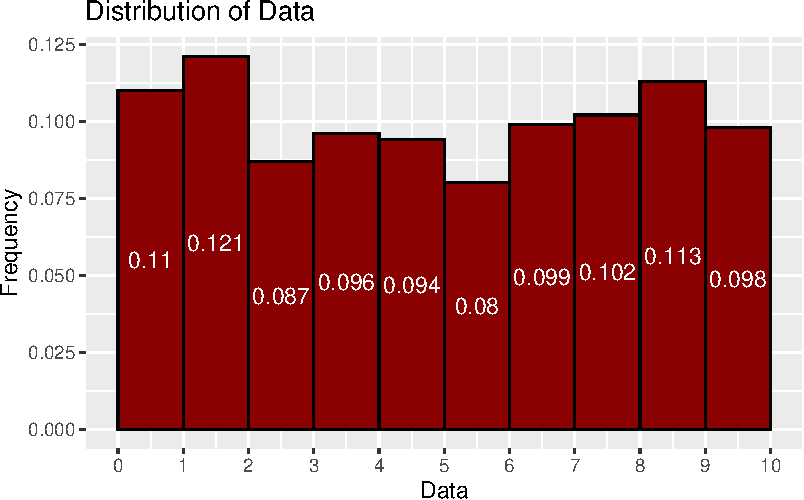
\includegraphics{Qualitative_and_Quantitative_Variables_files/figure-pdf/unnamed-chunk-4-1.pdf}

For continuous variables, it doesn't make since to have a histogram for
each individual values like we did for discrete variables. If we tried
this then we might need an \textbf{infinte} amount of bars or more!
Instead, we group the data into intervals (bins) of the same length and
then create a histogram based on these intervals. This is what we did
above. We grouped the data into intervals of 1 and then created a
histogram based on the intervals (0,1), (1, 2), (2, 3), etc. For this
histogram the bars represent the proportions (rounded to 3 decimal
places) of the data that fall into each interval. If you look at the
second bar in the histogram, you will see the number \texttt{0.121} in
the bar. This means that 12.1\% of the data falls into the interval (1,
2).

\bookmarksetup{startatroot}

\chapter*{Categorial Variables.}\label{categorial-variables.}
\addcontentsline{toc}{chapter}{Categorial Variables.}

\markboth{Categorial Variables.}{Categorial Variables.}

Descriptive statistics are the first pieces of information used to
understand and represent a dataset. Their goal, in essence, is to
describe the main features of numerical and categorical information with
simple summaries. These summaries can be presented with a single numeric
measure, using summary tables, or via graphical representation. Here, I
illustrate the most common forms of descriptive statistics for
categorical data but keep in mind there are numerous ways to describe
and illustrate key features of data.

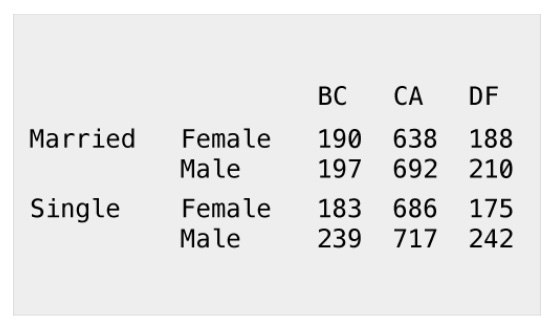
\includegraphics[width=0.35\textwidth,height=\textheight]{./images/Daily-6-Pic-1.jpg}

This tutorial covers the key features we are initially interested in
understanding for categorical data, to include:

\begin{itemize}
\tightlist
\item
  Frequencies: The number of observations for a particular category
\item
  Proportions: The percent that each category accounts for out of the
  whole
\item
  Marginals: The totals in a cross tabulation by row or column
\end{itemize}

\textbf{Replication Requirements}

To illustrate ways to compute these summary statistics and to visualize
categorical data, I'll demonstrate using this data which contains
artificial supermarket transaction data and can be found on our Canvas
page :

\textbf{Supermarket Transaction.xls}

Posit Cloud is running on a server, not your computer. To access a file
on your local drive, you need to upload it to the server. Click on the
Files tab (in the lower right pane) then on Upload. In the Upload Files
dialog, click on Choose File, navigate to the file and click on Open.
You can also change the target directory for the upload.

In addition, the packages we will need include the following:

\begin{Shaded}
\begin{Highlighting}[]
\CommentTok{\# install.packages("tidyverse")}
\FunctionTok{library}\NormalTok{(readxl)                   }\CommentTok{\# for reading in excel spreadsheet}
\end{Highlighting}
\end{Shaded}

First, let's read in the data. The data frame consists of 16 variables,
which I illustrate a select few below:

\begin{Shaded}
\begin{Highlighting}[]
\NormalTok{supermarket }\OtherTok{\textless{}{-}} \FunctionTok{read\_excel}\NormalTok{(}\StringTok{"./Supermarket Transactions.xlsx"}\NormalTok{)}

\CommentTok{\# Check out the first few lines but only columns 3,4,5,8,9,14,15,16}

\CommentTok{\# These are the 8 variables : Customer ID, Gender, Marital Status, Annual Income,}
\CommentTok{\# City, Product Category, Units Sold, Revenue}

\FunctionTok{head}\NormalTok{(supermarket[, }\FunctionTok{c}\NormalTok{(}\DecValTok{3}\SpecialCharTok{:}\DecValTok{5}\NormalTok{,}\DecValTok{8}\SpecialCharTok{:}\DecValTok{9}\NormalTok{,}\DecValTok{14}\SpecialCharTok{:}\DecValTok{16}\NormalTok{)])}
\end{Highlighting}
\end{Shaded}

\begin{verbatim}
# A tibble: 6 x 8
  `Customer ID` Gender `Marital Status` `Annual Income` City  `Product Category`
          <dbl> <chr>  <chr>            <chr>           <chr> <chr>             
1          7223 F      S                $30K - $50K     Los ~ Snack Foods       
2          7841 M      M                $70K - $90K     Los ~ Vegetables        
3          8374 F      M                $50K - $70K     Brem~ Snack Foods       
4          9619 M      M                $30K - $50K     Port~ Candy             
5          1900 F      S                $130K - $150K   Beve~ Carbonated Bevera~
6          6696 F      M                $10K - $30K     Beve~ Side Dishes       
# i 2 more variables: `Units Sold` <dbl>, Revenue <dbl>
\end{verbatim}

\textbf{Frequencies}

To produce \textbf{contingency tables} which calculate counts for each
combination of categorical variables we can use R's \textbf{table( )}
function. For instance, we may want to get the total count of female and
male customers.

\begin{Shaded}
\begin{Highlighting}[]
\FunctionTok{table}\NormalTok{(supermarket}\SpecialCharTok{$}\NormalTok{Gender)}
\end{Highlighting}
\end{Shaded}

\begin{verbatim}

   F    M 
7170 6889 
\end{verbatim}

If we want to understand the number of married and single females and
male customers we can produce a cross classification table:

\begin{Shaded}
\begin{Highlighting}[]
\CommentTok{\# cross classication counts for gender by marital status}

\FunctionTok{table}\NormalTok{(supermarket}\SpecialCharTok{$}\StringTok{\textasciigrave{}}\AttributeTok{Marital Status}\StringTok{\textasciigrave{}}\NormalTok{, supermarket}\SpecialCharTok{$}\NormalTok{Gender)}
\end{Highlighting}
\end{Shaded}

\begin{verbatim}
   
       F    M
  M 3602 3264
  S 3568 3625
\end{verbatim}

We can also produce multidimensional tables based on three or more
categorical variables. For this, we leverage the \textbf{ftable( )}
function to print the results more attractively. In this case we assess
the count of customers by marital status, gender, and location:

\begin{Shaded}
\begin{Highlighting}[]
\CommentTok{\# customer counts across location by gender and marital status}

\NormalTok{table1 }\OtherTok{\textless{}{-}} \FunctionTok{table}\NormalTok{(supermarket}\SpecialCharTok{$}\StringTok{\textasciigrave{}}\AttributeTok{Marital Status}\StringTok{\textasciigrave{}}\NormalTok{, supermarket}\SpecialCharTok{$}\NormalTok{Gender, supermarket}\SpecialCharTok{$}\StringTok{\textasciigrave{}}\AttributeTok{State or Province}\StringTok{\textasciigrave{}}\NormalTok{)}

\CommentTok{\# Remember that the previous command is taking the table we are creating and saving it into}
\CommentTok{\# a new variable called "table1". We will now take this table and evaluate it }
\CommentTok{\# using the **ftable( )** command.}

\FunctionTok{ftable}\NormalTok{(table1)}
\end{Highlighting}
\end{Shaded}

\begin{verbatim}
       BC   CA   DF Guerrero Jalisco   OR Veracruz   WA Yucatan Zacatecas
                                                                         
M F   190  638  188       77      15  510      142 1166     200       476
  M   197  692  210       94       5  514      108 1160     129       155
S F   183  686  175      107      30  607      125 1134     164       357
  M   239  717  242      105      25  631       89 1107     161       309
\end{verbatim}

\textbf{Proportions}

We can also produce contingency tables that present the proportions
(percentages) of each category or combination of categories. To do this
we simply feed the frequency tables produced by \textbf{table( )} to the
\textbf{prop.table( )} function. The following reproduces the previous
tables but calculates the proportions rather than counts:

\begin{Shaded}
\begin{Highlighting}[]
\CommentTok{\# Calculate the percentages of gender categories}

\CommentTok{\# We will first create a new table so we don\textquotesingle{}t accidentally hurt our previous work.}

\NormalTok{table2 }\OtherTok{\textless{}{-}} \FunctionTok{table}\NormalTok{(supermarket}\SpecialCharTok{$}\NormalTok{Gender)}

\CommentTok{\# After saving the output ( new table) to the variable table2, we will now send}
\CommentTok{\# this table2 to prop.table( ).}

\FunctionTok{prop.table}\NormalTok{(table2)}
\end{Highlighting}
\end{Shaded}

\begin{verbatim}

        F         M 
0.5099936 0.4900064 
\end{verbatim}

Based on the output, we can see that there are about 51\% of respondents
saying they are female (F) and about 49\% of the respondents saying they
are male (M).

We could also create a two-way table by adding another variable. For
example, let's create a table that tallies up the variables
\textbf{Marital Status} and \textbf{Gender}.

\begin{Shaded}
\begin{Highlighting}[]
\CommentTok{\# We shall create a new table (table3) to analyze. }

\NormalTok{table3 }\OtherTok{\textless{}{-}} \FunctionTok{table}\NormalTok{(supermarket}\SpecialCharTok{$}\StringTok{\textasciigrave{}}\AttributeTok{Marital Status}\StringTok{\textasciigrave{}}\NormalTok{, supermarket}\SpecialCharTok{$}\NormalTok{Gender)}

\CommentTok{\# We can now create a table of proportions for these variables.}

\FunctionTok{prop.table}\NormalTok{(table3)}
\end{Highlighting}
\end{Shaded}

\begin{verbatim}
   
            F         M
  M 0.2562060 0.2321644
  S 0.2537876 0.2578420
\end{verbatim}

We can interpret this tables as follows :

\begin{itemize}
\tightlist
\item
  25.6\% of the respondents identify as Female (F) and Married (M)
\item
  23.2\% of the respondents identify as Male (M) and Married (M)
\item
  25.3\% of the respondents identify as Female (F) and Single (S)
\item
  25.8\% of the respondents identify as Male (M) and Single (S)
\end{itemize}

Note that we can tell \textbf{ftable( )} how many decimal place to use
when reporting the results. For example, go back to table 1. We can
combine several commands together into one :

\begin{itemize}
\tightlist
\item
  We want to run \textbf{prop.table( )} on table 1
\item
  We want to limit to 3 decimal places
\item
  We want to round the results
\item
  We want to take this result and use \textbf{ftable( )}
\end{itemize}

\begin{Shaded}
\begin{Highlighting}[]
\FunctionTok{ftable}\NormalTok{(}\FunctionTok{round}\NormalTok{(}\FunctionTok{prop.table}\NormalTok{(table1), }\DecValTok{3}\NormalTok{))}
\end{Highlighting}
\end{Shaded}

\begin{verbatim}
        BC    CA    DF Guerrero Jalisco    OR Veracruz    WA Yucatan Zacatecas
                                                                              
M F  0.014 0.045 0.013    0.005   0.001 0.036    0.010 0.083   0.014     0.034
  M  0.014 0.049 0.015    0.007   0.000 0.037    0.008 0.083   0.009     0.011
S F  0.013 0.049 0.012    0.008   0.002 0.043    0.009 0.081   0.012     0.025
  M  0.017 0.051 0.017    0.007   0.002 0.045    0.006 0.079   0.011     0.022
\end{verbatim}

\textbf{Marginals}

Marginals show the total counts or percentages across columns or rows in
a contingency table. For instance, if we go back to table3 which is the
cross classification counts for gender by marital status:

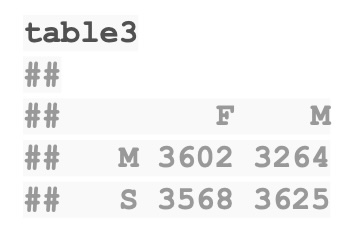
\includegraphics[width=0.2\textwidth,height=\textheight]{./images/Daily-6-Pic-2.jpg}

The \textbf{margins} are simply the sums of the rows and the columns.
For example, if we look at table3, I might want to know, ``How many
respondents identify as Single?'' This is the sum on the last row, 3568
+ 3625 = 7,193. Similarly, the amount of those identifying as Married
would be 3602 + 3264 = 6,866. We can calculate these values using the
\textbf{margin.table( )} command.

\begin{Shaded}
\begin{Highlighting}[]
\CommentTok{\# FREQUENCY MARGINALS}
\CommentTok{\# row marginals {-} totals for each marital status across gender}

\FunctionTok{margin.table}\NormalTok{(table3, }\DecValTok{1}\NormalTok{)}
\end{Highlighting}
\end{Shaded}

\begin{verbatim}

   M    S 
6866 7193 
\end{verbatim}

\begin{Shaded}
\begin{Highlighting}[]
\CommentTok{\# This command takes in the table for which we want to find the margins.}
\CommentTok{\# The second parameter tells us if we want row (1) or column (2) margins.}
\end{Highlighting}
\end{Shaded}

We can see that this example verifes the values we calculated above.

We could also calculate the column margins by changing the second
parameter to 2. It is left to you to verify that these values are
correct.

\begin{Shaded}
\begin{Highlighting}[]
\CommentTok{\# column marginals {-} totals for each gender across marital status}

\FunctionTok{margin.table}\NormalTok{(table3, }\DecValTok{2}\NormalTok{)}
\end{Highlighting}
\end{Shaded}

\begin{verbatim}

   F    M 
7170 6889 
\end{verbatim}

If we were more interested in proportions / percentage rather than
counts, we could use the \textbf{prop.table( )} command to calculate
these proportions. The first example will calculate the row percentages.

\begin{Shaded}
\begin{Highlighting}[]
\CommentTok{\# PERCENTAGE MARGINALS}

\CommentTok{\# row marginals {-} row percentages across gender}

\FunctionTok{prop.table}\NormalTok{(table3, }\AttributeTok{margin =} \DecValTok{1}\NormalTok{)}
\end{Highlighting}
\end{Shaded}

\begin{verbatim}
   
            F         M
  M 0.5246140 0.4753860
  S 0.4960378 0.5039622
\end{verbatim}

We could easily calcuate the column percentages using the following
command.

\begin{Shaded}
\begin{Highlighting}[]
\CommentTok{\# column marginals {-} column percentages across marital status}

\FunctionTok{prop.table}\NormalTok{(table3, }\AttributeTok{margin =} \DecValTok{2}\NormalTok{)}
\end{Highlighting}
\end{Shaded}

\begin{verbatim}
   
            F         M
  M 0.5023710 0.4737988
  S 0.4976290 0.5262012
\end{verbatim}

\bookmarksetup{startatroot}

\chapter*{Intro to R}\label{intro-to-r}
\addcontentsline{toc}{chapter}{Intro to R}

\markboth{Intro to R}{Intro to R}

In this section we are going to go through some of the basics to
programming in R. We will look at how to comment your work, basic
calculator computations, create a variable, create a vector, how to
install a library / package, and use some of the built-in functions.

\section*{Comments}\label{comments}
\addcontentsline{toc}{section}{Comments}

\markright{Comments}

Comments are a very important part of coding. When you are writing code,
you will want to leave notes to yourself and your collaborators to
describe what you are doing at each step. You can also leave notes on
parts of the code that are norking or that you feel should be changed.
It is a way to remind yourself and your collaborators the work that has
been done, why it was done, what is broken, other changes you want to
make, and more. They are especially important when you come back to the
code after not having looked at it for a while.

Basically, leave as many comments as possible while coding. You should
start with the names of those that are working on the project with a
synopsis on what is the purpose of the project.

A comment is any text following a hashtag (\#) on the same line. This
text is ignored by the R compiler and does not affect how the script is
run. This is an example of how you should start every script you write
in this class or at your job.

\begin{Shaded}
\begin{Highlighting}[]
\CommentTok{\# Mike LeVan}
\CommentTok{\# Data{-}1004 Data Analytics and Statistics}
\CommentTok{\# Date}

\CommentTok{\# Assignment Description}

\CommentTok{\# I can write out notes to myself and my colleagues!}

\CommentTok{\# R ignores all the lines that start with \#}
\end{Highlighting}
\end{Shaded}

\section*{Calculator}\label{calculator}
\addcontentsline{toc}{section}{Calculator}

\markright{Calculator}

While this is quite a bit of overkill, R can be used as a basic
calculator. Here are the operators :

\subsection*{Addition ( + )}\label{addition}
\addcontentsline{toc}{subsection}{Addition ( + )}

\begin{Shaded}
\begin{Highlighting}[]
\CommentTok{\# This is an example of addition.}

\DecValTok{4} \SpecialCharTok{+} \DecValTok{8}
\end{Highlighting}
\end{Shaded}

\begin{verbatim}
[1] 12
\end{verbatim}

Notice the output above :

\texttt{{[}1{]}\ 12}

The {[}1{]} means the first output followed the by value of the output
12.

\subsection*{Subtraction ( - )}\label{subtraction--}
\addcontentsline{toc}{subsection}{Subtraction ( - )}

\begin{Shaded}
\begin{Highlighting}[]
\CommentTok{\# Here is an example of subtraction.}

\DecValTok{5} \SpecialCharTok{{-}} \DecValTok{14}
\end{Highlighting}
\end{Shaded}

\begin{verbatim}
[1] -9
\end{verbatim}

\subsection*{Multiplication ( * )}\label{multiplication}
\addcontentsline{toc}{subsection}{Multiplication ( * )}

\begin{Shaded}
\begin{Highlighting}[]
\CommentTok{\# Here is an example of multiplication}

\DecValTok{8} \SpecialCharTok{*} \DecValTok{17}
\end{Highlighting}
\end{Shaded}

\begin{verbatim}
[1] 136
\end{verbatim}

\subsection*{Division ( / )}\label{division}
\addcontentsline{toc}{subsection}{Division ( / )}

\begin{Shaded}
\begin{Highlighting}[]
\CommentTok{\# Division}

\DecValTok{22} \SpecialCharTok{/} \DecValTok{7}
\end{Highlighting}
\end{Shaded}

\begin{verbatim}
[1] 3.142857
\end{verbatim}

\subsection*{Exponentiation ( \^{} )}\label{exponentiation}
\addcontentsline{toc}{subsection}{Exponentiation ( \^{} )}

\begin{Shaded}
\begin{Highlighting}[]
\CommentTok{\# Exponentiation}

\DecValTok{5}\SpecialCharTok{\^{}}\DecValTok{3}
\end{Highlighting}
\end{Shaded}

\begin{verbatim}
[1] 125
\end{verbatim}

\subsection*{Square Roots and Radicals}\label{square-roots-and-radicals}
\addcontentsline{toc}{subsection}{Square Roots and Radicals}

Recall that we can use exponents to calculate radicals, too. If you
recall, the square root function is the same as raising a value to the
(1 / 2) power!

\begin{Shaded}
\begin{Highlighting}[]
\CommentTok{\# Here is the square root of 9}

\DecValTok{9}\SpecialCharTok{\^{}}\NormalTok{(}\DecValTok{1}\SpecialCharTok{/}\DecValTok{2}\NormalTok{)}
\end{Highlighting}
\end{Shaded}

\begin{verbatim}
[1] 3
\end{verbatim}

Notice that there are some levels of estimation / rounding here. For
example, calculate the square root of 2

\begin{Shaded}
\begin{Highlighting}[]
\DecValTok{2}\SpecialCharTok{\^{}}\NormalTok{(}\DecValTok{1}\SpecialCharTok{/}\DecValTok{2}\NormalTok{)}
\end{Highlighting}
\end{Shaded}

\begin{verbatim}
[1] 1.414214
\end{verbatim}

Obviously the real answer goes further than six decimal places. Also
think about the square root of 2 multiplied by itself. We should get the
value 2 right back :

\begin{Shaded}
\begin{Highlighting}[]
\DecValTok{2}\SpecialCharTok{\^{}}\NormalTok{(}\DecValTok{1}\SpecialCharTok{/}\DecValTok{2}\NormalTok{) }\SpecialCharTok{*} \DecValTok{2}\SpecialCharTok{\^{}}\NormalTok{(}\DecValTok{1}\SpecialCharTok{/}\DecValTok{2}\NormalTok{)}
\end{Highlighting}
\end{Shaded}

\begin{verbatim}
[1] 2
\end{verbatim}

But notice what happens if we then subtract 2 from the previous result :

\begin{Shaded}
\begin{Highlighting}[]
\DecValTok{2}\SpecialCharTok{\^{}}\NormalTok{(}\DecValTok{1}\SpecialCharTok{/}\DecValTok{2}\NormalTok{) }\SpecialCharTok{*} \DecValTok{2}\SpecialCharTok{\^{}}\NormalTok{(}\DecValTok{1}\SpecialCharTok{/}\DecValTok{2}\NormalTok{) }\SpecialCharTok{{-}} \DecValTok{2}
\end{Highlighting}
\end{Shaded}

\begin{verbatim}
[1] 4.440892e-16
\end{verbatim}

This result is in scientific notation, but what does it mean? When you
see the ``e-16'' part, that says to move the decimal places 16 spots to
the left, so this answer is closer to 0.000000000000000440892. Notice
that it is not zero, as it should be. This is because of the estimation
that was talked about above.

\subsection*{Creating a variable}\label{creating-a-variable}
\addcontentsline{toc}{subsection}{Creating a variable}

What is a variable? Imagine dumping some data in a bucket and then
giving that bucket a name. Now, every time you use that name, you are
really referring to what is in the bucket.

NOTE 1 : Recall our discussion from class about naming your variables.
You want to pick a name for your variables that make sense. It will make
editing your script much easier in the long run. If I called a variable
``Quiz\_Scores'' then we know what types of values we are working with.
If I called the variable ``x'' instead, what does that tell us about the
variable itself?

We can use an ``arrow'' to assign a value into a variable. An arrow is
just a less than sign followed by a dash with no spaces between them :

\texttt{\textless{}-}

For example, what if I wanted to assign the value 3 into a variable
called ``x'' and the value 7 into a variable called ``y'', we could type
this into our R script :

\begin{Shaded}
\begin{Highlighting}[]
\CommentTok{\# Assign 3 to the variable "x"}

\NormalTok{x }\OtherTok{\textless{}{-}} \DecValTok{3}

\CommentTok{\# Assign 7 to the variable "y"}

\NormalTok{y }\OtherTok{\textless{}{-}} \DecValTok{7}
\end{Highlighting}
\end{Shaded}

NOTE 2 : At this point you should look at the ENVIRONMENT window. This
window shows you the variables you are using and the values they
contain.

Now that we have values in these variables, we can now use them in our
script. For example, what if I wanted to perform some basic calculations
with these variables :

\subsection*{Addition of two variables : x +
y}\label{addition-of-two-variables-x-y}
\addcontentsline{toc}{subsection}{Addition of two variables : x + y}

\begin{Shaded}
\begin{Highlighting}[]
\CommentTok{\# We are going to calculate x + y. }

\CommentTok{\# Recall that x = 3 and y = 7 from above, so this should return 10}

\NormalTok{x }\SpecialCharTok{+}\NormalTok{ y}
\end{Highlighting}
\end{Shaded}

\begin{verbatim}
[1] 10
\end{verbatim}

We could do the same for several different operations :

\begin{Shaded}
\begin{Highlighting}[]
\CommentTok{\# Example 1 : Subtract two variables :}

\NormalTok{y }\SpecialCharTok{{-}}\NormalTok{ x}
\end{Highlighting}
\end{Shaded}

\begin{verbatim}
[1] 4
\end{verbatim}

\begin{Shaded}
\begin{Highlighting}[]
\CommentTok{\# Example 2 : Multiply a variable by a constant. We could multiply the variable x by 9 to}
\CommentTok{\# get 9 * 3 = 27}

\DecValTok{9}\SpecialCharTok{*}\NormalTok{x}
\end{Highlighting}
\end{Shaded}

\begin{verbatim}
[1] 27
\end{verbatim}

\begin{Shaded}
\begin{Highlighting}[]
\CommentTok{\# Example 3 : Take a linear combination of two different variables. For example, we can}
\CommentTok{\# multiply your by 2 and x by 3 and add them together to get }
\CommentTok{\# 2*7 + 3*3 = 13 + 9 = 23 }

\DecValTok{2}\SpecialCharTok{*}\NormalTok{y }\SpecialCharTok{+} \DecValTok{3}\SpecialCharTok{*}\NormalTok{x}
\end{Highlighting}
\end{Shaded}

\begin{verbatim}
[1] 23
\end{verbatim}

\begin{Shaded}
\begin{Highlighting}[]
\CommentTok{\# Example 4 : Use one variable as an exponent for another variable. In this case, take the }
\CommentTok{\# variable x and raise it to the power y. In this case, we are computing 3 \^{} 7}
\CommentTok{\# which is 3 * 3 * 3 * 3 * 3 * 3 * 3 = 2187:}

\NormalTok{x}\SpecialCharTok{\^{}}\NormalTok{y}
\end{Highlighting}
\end{Shaded}

\begin{verbatim}
[1] 2187
\end{verbatim}

\subsection*{Assigning Operations to
Variables}\label{assigning-operations-to-variables}
\addcontentsline{toc}{subsection}{Assigning Operations to Variables}

We could also take the result from an operation and assign that to a
different variable. For exampe, we could multiply x by 7 and multiply y
by 2, subtract them and store the result in a new variable z.

\begin{Shaded}
\begin{Highlighting}[]
\NormalTok{z }\OtherTok{\textless{}{-}} \DecValTok{7}\SpecialCharTok{*}\NormalTok{x }\SpecialCharTok{{-}} \DecValTok{2}\SpecialCharTok{*}\NormalTok{y}
\end{Highlighting}
\end{Shaded}

If you want to print out what is now in the variable z, you can now see
it in the ENVIRONMENT window. You can also type it out in the script :

\begin{Shaded}
\begin{Highlighting}[]
\CommentTok{\# Print out the variable z}

\NormalTok{z}
\end{Highlighting}
\end{Shaded}

\begin{verbatim}
[1] 7
\end{verbatim}

Recall from class that there are different kinds of variables we might
be asked to consider. We could have QUANTITATIVE data that could be in
the form of continuous or discrete values. Another kind of data we
talked about was CATEGORICAL data. Depending on the type of data you are
analyzing, you would need to perform different operations.

\subsection*{Creating vectors}\label{creating-vectors}
\addcontentsline{toc}{subsection}{Creating vectors}

Let's assume the class takes a quiz and I want to keep track of them.
Instead of creating a variable for each individual quiz, I can create
one vector that will have all of the scores.

For example, if I have the quiz scores 10, 5, 8, 9, 4 then I could
create the variables Student\_1\_Quiz, Student\_2\_Quiz, etc. It is much
easier to create a single variable that holds all of these values.

We will use the following command : \textbf{c( )}

The ``\textbf{c}'' is shorthand for ``\textbf{concatenate}'' which means
to link objects together in a chain or series.

If I wanted to create a vector for the quiz scores above, I would create
a vector called Quiz1\_Scores and assign the variables as follows :

Notice the order is important. If we want to assign the first student a
10, the second a 5, the third an 8, the fourth a 9, and the fifth a 4,
then we would do the following :

\begin{Shaded}
\begin{Highlighting}[]
\CommentTok{\# Create a vector and call it "Quiz1\_Scores" }

\NormalTok{Quiz1\_Scores }\OtherTok{\textless{}{-}} \FunctionTok{c}\NormalTok{(}\DecValTok{10}\NormalTok{, }\DecValTok{5}\NormalTok{, }\DecValTok{8}\NormalTok{, }\DecValTok{9}\NormalTok{ ,}\DecValTok{4}\NormalTok{)}
\end{Highlighting}
\end{Shaded}

Notice how this is represented in the ENVIRONMENT window :

\begin{Shaded}
\begin{Highlighting}[]
\CommentTok{\# We can print out the variable to check what it contains}

\NormalTok{Quiz1\_Scores     }
\end{Highlighting}
\end{Shaded}

\begin{verbatim}
[1] 10  5  8  9  4
\end{verbatim}

This tells us the scores are located in spots 1, 2, 3, 4, 5 in the
vector. In this vector, the values in the spots are then shown as the
values : 10 5 8 9 4

Let's say Student 3 comes to see us and ask about their quiz grade. We
can then access the individual value as follows :

\begin{Shaded}
\begin{Highlighting}[]
\NormalTok{Quiz1\_Scores[}\DecValTok{3}\NormalTok{]}
\end{Highlighting}
\end{Shaded}

\begin{verbatim}
[1] 8
\end{verbatim}

If we wanted the fifth value in the vector we could say :

\begin{Shaded}
\begin{Highlighting}[]
\NormalTok{Quiz1\_Scores[}\DecValTok{5}\NormalTok{]}
\end{Highlighting}
\end{Shaded}

\begin{verbatim}
[1] 4
\end{verbatim}

If we wanted to print out the 3rd, 4th, and 5th scores, we could say :

\begin{Shaded}
\begin{Highlighting}[]
\NormalTok{Quiz1\_Scores[}\DecValTok{3}\SpecialCharTok{:}\DecValTok{5}\NormalTok{]}
\end{Highlighting}
\end{Shaded}

\begin{verbatim}
[1] 8 9 4
\end{verbatim}

Obviously we would want to make sure we enter in the data in an
appropriate order because if I rearrange the order I get a completely
different vector :

\begin{Shaded}
\begin{Highlighting}[]
\NormalTok{Quiz1\_Scores\_B }\OtherTok{\textless{}{-}} \FunctionTok{c}\NormalTok{(}\DecValTok{5}\NormalTok{, }\DecValTok{10}\NormalTok{, }\DecValTok{4}\NormalTok{, }\DecValTok{9}\NormalTok{, }\DecValTok{8}\NormalTok{)}
\end{Highlighting}
\end{Shaded}

While I have the same scores, they are located in different spots of the
vectors and would assign different values to Student 1, Student 2, etc.

We could also use characters in our vectors. We would need to make sure
we use quotation marks so the compiler does not think we are using other
variables in our vector.

\begin{Shaded}
\begin{Highlighting}[]
\NormalTok{Students }\OtherTok{\textless{}{-}} \FunctionTok{c}\NormalTok{(}\StringTok{"Alice"}\NormalTok{, }\StringTok{"Bob"}\NormalTok{, }\StringTok{"Chad"}\NormalTok{, }\StringTok{"Debbie"}\NormalTok{, }\StringTok{"Eric"}\NormalTok{)}
\end{Highlighting}
\end{Shaded}

Check out what is now in the ENVIRONMENT window :

\begin{Shaded}
\begin{Highlighting}[]
\CommentTok{\# Print out the Students vector :}

\NormalTok{Students}
\end{Highlighting}
\end{Shaded}

\begin{verbatim}
[1] "Alice"  "Bob"    "Chad"   "Debbie" "Eric"  
\end{verbatim}

The only real difference from above is the we are using characters
instead of numeric values and that is identified because of the ``chr''
notation in the description.

We can look at the individual entries jsut as we did above. To look at
the fourth entry in the vector we would type :

\begin{Shaded}
\begin{Highlighting}[]
\NormalTok{Students[}\DecValTok{4}\NormalTok{]}
\end{Highlighting}
\end{Shaded}

\begin{verbatim}
[1] "Debbie"
\end{verbatim}

If you are given a variable or vector and want to know what type of
values it contains, you can use the ``class'' command to tell you. Here
are some examples to check entire vectors or individual locations in a
vector :

\begin{Shaded}
\begin{Highlighting}[]
\FunctionTok{class}\NormalTok{(Quiz1\_Scores)}
\end{Highlighting}
\end{Shaded}

\begin{verbatim}
[1] "numeric"
\end{verbatim}

\begin{Shaded}
\begin{Highlighting}[]
\FunctionTok{class}\NormalTok{(Quiz1\_Scores[}\DecValTok{2}\NormalTok{])}
\end{Highlighting}
\end{Shaded}

\begin{verbatim}
[1] "numeric"
\end{verbatim}

\begin{Shaded}
\begin{Highlighting}[]
\FunctionTok{class}\NormalTok{(Students)}
\end{Highlighting}
\end{Shaded}

\begin{verbatim}
[1] "character"
\end{verbatim}

\begin{Shaded}
\begin{Highlighting}[]
\FunctionTok{class}\NormalTok{(Students[}\DecValTok{1}\NormalTok{])}
\end{Highlighting}
\end{Shaded}

\begin{verbatim}
[1] "character"
\end{verbatim}

\begin{Shaded}
\begin{Highlighting}[]
\FunctionTok{class}\NormalTok{(Students)}
\end{Highlighting}
\end{Shaded}

\begin{verbatim}
[1] "character"
\end{verbatim}

What happens if we mix our variables and have numbers and characters in
the same vector?

Here is how one could be created :

\begin{Shaded}
\begin{Highlighting}[]
\NormalTok{blah }\OtherTok{\textless{}{-}} \FunctionTok{c}\NormalTok{(}\DecValTok{4}\NormalTok{, }\StringTok{"dffdg"}\NormalTok{, }\DecValTok{6}\NormalTok{, }\DecValTok{9}\NormalTok{, }\StringTok{"trte"}\NormalTok{)}
\end{Highlighting}
\end{Shaded}

How does R interpret these values?

\begin{Shaded}
\begin{Highlighting}[]
\FunctionTok{class}\NormalTok{(blah)}
\end{Highlighting}
\end{Shaded}

\begin{verbatim}
[1] "character"
\end{verbatim}

Notice that it considers EVERY entry in this vector to be a CHARACTER
even though we entered some as numbers. Be careful with this as it could
cause issues on how we work and interact with this vector.

\subsection*{Libraries and Packages}\label{libraries-and-packages}
\addcontentsline{toc}{subsection}{Libraries and Packages}

When we start up a session of R, there are some commands that are
already built into the program that we can use. For instance, we used
the basic mathematics operations above.

You will eventually want to do a deeper analysis of the data that needs
a command that is not already installed in your current session of R.
This is where the idea of Libraries or Packages comes into play.

If there is a command we want to use that is not currently loaded into
R, we can install the package that includes the command.

You can see what is loaded already by clicking on the PACKAGES tab.

You will see the packages that are loaded up as they will have a check
mark indicated they have been installed.

Let's say there was something in the ``\textbf{tcltk}'' library I wanted
to use. I could then click on the check box for ``\textbf{tcltk}'' and a
message should come up in the Console showing that the package was
installed.

\textbf{\textgreater{} library(tcltk, lib.loc =
``/opt/R/4.3.1/lib/R/library'')}

We could remove the package by unclicking on the check box. We get a
confirmation in the Console :

\textbf{\textgreater{} detach(``package:tcltk'', unload = TRUE)}

What happens if we need a package that is not included in the list.
There are hundreds of packages that people have developed to use in R.

For example, consider the \textbf{tidyverse} library. This is a library
that contains several commands that we will be using over the semester.

If we know we are going to be using a specific library in our R script,
then we should install it at the top of the script. We would enter in a
command such as : \textbf{install.packages(``tidyverse'')}

Once we do this, you will see several different commands that are now
available for us to use to analyze our data set.

If you look at the Packages tab, you will see several new packages that
we can add to use in the program.

\textbf{tidyverse} comes with several packages. If you click on the
tidyverse package, you will see several packages installed :

\textbf{\textgreater{} library(tidyverse)}

── Attaching core tidyverse packages ────────────────────── tidyverse
2.0.0 ──

✔ dplyr 1.1.2 ✔ readr 2.1.4

✔ forcats 1.0.0 ✔ stringr 1.5.0

✔ ggplot2 3.4.2 ✔ tibble 3.2.1

✔ lubridate 1.9.2 ✔ tidyr 1.3.0

✔ purrr 1.0.1\\

These packages are now loaded into R. Note that is we uncheck the
tidyverse package, these are still loaded into R. We can remove them by
unchecking their package. For example, if I uncheck the ggplot2 package
you will see the following message :

\texttt{\textgreater{}\ detach("package:ggplot2",\ unload\ =\ TRUE)}

When you are starting to become a programmer it might be tempting just
to load up EVERYTING, but that is not good practice. When these packages
are loaded up, they are taking up memory. This can lead to slower
computation times as well as lead to larger files being generated,
wasting space. Try to be efficient and load up what you need and avoid
bloat.

\subsection*{Functions}\label{functions}
\addcontentsline{toc}{subsection}{Functions}

There are two kinds of functions we are going to deal with in class -
the ones that are built into R and ones we create ourselves. This lesson
will only consider the functions that are built in.

A \textbf{FUNCTION} is a command that takes in some kind of data,
manipulates it, and returns a value. It has the following form :

\textbf{FUNCTION\_NAME( data )}

This will simply print out the result. Remember we could also assign the
result to a variable.

\textbf{result \textless- FUNCTION\_NAME ( data)}

For example, go back to the quiz grades we had listed earlier. What if I
wanted to calculated the average (mean) of the quiz scores? I could
enter the following :

\begin{Shaded}
\begin{Highlighting}[]
\FunctionTok{mean}\NormalTok{(Quiz1\_Scores)}
\end{Highlighting}
\end{Shaded}

\begin{verbatim}
[1] 7.2
\end{verbatim}

I could assign the result to a variable, such as :

\begin{Shaded}
\begin{Highlighting}[]
\CommentTok{\# Calculate the average and store the result in the variable }
\CommentTok{\# named "Quiz1\_Average"}

\NormalTok{Quiz1\_Average }\OtherTok{\textless{}{-}} \FunctionTok{mean}\NormalTok{(Quiz1\_Scores)}

\CommentTok{\# Print out the average}

\NormalTok{Quiz1\_Average}
\end{Highlighting}
\end{Shaded}

\begin{verbatim}
[1] 7.2
\end{verbatim}

There are several other built in functions. Here are a few :

\textbf{min( ), max( ), mean( ), median( ), sum( ), range( ), abs( )}

If we wanted the highest quiz grade, we could say :

\begin{Shaded}
\begin{Highlighting}[]
\CommentTok{\# Find the maximum value :}

\FunctionTok{max}\NormalTok{(Quiz1\_Scores)}
\end{Highlighting}
\end{Shaded}

\begin{verbatim}
[1] 10
\end{verbatim}

If I wanted to know how many values are in my vector, I could say :

\begin{Shaded}
\begin{Highlighting}[]
\CommentTok{\# Use the length function :}

\FunctionTok{length}\NormalTok{(Quiz1\_Scores)}
\end{Highlighting}
\end{Shaded}

\begin{verbatim}
[1] 5
\end{verbatim}

If I wanted to pick a random number from 1 - 100, I could type the
following

\begin{Shaded}
\begin{Highlighting}[]
\FunctionTok{sample}\NormalTok{(}\DecValTok{100}\NormalTok{,}\DecValTok{1}\NormalTok{)}
\end{Highlighting}
\end{Shaded}

\begin{verbatim}
[1] 21
\end{verbatim}

If I wanted to pick three random numbers (all different) from 1 - 100,
we could say this :

\begin{Shaded}
\begin{Highlighting}[]
\FunctionTok{sample}\NormalTok{(}\DecValTok{100}\NormalTok{,}\DecValTok{3}\NormalTok{)}
\end{Highlighting}
\end{Shaded}

\begin{verbatim}
[1] 61 75 20
\end{verbatim}

If I wanted to pick seven random numbers from 1 - 100 where we could
have (but not guarantee) duplicate values, I could say this :

\begin{Shaded}
\begin{Highlighting}[]
\FunctionTok{sample}\NormalTok{(}\DecValTok{100}\NormalTok{, }\DecValTok{7}\NormalTok{, }\AttributeTok{replace=}\ConstantTok{TRUE}\NormalTok{)}
\end{Highlighting}
\end{Shaded}

\begin{verbatim}
[1]  81  67  13  70   3 100  20
\end{verbatim}

To create a random vector for a range of values, we can use sample
function. We just need to pass the range and the sample size inside the
sample function.

For example, if we want to create a random sample of size 20 for a range
of values between 1 to 100 then we can use the command sample(1:100,20)
and if the sample size is larger than 100 then we can add replace=TRUE
as shown in the below examples.

\begin{Shaded}
\begin{Highlighting}[]
\CommentTok{\# Create random sample of 20 values from 1 {-} 100}

\NormalTok{x1 }\OtherTok{\textless{}{-}} \FunctionTok{sample}\NormalTok{(}\DecValTok{1}\SpecialCharTok{:}\DecValTok{100}\NormalTok{,}\DecValTok{20}\NormalTok{)}

\CommentTok{\# Print out the result}

\NormalTok{x1}
\end{Highlighting}
\end{Shaded}

\begin{verbatim}
 [1]  1 69 77 85 15 14 40 63 83 37 29 31 59 57 93 13 61 75 34 10
\end{verbatim}

\begin{Shaded}
\begin{Highlighting}[]
\CommentTok{\# Create a sample of 200 values from 1 {-} 100. Obviously there will be repeats!}

\NormalTok{x2 }\OtherTok{\textless{}{-}} \FunctionTok{sample}\NormalTok{(}\DecValTok{1}\SpecialCharTok{:}\DecValTok{100}\NormalTok{,}\DecValTok{200}\NormalTok{,}\AttributeTok{replace=}\ConstantTok{TRUE}\NormalTok{)}

\CommentTok{\# Print out the sample}

\NormalTok{x2}
\end{Highlighting}
\end{Shaded}

\begin{verbatim}
  [1]  21  73  46  68  72  21  72  32  88  24  31  52  21  62  15  57   6  15
 [19]  11  91  33  27  59  52  35  41   6  91  31  56   1  50  38  62  97  82
 [37]  89  79  73   9  97  54  95  97  18  39   3  32  38  96  81   4  87  17
 [55]  26  96  40  43  74   3  80  81  56  82  74  27  94  19  87  81  33  73
 [73]  94  33  65  97  33  84  60  93 100  24  89  68   4  53  90  83  84  82
 [91]  70   6  17  89   8   3   4  99  38  27  51  39  24  87  23  84  12  57
[109]  23  78  17  25  25  52  24  86  76  81  77   8  26  77  67  80 100  27
[127]  27   5  65   9  20  54  25  27   1  90   9  90   3  20  53  81  50  13
[145]  98  79  94  37  38  52  82  56  81  68   3   8  28  64  10  78  72  84
[163]   6  15  18  29  77  65  98  83  77  87  26  54  26  60   8  78  62   1
[181]  38  80  28  14  46  29  73  16  16  92  73  75  31  34  98  86  37  83
[199]  81  82
\end{verbatim}

There are far too many built in functions to list. You may have to use a
book or The Google to help you find an appropriate one to use.

Lastly, make sure that the data you enter into the function makes sense.
For example, what if I tried to find the average of the names of the
students we put into the vector ``Students''? Let's remind ourselves
what we have saved in this variable :

\begin{Shaded}
\begin{Highlighting}[]
\NormalTok{Students}
\end{Highlighting}
\end{Shaded}

\begin{verbatim}
[1] "Alice"  "Bob"    "Chad"   "Debbie" "Eric"  
\end{verbatim}

It shouldn't make any sense to try to find the average of these because
these variables are \textbf{characters} and not \textbf{numeric}. What
should happen if we try to take an average of characters instead of
numerical values? Check the output below to see!

\begin{Shaded}
\begin{Highlighting}[]
\FunctionTok{mean}\NormalTok{(Students)}
\end{Highlighting}
\end{Shaded}

\begin{verbatim}
Warning in mean.default(Students): argument is not numeric or logical:
returning NA
\end{verbatim}

\begin{verbatim}
[1] NA
\end{verbatim}

Yeah, this is R pretty much telling us we are not using the function
correctly.

\subsection*{Boolean Variables}\label{boolean-variables}
\addcontentsline{toc}{subsection}{Boolean Variables}

On a side note, when the error message tells us that this is not
\textbf{logical}, R is not saying that we are being illogical. Instead,
R is referring to another type of variable we might discuss later. These
are called \textbf{boolean} variables and all that means is that our
variable takes on one of two values : TRUE or FALSE.

If I wanted to set the variable \textbf{f} to TRUE and the variable
\textbf{g} to FALSE, I could do the following :

\begin{Shaded}
\begin{Highlighting}[]
\NormalTok{f }\OtherTok{\textless{}{-}} \ConstantTok{TRUE}

\NormalTok{g }\OtherTok{\textless{}{-}} \ConstantTok{FALSE}
\end{Highlighting}
\end{Shaded}

We could then print these out to see the result :

\begin{Shaded}
\begin{Highlighting}[]
\CommentTok{\# Print out f}
\NormalTok{f}
\end{Highlighting}
\end{Shaded}

\begin{verbatim}
[1] TRUE
\end{verbatim}

\begin{Shaded}
\begin{Highlighting}[]
\CommentTok{\# Print out g}
\NormalTok{g}
\end{Highlighting}
\end{Shaded}

\begin{verbatim}
[1] FALSE
\end{verbatim}

\bookmarksetup{startatroot}

\chapter*{What is ``Tidy Data''?}\label{what-is-tidy-data}
\addcontentsline{toc}{chapter}{What is ``Tidy Data''?}

\markboth{What is ``Tidy Data''?}{What is ``Tidy Data''?}

\begin{tcolorbox}[enhanced jigsaw, colbacktitle=quarto-callout-note-color!10!white, colframe=quarto-callout-note-color-frame, opacitybacktitle=0.6, rightrule=.15mm, title=\textcolor{quarto-callout-note-color}{\faInfo}\hspace{0.5em}{Note}, colback=white, coltitle=black, breakable, leftrule=.75mm, toptitle=1mm, bottomrule=.15mm, opacityback=0, bottomtitle=1mm, titlerule=0mm, left=2mm, toprule=.15mm, arc=.35mm]

FYI : Here is the official page for Tidy data. This page is based off of
the original paper describing tidy data that Hadley Wickham wrote for
the Journal of Statistical Software :
\href{https://vita.had.co.nz/papers/tidy-data.pdf}{Tidy Data}

\end{tcolorbox}

Tidy data is a standard way of organizing data that makes it easy to
work with. It is a concept that was popularized by the
\textbf{tidyverse} packages in R. tidyverse is, in a sense, a
``library'' that contains several packages that are designed to work
together, and are designed to work with tidy data. The tidyverse
packages include the \textbf{dplyr} and \textbf{tidyr} packages among
others. These packages are designed to work with tidy data. As you start
to learn more about \textbf{R}, you will discover several of the
packages included in the \texttt{tidyverse}. These packages are designed
to work with tidy data. The \texttt{tidyverse} packages include several
packages that provide tools for reading in data (the \textbf{readr}
package), cleaning data (the \textbf{dplyr} package), transforming data
(the \textbf{tidyr} package), and visual data (the \textbf{ggplot2}
package). These tools are designed to work with tidy data, so it is
important to understand what tidy data is and how to organize data in a
tidy format.

Hadley Wickham, the author of the \texttt{tidyverse} packages, defines
tidy data as follows:

\begin{enumerate}
\def\labelenumi{\arabic{enumi}.}
\tightlist
\item
  Each variable forms a column.
\item
  Each observation forms a row.
\item
  Each type of observational unit forms a table.
\end{enumerate}

The purpose for creating data sets that are tidy is to make it easier to
analyze and visualize data. Tidy data is easy to work with because it
follows a \textbf{consistent structure} that makes it easy to manipulate
and visualize data. If we know that the data set is set up as a tidy
data set, we can use the \texttt{tidyverse} packages to work with the
data. These packages provide tools that are set up to work with tidy
data.

This consistency makes it easier to read in data, to clean data, to
transform data, and to visualize data. When data is tidy, it is easier
to work with because we can use the same tools to work with the data.
This means we don't have to learn new tools for each new data set that
we work with.

When data is not tidy, it can be difficult to work with. For example, if
data is spread across multiple columns, it can be difficult to analyze
and visualize the data. You may have to completely rewrite your code or
create a completely new script to work with the data. By organizing data
in a tidy format, it is easier to work with and analyze data because we
have these packages that are created to work with a data set that has
been formatted as ``tidy''.

\section*{Example}\label{example}
\addcontentsline{toc}{section}{Example}

\markright{Example}

Consider the following data:

\begin{Shaded}
\begin{Highlighting}[]
\CommentTok{\# If needed, install the tidyverse package}

\CommentTok{\# install.packages("tidyverse")}

\CommentTok{\# If it is already installed, make sure it is loaded up to use :}

\CommentTok{\# Load the tidyverse package}

\FunctionTok{library}\NormalTok{(tidyverse)}
\end{Highlighting}
\end{Shaded}

Let's create a data frame that is not tidy. We will create a data frame
with three rows and four columns. The first column contains the names of
three people, and the other columns contain data for the years 2010,
2011, and 2012. Each row represents a person, and each column represents
their age during that year.

\begin{Shaded}
\begin{Highlighting}[]
\NormalTok{df }\OtherTok{\textless{}{-}} \FunctionTok{tibble}\NormalTok{(}
  \AttributeTok{name =} \FunctionTok{c}\NormalTok{(}\StringTok{"John Smith"}\NormalTok{, }\StringTok{"Jane Doe"}\NormalTok{, }\StringTok{"Mary Johnson"}\NormalTok{),}
  \StringTok{\textasciigrave{}}\AttributeTok{2010}\StringTok{\textasciigrave{}} \OtherTok{=} \FunctionTok{c}\NormalTok{(}\DecValTok{25}\NormalTok{, }\DecValTok{30}\NormalTok{, }\DecValTok{35}\NormalTok{),}
  \StringTok{\textasciigrave{}}\AttributeTok{2011}\StringTok{\textasciigrave{}} \OtherTok{=} \FunctionTok{c}\NormalTok{(}\DecValTok{26}\NormalTok{, }\DecValTok{31}\NormalTok{, }\DecValTok{36}\NormalTok{),}
  \StringTok{\textasciigrave{}}\AttributeTok{2012}\StringTok{\textasciigrave{}} \OtherTok{=} \FunctionTok{c}\NormalTok{(}\DecValTok{27}\NormalTok{, }\DecValTok{32}\NormalTok{, }\DecValTok{37}\NormalTok{)}
\NormalTok{)}

\NormalTok{df}
\end{Highlighting}
\end{Shaded}

\begin{verbatim}
# A tibble: 3 x 4
  name         `2010` `2011` `2012`
  <chr>         <dbl>  <dbl>  <dbl>
1 John Smith       25     26     27
2 Jane Doe         30     31     32
3 Mary Johnson     35     36     37
\end{verbatim}

In this case, the data is not tidy because the years are spread across
columns. In order for this to be considered ``tidy'' data, we would need
to think about the data in a different way.

The variables we are using are \textbf{name}, \textbf{year}, and
\textbf{age}. In order for the data to be tidy, we want each observation
(row) to contain a name, a year, and the age. This tells us we would
need to have a column for each of these variables. In this case, we
would need to have a column for the name of the person, a column for the
year that the data was collected, and a column for the age of the person
the year the data was collected.

Here is what the tidy data would look like if we ordered the data in a
tidy format by name, year, and age:

\begin{Shaded}
\begin{Highlighting}[]
\NormalTok{df\_tidy }\OtherTok{\textless{}{-}} \FunctionTok{tibble}\NormalTok{(}
  \AttributeTok{name =} \FunctionTok{c}\NormalTok{(}\StringTok{"John Smith"}\NormalTok{, }\StringTok{"John Smith"}\NormalTok{, }\StringTok{"John Smith"}\NormalTok{, }\StringTok{"Jane Doe"}\NormalTok{, }\StringTok{"Jane Doe"}\NormalTok{, }
           \StringTok{"Jane Doe"}\NormalTok{, }\StringTok{"Mary Johnson"}\NormalTok{, }\StringTok{"Mary Johnson"}\NormalTok{, }\StringTok{"Mary Johnson"}\NormalTok{),}
  \AttributeTok{year =} \FunctionTok{c}\NormalTok{(}\DecValTok{2010}\NormalTok{, }\DecValTok{2011}\NormalTok{, }\DecValTok{2012}\NormalTok{, }\DecValTok{2010}\NormalTok{, }\DecValTok{2011}\NormalTok{, }\DecValTok{2012}\NormalTok{, }\DecValTok{2010}\NormalTok{, }\DecValTok{2011}\NormalTok{, }\DecValTok{2012}\NormalTok{),}
  \AttributeTok{age =} \FunctionTok{c}\NormalTok{(}\DecValTok{25}\NormalTok{, }\DecValTok{26}\NormalTok{, }\DecValTok{27}\NormalTok{, }\DecValTok{30}\NormalTok{, }\DecValTok{31}\NormalTok{, }\DecValTok{32}\NormalTok{, }\DecValTok{35}\NormalTok{, }\DecValTok{36}\NormalTok{, }\DecValTok{37}\NormalTok{)}
\NormalTok{)}

\NormalTok{df\_tidy}
\end{Highlighting}
\end{Shaded}

\begin{verbatim}
# A tibble: 9 x 3
  name          year   age
  <chr>        <dbl> <dbl>
1 John Smith    2010    25
2 John Smith    2011    26
3 John Smith    2012    27
4 Jane Doe      2010    30
5 Jane Doe      2011    31
6 Jane Doe      2012    32
7 Mary Johnson  2010    35
8 Mary Johnson  2011    36
9 Mary Johnson  2012    37
\end{verbatim}

We have now \textbf{cleaned} the data so that we can work with it in a
tidy format.

As an example of how you could use the tools from the tidyverse package,
you could use the \textbf{pivot\_longer( )} function from the
\textbf{tidyr} package to convert the data from the original data frame
to a tidy data frame. This is just an example to show you a more elegant
way to convert the data to a tidy format. You will perform more advanced
cleaning options as you learn more about the tidyverse packages.

\begin{Shaded}
\begin{Highlighting}[]
\NormalTok{df\_tidy }\OtherTok{\textless{}{-}}\NormalTok{ df }\SpecialCharTok{\%\textgreater{}\%} 
  \FunctionTok{pivot\_longer}\NormalTok{(}\AttributeTok{cols =} \SpecialCharTok{{-}}\NormalTok{name, }\AttributeTok{names\_to =} \StringTok{"year"}\NormalTok{, }\AttributeTok{values\_to =} \StringTok{"value"}\NormalTok{)}

\NormalTok{df\_tidy}
\end{Highlighting}
\end{Shaded}

\begin{verbatim}
# A tibble: 9 x 3
  name         year  value
  <chr>        <chr> <dbl>
1 John Smith   2010     25
2 John Smith   2011     26
3 John Smith   2012     27
4 Jane Doe     2010     30
5 Jane Doe     2011     31
6 Jane Doe     2012     32
7 Mary Johnson 2010     35
8 Mary Johnson 2011     36
9 Mary Johnson 2012     37
\end{verbatim}

Now the data is tidy because each variable forms a column, each
observation forms a row, and each type of observational unit forms a
table.

\section*{Summary}\label{summary}
\addcontentsline{toc}{section}{Summary}

\markright{Summary}

Tidy data is a standard way of organizing data that makes it easy to
work with. The \texttt{tidyverse} packages provide tools for working
with tidy data, making it easier to analyze and visualize data.

\bookmarksetup{startatroot}

\chapter*{Beginning Data
Visualization}\label{beginning-data-visualization}
\addcontentsline{toc}{chapter}{Beginning Data Visualization}

\markboth{Beginning Data Visualization}{Beginning Data Visualization}

This section will walk you through the beginning steps for how to
visualize your data using \textbf{ggplot2}. R has several systems for
making graphs, but ggplot2 is one of the most elegant and most
versatile. ggplot2 implements the grammar of graphics, a coherent system
for describing and building graphs. With ggplot2, you can do more faster
by learning one system and applying it in many places.

This ssection focuses on ggplot2, one of the core packages of the
\textbf{tidyverse} library. To access the datasets, help pages, and
functions that we will use in this section, load the tidyverse library
by running this code in the console, in your script, or by checking the
tidyverse box in the \textbf{Packages} tab in RStudio. Note that if it
does not appear in the Packages tab then it is not installed and you
will have to install tidyverse before you can load it up.

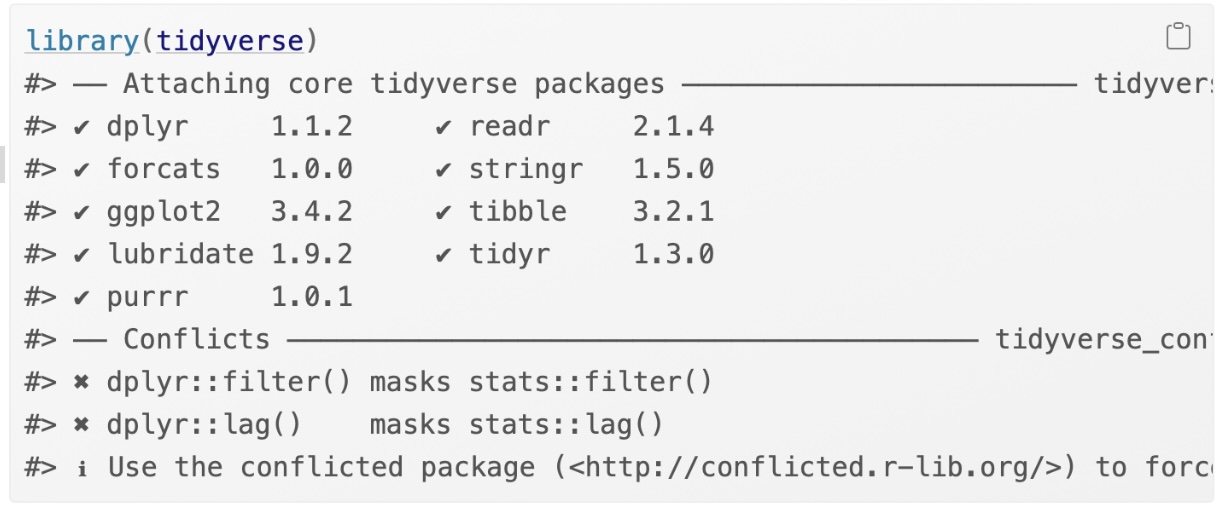
\includegraphics[width=0.75\textwidth,height=\textheight]{./images/Daily-2-Pic-1.jpg}

That one line of code loads the core tidyverse; packages which you will
use in almost every data analysis. It also tells you which functions
from the tidyverse conflict with functions in base R (or from other
packages you might have loaded).

If you run this code and get the error message ``\emph{there is no
package called `tidyverse'}'', you'll need to first install it, then run
\textbf{library()} once again.

You only need to install a package once, but you need to reload it every
time you start a new session. If we need to be explicit about where a
function (or dataset) comes from, we'll use the special form
\textbf{package::function()}. For example, \textbf{ggplot2::ggplot()}
tells you explicitly that we're using the \textbf{ggplot()} function
from the \textbf{ggplot2} package.

Let's use our first graph to answer a question: Do cars with big engines
use more fuel than cars with small engines? You probably already have an
answer, but try to make your answer precise. What does the relationship
between engine size and fuel efficiency look like?

You can test your answer with the mpg data frame found in ggplot2 (aka
\textbf{ggplot2::mpg}). A data frame is a rectangular collection of
variables (in the columns) and observations (in the rows). mpg contains
observations collected by the US Environmental Protection Agency on 38
models of car.

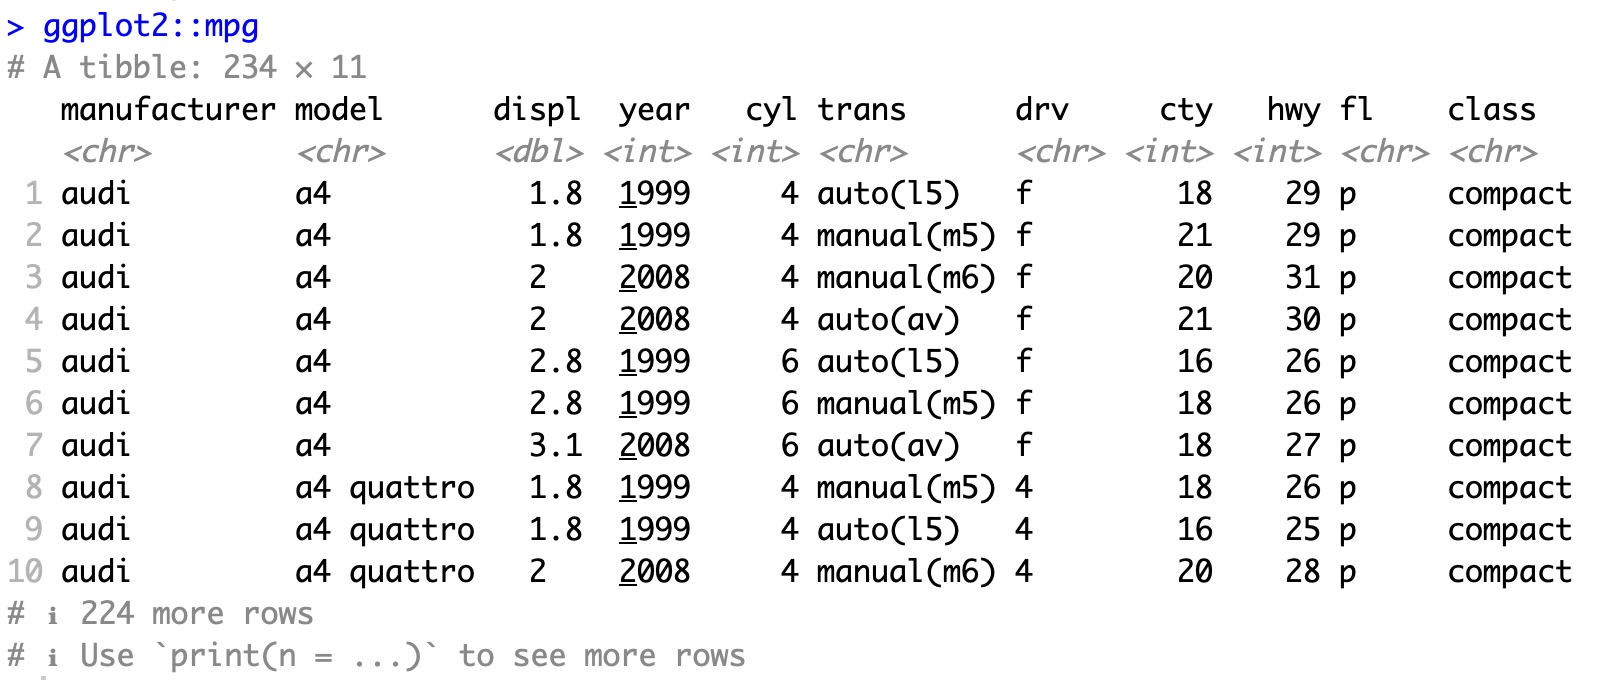
\includegraphics[width=0.75\textwidth,height=\textheight]{./images/Daily-2-Pic-2.jpg}

A few examples of the variables in \textbf{mpg} are:

\begin{enumerate}
\def\labelenumi{\arabic{enumi}.}
\item
  \textbf{displ}, a car's engine size, in litres.
\item
  \textbf{hwy}, a car's fuel efficiency on the highway, in miles per
  gallon (mpg). A car with a low fuel efficiency consumes more fuel than
  a car with a high fuel efficiency when they travel the same distance.
\end{enumerate}

To learn more about \textbf{mpg}, open its help page by running
\textbf{?mpg}.

To plot mpg, run this code to put \textbf{displ} on the x-axis and
\textbf{hwy} on the y-axis:

\begin{Shaded}
\begin{Highlighting}[]
\FunctionTok{library}\NormalTok{(tidyverse)}
\end{Highlighting}
\end{Shaded}

\begin{verbatim}
-- Attaching core tidyverse packages ------------------------ tidyverse 2.0.0 --
v dplyr     1.1.4     v readr     2.1.5
v forcats   1.0.0     v stringr   1.5.1
v ggplot2   3.5.1     v tibble    3.2.1
v lubridate 1.9.4     v tidyr     1.3.1
v purrr     1.0.2     
-- Conflicts ------------------------------------------ tidyverse_conflicts() --
x dplyr::filter() masks stats::filter()
x dplyr::lag()    masks stats::lag()
i Use the conflicted package (<http://conflicted.r-lib.org/>) to force all conflicts to become errors
\end{verbatim}

\begin{Shaded}
\begin{Highlighting}[]
\FunctionTok{ggplot}\NormalTok{(}\AttributeTok{data =}\NormalTok{ mpg) }\SpecialCharTok{+} 
  \FunctionTok{geom\_point}\NormalTok{(}\AttributeTok{mapping =} \FunctionTok{aes}\NormalTok{(}\AttributeTok{x =}\NormalTok{ displ, }\AttributeTok{y =}\NormalTok{ hwy))}
\end{Highlighting}
\end{Shaded}

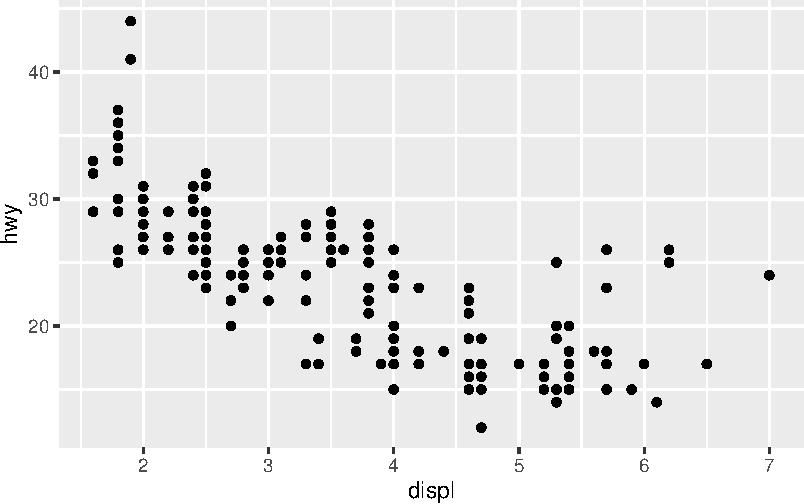
\includegraphics{Beginning_Data_Visualization_files/figure-pdf/Example1-1.pdf}

The plot shows a negative relationship between engine size (displ) and
fuel efficiency (hwy). In other words, cars with big engines use more
fuel. Does this confirm or refute your hypothesis about fuel efficiency
and engine size?

With ggplot2, you begin a plot with the function ggplot(). ggplot()
creates a coordinate system that you can add layers to. The first
argument of ggplot() is the dataset to use in the graph. So ggplot(data
= mpg) creates an empty graph, but it's not very interesting so I'm not
going to show it here.

You complete your graph by adding one or more layers to ggplot(). The
function geom\_point() adds a layer of points to your plot, which
creates a scatterplot. ggplot2 comes with many geom functions that each
add a different type of layer to a plot. You'll learn a whole bunch of
them throughout this section.

Each geom function in ggplot2 takes a mapping argument. This defines how
variables in your dataset are mapped to visual properties. The mapping
argument is always paired with aes(), and the x and y arguments of aes()
specify which variables to map to the x and y axes. ggplot2 looks for
the mapped variables in the data argument, in this case, mpg.

\subsection*{A Graphing Template}\label{a-graphing-template}
\addcontentsline{toc}{subsection}{A Graphing Template}

Let's turn this code into a reusable template for making graphs with
ggplot2. To make a graph, replace the bracketed sections in the code
below with a dataset, a geom function, or a collection of mappings.

\textbf{ggplot(data = \textless DATA\textgreater) +} \(\hspace{1in}\)
\textless GEOM\_FUNCTION\textgreater( mapping = aes(
\textless MAPPINGS\textgreater{} ) )

The rest of this assignment will show you how to complete and extend
this template to make different types of graphs. We will begin with the
\textbf{\textless MAPPINGS\textgreater{}} component.

\subsubsection*{Aesthetic Mappings}\label{aesthetic-mappings}
\addcontentsline{toc}{subsubsection}{Aesthetic Mappings}

``The greatest value of a picture is when it forces us to notice what we
never expected to see.'' --- John Tukey

In the plot below, one group of points (highlighted in red) seems to
fall outside of the linear trend. These cars have a higher mileage than
you might expect. How can you explain these cars?

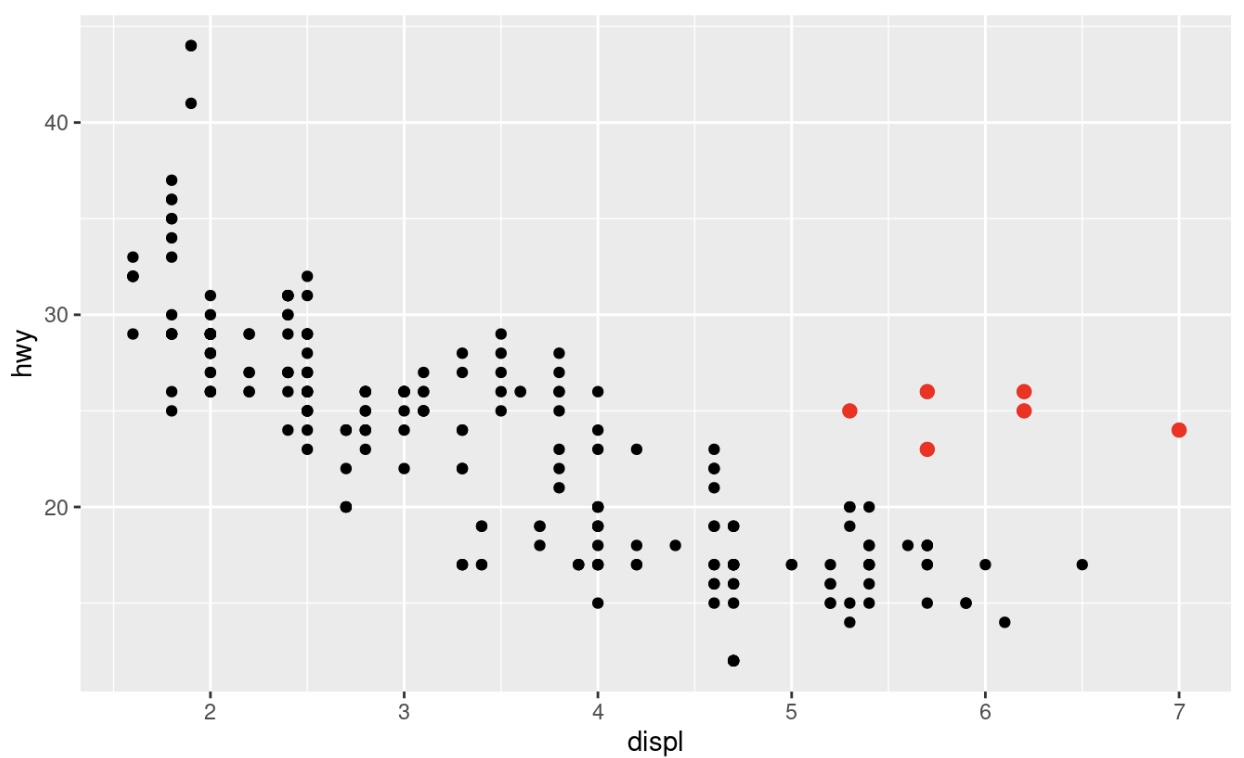
\includegraphics[width=0.75\textwidth,height=\textheight]{./images/Daily-2-Pic-3.jpg}

Let's hypothesize that the cars are hybrids. One way to test this
hypothesis is to look at the class value for each car. The class
variable of the mpg dataset classifies cars into groups such as compact,
midsize, and SUV. If the outlying points are hybrids, they should be
classified as compact cars or, perhaps, subcompact cars (keep in mind
that this data was collected before hybrid trucks and SUVs became
popular).

You can add a third variable, such as class, to a two dimensional
scatterplot by mapping it to an aesthetic. An aesthetic is a visual
property of the objects in your plot. Aesthetics include things like the
size, the shape, or the color of your points. You can display a point
(like the one below) in different ways by changing the values of its
aesthetic properties. Since we already use the word ``value'' to
describe data, let's use the word ``level'' to describe aesthetic
properties. Here we change the levels of a point's size, shape, and
color to make the point small, triangular, or blue:

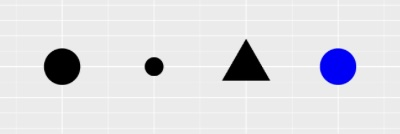
\includegraphics[width=0.35\textwidth,height=\textheight]{./images/Daily-2-Pic-4.jpg}

You can convey information about your data by mapping the aesthetics in
your plot to the variables in your dataset. For example, you can map the
colors of your points to the class variable to reveal the class of each
car.

\begin{Shaded}
\begin{Highlighting}[]
\FunctionTok{ggplot}\NormalTok{(}\AttributeTok{data =}\NormalTok{ mpg) }\SpecialCharTok{+}
  \FunctionTok{geom\_point}\NormalTok{(}\AttributeTok{mapping =} \FunctionTok{aes}\NormalTok{(}\AttributeTok{x =}\NormalTok{ displ, }\AttributeTok{y =}\NormalTok{ hwy, }\AttributeTok{color =}\NormalTok{ class))}
\end{Highlighting}
\end{Shaded}

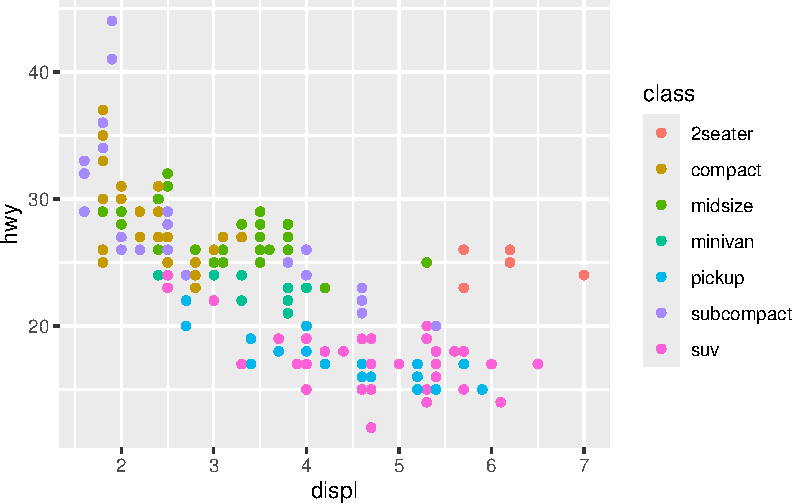
\includegraphics{Beginning_Data_Visualization_files/figure-pdf/Example-1.pdf}

(If you prefer British English, you can use colour instead of color.)

To map an aesthetic to a variable, associate the name of the aesthetic
to the name of the variable inside aes(). ggplot2 will automatically
assign a unique level of the aesthetic (here a unique color) to each
unique value of the variable, a process known as scaling. ggplot2 will
also add a legend that explains which levels correspond to which values.

The colors reveal that many of the unusual points are two-seater cars.
These cars don't seem like hybrids, and are, in fact, sports cars!
Sports cars have large engines like SUVs and pickup trucks, but small
bodies like midsize and compact cars, which improves their gas mileage.
In hindsight, these cars were unlikely to be hybrids since they have
large engines.

In the above example, we mapped class to the color aesthetic, but we
could have mapped class to the size aesthetic in the same way. In this
case, the exact size of each point would reveal its class affiliation.
We get a warning here, because mapping an unordered variable (class) to
an ordered aesthetic (size) is not a good idea.

\begin{Shaded}
\begin{Highlighting}[]
\FunctionTok{ggplot}\NormalTok{(}\AttributeTok{data =}\NormalTok{ mpg) }\SpecialCharTok{+}
  \FunctionTok{geom\_point}\NormalTok{(}\AttributeTok{mapping =} \FunctionTok{aes}\NormalTok{(}\AttributeTok{x =}\NormalTok{ displ, }\AttributeTok{y =}\NormalTok{ hwy, }\AttributeTok{size=}\NormalTok{class))}
\end{Highlighting}
\end{Shaded}

\begin{verbatim}
Warning: Using size for a discrete variable is not advised.
\end{verbatim}

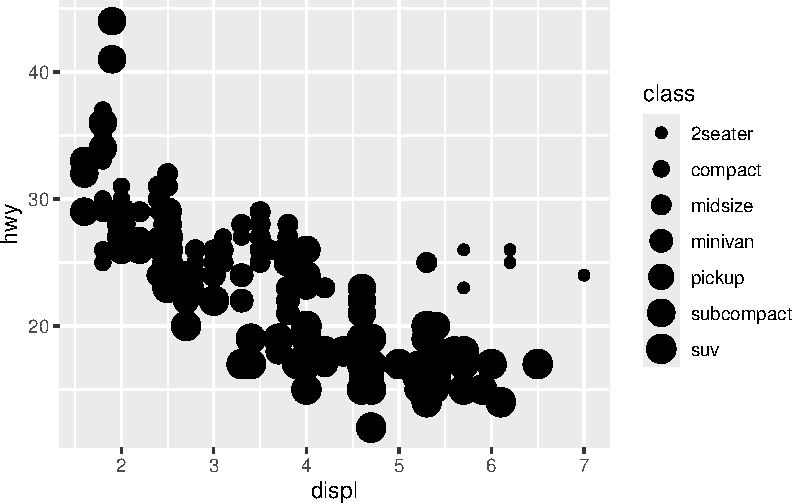
\includegraphics{Beginning_Data_Visualization_files/figure-pdf/Example2-1.pdf}

Or we could have mapped class to the alpha aesthetic, which controls the
transparency of the points, or to the shape aesthetic, which controls
the shape of the points.

\begin{Shaded}
\begin{Highlighting}[]
\FunctionTok{ggplot}\NormalTok{(}\AttributeTok{data=}\NormalTok{mpg) }\SpecialCharTok{+}
  \FunctionTok{geom\_point}\NormalTok{(}\AttributeTok{mapping =} \FunctionTok{aes}\NormalTok{(}\AttributeTok{x =}\NormalTok{ displ, }\AttributeTok{y =}\NormalTok{ hwy, }\AttributeTok{alpha =}\NormalTok{ class))}
\end{Highlighting}
\end{Shaded}

\begin{verbatim}
Warning: Using alpha for a discrete variable is not advised.
\end{verbatim}

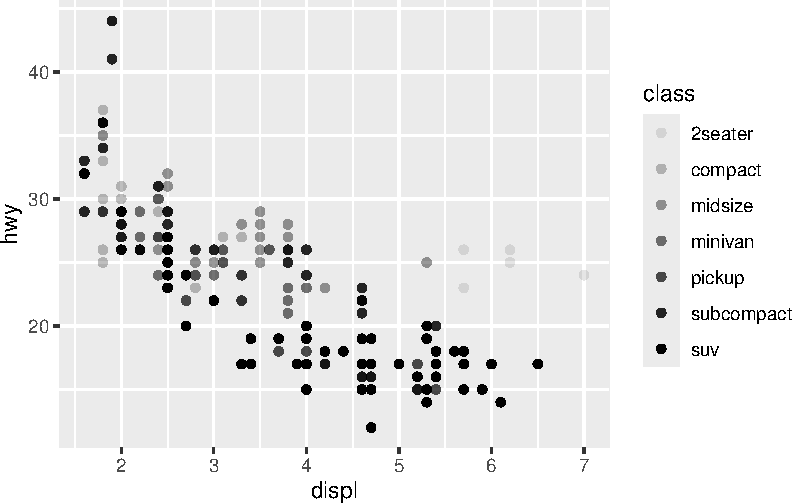
\includegraphics{Beginning_Data_Visualization_files/figure-pdf/Example 3-1.pdf}

\begin{Shaded}
\begin{Highlighting}[]
\FunctionTok{ggplot}\NormalTok{(}\AttributeTok{data =}\NormalTok{ mpg) }\SpecialCharTok{+} 
  \FunctionTok{geom\_point}\NormalTok{(}\AttributeTok{mapping =} \FunctionTok{aes}\NormalTok{(}\AttributeTok{x =}\NormalTok{ displ, }\AttributeTok{y =}\NormalTok{ hwy, }\AttributeTok{shape =}\NormalTok{ class))}
\end{Highlighting}
\end{Shaded}

\begin{verbatim}
Warning: The shape palette can deal with a maximum of 6 discrete values because more
than 6 becomes difficult to discriminate
i you have requested 7 values. Consider specifying shapes manually if you need
  that many have them.
\end{verbatim}

\begin{verbatim}
Warning: Removed 62 rows containing missing values or values outside the scale range
(`geom_point()`).
\end{verbatim}

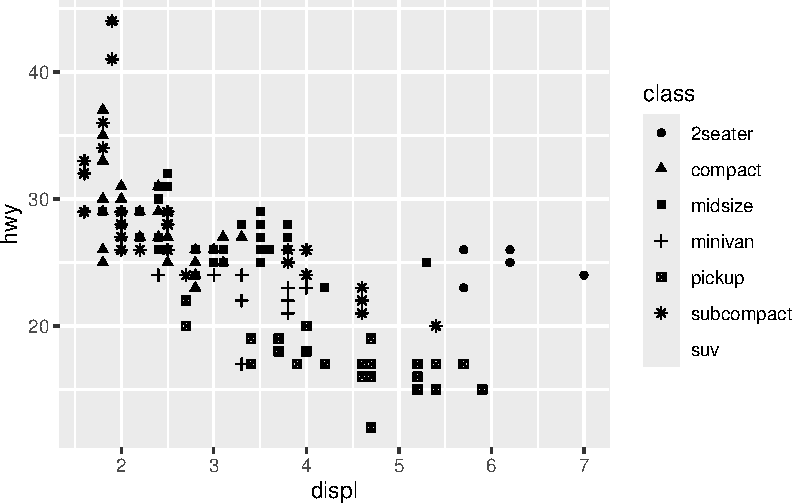
\includegraphics{Beginning_Data_Visualization_files/figure-pdf/Example 3-2.pdf}

What happened to the SUVs? ggplot2 will only use six shapes at a time.
By default, additional groups will go unplotted when you use the shape
aesthetic.

For each aesthetic, you use aes() to associate the name of the aesthetic
with a variable to display. The aes() function gathers together each of
the aesthetic mappings used by a layer and passes them to the layer's
mapping argument. The syntax highlights a useful insight about x and y:
the x and y locations of a point are themselves aesthetics, visual
properties that you can map to variables to display information about
the data.

Once you map an aesthetic, ggplot2 takes care of the rest. It selects a
reasonable scale to use with the aesthetic, and it constructs a legend
that explains the mapping between levels and values. For x and y
aesthetics, ggplot2 does not create a legend, but it creates an axis
line with tick marks and a label. The axis line acts as a legend; it
explains the mapping between locations and values.

You can also set the aesthetic properties of your geom manually. For
example, we can make all of the points in our plot blue:

\begin{Shaded}
\begin{Highlighting}[]
\FunctionTok{ggplot}\NormalTok{(}\AttributeTok{data =}\NormalTok{ mpg) }\SpecialCharTok{+} 
  \FunctionTok{geom\_point}\NormalTok{(}\AttributeTok{mapping =} \FunctionTok{aes}\NormalTok{(}\AttributeTok{x =}\NormalTok{ displ, }\AttributeTok{y =}\NormalTok{ hwy), }\AttributeTok{color =} \StringTok{"blue"}\NormalTok{)}
\end{Highlighting}
\end{Shaded}

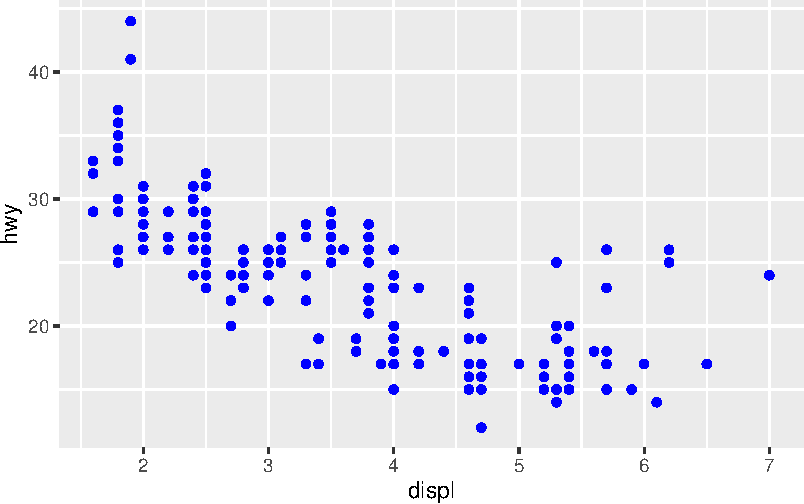
\includegraphics{Beginning_Data_Visualization_files/figure-pdf/Example 4-1.pdf}

Here, the color doesn't convey information about a variable, but only
changes the appearance of the plot. To set an aesthetic manually, set
the aesthetic by name as an argument of your geom function; i.e.~ it
goes outside of aes(). You'll need to pick a level that makes sense for
that aesthetic:

\begin{itemize}
\tightlist
\item
  name of a color as a character string.
\item
  The size of a point in mm.
\item
  The shape of a point as a number, as shown in Figure 3.1.
\end{itemize}

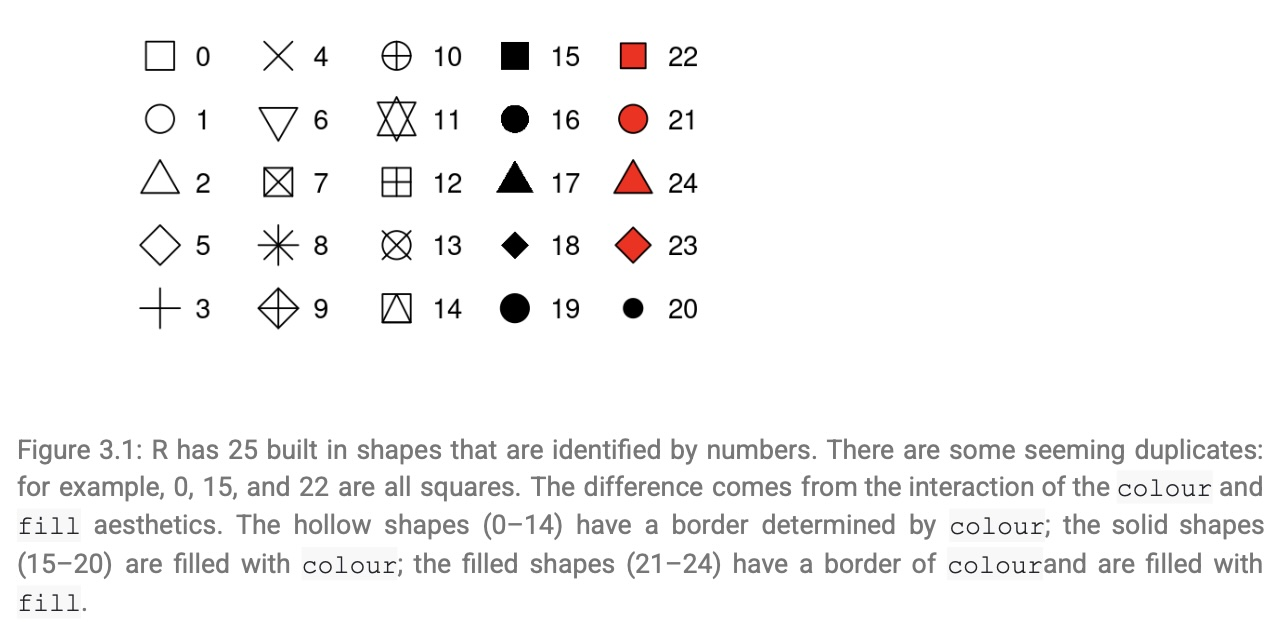
\includegraphics[width=0.75\textwidth,height=\textheight]{./images/Daily-2-Pic-5.jpg}

As you start to run R code, you're likely to run into problems. Don't
worry --- it happens to everyone.

Start by carefully comparing the code that you're running to the code in
the assignment. R is extremely picky, and a misplaced character can make
all the difference. Make sure that every ( is matched with a ) and every
'' is paired with another ``. Sometimes you'll run the code and nothing
happens. Check the left-hand of your console: if it's a +, it means that
R doesn't think you've typed a complete expression and it's waiting for
you to finish it. In this case, it's usually easy to start from scratch
again by pressing ESCAPE to abort processing the current command.

One common problem when creating ggplot2 graphics is to put the + in the
wrong place: it has to come at the end of the line, not the start. In
other words, make sure you haven't accidentally written code like this:

\begin{Shaded}
\begin{Highlighting}[]
\CommentTok{\# ggplot(data=mpg)}
\CommentTok{\# + geom\_point( mapping = aes(x = displ, y = hwy))}
\end{Highlighting}
\end{Shaded}

If you're still stuck, try the help. You can get help about any R
function by running ?function\_name in the console, or selecting the
function name and pressing F1 in RStudio. Don't worry if the help
doesn't seem that helpful - instead skip down to the examples and look
for code that matches what you're trying to do.

If that doesn't help, carefully read the error message. Sometimes the
answer will be buried there! But when you're new to R, the answer might
be in the error message but you don't yet know how to understand it.
Another great tool is Google: try googling the error message, as it's
likely someone else has had the same problem, and has gotten help
online.

\subsubsection*{Facets}\label{facets}
\addcontentsline{toc}{subsubsection}{Facets}

Reference : https://rpubs.com/uky994/583752

One way to add additional variables is with aesthetics. Another way,
particularly useful for categorical variables, is to split your plot
into facets, subplots that each display one subset of the data.

To facet your plot by a single variable, use facet\_wrap(). The first
argument of facet\_wrap() should be a formula, which you create with
\textasciitilde{} followed by a variable name (here ``formula'' is the
name of a data structure in R, not a synonym for ``equation''). The
variable that you pass to facet\_wrap() should be discrete.

\begin{Shaded}
\begin{Highlighting}[]
\FunctionTok{ggplot}\NormalTok{(}\AttributeTok{data =}\NormalTok{ mpg) }\SpecialCharTok{+} 
  \FunctionTok{geom\_point}\NormalTok{(}\AttributeTok{mapping =} \FunctionTok{aes}\NormalTok{(}\AttributeTok{x =}\NormalTok{ displ, }\AttributeTok{y =}\NormalTok{ hwy)) }\SpecialCharTok{+} 
  \FunctionTok{facet\_wrap}\NormalTok{(}\SpecialCharTok{\textasciitilde{}}\NormalTok{ class, }\AttributeTok{nrow =} \DecValTok{2}\NormalTok{)}
\end{Highlighting}
\end{Shaded}

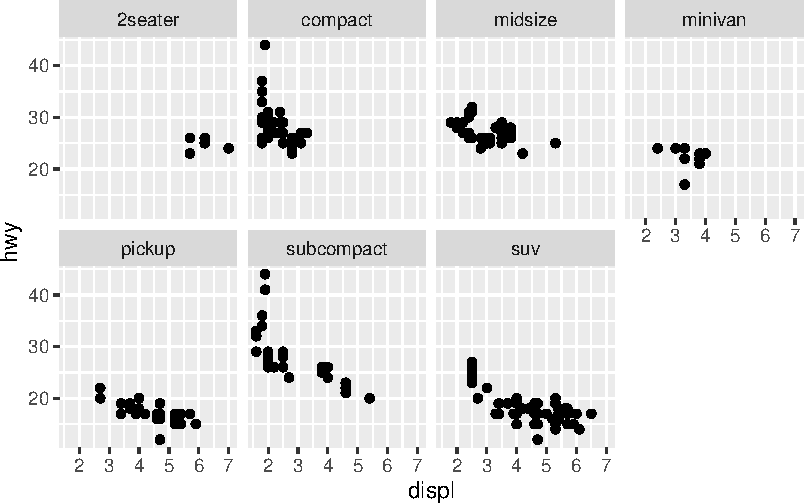
\includegraphics{Beginning_Data_Visualization_files/figure-pdf/Example 6-1.pdf}

To facet your plot on the combination of two variables, add
facet\_grid() to your plot call. The first argument of facet\_grid() is
also a formula. This time the formula should contain two variable names
separated by a \textasciitilde.

\begin{Shaded}
\begin{Highlighting}[]
\FunctionTok{ggplot}\NormalTok{(}\AttributeTok{data =}\NormalTok{ mpg) }\SpecialCharTok{+} 
  \FunctionTok{geom\_point}\NormalTok{(}\AttributeTok{mapping =} \FunctionTok{aes}\NormalTok{(}\AttributeTok{x =}\NormalTok{ displ, }\AttributeTok{y =}\NormalTok{ hwy)) }\SpecialCharTok{+} 
  \FunctionTok{facet\_grid}\NormalTok{(drv }\SpecialCharTok{\textasciitilde{}}\NormalTok{ cyl)}
\end{Highlighting}
\end{Shaded}

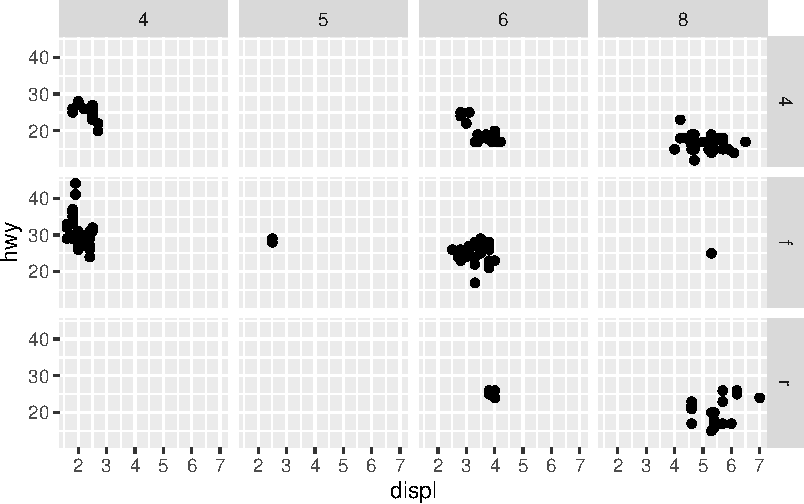
\includegraphics{Beginning_Data_Visualization_files/figure-pdf/Example 7-1.pdf}

If you prefer to not facet in the rows or columns dimension, use a \(.\)
(period) instead of a variable name, e.g.~

\(\hspace{1in}\) + facet\_grid( \textbf{.} \textasciitilde{} cyl).

\subsection*{Exercises}\label{exercises}
\addcontentsline{toc}{subsection}{Exercises}

\begin{enumerate}
\def\labelenumi{\arabic{enumi}.}
\tightlist
\item
  Run ggplot(data = mpg). What do you see? Why do you think this is?
\end{enumerate}

\begin{Shaded}
\begin{Highlighting}[]
\DocumentationTok{\#\#\# Write Code Here}

\CommentTok{\# ggplot(data = mpg)}
\end{Highlighting}
\end{Shaded}

2. How many rows are in mpg? How many columns?

\begin{Shaded}
\begin{Highlighting}[]
\DocumentationTok{\#\#\# Write Code Here}

\CommentTok{\# nrow(mpg)}

\CommentTok{\# ncol(mpg)}
\end{Highlighting}
\end{Shaded}

3. What does the drv variable describe? Read the help for ?mpg to find
out.

\begin{Shaded}
\begin{Highlighting}[]
\DocumentationTok{\#\#\# Write Code Here}
\end{Highlighting}
\end{Shaded}

4. Make a scatterplot of hwy vs cyl.

\begin{Shaded}
\begin{Highlighting}[]
\DocumentationTok{\#\#\# Write Code Here}

\CommentTok{\#ggplot(data = mpg, aes(x=hwy, y=cyl)) +}
\CommentTok{\#  geom\_point()}
\end{Highlighting}
\end{Shaded}

5. What happens if you make a scatterplot of class vs drv? Why is the
plot not useful?

\begin{Shaded}
\begin{Highlighting}[]
\DocumentationTok{\#\#\# Write Code Here}

\CommentTok{\#ggplot(data = mpg, aes(x=class, y=drv)) +}
\CommentTok{\#  geom\_point()}
\end{Highlighting}
\end{Shaded}

\begin{enumerate}
\def\labelenumi{\arabic{enumi}.}
\setcounter{enumi}{5}
\tightlist
\item
  Consider the following plot. Whay are the points not blue?
\end{enumerate}

\begin{Shaded}
\begin{Highlighting}[]
\FunctionTok{ggplot}\NormalTok{(}\AttributeTok{data =}\NormalTok{ mpg) }\SpecialCharTok{+} 
  \FunctionTok{geom\_point}\NormalTok{(}\AttributeTok{mapping =} \FunctionTok{aes}\NormalTok{(}\AttributeTok{x =}\NormalTok{ displ, }\AttributeTok{y =}\NormalTok{ hwy, }\AttributeTok{color =} \StringTok{"blue"}\NormalTok{))}
\end{Highlighting}
\end{Shaded}

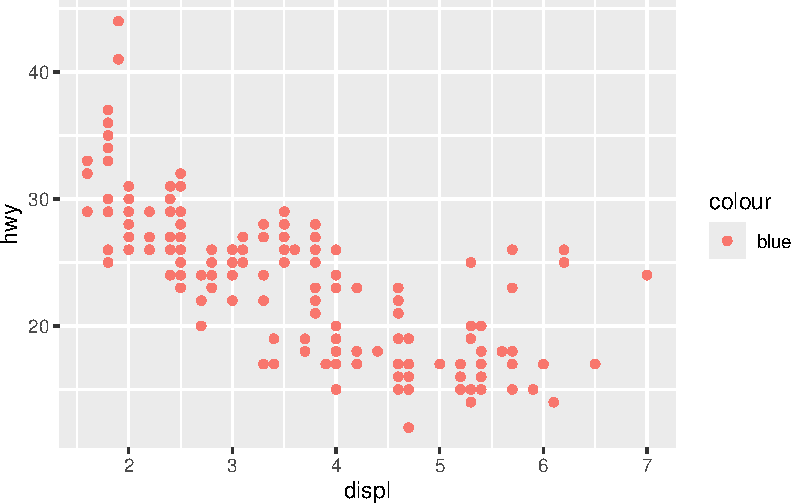
\includegraphics{Beginning_Data_Visualization_files/figure-pdf/Ex6-1.pdf}

\begin{enumerate}
\def\labelenumi{\arabic{enumi}.}
\setcounter{enumi}{6}
\tightlist
\item
  Which variables in mpg are categorical? Which variables are
  continuous? (Hint: type ?mpg to read the documentation for the
  dataset). How can you see this information when you run mpg?
\end{enumerate}

\begin{Shaded}
\begin{Highlighting}[]
\DocumentationTok{\#\#\# Answer}
\end{Highlighting}
\end{Shaded}

8. Map a continuous variable to color, size, and shape. How do these
aesthetics behave differently for categorical vs.~continuous variables?

\begin{Shaded}
\begin{Highlighting}[]
\DocumentationTok{\#\#\# Answer}
\end{Highlighting}
\end{Shaded}

9. What happens if you map the same variable to multiple aesthetics?

\begin{Shaded}
\begin{Highlighting}[]
\DocumentationTok{\#\#\# Answer}
\end{Highlighting}
\end{Shaded}

10. What does the \textbf{stroke} aesthetic do? What shapes does it work
with? (Hint: use ?geom\_point)

\begin{Shaded}
\begin{Highlighting}[]
\DocumentationTok{\#\#\# Answer}
\end{Highlighting}
\end{Shaded}

11. What happens if you map an aesthetic to something other than a
variable name, like aes(colour = displ \textless{} 5)? Note, you'll also
need to specify x and y.

\begin{Shaded}
\begin{Highlighting}[]
\DocumentationTok{\#\#\# Answer}
\end{Highlighting}
\end{Shaded}

\begin{enumerate}
\def\labelenumi{\arabic{enumi}.}
\setcounter{enumi}{11}
\tightlist
\item
  What happens if you facet on a continuous variable?
\end{enumerate}

\begin{Shaded}
\begin{Highlighting}[]
\CommentTok{\# Answer}
\end{Highlighting}
\end{Shaded}

13. What do the empty cells in plot with facet\_grid(drv
\textasciitilde{} cyl) mean? How do they relate to this plot?

\begin{Shaded}
\begin{Highlighting}[]
\FunctionTok{ggplot}\NormalTok{(}\AttributeTok{data =}\NormalTok{ mpg) }\SpecialCharTok{+} 
  \FunctionTok{geom\_point}\NormalTok{(}\AttributeTok{mapping =} \FunctionTok{aes}\NormalTok{(}\AttributeTok{x =}\NormalTok{ drv, }\AttributeTok{y =}\NormalTok{ cyl))}
\end{Highlighting}
\end{Shaded}

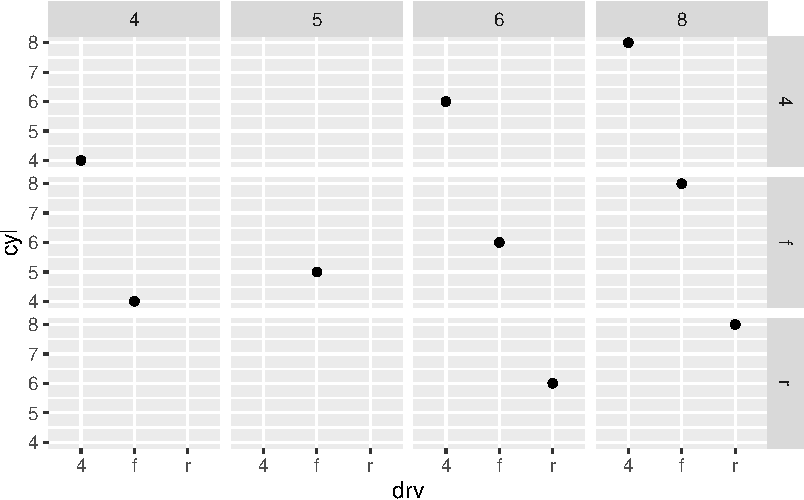
\includegraphics{Beginning_Data_Visualization_files/figure-pdf/Ex13-1.pdf}

14. What plots does the following code make? What does . do?

\begin{Shaded}
\begin{Highlighting}[]
\FunctionTok{ggplot}\NormalTok{(}\AttributeTok{data =}\NormalTok{ mpg) }\SpecialCharTok{+} 
  \FunctionTok{geom\_point}\NormalTok{(}\AttributeTok{mapping =} \FunctionTok{aes}\NormalTok{(}\AttributeTok{x =}\NormalTok{ displ, }\AttributeTok{y =}\NormalTok{ hwy)) }\SpecialCharTok{+}
  \FunctionTok{facet\_grid}\NormalTok{(drv }\SpecialCharTok{\textasciitilde{}}\NormalTok{ .)}
\end{Highlighting}
\end{Shaded}

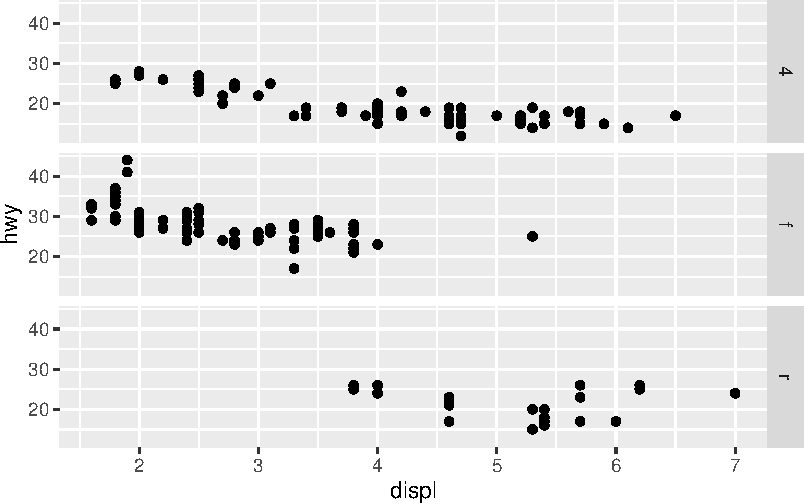
\includegraphics{Beginning_Data_Visualization_files/figure-pdf/Ex 14-1.pdf}

\begin{Shaded}
\begin{Highlighting}[]
\FunctionTok{ggplot}\NormalTok{(}\AttributeTok{data =}\NormalTok{ mpg) }\SpecialCharTok{+} 
  \FunctionTok{geom\_point}\NormalTok{(}\AttributeTok{mapping =} \FunctionTok{aes}\NormalTok{(}\AttributeTok{x =}\NormalTok{ displ, }\AttributeTok{y =}\NormalTok{ hwy)) }\SpecialCharTok{+}
 \FunctionTok{facet\_grid}\NormalTok{(. }\SpecialCharTok{\textasciitilde{}}\NormalTok{ cyl)}
\end{Highlighting}
\end{Shaded}

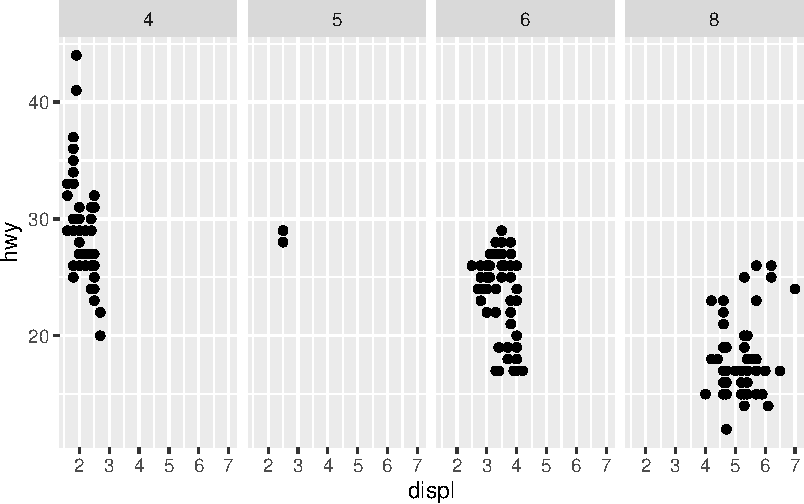
\includegraphics{Beginning_Data_Visualization_files/figure-pdf/Ex 14-2.pdf}

15. Consider the first faceted plot in this section. What are the
advantages to using faceting instead of the colour aesthetic? What are
the disadvantages? How might the balance change if you had a larger
dataset?

\begin{Shaded}
\begin{Highlighting}[]
\FunctionTok{ggplot}\NormalTok{(}\AttributeTok{data =}\NormalTok{ mpg) }\SpecialCharTok{+} 
  \FunctionTok{geom\_point}\NormalTok{(}\AttributeTok{mapping =} \FunctionTok{aes}\NormalTok{(}\AttributeTok{x =}\NormalTok{ displ, }\AttributeTok{y =}\NormalTok{ hwy)) }\SpecialCharTok{+} 
  \FunctionTok{facet\_wrap}\NormalTok{(}\SpecialCharTok{\textasciitilde{}}\NormalTok{ class, }\AttributeTok{nrow =} \DecValTok{2}\NormalTok{)}
\end{Highlighting}
\end{Shaded}

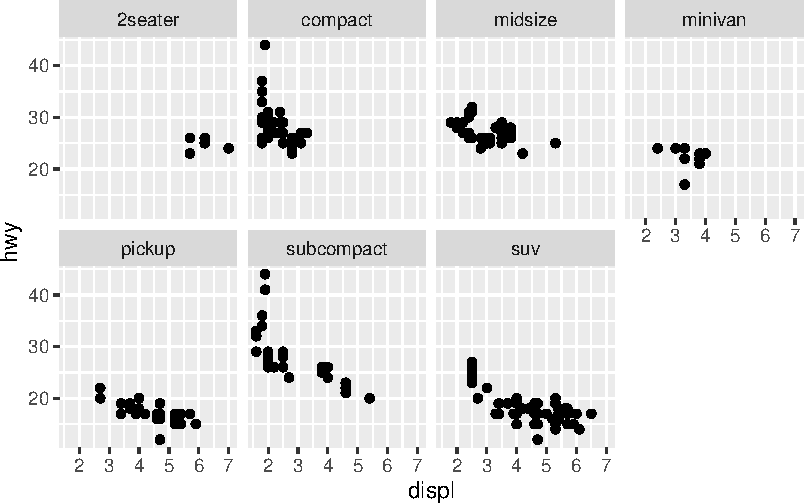
\includegraphics{Beginning_Data_Visualization_files/figure-pdf/Ex15-1.pdf}

16. Read \texttt{?facet\_wrap}. What does nrow do? What does ncol do?
What other options control the layout of the individual panels? Why
doesn't facet\_grid() have nrow and ncol arguments?

\begin{Shaded}
\begin{Highlighting}[]
\CommentTok{\# Answer}
\end{Highlighting}
\end{Shaded}

17. When using facet\_grid() you should usually put the variable with
more unique levels in the columns. Why?

\begin{Shaded}
\begin{Highlighting}[]
\CommentTok{\# Answer}
\end{Highlighting}
\end{Shaded}

Additional help : https://www.youtube.com/watch?v=HPJn1CMvtmI

\bookmarksetup{startatroot}

\chapter*{Reading In Data}\label{reading-in-data}
\addcontentsline{toc}{chapter}{Reading In Data}

\markboth{Reading In Data}{Reading In Data}

We have seen a few different ways for us to store data. We discussed
Vectors, Data Frames and Tibbles. We now move on to the question of how
we can get data from a file into R so we can start some Elementary Data
Analysis, Visualization, and other fun stuff!

\section*{CSV Files}\label{csv-files}
\addcontentsline{toc}{section}{CSV Files}

\markright{CSV Files}

Let's consider the case to where we have data in a CSV file. If you are
unaware, CSV stands for ``comma separated values.'' These are simple
text files where the data is separated by commas. We can use the
\texttt{read.csv()} or \texttt{read\_csv()}function to read the data
into a variable in R.

A CSV file can be upload to RStudio by clicking on ``File'' and then
``Import Dataset'' button and selecting ``From Text (base)'' or ``From
Text (readr).''

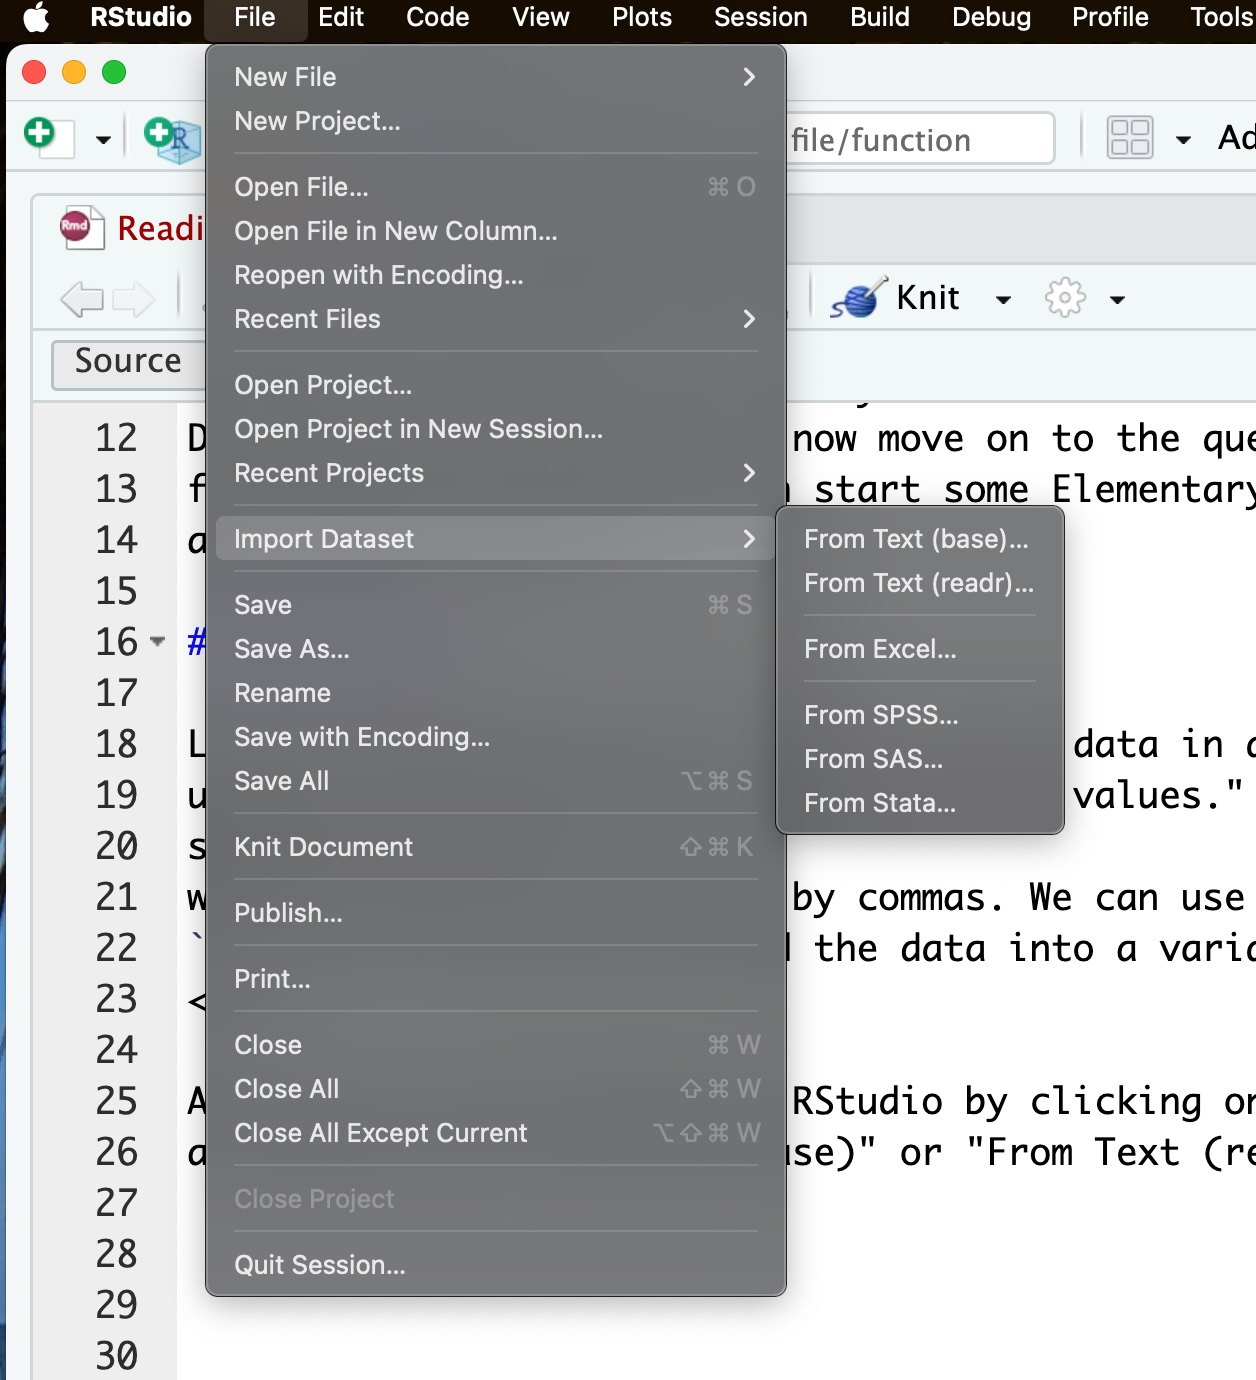
\includegraphics[width=0.6\textwidth,height=\textheight]{./images/Read-In-Data-1.jpg}

For this particular example, I asked ChatGPT to create a CSV file for me
using the following query :

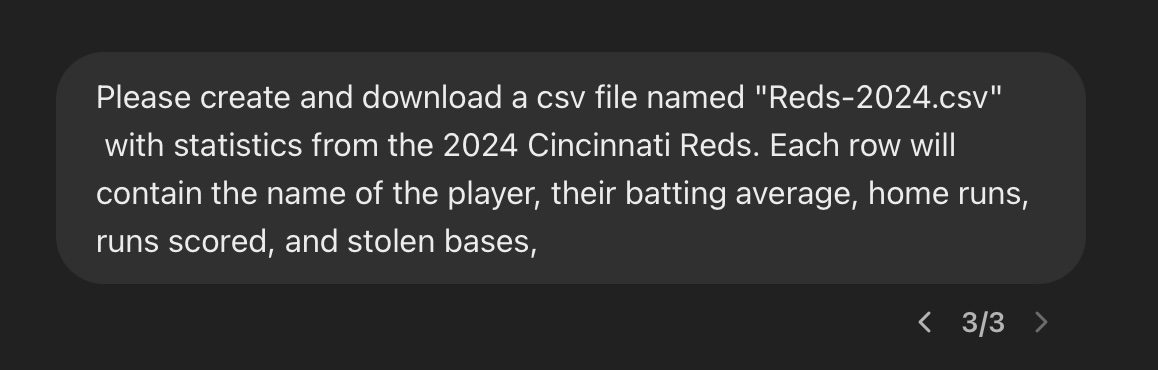
\includegraphics[width=0.6\textwidth,height=\textheight]{./images/Read-In-Data-6.jpg}

I then proceeded to upload it using the steps above. First, I went to
Files -\textgreater{} Import Dataset -\textgreater{} From Text (readr).
This gave me a new dialog and I clicked on the file \texttt{Reds-2024}.
Notice that I picked the CSV version and not the Pages version!

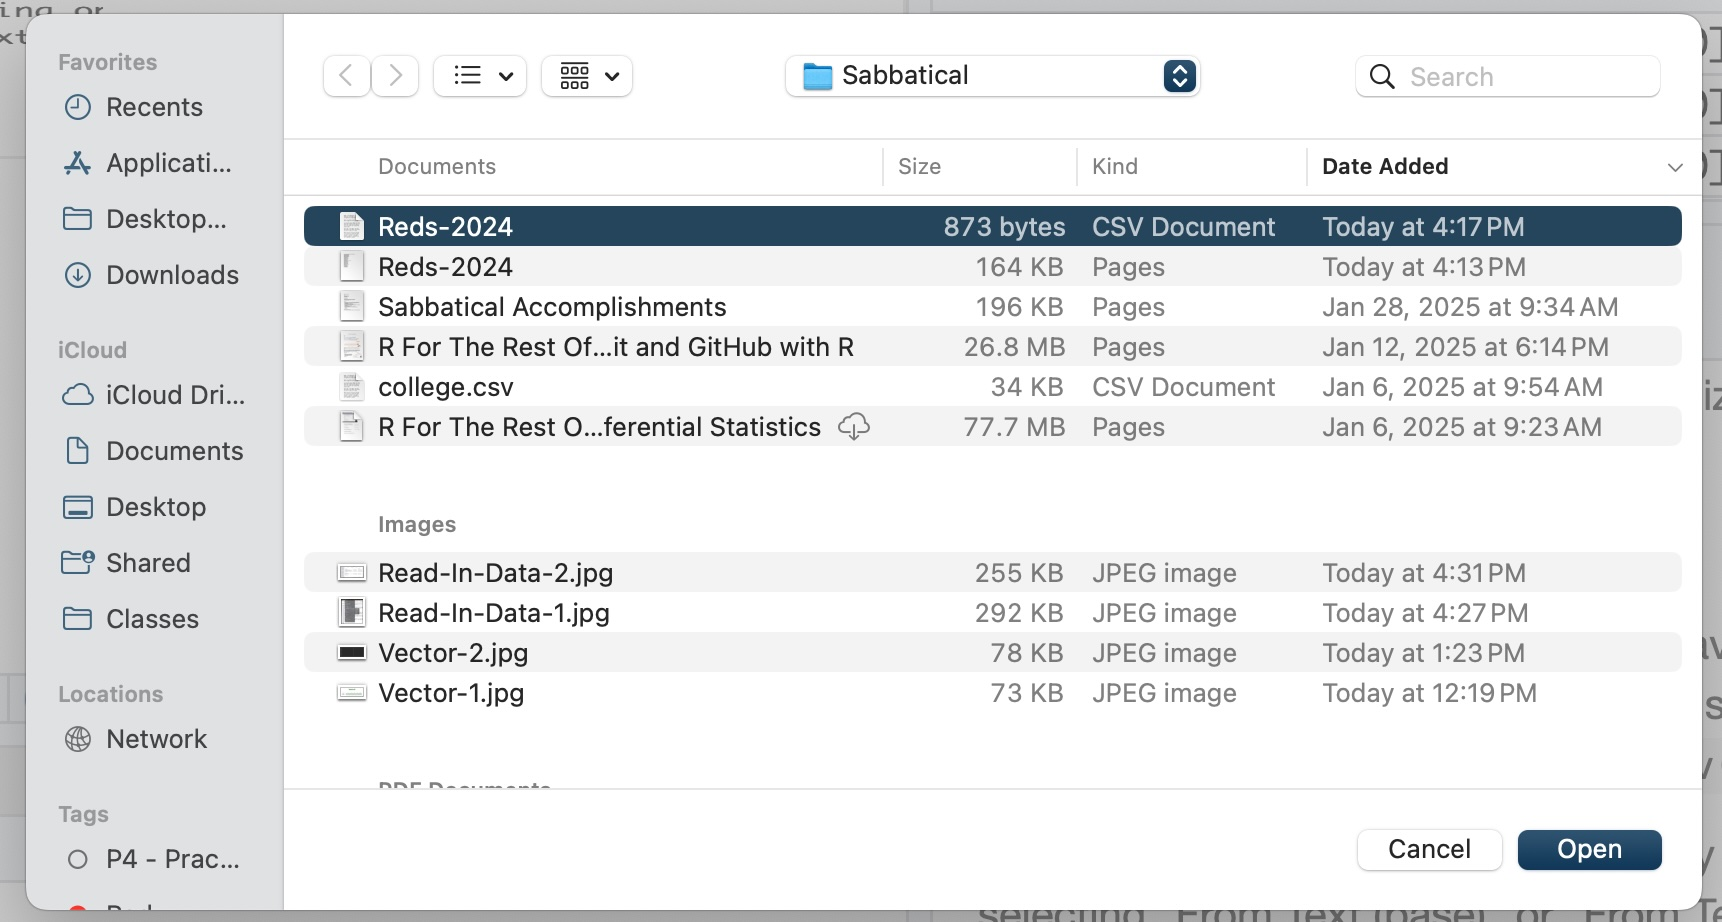
\includegraphics[width=0.6\textwidth,height=\textheight]{./images/Read-In-Data-3.jpg}

I then clicked on the ``Import'' button and a new dialog was presented
to me :

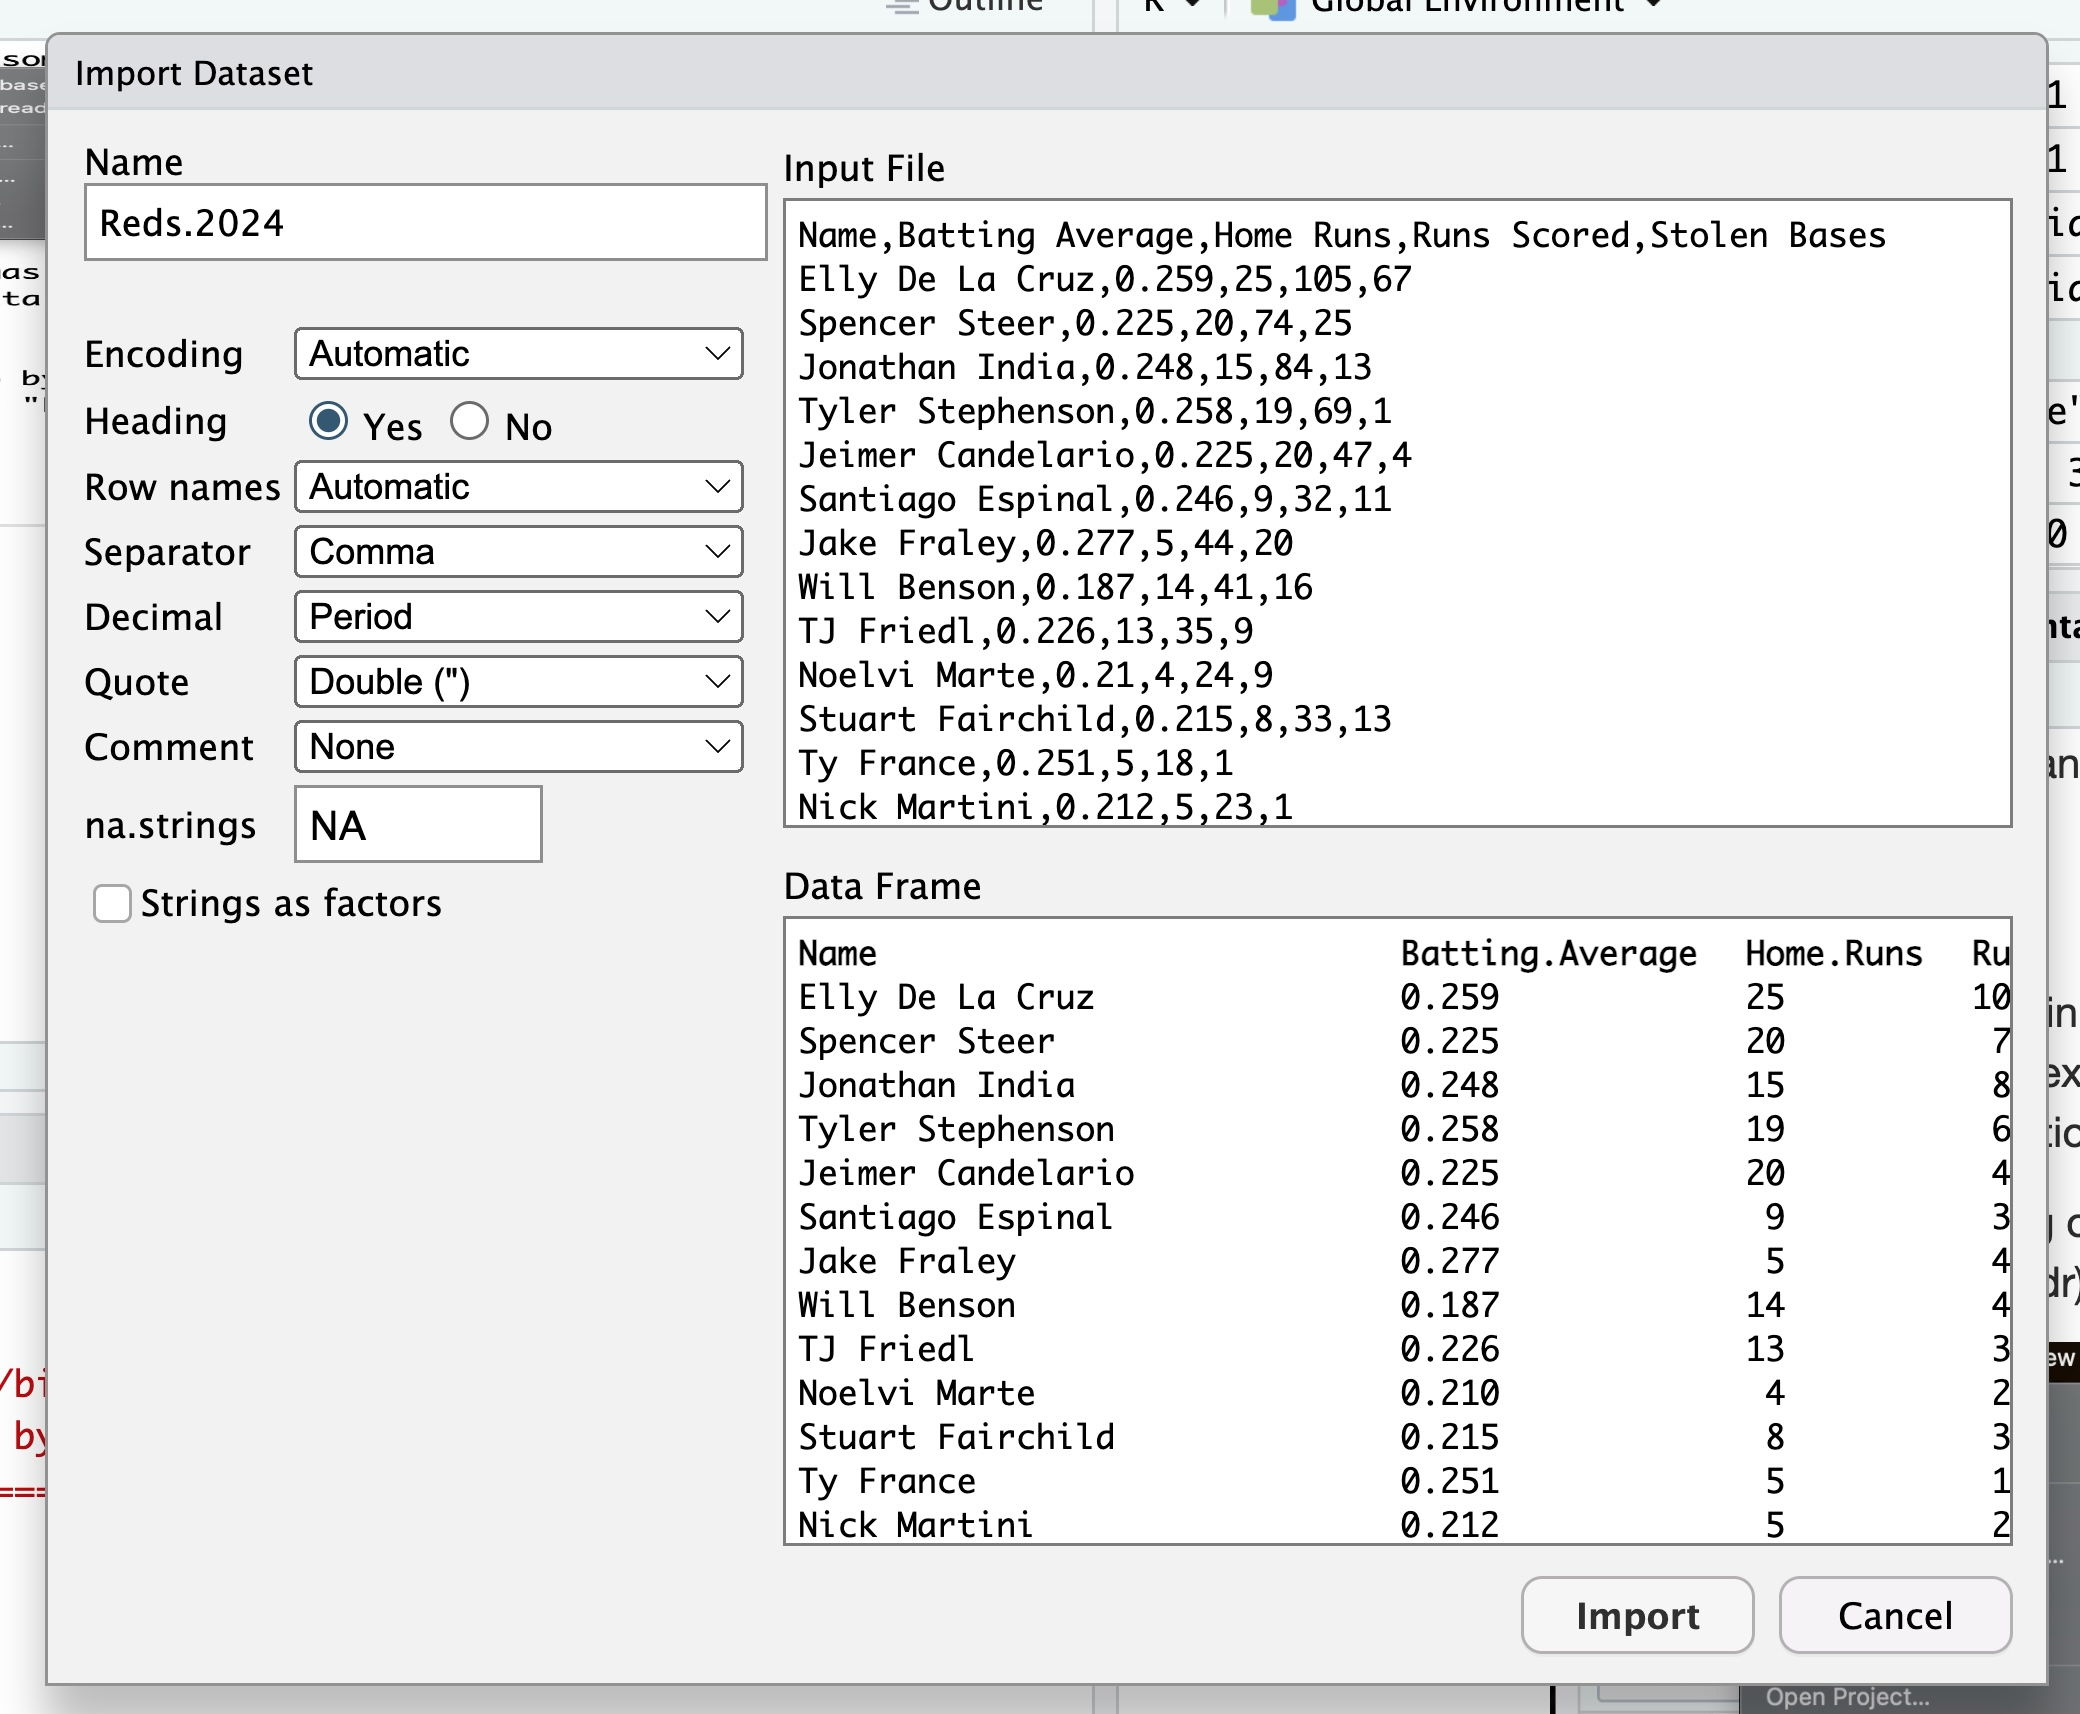
\includegraphics[width=0.6\textwidth,height=\textheight]{./images/Read-In-Data-4.jpg}

If you look in the upper left hand corner, you will see that you are
given a choice for the name of your file. The default one given is
\texttt{Reds.2024}, but you can change that to anything you wish. I went
ahead and just kept this default name. I clicked on the ``Import''
button and the data was loaded into RStudio into the variable
\texttt{Reds.2024}. You can look at the variable in the
\texttt{Environment} tab :

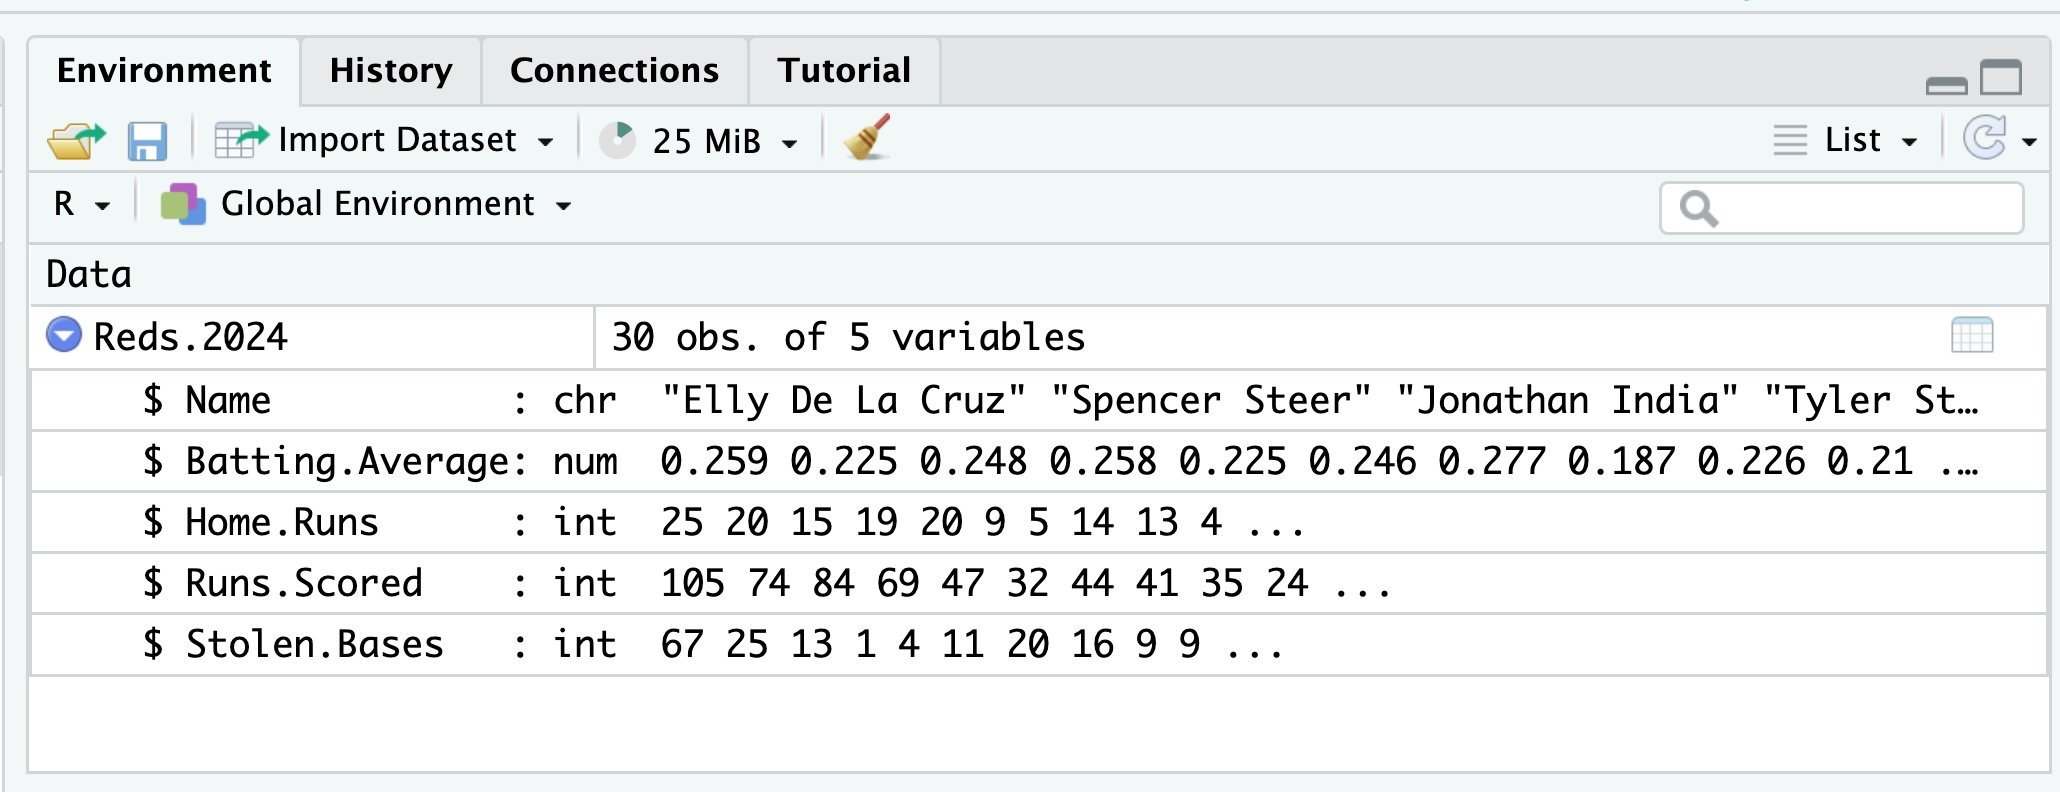
\includegraphics[width=0.6\textwidth,height=\textheight]{./images/Read-In-Data-7.jpg}

You can also see the CSV file in the \texttt{Files} tab :

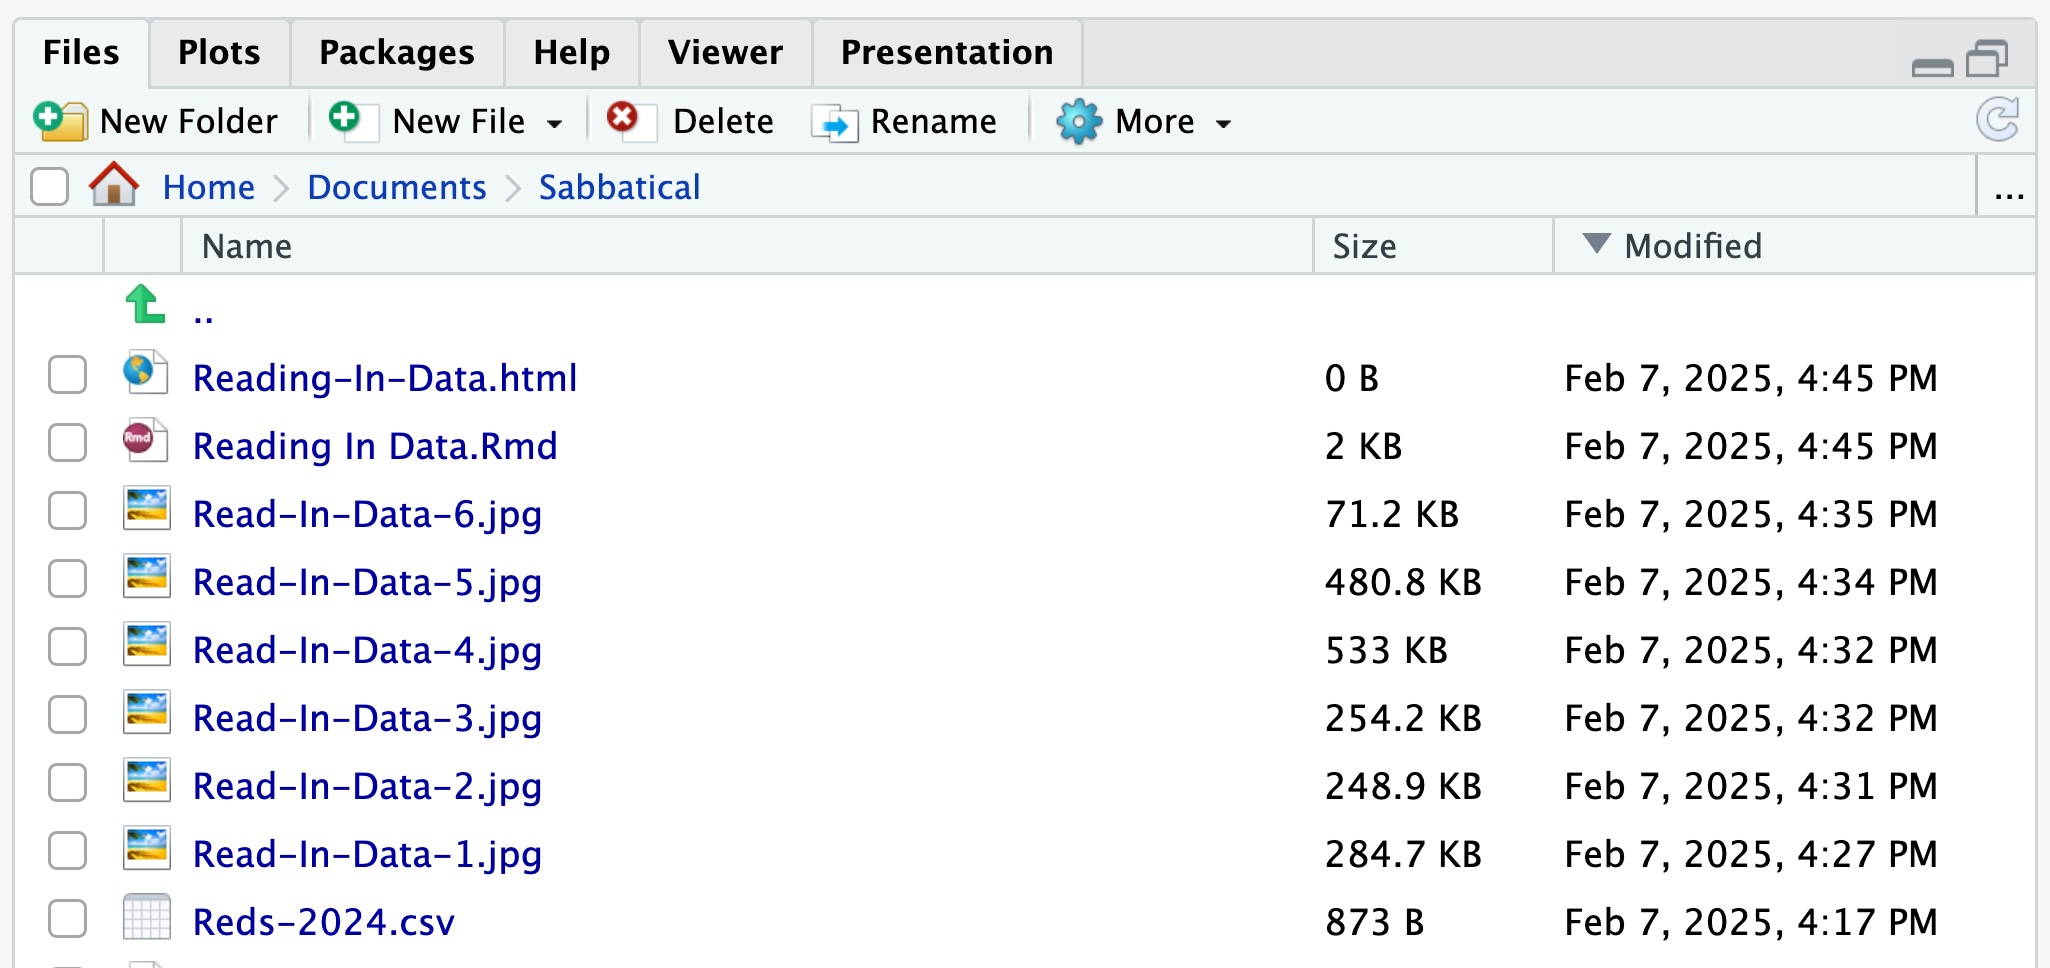
\includegraphics[width=0.6\textwidth,height=\textheight]{./images/Read-In-Data-8.jpg}

\subsection*{read.csv( )}\label{read.csv}
\addcontentsline{toc}{subsection}{read.csv( )}

We can write part of our code to read in a CSV file using the
\texttt{read.csv()} function. The \texttt{read.csv()} function takes in
a file path as an argument. If you have a CSV file uploaded into the
files section of RStudio, you can use the \texttt{read.csv()} function :

\begin{Shaded}
\begin{Highlighting}[]
\CommentTok{\# Read in the data}

\NormalTok{Reds2024\_Another\_Version }\OtherTok{\textless{}{-}} \FunctionTok{read.csv}\NormalTok{(}\StringTok{"./Reds{-}2024.csv"}\NormalTok{)}

\CommentTok{\# }\AlertTok{CAUTION}\CommentTok{ : When creating variable names to use in your R script,}
\CommentTok{\# make sure you use an underscore and not a dash. When R sees a dash, }
\CommentTok{\# it can sometimes be interpreted as a minus sign and not a dash. }
\CommentTok{\# This can cause errors in your code.}

\CommentTok{\# You can try this by removing the comment tag below :}

\CommentTok{\# Reds{-}2024 \textless{}{-} read.csv("Reds{-}2024.csv")}
\end{Highlighting}
\end{Shaded}

We can now see the new version of the data in the \texttt{Environment}
tab :

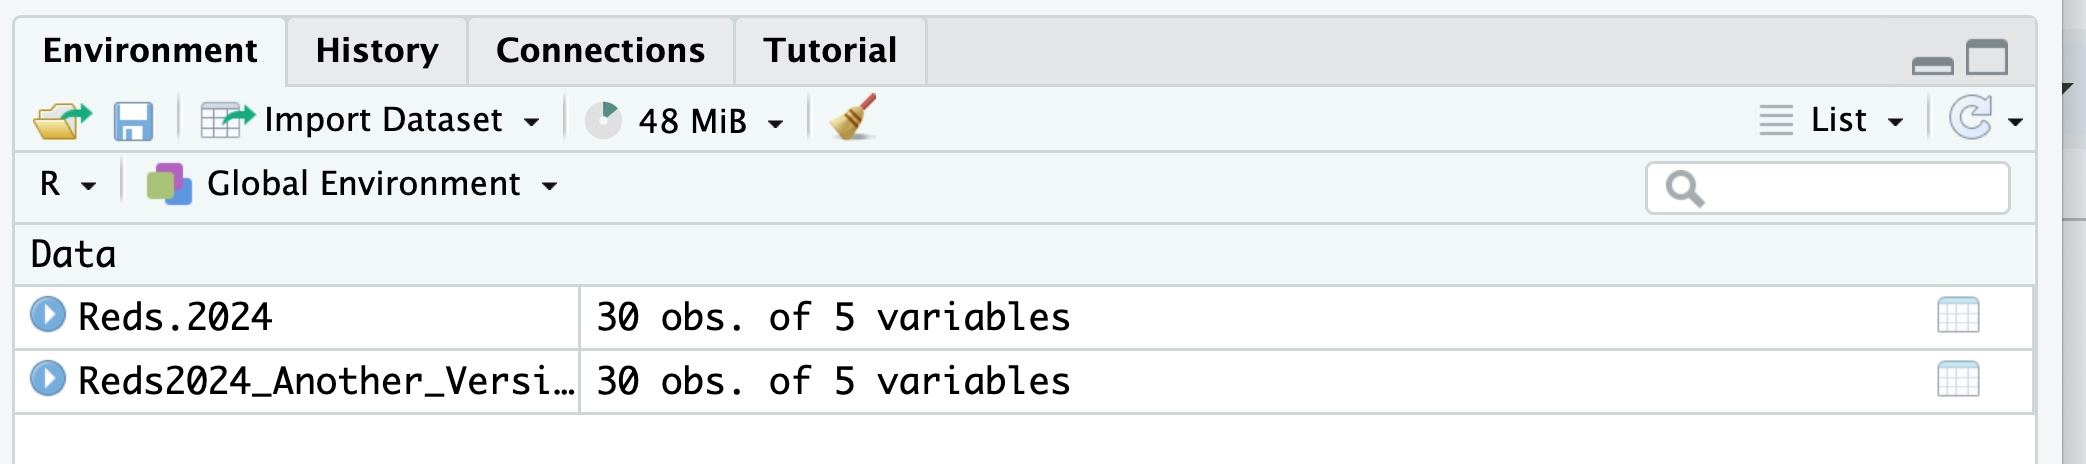
\includegraphics[width=0.6\textwidth,height=\textheight]{./images/Read-In-Data-9.jpg}

\texttt{read.csv()} is a base R function. That means it is already
loaded up when you start RStudio. You do not need to load any packages
to use it.

However, there is a more powerful function called \texttt{read\_csv()}
that is part of the \texttt{readr} package. It can read in data faster
and it can also read in data that is not in a CSV format, but we will
stick with the CSV format for now.

\subsection*{read\_csv( )}\label{read_csv}
\addcontentsline{toc}{subsection}{read\_csv( )}

One of the differences between read.csv( ) and read\_csv( ) is that
read\_csv( ) is part of the \texttt{readr} package. This means you will
need to load the \texttt{readr} package to use it. This is part of the
\texttt{tidyverse} package. If you do not have tidyverse installed, make
sure you go ahead and install it. Once tidyverse is install, you can
load up the \texttt{readr} package.

If you are unsure if the \texttt{readr} package is loaded, you can look
at the \texttt{Packages} tab in RStudio to see if the \texttt{readr}
package is loaded. If it is not, you can load it by clicking on the
checkbox next to the package name.

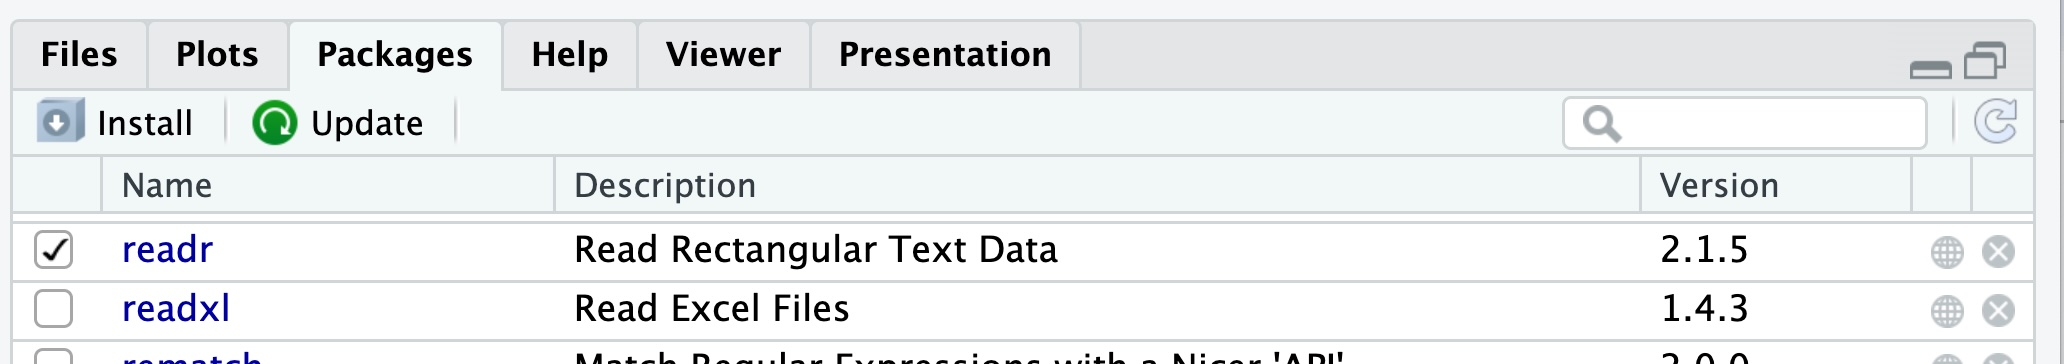
\includegraphics[width=0.6\textwidth,height=\textheight]{./images/Read-In-Data-10.jpg}

If needed, you can also put this into your script so the user will have
it loaded up for them. You can load the \texttt{readr} package by using
the \texttt{library()} function :

\begin{Shaded}
\begin{Highlighting}[]
\CommentTok{\# Load the readr package}

\FunctionTok{library}\NormalTok{(readr)}
\end{Highlighting}
\end{Shaded}

You can now use the \texttt{read\_csv()} function to read in the data :

\begin{Shaded}
\begin{Highlighting}[]
\CommentTok{\# Read in the data}

\NormalTok{Reds2024\_Version\_3 }\OtherTok{\textless{}{-}} \FunctionTok{read\_csv}\NormalTok{(}\StringTok{"Reds{-}2024.csv"}\NormalTok{)}
\end{Highlighting}
\end{Shaded}

\begin{verbatim}
Rows: 30 Columns: 5
-- Column specification --------------------------------------------------------
Delimiter: ","
chr (1): Name
dbl (4): Batting Average, Home Runs, Runs Scored, Stolen Bases

i Use `spec()` to retrieve the full column specification for this data.
i Specify the column types or set `show_col_types = FALSE` to quiet this message.
\end{verbatim}

Why is read\_csv better than read.csv? It is faster and it can read in
data that is not in a CSV format. It can read in data that is in a TSV
(Tab Separated Value) format, a DSV (Delimiter Separated Value) format,
and a few others. It can also read in data that is in a fixed width
format.

Basically, when in doubt, use \texttt{read\_csv(\ )} instead of
\texttt{read.csv(\ )}.

Now that we have the data loaded into R, we can start to do some
Elementary Data Analysis. We can use all the commands we discussed when
going over Vectors, Data Frames, and Tibbles.

\begin{Shaded}
\begin{Highlighting}[]
\CommentTok{\# Look at the data}

\FunctionTok{head}\NormalTok{(Reds2024\_Version\_3)}
\end{Highlighting}
\end{Shaded}

\begin{verbatim}
# A tibble: 6 x 5
  Name              `Batting Average` `Home Runs` `Runs Scored` `Stolen Bases`
  <chr>                         <dbl>       <dbl>         <dbl>          <dbl>
1 Elly De La Cruz               0.259          25           105             67
2 Spencer Steer                 0.225          20            74             25
3 Jonathan India                0.248          15            84             13
4 Tyler Stephenson              0.258          19            69              1
5 Jeimer Candelario             0.225          20            47              4
6 Santiago Espinal              0.246           9            32             11
\end{verbatim}

\begin{Shaded}
\begin{Highlighting}[]
\CommentTok{\# Look at the structure of the data}

\FunctionTok{class}\NormalTok{(Reds2024\_Version\_3)}
\end{Highlighting}
\end{Shaded}

\begin{verbatim}
[1] "spec_tbl_df" "tbl_df"      "tbl"         "data.frame" 
\end{verbatim}

\begin{Shaded}
\begin{Highlighting}[]
\CommentTok{\# Look at the Stolen Bases category }

\NormalTok{Reds2024\_Version\_3}\SpecialCharTok{$}\StringTok{\textasciigrave{}}\AttributeTok{Stolen Bases}\StringTok{\textasciigrave{}}
\end{Highlighting}
\end{Shaded}

\begin{verbatim}
 [1] 67 25 13  1  4 11 20 16  9  9 13  1  1  2  0  0  3  2  2  2  0  0  0  5  0
[26]  0  1  0  0  0
\end{verbatim}

\subsection*{Using URL's}\label{using-urls}
\addcontentsline{toc}{subsection}{Using URL's}

You can also read in data from a URL. This is useful if you have a CSV
file hosted on a website. You can use the \texttt{read.csv()} os
\texttt{read\_csv()} functions to read in the data from the URL.

If there is a direct URL to a CSV sheet, then you can use one of these
commands to read in the data :

\begin{Shaded}
\begin{Highlighting}[]
\CommentTok{\# data\_name \textless{}{-} read.csv(\textquotesingle{}URL\textquotesingle{})}

\NormalTok{data1 }\OtherTok{\textless{}{-}} \FunctionTok{read.csv}\NormalTok{(}\StringTok{\textquotesingle{}https://www.stats.govt.nz/assets/Uploads/Annual{-}enterprise{-}survey/Annual{-}enterprise{-}survey{-}2020{-}financial{-}year{-}provisional/Download{-}data/annual{-}enterprise{-}survey{-}2020{-}financial{-}year{-}provisional{-}csv.csv\textquotesingle{}}\NormalTok{)}

\FunctionTok{head}\NormalTok{(data1,}\DecValTok{2}\NormalTok{)}
\end{Highlighting}
\end{Shaded}

\begin{verbatim}
  Year Industry_aggregation_NZSIOC Industry_code_NZSIOC Industry_name_NZSIOC
1 2020                     Level 1                99999       All industries
2 2020                     Level 1                99999       All industries
               Units Variable_code
1 Dollars (millions)           H01
2 Dollars (millions)           H04
                                    Variable_name     Variable_category   Value
1                                    Total income Financial performance 733,258
2 Sales, government funding, grants and subsidies Financial performance 660,630
                                                                                            Industry_code_ANZSIC06
1 ANZSIC06 divisions A-S (excluding classes K6330, L6711, O7552, O760, O771, O772, S9540, S9601, S9602, and S9603)
2 ANZSIC06 divisions A-S (excluding classes K6330, L6711, O7552, O760, O771, O772, S9540, S9601, S9602, and S9603)
\end{verbatim}

\begin{Shaded}
\begin{Highlighting}[]
\CommentTok{\# data\_name \textless{}{-} read\_csv(\textquotesingle{}URL\textquotesingle{})}
\NormalTok{data2 }\OtherTok{\textless{}{-}} \FunctionTok{read\_csv}\NormalTok{(}\StringTok{\textquotesingle{}https://www.stats.govt.nz/assets/Uploads/Annual{-}enterprise{-}survey/Annual{-}enterprise{-}survey{-}2020{-}financial{-}year{-}provisional/Download{-}data/annual{-}enterprise{-}survey{-}2020{-}financial{-}year{-}provisional{-}csv.csv\textquotesingle{}}\NormalTok{)}
\end{Highlighting}
\end{Shaded}

\begin{verbatim}
Rows: 37080 Columns: 10
-- Column specification --------------------------------------------------------
Delimiter: ","
chr (9): Industry_aggregation_NZSIOC, Industry_code_NZSIOC, Industry_name_NZ...
dbl (1): Year

i Use `spec()` to retrieve the full column specification for this data.
i Specify the column types or set `show_col_types = FALSE` to quiet this message.
\end{verbatim}

\begin{Shaded}
\begin{Highlighting}[]
\FunctionTok{head}\NormalTok{(data2,}\DecValTok{2}\NormalTok{)}
\end{Highlighting}
\end{Shaded}

\begin{verbatim}
# A tibble: 2 x 10
   Year Industry_aggregation_N~1 Industry_code_NZSIOC Industry_name_NZSIOC Units
  <dbl> <chr>                    <chr>                <chr>                <chr>
1  2020 Level 1                  99999                All industries       Doll~
2  2020 Level 1                  99999                All industries       Doll~
# i abbreviated name: 1: Industry_aggregation_NZSIOC
# i 5 more variables: Variable_code <chr>, Variable_name <chr>,
#   Variable_category <chr>, Value <chr>, Industry_code_ANZSIC06 <chr>
\end{verbatim}

Note : As of now, there is not an easy way to read in data from a Google
Drive. You can try to use the \texttt{googledrive} package, but for our
purposes, if we have a csv file on Google Drive, we will download the
file and upload it as we did earlier.

\section*{Excel Files}\label{excel-files}
\addcontentsline{toc}{section}{Excel Files}

\markright{Excel Files}

We can also read in data from an Excel file. We can use the
\texttt{readxl} package to read in the data. If you do not have the
\texttt{readxl} package installed, you can install it by using the
\texttt{install.packages()} function :

\begin{Shaded}
\begin{Highlighting}[]
\CommentTok{\# Install the readxl package}

\CommentTok{\# install.packages("readxl")}
\end{Highlighting}
\end{Shaded}

You can then load the \texttt{readxl} package by using the
\texttt{library()} function :

\begin{Shaded}
\begin{Highlighting}[]
\CommentTok{\# Load the readxl package}

\FunctionTok{library}\NormalTok{(readxl)}
\end{Highlighting}
\end{Shaded}

You can then use the \texttt{read\_excel()} function to read in the data
:

\begin{Shaded}
\begin{Highlighting}[]
\CommentTok{\# Read in the data}

\NormalTok{data3 }\OtherTok{\textless{}{-}} \FunctionTok{read\_excel}\NormalTok{(}\StringTok{"Reds\_1\_Excel.xlsx"}\NormalTok{)}

\FunctionTok{head}\NormalTok{(data3,}\DecValTok{2}\NormalTok{)}
\end{Highlighting}
\end{Shaded}

\begin{verbatim}
# A tibble: 2 x 5
  Name            `Batting Average` `Home Runs` `Runs Scored` `Stolen Bases`
  <chr>                       <dbl>       <dbl>         <dbl>          <dbl>
1 Elly De La Cruz             0.259          25           105             67
2 Spencer Steer               0.225          20            74             25
\end{verbatim}

This allows to now carry out some EDA on the variable \texttt{data3}.
For example, if we wanted to sum up the number of home runs hit by the
Reds in 2024, we could use the following code :

\begin{Shaded}
\begin{Highlighting}[]
\CommentTok{\# Sum up the number of home runs hit by the Reds in 2024}

\FunctionTok{sum}\NormalTok{(data3}\SpecialCharTok{$}\StringTok{\textasciigrave{}}\AttributeTok{Home Runs}\StringTok{\textasciigrave{}}\NormalTok{)}
\end{Highlighting}
\end{Shaded}

\begin{verbatim}
[1] 174
\end{verbatim}

\bookmarksetup{startatroot}

\chapter*{Vectors, Data Frames,
Tibbles}\label{vectors-data-frames-tibbles}
\addcontentsline{toc}{chapter}{Vectors, Data Frames, Tibbles}

\markboth{Vectors, Data Frames, Tibbles}{Vectors, Data Frames, Tibbles}

Let's talk a little bit about structures we can use to store data. These
can be complex, so we will just talk about some basic ways in which we
will be using them.

\section*{Vectors}\label{vectors}
\addcontentsline{toc}{section}{Vectors}

\markright{Vectors}

A vector is a 1-dimensional (row) structure that can hold multiple
elements. For example, we can create a vector that contains 10 numbers
such as this one :

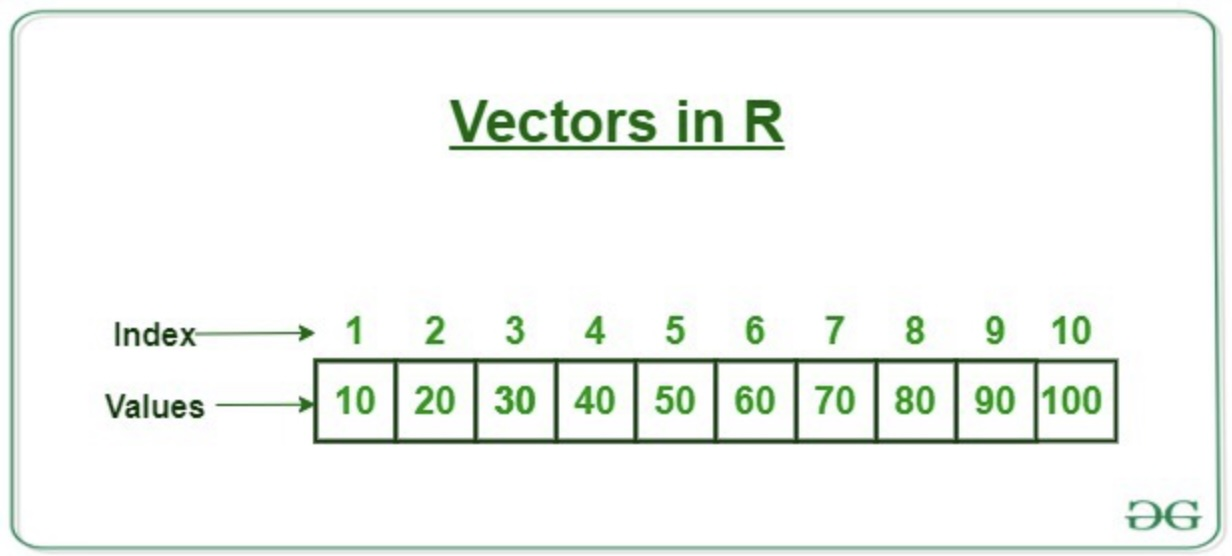
\includegraphics[width=0.6\textwidth,height=\textheight]{./images/Vector-1.jpg}

This example is a 1-dimensional vector that holds 10 values. You can see
the \textbf{values} that we have saved are 10, 20, 30, 40, 50, 60, 70,
80, 90, and 100. The \textbf{index} tells us what position each value is
in. The first value is at index 1, the second value is at index 2, and
so on.

When creating a new vector, you want to make sure you are giving it a
name that makes sense. For example, if you are creating a vector that
holds the scores from a test, you might want to name it
\texttt{test\_scores}. This will help you remember what the vector is
for when you are working with it later.

In order to create a vector, we can use the \texttt{c()} function. This
function stands for ``combine'' and is used to combine multiple values
into a single vector. For example, if we wanted to create a vector that
holds the numbers from above, we could do it like this:

\begin{Shaded}
\begin{Highlighting}[]
\NormalTok{test\_scores }\OtherTok{\textless{}{-}} \FunctionTok{c}\NormalTok{(}\DecValTok{10}\NormalTok{, }\DecValTok{20}\NormalTok{, }\DecValTok{30}\NormalTok{, }\DecValTok{40}\NormalTok{, }\DecValTok{50}\NormalTok{, }\DecValTok{60}\NormalTok{, }\DecValTok{70}\NormalTok{, }\DecValTok{80}\NormalTok{, }\DecValTok{90}\NormalTok{, }\DecValTok{100}\NormalTok{)}

\FunctionTok{class}\NormalTok{(test\_scores)}
\end{Highlighting}
\end{Shaded}

\begin{verbatim}
[1] "numeric"
\end{verbatim}

Note : I used the \texttt{class()} function to check the type of the
object. The output of this command is \texttt{numeric}. This tells us
that the object is a numeric vector. This is because all of the values
in the vector are numbers.

We can access the values by using the index. For example, if we wanted
to access the first value in the vector, we could do it like this:
\texttt{test\_scores{[}1{]}}. This would return the value \texttt{10}.

\begin{Shaded}
\begin{Highlighting}[]
\NormalTok{test\_scores[}\DecValTok{1}\NormalTok{]}
\end{Highlighting}
\end{Shaded}

\begin{verbatim}
[1] 10
\end{verbatim}

If I wanted to examine the 4th - 7th entries, I could do it like this:
\texttt{test\_scores{[}4:7{]}}. This would return the values
\texttt{40,\ 50,\ 60,\ 70}.

\begin{Shaded}
\begin{Highlighting}[]
\NormalTok{test\_scores[}\DecValTok{4}\SpecialCharTok{:}\DecValTok{7}\NormalTok{]}
\end{Highlighting}
\end{Shaded}

\begin{verbatim}
[1] 40 50 60 70
\end{verbatim}

Note that we can't just pick random locations in the vector. For
example, if I wanted to print out the values in the 2nd, 5th, and 9th
locations? The command \texttt{test\_scores{[}2,\ 5,\ 9{]}} would not
work. You would get an error message that stops your script.

Instead, we could create a \textbf{vector} that holds the locations we
want to examine. For example, we could create a vector that holds the
values \texttt{2,\ 5,\ 9} and use this vector in our command :

\begin{Shaded}
\begin{Highlighting}[]
\NormalTok{test\_scores[}\FunctionTok{c}\NormalTok{(}\DecValTok{2}\NormalTok{, }\DecValTok{5}\NormalTok{, }\DecValTok{9}\NormalTok{)]}
\end{Highlighting}
\end{Shaded}

\begin{verbatim}
[1] 20 50 90
\end{verbatim}

You can also create a vector that holds \textbf{text} values. For
example, you could create a vector that holds the names of the students
in a class. This would look something like this:

\begin{Shaded}
\begin{Highlighting}[]
\NormalTok{student\_names }\OtherTok{\textless{}{-}} \FunctionTok{c}\NormalTok{(}\StringTok{"Alice"}\NormalTok{, }\StringTok{"Bob"}\NormalTok{, }\StringTok{"Charlie"}\NormalTok{, }\StringTok{"David"}\NormalTok{, }\StringTok{"Eve"}\NormalTok{, }\StringTok{"Frank"}\NormalTok{, }\StringTok{"Grace"}\NormalTok{, }\StringTok{"Hannah"}\NormalTok{, }\StringTok{"Ivy"}\NormalTok{, }\StringTok{"Jack"}\NormalTok{)}

\FunctionTok{class}\NormalTok{(student\_names)}
\end{Highlighting}
\end{Shaded}

\begin{verbatim}
[1] "character"
\end{verbatim}

Notice that this vector is of type \texttt{character}. This is because
all of the values in the vector are text values. You can access the
values in the same way as you would with a numeric vector. For example,
if you wanted to access the first value in the vector, you could do it
like this: \texttt{student\_names{[}1{]}}.

\begin{Shaded}
\begin{Highlighting}[]
\NormalTok{student\_names[}\DecValTok{1}\NormalTok{]}
\end{Highlighting}
\end{Shaded}

\begin{verbatim}
[1] "Alice"
\end{verbatim}

We have seen two examples. The first was a vector that contained numeric
values and the second was a vector that contained text values. You can
also create a vector that contains a mix of both. For example, you could
create a vector that contains the names of the students in a class along
with their test scores. This would look something like this:

\begin{Shaded}
\begin{Highlighting}[]
\NormalTok{student\_data }\OtherTok{\textless{}{-}} \FunctionTok{c}\NormalTok{(}\StringTok{"Alice"}\NormalTok{, }\DecValTok{100}\NormalTok{, }\StringTok{"Bob"}\NormalTok{, }\DecValTok{90}\NormalTok{, }\StringTok{"Charlie"}\NormalTok{, }\DecValTok{80}\NormalTok{, }\StringTok{"David"}\NormalTok{, }\DecValTok{70}\NormalTok{, }\StringTok{"Eve"}\NormalTok{, }\DecValTok{60}\NormalTok{, }\StringTok{"Frank"}\NormalTok{, }\DecValTok{50}\NormalTok{, }\StringTok{"Grace"}\NormalTok{, }\DecValTok{40}\NormalTok{, }\StringTok{"Hannah"}\NormalTok{, }\DecValTok{30}\NormalTok{, }\StringTok{"Ivy"}\NormalTok{, }\DecValTok{20}\NormalTok{, }\StringTok{"Jack"}\NormalTok{, }\DecValTok{10}\NormalTok{)}
\end{Highlighting}
\end{Shaded}

When you create a vector that contains a mix of text and numeric values,
you need to be careful.

When you create a vector that contains a mix of text and numeric values,
R will convert the text values to a different type. For example, if you
have a vector that contains both text and numeric values, the text
values will be converted to a type called \texttt{character}. This is a
type that is used to store text values. For example, if you have a
vector that contains the values \texttt{10,\ 20,\ 30,\ "Alice",\ "Bob"},
the text values \texttt{"Alice"} and \texttt{"Bob"} will be converted to
the type \texttt{character}. This is because R can't store text values
in a vector that is meant to hold numeric values.

\begin{Shaded}
\begin{Highlighting}[]
\FunctionTok{class}\NormalTok{(student\_data)}
\end{Highlighting}
\end{Shaded}

\begin{verbatim}
[1] "character"
\end{verbatim}

If a vector contains text and numeric values, the text values will be
converted to a different type. For example, if you have a vector that
contains both text and numeric values, the text values will be converted
to a type called \texttt{character}. This is a type that is used to
store text values. For example, if you have a vector that contains the
values \texttt{10,\ 20,\ 30,\ "Alice",\ "Bob"}, the text values
\texttt{"Alice"} and \texttt{"Bob"} will be converted to the type
\texttt{character}. This is because R can't store text values in a
vector that is meant to hold numeric values.

This can be problematic. For instance, what if we wanted to find the
average of the test scores from the \texttt{student\_data} vector? We
would need to convert the text values to numeric values first. We can do
this using the \texttt{as.numeric()} function. This function converts a
vector to a numeric type. For example, if we wanted to convert the
\texttt{student\_data} vector to a numeric type, we could do it like
this:

\begin{Shaded}
\begin{Highlighting}[]
\NormalTok{student\_data }\OtherTok{\textless{}{-}} \FunctionTok{as.numeric}\NormalTok{(student\_data)}
\end{Highlighting}
\end{Shaded}

\begin{verbatim}
Warning: NAs introduced by coercion
\end{verbatim}

\begin{Shaded}
\begin{Highlighting}[]
\NormalTok{student\_data}
\end{Highlighting}
\end{Shaded}

\begin{verbatim}
 [1]  NA 100  NA  90  NA  80  NA  70  NA  60  NA  50  NA  40  NA  30  NA  20  NA
[20]  10
\end{verbatim}

This is interesting because as we see the output, we get \texttt{NA}
values. This is because the \texttt{as.numeric()} function can't convert
text values to numeric values. When it encounters a text value, it
returns \texttt{NA}. This is a special value that is used to represent
missing or undefined values. In this case, it is used to represent the
text values that couldn't be converted to numeric values.

So if we wanted to then find the average of the test scores, we could
pull out the score sand save them into another vector. The test scores
are in indices 2, 3, 6, 8, 10, 12, 14, 16, 18 and 20. We could save
these into a new vector called \texttt{test\_scores2} and then find the
average like this:

\begin{Shaded}
\begin{Highlighting}[]
\NormalTok{test\_scores2 }\OtherTok{\textless{}{-}}\NormalTok{ student\_data[}\FunctionTok{c}\NormalTok{(}\DecValTok{2}\NormalTok{, }\DecValTok{4}\NormalTok{, }\DecValTok{6}\NormalTok{, }\DecValTok{8}\NormalTok{, }\DecValTok{10}\NormalTok{, }\DecValTok{12}\NormalTok{, }\DecValTok{14}\NormalTok{, }\DecValTok{16}\NormalTok{, }\DecValTok{18}\NormalTok{, }\DecValTok{20}\NormalTok{)]}
\end{Highlighting}
\end{Shaded}

Let's check the vector to make sure it is correct :

\begin{Shaded}
\begin{Highlighting}[]
\NormalTok{test\_scores2}
\end{Highlighting}
\end{Shaded}

\begin{verbatim}
 [1] 100  90  80  70  60  50  40  30  20  10
\end{verbatim}

We can now find the average using the \texttt{mean()} function. This
function calculates the average of a vector. For example, if we wanted
to find the average of the test scores, we could do it like this:

\begin{Shaded}
\begin{Highlighting}[]
\FunctionTok{mean}\NormalTok{(test\_scores2)}
\end{Highlighting}
\end{Shaded}

\begin{verbatim}
[1] 55
\end{verbatim}

The reason why a vector is not useful here is because it is trying to
save two different forms of data at once. We are trying to save text and
numeric data in the same vector. This is not a good idea. Surely there
is an easier way to store the data! That is where data frames come in.

\section*{Data Frames}\label{data-frames}
\addcontentsline{toc}{section}{Data Frames}

\markright{Data Frames}

A data frame is a 2-dimensional (row and column) structure that can hold
multiple elements. It is similar to a matrix, but it can hold different
types of data in each column. For example, you could create a data frame
that holds the names of the students in a class along with their test
scores. This would look something like this:

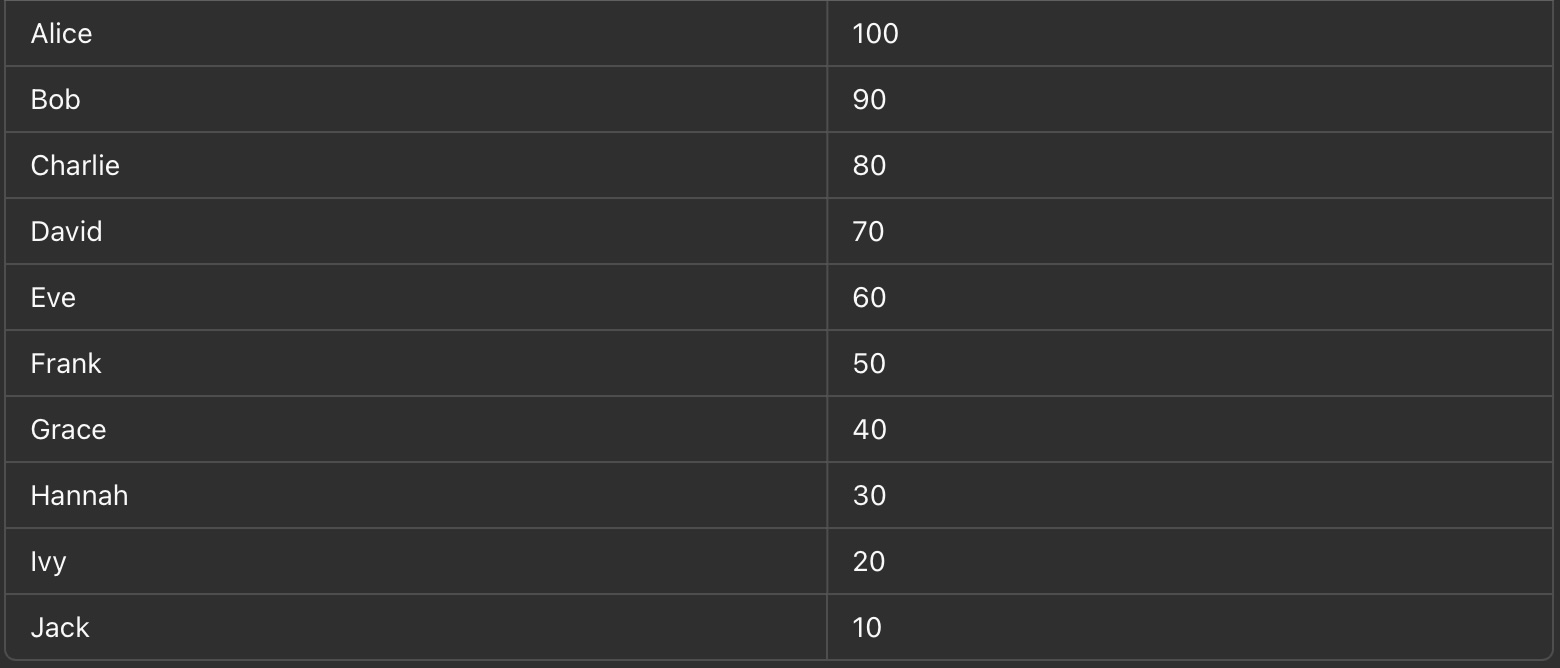
\includegraphics[width=0.9\textwidth,height=\textheight]{./images/Vector-2.jpg}

This example is a 2-dimensional data frame that holds 10 rows and 2
columns. This is an example of a \textbf{data frame}. In a data frame,
each row is called an \textbf{observation} and each column is called a
\textbf{variable}. This data frame has two variables: \texttt{name} and
\texttt{test\_score}. The \texttt{name} variable holds the names of the
students in the class, while the \texttt{test\_score} variable holds the
test scores of the students.

When creating a new data frame, you want to make sure you are giving it
a name that makes sense. For example, if you are creating a data frame
that holds the names of the students in a class along with their test
scores, you might want to name it \texttt{student\_data}. This will help
you remember what the data frame is for when you are working with it
later.

In order to create a data frame, we can use the \texttt{data.frame()}
function. This function is used to create a new data frame. For example,
if we wanted to create a data frame that holds the names of the students
in a class along with their test scores, we could do it like this:

\begin{Shaded}
\begin{Highlighting}[]
\NormalTok{student\_data }\OtherTok{\textless{}{-}} \FunctionTok{data.frame}\NormalTok{(}
  \AttributeTok{name =} \FunctionTok{c}\NormalTok{(}\StringTok{"Alice"}\NormalTok{, }\StringTok{"Bob"}\NormalTok{, }\StringTok{"Charlie"}\NormalTok{, }\StringTok{"David"}\NormalTok{, }\StringTok{"Eve"}\NormalTok{, }\StringTok{"Frank"}\NormalTok{, }\StringTok{"Grace"}\NormalTok{, }\StringTok{"Hannah"}\NormalTok{, }\StringTok{"Ivy"}\NormalTok{, }\StringTok{"Jack"}\NormalTok{),}
  \AttributeTok{test\_score =} \FunctionTok{c}\NormalTok{(}\DecValTok{100}\NormalTok{, }\DecValTok{90}\NormalTok{, }\DecValTok{80}\NormalTok{, }\DecValTok{70}\NormalTok{, }\DecValTok{60}\NormalTok{, }\DecValTok{50}\NormalTok{, }\DecValTok{40}\NormalTok{, }\DecValTok{30}\NormalTok{, }\DecValTok{20}\NormalTok{, }\DecValTok{10}\NormalTok{)}
\NormalTok{)}

\FunctionTok{class}\NormalTok{(student\_data)}
\end{Highlighting}
\end{Shaded}

\begin{verbatim}
[1] "data.frame"
\end{verbatim}

In this example, we are creating a data one column at a time. Since we
named these columns as \texttt{name} and \texttt{test\_score}, we can
access the values in the same way as we would with a vector. For
example, if we wanted to access the first value in the \texttt{name}
column, we could do it like this: \texttt{student\_data\$name{[}1{]}}.
This would return the value \texttt{Alice}.

\begin{Shaded}
\begin{Highlighting}[]
\NormalTok{student\_data}\SpecialCharTok{$}\NormalTok{name[}\DecValTok{1}\NormalTok{]}
\end{Highlighting}
\end{Shaded}

\begin{verbatim}
[1] "Alice"
\end{verbatim}

Similarly, if we wanted to access the first value in the
\texttt{test\_score} column, we could do it like this:
\texttt{student\_data\$test\_score{[}1{]}}. This would return the value
\texttt{100}.

\begin{Shaded}
\begin{Highlighting}[]
\NormalTok{student\_data}\SpecialCharTok{$}\NormalTok{test\_score[}\DecValTok{1}\NormalTok{]}
\end{Highlighting}
\end{Shaded}

\begin{verbatim}
[1] 100
\end{verbatim}

We could also the value in the fifth row and second column like this:

\begin{Shaded}
\begin{Highlighting}[]
\NormalTok{student\_data[}\DecValTok{5}\NormalTok{, }\DecValTok{2}\NormalTok{]}
\end{Highlighting}
\end{Shaded}

\begin{verbatim}
[1] 60
\end{verbatim}

If we wanted to print out the entire first column, we could do it like
this:

\begin{Shaded}
\begin{Highlighting}[]
\NormalTok{student\_data}\SpecialCharTok{$}\NormalTok{name}
\end{Highlighting}
\end{Shaded}

\begin{verbatim}
 [1] "Alice"   "Bob"     "Charlie" "David"   "Eve"     "Frank"   "Grace"  
 [8] "Hannah"  "Ivy"     "Jack"   
\end{verbatim}

If we wanted to print out the entire second column, we could do it like
this:

\begin{Shaded}
\begin{Highlighting}[]
\NormalTok{student\_data}\SpecialCharTok{$}\NormalTok{test\_score}
\end{Highlighting}
\end{Shaded}

\begin{verbatim}
 [1] 100  90  80  70  60  50  40  30  20  10
\end{verbatim}

What happens if we wanted to print out the entore data frame? We could
do it like this:

\begin{Shaded}
\begin{Highlighting}[]
\NormalTok{student\_data}
\end{Highlighting}
\end{Shaded}

\begin{verbatim}
      name test_score
1    Alice        100
2      Bob         90
3  Charlie         80
4    David         70
5      Eve         60
6    Frank         50
7    Grace         40
8   Hannah         30
9      Ivy         20
10    Jack         10
\end{verbatim}

These commands are nice, but if you have a large data set then just
printing it off can be a bit overwhelming. We can use the
\texttt{head()} function to print out the first few rows of the data
frame. For example, if we wanted to print out the first 3 rows of the
data frame, we could do it like this:

\begin{Shaded}
\begin{Highlighting}[]
\FunctionTok{head}\NormalTok{(student\_data, }\DecValTok{3}\NormalTok{)}
\end{Highlighting}
\end{Shaded}

\begin{verbatim}
     name test_score
1   Alice        100
2     Bob         90
3 Charlie         80
\end{verbatim}

If we wanted to print out the last few rows of the data frame, we could
use the \texttt{tail()} function. For example, if we wanted to print out
the last 5 rows

\begin{Shaded}
\begin{Highlighting}[]
\FunctionTok{tail}\NormalTok{(student\_data, }\DecValTok{5}\NormalTok{)}
\end{Highlighting}
\end{Shaded}

\begin{verbatim}
     name test_score
6   Frank         50
7   Grace         40
8  Hannah         30
9     Ivy         20
10   Jack         10
\end{verbatim}

The default amount of lines for \texttt{head()} and \texttt{tail()} is
6. If you don't specify an amount of lines, it will print out 6 lines.

\begin{Shaded}
\begin{Highlighting}[]
\FunctionTok{head}\NormalTok{(student\_data)}
\end{Highlighting}
\end{Shaded}

\begin{verbatim}
     name test_score
1   Alice        100
2     Bob         90
3 Charlie         80
4   David         70
5     Eve         60
6   Frank         50
\end{verbatim}

How is a data frame different from a tibble? Let's talk about that next.

\section*{Tibbles}\label{tibbles}
\addcontentsline{toc}{section}{Tibbles}

\markright{Tibbles}

A tibble is a modern version of a data frame that is part of the
\textbf{tidyverse}. It is similar to a data frame, but it has some
additional features that make it easier to work with. For example,
tibbles have a nicer print method that makes it easier to view the data.
They also have some additional functions that make it easier to
manipulate the data. For example, you can use the \texttt{select()}
function to select specific columns from a tibble. You can also use the
\texttt{filter()} function to filter rows based on a condition. These
functions make it easier to work with tibbles than with data frames.

In order to create a tibble, we can use the \texttt{tibble()} function.
This function is used to create a new tibble. For example, if we wanted
to create a tibble that holds the names of the students in a class along
with their test scores, we could do it like this:

\begin{Shaded}
\begin{Highlighting}[]
\CommentTok{\# Make sure tidyverse is installed and loaded up. Remember, if you}
\CommentTok{\# need to install it, use the following :}

\CommentTok{\# install.packages(tidyverse)}
\end{Highlighting}
\end{Shaded}

\begin{Shaded}
\begin{Highlighting}[]
\CommentTok{\# If it is already downloaded, then you just need to load up the library :}

\FunctionTok{library}\NormalTok{(tidyverse)}
\end{Highlighting}
\end{Shaded}

\begin{verbatim}
-- Attaching core tidyverse packages ------------------------ tidyverse 2.0.0 --
v dplyr     1.1.4     v readr     2.1.5
v forcats   1.0.0     v stringr   1.5.1
v ggplot2   3.5.1     v tibble    3.2.1
v lubridate 1.9.4     v tidyr     1.3.1
v purrr     1.0.2     
-- Conflicts ------------------------------------------ tidyverse_conflicts() --
x dplyr::filter() masks stats::filter()
x dplyr::lag()    masks stats::lag()
i Use the conflicted package (<http://conflicted.r-lib.org/>) to force all conflicts to become errors
\end{verbatim}

\begin{Shaded}
\begin{Highlighting}[]
\CommentTok{\# I have already installed the tibble package, so I will just load it up}

\FunctionTok{library}\NormalTok{(tibble)}

\NormalTok{student\_data2 }\OtherTok{\textless{}{-}} \FunctionTok{tibble}\NormalTok{(}
  \AttributeTok{name =} \FunctionTok{c}\NormalTok{(}\StringTok{"Alice"}\NormalTok{, }\StringTok{"Bob"}\NormalTok{, }\StringTok{"Charlie"}\NormalTok{, }\StringTok{"David"}\NormalTok{, }\StringTok{"Eve"}\NormalTok{, }\StringTok{"Frank"}\NormalTok{, }\StringTok{"Grace"}\NormalTok{, }\StringTok{"Hannah"}\NormalTok{, }\StringTok{"Ivy"}\NormalTok{, }\StringTok{"Jack"}\NormalTok{),}
  \AttributeTok{test\_score =} \FunctionTok{c}\NormalTok{(}\DecValTok{100}\NormalTok{, }\DecValTok{90}\NormalTok{, }\DecValTok{80}\NormalTok{, }\DecValTok{70}\NormalTok{, }\DecValTok{60}\NormalTok{, }\DecValTok{50}\NormalTok{, }\DecValTok{40}\NormalTok{, }\DecValTok{30}\NormalTok{, }\DecValTok{20}\NormalTok{, }\DecValTok{10}\NormalTok{)}
\NormalTok{)}

\FunctionTok{class}\NormalTok{(student\_data2)}
\end{Highlighting}
\end{Shaded}

\begin{verbatim}
[1] "tbl_df"     "tbl"        "data.frame"
\end{verbatim}

In this example, we are creating a tibble that is similar to the data
frame we created earlier. The main difference is that this tibble is
part of the tidyverse. This means that it has some additional features
that make it easier to work with. For example, we can use the
\texttt{select()} function to select specific columns from the tibble.
For example, if we wanted to select the \texttt{name} column from the
tibble, we could do it like this:

\begin{Shaded}
\begin{Highlighting}[]
\FunctionTok{select}\NormalTok{(student\_data2, name)}
\end{Highlighting}
\end{Shaded}

\begin{verbatim}
# A tibble: 10 x 1
   name   
   <chr>  
 1 Alice  
 2 Bob    
 3 Charlie
 4 David  
 5 Eve    
 6 Frank  
 7 Grace  
 8 Hannah 
 9 Ivy    
10 Jack   
\end{verbatim}

If we wanted to select the \texttt{test\_score} column from the tibble,
we could do it like this:

\begin{Shaded}
\begin{Highlighting}[]
\FunctionTok{select}\NormalTok{(student\_data2, test\_score)}
\end{Highlighting}
\end{Shaded}

\begin{verbatim}
# A tibble: 10 x 1
   test_score
        <dbl>
 1        100
 2         90
 3         80
 4         70
 5         60
 6         50
 7         40
 8         30
 9         20
10         10
\end{verbatim}

If I want all of the students that got higher than a 65 for their test
score, I could use the \texttt{filter()} command to help us out. The
\texttt{filter()} command needs two arguments. The first is the name of
the tibble and the second is the condition that we want to filter on.
For example, if we wanted to filter out all of the students that got
higher than a 65 on their test, we could do it like this:

\begin{Shaded}
\begin{Highlighting}[]
\FunctionTok{filter}\NormalTok{(student\_data2, test\_score }\SpecialCharTok{\textgreater{}} \DecValTok{65}\NormalTok{)}
\end{Highlighting}
\end{Shaded}

\begin{verbatim}
# A tibble: 4 x 2
  name    test_score
  <chr>        <dbl>
1 Alice          100
2 Bob             90
3 Charlie         80
4 David           70
\end{verbatim}

Another advantage a tibble has over a data frame is that it is easier to
work with when you are working with large data sets. For example, if you
have a data set that has 1 million rows, it can be difficult to work
with a data frame. This is because data frames are stored in memory, and
if you have a large data set, it can take up a lot of memory. This can
slow down your computer and make it difficult to work with the data.
Tibbles are designed to be more memory efficient than data frames. This
means that they can handle larger data sets more easily. This makes it
easier to work with large data sets in R.

In conclusion, vectors, data frames, and tibbles are all useful
structures that can be used to store data. Vectors are 1-dimensional
structures that can hold multiple elements. Data frames are
2-dimensional structures that can hold multiple elements. Tibbles are a
modern version of data frames that are part of the tidyverse. They have
some additional features that make them easier to work with. All of
these structures are useful for storing data in R, and you will likely
use all of them at some point when working with data in R.

\bookmarksetup{startatroot}

\chapter*{Statistics Language}\label{statistics-language}
\addcontentsline{toc}{chapter}{Statistics Language}

\markboth{Statistics Language}{Statistics Language}

As we start to consider analyzing data, we need to be able to
communicate with other data scientists. This is where statistics
language comes in. We want to take some time to define some terms that
we will be using throughout the course. For now we will just focus on
foundational terms. As we develop different analytic skills, we will
introduce more terms.

\subsection*{Population}\label{population}
\addcontentsline{toc}{subsection}{Population}

The population is the entire group that we are interested in studying.
For example, if we are interested in studying the average height of all
people in the United States, then the population would be all people in
the United States.

\subsection*{Parameter}\label{parameter}
\addcontentsline{toc}{subsection}{Parameter}

A parameter is a number that describes a population. For example, the
average height of all people in the United States is a parameter. Two of
the more common parameters are the mean and the standard deviation.
These are used to describe the central tendency and the spread of a
population. The mean is typically denoted by the Greek letter mu (μ) and
the standard deviation is typically denoted by the Greek letter sigma
(σ). We will briefly talk about these measures below and go into more
detail in later sections.

Many studies that are done are ones that are trying to estimate a
parameter. Unfortunately, there is only one way to know the true value
of a parameter and that is to measure the entire population. This is not
feasible in most cases as the amount of time and resources to contact
every member of a population is not practical. We can, however, take
what is called a sample of the population and use that to estimate the
parameter.

\subsection*{Sample}\label{sample}
\addcontentsline{toc}{subsection}{Sample}

A sample is a subset of the population. For example, if we are
interested in studying the average height of all people in the United
States, then a sample could be a group of 100 people from the United
States. This is a much easier way to get information about the
population rather than having to contact every member of the population.

There are several different methods one can use to take a sample. We
will discuss these methods in later sections.

\subsection*{Statistic}\label{statistic}
\addcontentsline{toc}{subsection}{Statistic}

A statistic is a number that describes a sample. For example, the
average height of a group of 100 people from the United States is a
statistic. Two of the more common statistics are the sample mean and the
sample standard deviation. These are used to describe the central
tendency and the spread of a sample. The sample mean is typically
denoted by the letter x-bar (x̄) and the sample standard deviation is
typically denoted by the letter s.

If we are trying to answer a question about the population, for instance
the average height of all people in the United States, we can take a
sample of the population and use the value from the sample as an
estimate for the parameter from the population. This is the basis of
inferential statistics, which we mention next.

\subsection*{Inferential Statistics}\label{inferential-statistics}
\addcontentsline{toc}{subsection}{Inferential Statistics}

Inferential statistics are used to make inferences from a sample to a
population. In other words, inferential statistics are used to make
predictions about a population based on a sample. The following graphic
demonstrates the process.

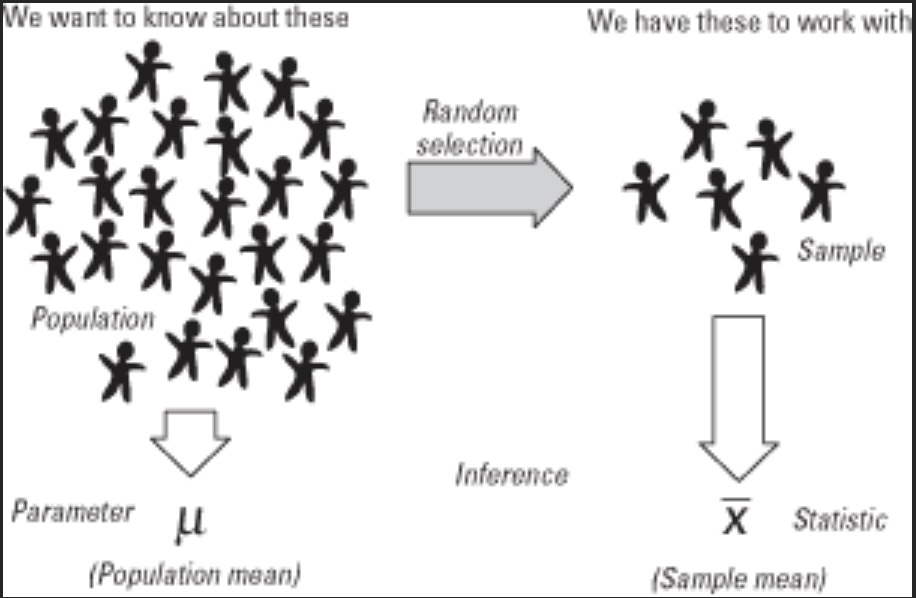
\includegraphics[width=0.4\textwidth,height=\textheight]{./images/SL_1.jpg}

\begin{itemize}
\tightlist
\item
  We are wanting to determine a population parameter μ
\item
  We take a sample from the population
\item
  Calculate the value of the statistic x̄ from the sample.
\item
  Use the sample statistic x to estimate the population parameter μ.
\end{itemize}

This process is the basis of inferential statistics. Using the sample to
help us determine estimates of the population parameter.

\subsection*{Descriptive Statistics}\label{descriptive-statistics}
\addcontentsline{toc}{subsection}{Descriptive Statistics}

Descriptive statistics are used to describe the basic features of the
data in a study. They provide simple summaries about the sample and the
measures. For our purposes we will focus on measures of central tendency
(mean, median, mode) and measures of spread (standard deviation,
variance, 5-Number summary). We will discuss these in more detail in
later sections.

\subsection*{Confidence Interval}\label{confidence-interval}
\addcontentsline{toc}{subsection}{Confidence Interval}

We are using a sample to estimate a population parameter. Unfortunately,
if we were to take multiple samples from the population, we would get
different values for the parameter. This is because the sample is only a
portion of the population. The sample you take the first time is almost
assuredly going to be different from the sample you take the second
time. This means that the statistic from the first sample is going to be
different from the statistic from the second sample.

This is the reason why we will estimate a parameter with a confidence
interval. A confidence interval is a range of values that is likely to
contain the true value of a parameter. For example, a 95\% confidence
interval for the average height of all people in the United States would
be a range of values that is likely to contain the true average height
with 95\% confidence. The confidence interval is based on the sample
statistic and a margin of error. The higher the confidence level, the
wider the confidence interval. We will discuss confidence intervals in
more detail in later sections.

\subsection*{Distribution}\label{distribution}
\addcontentsline{toc}{subsection}{Distribution}

The distribution of a data set tells us two things : the values in the
data set and how often they occur.

Here is an example of a distribution of the number of times a person
goes to the gym in a week.

\begin{Shaded}
\begin{Highlighting}[]
\CommentTok{\# We need the tibble function, so load up the tidyverse package}

\FunctionTok{library}\NormalTok{(tidyverse)}
\end{Highlighting}
\end{Shaded}

\begin{Shaded}
\begin{Highlighting}[]
\CommentTok{\# Create a data frame}

\NormalTok{df }\OtherTok{\textless{}{-}} \FunctionTok{tibble}\NormalTok{(}
  \AttributeTok{gym\_visits =} \FunctionTok{c}\NormalTok{(}\DecValTok{0}\NormalTok{, }\DecValTok{1}\NormalTok{, }\DecValTok{2}\NormalTok{, }\DecValTok{3}\NormalTok{, }\DecValTok{4}\NormalTok{, }\DecValTok{5}\NormalTok{, }\DecValTok{6}\NormalTok{, }\DecValTok{7}\NormalTok{),}
  \AttributeTok{frequency =} \FunctionTok{c}\NormalTok{(}\DecValTok{10}\NormalTok{, }\DecValTok{20}\NormalTok{, }\DecValTok{30}\NormalTok{, }\DecValTok{40}\NormalTok{, }\DecValTok{50}\NormalTok{, }\DecValTok{40}\NormalTok{, }\DecValTok{30}\NormalTok{, }\DecValTok{20}\NormalTok{)}
\NormalTok{)}

\NormalTok{df}
\end{Highlighting}
\end{Shaded}

\begin{verbatim}
# A tibble: 8 x 2
  gym_visits frequency
       <dbl>     <dbl>
1          0        10
2          1        20
3          2        30
4          3        40
5          4        50
6          5        40
7          6        30
8          7        20
\end{verbatim}

In this example, the distribution tells us how many times a person goes
to the gym in a week and how often that occurs. For example, 40 people
go to the gym 3 times a week or 30 people go to the gym 6 times a week.

\subsection*{Outlier}\label{outlier}
\addcontentsline{toc}{subsection}{Outlier}

An outlier is a data point that is significantly different from the
other data points in a dataset. Outliers can have a significant impact
on the results of statistical analyses, especially for means and
standard deviations. Outliers can be caused by errors in data
collection, measurement error, or natural variation in the data.

In the following example, if someone went to the gym 15 times in a week
would be considered an outlier. This is because the number of times a
person goes to the gym in a week is typically between 0 and 7.

Depending on the data set, outliers could occur in either the high or
the low direction.

\subsection*{Normal Distribution}\label{normal-distribution}
\addcontentsline{toc}{subsection}{Normal Distribution}

One of the more typical distributions one will work with is the normal
distribution. A normal distribution is a symmetric unimodal
distributionin which the values are distributed around the mean
according to a bell-shaped curve. The normal distribution is
characterized by its mean and standard deviation. In other words, the
mean and standard deviation determine the shape of the normal
distribution. The mean determines the center of the distribution and the
standard deviation determines the height and width of the distribution.

\subsection*{Skewness}\label{skewness}
\addcontentsline{toc}{subsection}{Skewness}

Once we know the distribution of a data set, we will often draw a
picture of the distribution. One of the descriptors we will look for is
skewness. Skewness is a measure of the asymmetry of a distribution. A
distribution is symmetric if the left and right sides are mirror images
of each other. A distribution is positively skewed (or skewed to the
right)\\
if the right tail is longer than the left tail, and negatively skewed
(or skewed left) if the left tail is longer than the right tail.

Here is a graphic giving examples of each type of skewness.

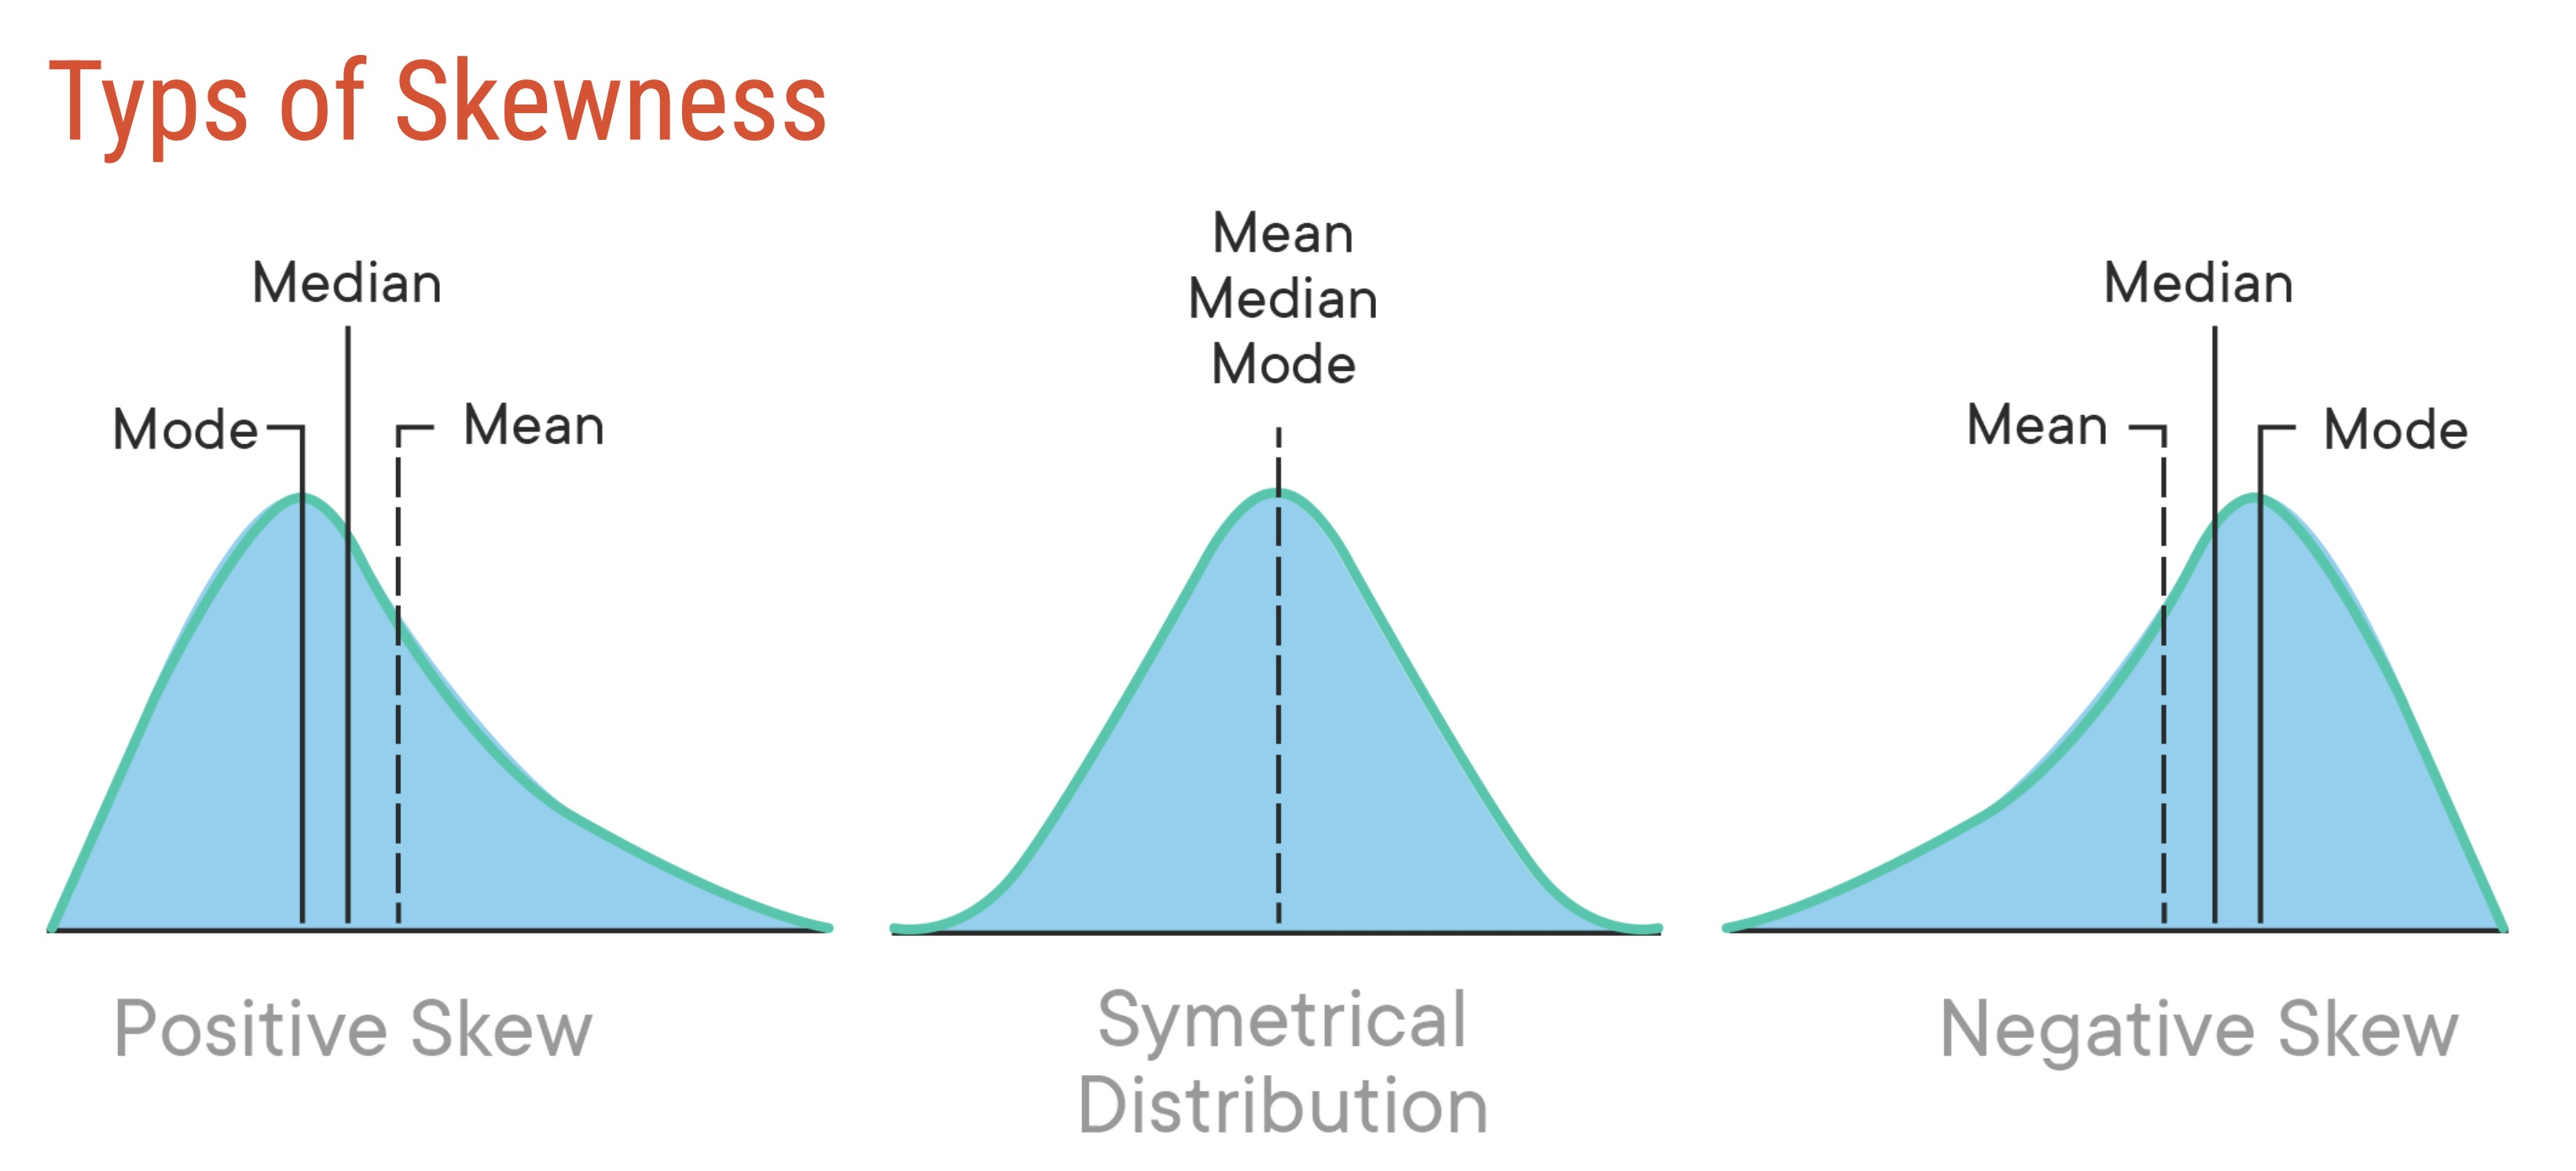
\includegraphics[width=0.6\textwidth,height=\textheight]{./images/SL_2.jpg}

\bookmarksetup{startatroot}

\chapter*{Measures Of Central
Tendencies}\label{measures-of-central-tendencies}
\addcontentsline{toc}{chapter}{Measures Of Central Tendencies}

\markboth{Measures Of Central Tendencies}{Measures Of Central
Tendencies}

Note : Many of the graphics and descriptions may be found here :
https://www.r4epi.com/measures-of-central-tendency

We have gotten to the point where we are starting to describe a given
data set. Here is where we are, as of now :

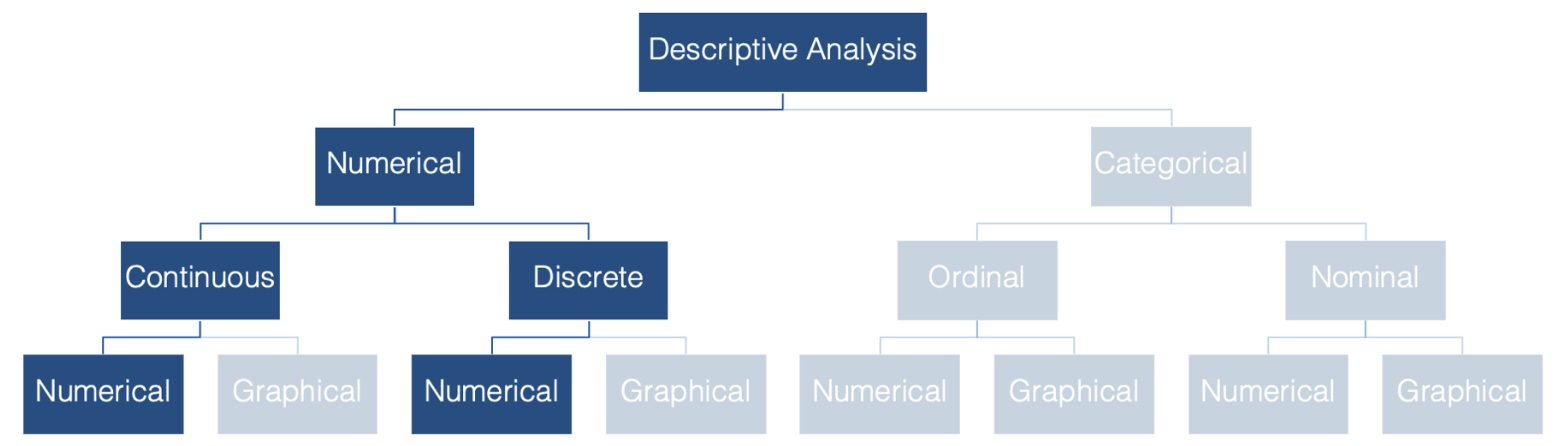
\includegraphics[width=0.75\textwidth,height=\textheight]{./images/Daily-4-Pic-1.jpg}

Why do we want to be able to describe the central tendency of a data
set? Consider epidemiology. In epidemiology, we often want to describe
the ``typical'' person in a population with respect to some
characteristic that is recorded as a numerical variable -- like height
or weight. The most basic, and probably most commonly used, way to do so
is with a measure of central tendency.

In this lesson we have discussed three measures of central tendency:

\begin{itemize}
\tightlist
\item
  The mean
\item
  The median
\item
  The mode
\end{itemize}

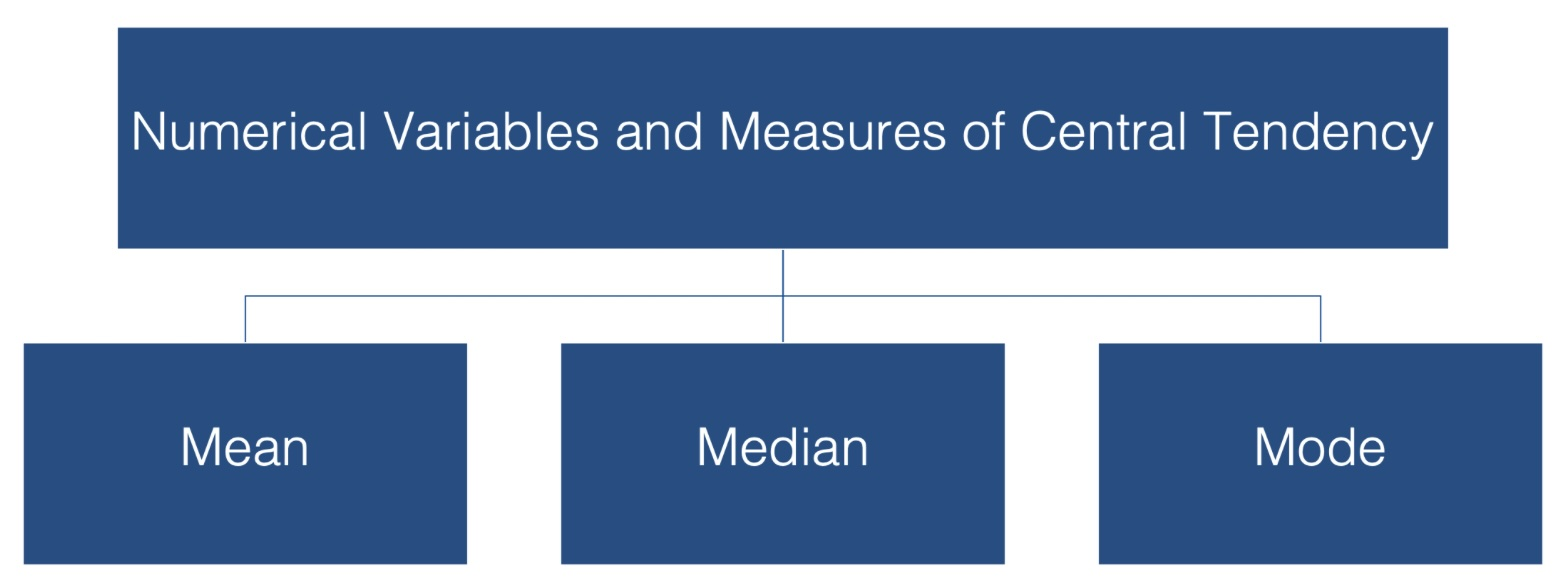
\includegraphics[width=0.5\textwidth,height=\textheight]{./images/Daily-4-Pic-2.jpg}

\subsection*{The Mean}\label{the-mean}
\addcontentsline{toc}{subsection}{The Mean}

When we talk about the typical, or ``average'', value of some variable
measured on a continuous scale, we are usually talking about the mean
value of that variable. To be even more specific, we are usually talking
about the arithmetic mean value. This value has some favorable
characteristics that make it a good description of central tendency.

\begin{itemize}
\item
  For starters it's simple. Most people are familiar with the mean, and
  at the very least, have some intuitive sense of what it means (no pun
  intended).
\item
  In addition, there can be only one mean value for any set of values.
\end{itemize}

However, there are a couple of potentially problematic characteristics
of the mean as well:

\begin{itemize}
\item
  It's susceptible to extreme values in your data. In other words, a
  couple of people with very atypical values for the characteristic you
  are interested in can drastically alter the value of the mean, and
  your estimate for the typical person in your population of interest
  along with it.
\item
  Additionally, it's highly likely to calculate a mean value that is not
  actually observed anywhere in your data.
\end{itemize}

Let's assume we have a data set with \(n\) points and we label them as
\(a_1\), \(a_2\), . . . \(a_n\). Here is the fancy, schmancy formula for
finding the Average / Mean :

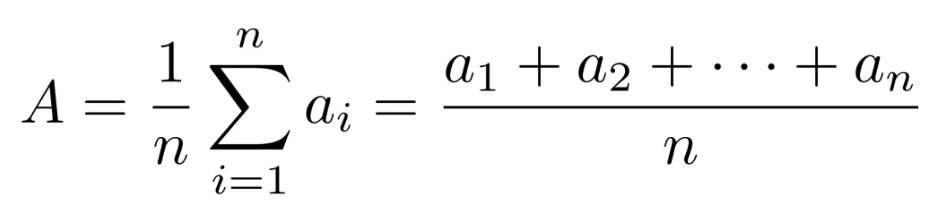
\includegraphics[width=0.4\textwidth,height=\textheight]{./images/Daily-4-Pic-8.jpg}

The capital sigma there is a mathematical symbol that tells us to sum up
what ever follows the sigma and we will then divide by \(n\) which is
the number of points we have in the data set. It can be said a little
easier as :

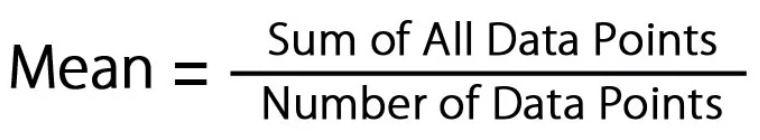
\includegraphics[width=0.35\textwidth,height=\textheight]{./images/Daily-4-Pic-9.jpg}

\textbf{Caution :} The mean is a nice way to get a value that describes
the centrality of a data set, but it can sometimes be problematic if
there are values that drastically higher or lower than most of the
values in a data set.

Consider this data set :

\(1 \,\,\,2 \,\,\,3\,\,\,4\,\,\,5\,\,\,6\,\,\,7\,\,\,8\,\,\,9\)

We can quickly calculate the average to be
\[(1 + 2 + 3 + \dots +9\,)\,/\,9 = \frac{45}{9}=5\] which is right smack
dab in the middle of the data set. 50\% of the scores are above and
below the value for the average, os it is a very good measure of
centrality for this set.

However, adding a single value can sometimes make the average a poor
choice for measure of centrality. Consider adding the value \(100\) to
the previous data set :

\(1 \,\,\,2 \,\,\,3\,\,\,4\,\,\,5\,\,\,6\,\,\,7\,\,\,8\,\,\,9\,\,\,100\)

Calculating the average for this data set yields as average of :
\[(1 + 2 + 3 + \dots +9+100\,)\,/\,9 = \frac{145}{10} = 14.5\] In this
example, the mean is actually larger than 90\% of all the scores in the
data set. That means it is a \textbf{poor} choice as a representative
value for the data set.

Note that scores that are far away from most of the values in a data set
are called \textbf{outliers} and as you will see, even a single outlier
can vastly affect the mean. This means that the mean is \textbf{not}
resistant to outliers!

This is one of the reasons why it is important that there is more than
one option as a measure of centrality.

\subsection*{The Median}\label{the-median}
\addcontentsline{toc}{subsection}{The Median}

The median is probably the second most commonly used measure of central
tendency.

\begin{itemize}
\item
  Like the mean, it's computationally simple and relatively
  straightforward to understand.
\item
  There can be one, and only one, median.
\item
  And, its value may also be unobserved in the data.
\end{itemize}

The idea of finding the Median is fairly simple :

\begin{itemize}
\item
  Line up the values from smallest to largest
\item
  The value that occurs in the middle will be the \textbf{median}
\item
  This means the \textbf{median} scores has half of the values
  \textbf{below it} and half the values \textbf{above it}, when you
  exclude the spot representing the median.
\end{itemize}

There is a small caveat depending on if there is an even or odd amount
of values in the data set. Let's assume there are \textbf{n} values in
the data set.

Let's assume \textbf{n is odd}. Consider this example where we have a
data set with 7 values, where the data has already been arranged from
smallest to largest:

\includegraphics[width=0.3\textwidth,height=\textheight]{./images/Daily-4-Pic-4.jpg}

When \textbf{n is odd}, the median is the value located in spot
\textbf{(n+1)/2}. So in this case the median is located in spot
\((7+1)/2 = 4\)th spot :

\includegraphics[width=0.3\textwidth,height=\textheight]{./images/Daily-4-Pic-5.jpg}

Notice that when we exclude the median, we have just as many values
\textbf{below} the median (3) as we have \textbf{above} the median (3).

\textbf{Important :} The \textbf{median} is a \textbf{spot-based}
measure. We are looking for the value that occurs in the middle spot. In
this example, the median was in spot 4 with the median taking on the
value of 18.

It is entirely possible that the median takes on a value below or above
this spot if there are repeated values. Consider a similar data set :

\(8\,\,\, 11\,\,\,  15\,\,\,  15\,\,\,  24\,\,\,  30\,\,\,  31\)

In this example, there are still 7 values in the data set so the median
is still located in spot 4 :

\(8\,\,\, 11\,\,\,  15\,\,\,  \underline{\,\,15\,\,}\,\,\,  24\,\,\,  30\,\,\,  31\)

In this case, the median takes on the value in the fourth spot, namely
15. We still have three values below the median :
\(8\,\,\, 11 \,\,\, 15\,\) and three values above the median :
\(24 \,\,\, 30\,\,\, 31\,\). So even though we have a value for the
median that is also in a different spot of the data set, we still have
50\% of the scores above the median and 50\% of the scores below the
median. This means that the important aspect of finding the median is
finding the \textbf{spot} that is in the middle and that will inform us
on the value of the median.

What happens when \textbf{n is even}? This complicates the process a bit
because there is not a single value that falls in the middle. Consider
this example of an already ordered set of six values :

\includegraphics[width=0.3\textwidth,height=\textheight]{./images/Daily-4-Pic-6.jpg}

As you can see above, we don't have a single spot that is right in the
middle that we can call the median. However, we do have \textbf{two}
values in the middle. In this case, those values are \textbf{18} and
\textbf{24}. To get the median, we will simply find the average of these
two values to create the median.

Finding the two middle spots is simple. The first value is located in
spot \((n\,/\,2)\) and the second spot in lcoated immediatley following,
\((n\,/\,2) + 1\). In the following example we have a data set with
\(6\) values. Since this is an even amount of values, we will work with
the values in spots \((6\,/\,2\,) = 3\) and \((6\,/\,2\,) + 1 = 4\)

\includegraphics[width=0.3\textwidth,height=\textheight]{./images/Daily-4-Pic-7.jpg}

As you can see spot 3 has the value \(18\) and spot 4 has the value
\(24\). The median is the average of these two values. Therefore the
median is \((18 + 24)/2 = (42) / 2 = 21\).

Note that in this case we still have the same amount of scores
\textbf{below} the median as we have \textbf{above} the median. This
shows us that 50\% of the data set is below this value and 50\% above
this value which is the definition of median.

An interesting result is that in this case the median is \textbf{not} a
value from the data set! If you look at the orginal six values in the
data set, 21 is not one of them! If you have a data set with an even
amount of values, this will almost always be the case. THe only time
where the median will actually be a value on in the data set is if the
two values in the middle happen to be the exact same value. Otherwise,
the median will be a value not in the original data set.

Let's revisit an issue we discovered when discussing averages, namely
outliers. How do outliers affect the median?

Let calculate the median for the following two data sets :

\(1 \,\,\,2 \,\,\,3\,\,\,4\,\,\,5\,\,\,6\,\,\,7\,\,\,8\,\,\,9\)

In this example, there are \(9\) scores, which tells us the median is
located in spot \(\frac{9+1}{2} = \frac{10}{2}= 5\). Spot 5 happens to
contain the value \(5\). Notice that this stil has 50\% of the scores
below and 50\% of the scores above the median which tells us it is a
good representative for the measure of centrality.

What does adding an outlier do? How does it affect the median? Let's
explore and find out.

\(1 \,\,\,2 \,\,\,3\,\,\,4\,\,\,5\,\,\,6\,\,\,7\,\,\,8\,\,\,9\,\,\,100\)

We now have 10 scores which means we want to take the average of the tow
middle scores in spots \(\frac{10}{2} = 5\) and
\(\frac{10}{2} + 1 = 6\).

\(1 \,\,\,2 \,\,\,3\,\,\,4\,\,\underline{\,5\,}\,\,\,\underline{\,6\,}\,\,7\,\,\,8\,\,\,9\,\,\,100\)

The average of these two values gives us \(\frac{5 + 6}{2} = 5.5\).
Again, think about the definition of a measure of centrality. If you
consider the median to be 5.5, then notice there are 5 values below the
median and 5 valuse above the median, showing us that this is a good
representative for the measure of centrality.

This tells us that outliers do not affect the median very much at all.
The median moved from \(5\) up to \(5.5\). What this shows us is that
medians \textbf{are resistant} to outiers!

\begin{tcolorbox}[enhanced jigsaw, colbacktitle=quarto-callout-important-color!10!white, colframe=quarto-callout-important-color-frame, opacitybacktitle=0.6, rightrule=.15mm, title=\textcolor{quarto-callout-important-color}{\faExclamation}\hspace{0.5em}{Important}, colback=white, coltitle=black, breakable, leftrule=.75mm, toptitle=1mm, bottomrule=.15mm, opacityback=0, bottomtitle=1mm, titlerule=0mm, left=2mm, toprule=.15mm, arc=.35mm]

This means that if we have a data set that contains outliers, we need to
consider using the median as the measure of centrality and not the mean.
This raises the question of when does a data set have outliers, and this
will be discussed when we talk about Measures of Spread.

\end{tcolorbox}

\subsection*{The Mode}\label{the-mode}
\addcontentsline{toc}{subsection}{The Mode}

And finally, we have the mode, or the value that is most often observed
in the data. It doesn't get much simpler than that. But, unlike the mean
and the median, there can be more than one mode for a given set of
values. In fact, there can even be no mode if all the values are
observed the exact same number of times. However, if there is a mode, by
definition it's observed in the data.

Consider these examples :

\textbf{Mode Example 1}

\(8\,\,\, 11\,\,\,  15\,\,\,  15\,\,\,  24\,\,\,  30\,\,\,  31\)

In this data set, then value \(15\) appears twice and everything else
appears once. Therefore the mode of this data set is \(15\).

\textbf{Mode Example 2}

\(8\,\,\, 11\,\,\,  15\,\,\,  15\,\,\,  24\,\,\,  30\,\,\,  30\,\,\ 31\)

In this data set, then value \(15\) \textbf{and} \(30\) appear twice and
everything else appears once. Therefore the mode of this data set is
\(15\) \textbf{and} \(30\).

\textbf{Mode Example 3}

\(8\,\,\, 11\,\,\,  12\,\,\,  15\,\,\,  24\,\,\,  30\,\,\,  33\,\,\ 37\)

In this data set, \textbf{no} value appears more than any other value,
so this data set \textbf{does not} have a mode!

\subsection*{Summary}\label{summary-1}
\addcontentsline{toc}{subsection}{Summary}

Here is a graphic that reviews what we have discussed so far :

\includegraphics[width=0.6\textwidth,height=\textheight]{./images/Daily-4-Pic-10.jpg}

\subsection*{Calculating the Mean and
Median}\label{calculating-the-mean-and-median}
\addcontentsline{toc}{subsection}{Calculating the Mean and Median}

Now that we are all on the same page with respect to the fundamentals of
central tendency, let's remind ourselves how to calculate these measures
using R.

Calculating the mean is really straightforward. We can just use base R's
built-in \textbf{mean( )} function.

Load the \textbf{dplyr} package. We will need several \textbf{dplyr}
functions and can install and load the package with the code below.

\begin{Shaded}
\begin{Highlighting}[]
\CommentTok{\# Here is the command of we need to install the package. }

\CommentTok{\# install.packages("dplyr")}

\CommentTok{\# We can load the dplyr pack :}

\FunctionTok{library}\NormalTok{(dplyr)}
\end{Highlighting}
\end{Shaded}

We can simulate some data by typing (cut and paste?) the following into
your code:

\begin{Shaded}
\begin{Highlighting}[]
\CommentTok{\# Load up tibble, if needed}

\FunctionTok{library}\NormalTok{(tibble)}

\CommentTok{\# We can now create the tibble}

\NormalTok{height\_and\_weight\_20 }\OtherTok{\textless{}{-}} \FunctionTok{tribble}\NormalTok{(}
  \SpecialCharTok{\textasciitilde{}}\NormalTok{id,   }\SpecialCharTok{\textasciitilde{}}\NormalTok{sex,     }\SpecialCharTok{\textasciitilde{}}\NormalTok{ht\_in, }\SpecialCharTok{\textasciitilde{}}\NormalTok{wt\_lbs,}
  \StringTok{"001"}\NormalTok{, }\StringTok{"Male"}\NormalTok{,   }\DecValTok{71}\NormalTok{,     }\DecValTok{190}\NormalTok{,}
  \StringTok{"002"}\NormalTok{, }\StringTok{"Male"}\NormalTok{,   }\DecValTok{69}\NormalTok{,     }\DecValTok{177}\NormalTok{,}
  \StringTok{"003"}\NormalTok{, }\StringTok{"Female"}\NormalTok{, }\DecValTok{64}\NormalTok{,     }\DecValTok{130}\NormalTok{,}
  \StringTok{"004"}\NormalTok{, }\StringTok{"Female"}\NormalTok{, }\DecValTok{65}\NormalTok{,     }\DecValTok{153}\NormalTok{,}
  \StringTok{"005"}\NormalTok{, }\ConstantTok{NA}\NormalTok{,       }\DecValTok{73}\NormalTok{,     }\DecValTok{173}\NormalTok{,}
  \StringTok{"006"}\NormalTok{, }\StringTok{"Male"}\NormalTok{,   }\DecValTok{69}\NormalTok{,     }\DecValTok{182}\NormalTok{,}
  \StringTok{"007"}\NormalTok{, }\StringTok{"Female"}\NormalTok{, }\DecValTok{68}\NormalTok{,     }\DecValTok{186}\NormalTok{,}
  \StringTok{"008"}\NormalTok{, }\ConstantTok{NA}\NormalTok{,       }\DecValTok{73}\NormalTok{,     }\DecValTok{185}\NormalTok{,}
  \StringTok{"009"}\NormalTok{, }\StringTok{"Female"}\NormalTok{, }\DecValTok{71}\NormalTok{,     }\DecValTok{157}\NormalTok{,}
  \StringTok{"010"}\NormalTok{, }\StringTok{"Male"}\NormalTok{,   }\DecValTok{66}\NormalTok{,     }\DecValTok{155}\NormalTok{,}
  \StringTok{"011"}\NormalTok{, }\StringTok{"Male"}\NormalTok{,   }\DecValTok{71}\NormalTok{,     }\DecValTok{213}\NormalTok{,}
  \StringTok{"012"}\NormalTok{, }\StringTok{"Female"}\NormalTok{, }\DecValTok{69}\NormalTok{,     }\DecValTok{151}\NormalTok{,}
  \StringTok{"013"}\NormalTok{, }\StringTok{"Female"}\NormalTok{, }\DecValTok{66}\NormalTok{,     }\DecValTok{147}\NormalTok{,}
  \StringTok{"014"}\NormalTok{, }\StringTok{"Female"}\NormalTok{, }\DecValTok{68}\NormalTok{,     }\DecValTok{196}\NormalTok{,}
  \StringTok{"015"}\NormalTok{, }\StringTok{"Male"}\NormalTok{,   }\DecValTok{75}\NormalTok{,     }\DecValTok{212}\NormalTok{,}
  \StringTok{"016"}\NormalTok{, }\StringTok{"Female"}\NormalTok{, }\DecValTok{69}\NormalTok{,     }\DecValTok{19000}\NormalTok{,}
  \StringTok{"017"}\NormalTok{, }\StringTok{"Female"}\NormalTok{, }\DecValTok{66}\NormalTok{,     }\DecValTok{194}\NormalTok{,}
  \StringTok{"018"}\NormalTok{, }\StringTok{"Female"}\NormalTok{, }\DecValTok{65}\NormalTok{,     }\DecValTok{176}\NormalTok{,}
  \StringTok{"019"}\NormalTok{, }\StringTok{"Female"}\NormalTok{, }\DecValTok{65}\NormalTok{,     }\DecValTok{176}\NormalTok{,}
  \StringTok{"020"}\NormalTok{, }\StringTok{"Female"}\NormalTok{, }\DecValTok{65}\NormalTok{,     }\DecValTok{102}
\NormalTok{)}
\end{Highlighting}
\end{Shaded}

In the code above, here are what the steps were :

\begin{itemize}
\item
  We loaded the tibble package so that we could use its tribble()
  function.
\item
  We used the \texttt{tribble(\ )} function to simulate some data --
  heights and weights for 20 hypothetical students.

  \begin{itemize}
  \item
    The \texttt{tribble(\ )} function creates something called a tibble.
    A tibble is the tidyverse version of a data frame. In fact, it is a
    data frame, but with some additional functionality. You can use the
    link to read more about it if you'd like.

    \begin{itemize}
    \tightlist
    \item
      More information on tribble( ) vs tibble( ) vs data.frame
    \end{itemize}
  \item
    We used the tribble( ) function instead of the data.frame( )
    function to create our data frame above because we can use the
    tribble( ) function to create our data frames in rows (like you see
    above) instead of columns with the c( ) function.
  \item
    Using the tribble( ) function to create a data frame isn't any
    better or worse than using the data.frame( ) function. I just wanted
    you to be aware that it exists and is sometimes useful.
  \end{itemize}
\end{itemize}

\textbf{MEAN Example :} Find the mean of the heights in the data frame.

\begin{itemize}
\item
  The name of the tibble is \textbf{height\_and\_weight\_20}.
\item
  The name of the variable we want to use is the column \textbf{ht\_in}
\item
  The way we can access a variable (column) of a data fram or tibble
  uses syntax such as \textbf{data\_frame\_name\$variable\_name}
\item
  Therefore we want to find the mean of
  \textbf{height\_and\_weight\_20\$ht\_in}
\item
  We will use the command \textbf{mean( )} as follows :
\end{itemize}

\begin{Shaded}
\begin{Highlighting}[]
\FunctionTok{mean}\NormalTok{(height\_and\_weight\_20}\SpecialCharTok{$}\NormalTok{ht\_in)}
\end{Highlighting}
\end{Shaded}

\begin{verbatim}
[1] 68.4
\end{verbatim}

\textbf{MEDIAN Example :} Find the median of the heights in the data
frame.

If we were going to do this by hand, we would first need to sort the
data. We can accompish this using the \textbf{sort( )} command. It will
sort the list and the default listing is smallest to largest:

\begin{Shaded}
\begin{Highlighting}[]
\FunctionTok{sort}\NormalTok{(height\_and\_weight\_20}\SpecialCharTok{$}\NormalTok{ht\_in)}
\end{Highlighting}
\end{Shaded}

\begin{verbatim}
 [1] 64 65 65 65 65 66 66 66 68 68 69 69 69 69 71 71 71 73 73 75
\end{verbatim}

Because we have an even amount of terms, we would then locate the two
middle values and find their average. We have 20 values in this data
set, so we are looking at spots 10 and 11.

\(64\,\,\, 65\,\,\, 65\,\,\, 65\,\,\, 65\,\,\, 66\,\,\, 66\,\,\, 66\,\,\, 68\,\,\underline{\, 68\,}\,
\underline{\, 69\,}\,\,
69\,\,\, 69\,\,\, 69\,\,\, 71\,\,\, 71\,\,\, 71\,\,\, 73\,\,\, 73\,\,\, 75\)

The median is the average of these two values which says the median is
\(\frac{68+69}{2} = \frac{137}{2} = 68.5\)

We clearly don't want to do this if we have a large amount of values in
the data set. We will use the \textbf{median( )} function to help us
out.

\begin{Shaded}
\begin{Highlighting}[]
\FunctionTok{median}\NormalTok{(height\_and\_weight\_20}\SpecialCharTok{$}\NormalTok{ht\_in)}
\end{Highlighting}
\end{Shaded}

\begin{verbatim}
[1] 68.5
\end{verbatim}

\subsection*{What About The Mode?}\label{what-about-the-mode}
\addcontentsline{toc}{subsection}{What About The Mode?}

Base R does not have a built-in \textbf{mode( )} function. Well, it
actually does have a \textbf{mode( )} function, but for some reason that
function does not return the mode value(s) of a set of numbers. Instead,
the \textbf{mode( )} function gets or sets the type or storage mode of
an object. For example:

\begin{Shaded}
\begin{Highlighting}[]
\FunctionTok{mode}\NormalTok{(height\_and\_weight\_20}\SpecialCharTok{$}\NormalTok{ht\_in)}
\end{Highlighting}
\end{Shaded}

\begin{verbatim}
[1] "numeric"
\end{verbatim}

This is clearly not what we are looking for. So, how do we find the mode
value(s)? Go back to the slides from the lesson to see how we found
this.

\subsection*{Quickly Compare Mean And
Median}\label{quickly-compare-mean-and-median}
\addcontentsline{toc}{subsection}{Quickly Compare Mean And Median}

Now that you know how to calculate the mean and the median, let's
compare these three measures of central tendency. This is a good
opportunity to demonstrate some of the different characteristics of each
that we spoke about earlier. Try the following code :

\begin{Shaded}
\begin{Highlighting}[]
\NormalTok{height\_and\_weight\_20 }\SpecialCharTok{\%\textgreater{}\%} 
  \FunctionTok{summarise}\NormalTok{(}
    \AttributeTok{min\_weight    =} \FunctionTok{min}\NormalTok{(ht\_in),}
    \AttributeTok{mean\_weight   =} \FunctionTok{mean}\NormalTok{(ht\_in),}
    \AttributeTok{median\_weight =} \FunctionTok{median}\NormalTok{(ht\_in),}
    \AttributeTok{max\_weight    =} \FunctionTok{max}\NormalTok{(ht\_in)}
\NormalTok{  )}
\end{Highlighting}
\end{Shaded}

\begin{verbatim}
# A tibble: 1 x 4
  min_weight mean_weight median_weight max_weight
       <dbl>       <dbl>         <dbl>      <dbl>
1         64        68.4          68.5         75
\end{verbatim}

This example shows you how you can find the \textbf{min( )},
\textbf{mean( )}, \textbf{median( )}, and \textbf{max( )} values in a
data set. The \textbf{summarise( )} command just prints them out nicely
for us as a \(1 \times 4\) tibble.

This also allows us to quickly compare the values of the mean and the
median. This can sometimes give us hints as to if we have any extreme
values (outliers) in our data. If you remember, outiers can really
affect the mean. Therefore, if we have a high outlier, it would pull the
mean up much more than the median. If we have a low outlier, then the
mean would be pulled down much more than the median.

So in the previous example, where the mean is 68.4 and the median is
68.5 then we have one of two options for us:

\begin{itemize}
\tightlist
\item
  There are no outliers in the data set
\item
  There are the same amount of high and low outliers balancing each
  other out, or perhaps a bi-modal distribution.
\end{itemize}

This tells us that if the mean and median are not claose to each other,
then there are some values that are affecting the mean. These could be
outliers or they could be something as mundane as a data entry error. By
running these comparisons, we can sometimes notice there is a problem
with the data set.

For example, let's do a quick summary for the weights instead of the
heights and examine the output.

\begin{Shaded}
\begin{Highlighting}[]
\NormalTok{height\_and\_weight\_20 }\SpecialCharTok{\%\textgreater{}\%} 
  \FunctionTok{summarise}\NormalTok{(}
    \AttributeTok{min\_weight    =} \FunctionTok{min}\NormalTok{(wt\_lbs),}
    \AttributeTok{mean\_weight   =} \FunctionTok{mean}\NormalTok{(wt\_lbs),}
    \AttributeTok{median\_weight =} \FunctionTok{median}\NormalTok{(wt\_lbs),}
    \AttributeTok{max\_weight    =} \FunctionTok{max}\NormalTok{(wt\_lbs)}
\NormalTok{  )}
\end{Highlighting}
\end{Shaded}

\begin{verbatim}
# A tibble: 1 x 4
  min_weight mean_weight median_weight max_weight
       <dbl>       <dbl>         <dbl>      <dbl>
1        102       1113.          176.      19000
\end{verbatim}

Do you see any red flags as you scan the results? Do you really think a
mean weight of 1,113 pounds sounds reasonable? This should definitely be
a red flag for you. Now move your gaze three columns to the right and
notice that the maximum value of weight is 19,000 lbs -- an impossible
value for a study in human populations. In this case the real weight was
supposed to be 190 pounds, but the person entering the data accidently
got a little trigger-happy with the zero key.

This is an example of how we can use descriptive analysis to uncover
errors in our data. Oftentimes, for various reasons, some observations
for a given variable take on values that don't make sense. Starting by
calculating some basic descriptive statistics for each variable is one
approach you can use to try to figure out if you have values in your
data that don't make sense.

In this case we can just go back and fix our data, but what if we didn't
know this value was an error? What if it were a value that was
technically possible, but very unlikely? Well, we can't just change
values in our data. It's unethical, and in some cases illegal. Below, we
discuss how the properties of the median and mode can come in handy in
situations such as this.

\subsection*{Properties of mean, median, and
mode}\label{properties-of-mean-median-and-mode}
\addcontentsline{toc}{subsection}{Properties of mean, median, and mode}

Despite the fact that this impossibly extreme value is in our data, the
median and mode estimates are reasonable estimates of the typical
person's weight in this sample. This is what is meant when it is said
that the median and mode were more ``resistant to extreme values'' than
the mean.

You may also notice that no person in our sample had an actual weight of
1,113 (the mean) or even 176 (the median). This is what I meant above
when I said that the mean and median values are ``not necessarily
observed in the data.''

In this case, the mode value (176) is also a more reasonable estimate of
the average person's weight than the mean. And unlike the mean and the
median, participants 18 and 19 actually weigh 176 pounds. I'm not saying
that the mode is always the best measure of central tendency to use.
However, I am saying that you can often learn useful information from
your data by calculating and comparing these relatively simple
descriptive statistics on each of your numeric variables.

\subsection*{Missing Data}\label{missing-data}
\addcontentsline{toc}{subsection}{Missing Data}

We can use the \textbf{dplyr::filter( )} function to remove all the rows
from our data frame that contained a missing value for any of our
variables of interest. This is called a \textbf{complete case analysis}.
This method should pretty much always work, but in this section I'm
going to show you an alternative method for dropping missing values from
your analysis that you are likely to come across often when reading R
documentation -- the \textbf{na.rm} argument.

Many R functions that perform calculations on numerical variables
include an \textbf{na.rm} -- short for \textbf{``Remove NA''} --
argument. By default, this argument is typically set to FALSE. By
passing the value TRUE to this argument, we can perform a complete case
analysis. Let's quickly take a look at how it works.

We already saw that we can calculate the mean value of a numeric vector
using the \textbf{mean( )} function. For instance, if I wanted to find
the average of the three numbers 34, 87, 23, I could create a vector of
these three numbers and then put the vector into the \textbf{mean( )}
function.

\begin{Shaded}
\begin{Highlighting}[]
\FunctionTok{mean}\NormalTok{(}\FunctionTok{c}\NormalTok{(}\DecValTok{34}\NormalTok{, }\DecValTok{87}\NormalTok{, }\DecValTok{23}\NormalTok{))}
\end{Highlighting}
\end{Shaded}

\begin{verbatim}
[1] 48
\end{verbatim}

But what happens when our vector has a missing value?

\begin{Shaded}
\begin{Highlighting}[]
\FunctionTok{mean}\NormalTok{(}\FunctionTok{c}\NormalTok{(}\DecValTok{34}\NormalTok{, }\DecValTok{87}\NormalTok{, }\ConstantTok{NA}\NormalTok{))}
\end{Highlighting}
\end{Shaded}

\begin{verbatim}
[1] NA
\end{verbatim}

As you can see, the \textbf{mean( )} function returns \textbf{NA} by
default when we pass it a numeric vector that contains a missing value.
It took me a little while to wrap my head around why this is the case
when I was a student. Perhaps some of you are confused as well. The
logic goes something like this.

In R, an \textbf{NA} doesn't represent the absence of a value -- a value
that doesn't exist at all; rather, it represents a value that does
exist, but is unknown to us. So, if I ask you to tell me the mean of a
set of numbers that contains 34, 87, and some unknown number what would
your answer be? Well, you can't just give me the mean of 34 and 87. That
would imply that the unknown number doesn't exist. Further, you can't
really give me any numeric answer because that answer will depend on the
value of the missing number. So, the only logical answer to give me is
something like ``I don't know'' or ``it depends.'' That is essentially
what R is telling us when it returns an \textbf{NA}.

While this answer is technically correct, it usually isn't very
satisfying to us. Instead, we often want R to calculate the mean of the
numbers that remain after all missing values are removed from the
original set. The implicit assumption is that the mean of that reduced
set of numbers will be ``close enough'' to the mean of the original set
of numbers for our purposes. We can ask R to do this by changing the
value of the \textbf{na.rm} argument from \textbf{FALSE} -- the default
-- to \textbf{TRUE}.

\begin{Shaded}
\begin{Highlighting}[]
\FunctionTok{mean}\NormalTok{(}\FunctionTok{c}\NormalTok{(}\DecValTok{34}\NormalTok{, }\DecValTok{87}\NormalTok{, }\ConstantTok{NA}\NormalTok{), }\AttributeTok{na.rm =} \ConstantTok{TRUE}\NormalTok{)}
\end{Highlighting}
\end{Shaded}

\begin{verbatim}
[1] 60.5
\end{verbatim}

Finally, let's work with \texttt{mutate(\ )} and `na.rm =
TRUE\texttt{in\ \ a\ **dplyr**\ pipeline.\ We\ will\ first\ use\ the}replace(
)`` function to add some missing values to our
\textbf{height\_and\_weight\_20} data. (Remember to make sure the
\textbf{dplyr} package is loaded up so we can use the \textbf{mutate( )}
and \textbf{\%\textgreater\%} commands.)

Note : Here is more information on the \textbf{mutate( )} command. It
basically either (a) creates a new variable, which means we are adding a
column to the data set or (b) manipulates a current variable, as we see
below :

\begin{Shaded}
\begin{Highlighting}[]
\NormalTok{height\_and\_weight\_20 }\OtherTok{\textless{}{-}}\NormalTok{ height\_and\_weight\_20 }\SpecialCharTok{\%\textgreater{}\%} 
  \FunctionTok{mutate}\NormalTok{(}\AttributeTok{ht\_in =} \FunctionTok{replace}\NormalTok{(ht\_in, }\FunctionTok{c}\NormalTok{(}\DecValTok{1}\NormalTok{, }\DecValTok{2}\NormalTok{), }\ConstantTok{NA}\NormalTok{)) }\SpecialCharTok{\%\textgreater{}\%} 
  \FunctionTok{print}\NormalTok{()}
\end{Highlighting}
\end{Shaded}

\begin{verbatim}
# A tibble: 20 x 4
   id    sex    ht_in wt_lbs
   <chr> <chr>  <dbl>  <dbl>
 1 001   Male      NA    190
 2 002   Male      NA    177
 3 003   Female    64    130
 4 004   Female    65    153
 5 005   <NA>      73    173
 6 006   Male      69    182
 7 007   Female    68    186
 8 008   <NA>      73    185
 9 009   Female    71    157
10 010   Male      66    155
11 011   Male      71    213
12 012   Female    69    151
13 013   Female    66    147
14 014   Female    68    196
15 015   Male      75    212
16 016   Female    69  19000
17 017   Female    66    194
18 018   Female    65    176
19 019   Female    65    176
20 020   Female    65    102
\end{verbatim}

Here's what we did in this command :

\begin{itemize}
\tightlist
\item
  ``height\_and\_weight\_20 \%\textgreater\%''

  \begin{itemize}
  \tightlist
  \item
    This says to take the data set and ``pipe it'' into the next
    command, which is the \textbf{mutate( )} command.
  \end{itemize}
\item
  ``mutate(ht\_in = replace(ht\_in, c(1,2), NA)) \%\textgreater\%''

  \begin{itemize}
  \tightlist
  \item
    Since the variable \textbf{ht\_in} already exists in this data
    frame, we are \textbf{not} going to create a new column (variable)
  \item
    We are then going to look at the variable \textbf{ht\_in}, look at
    spots 1 (71) and 2 (69), and then replace them with an \textbf{NA}.
  \end{itemize}
\item
  We then piped this result to the \textbf{print( )} command which
  printed out the modified data set so we could verify the results. We
  didn't absolutely need to do this as we could also have examined the
  variable in the Environment pane on Posit Cloud, but it does look nice
  to see it.
\item
  ``height\_and\_weight\_20 \textless-''

  \begin{itemize}
  \tightlist
  \item
    This command tells us to store the result \textbf{back} in the
    variable ``height\_and\_weight-20''
  \end{itemize}
\end{itemize}

The height variable now has a couple of \textbf{NA} values. What happens
if we try to do a quick summary of the variable?

\begin{Shaded}
\begin{Highlighting}[]
\NormalTok{height\_and\_weight\_20 }\SpecialCharTok{\%\textgreater{}\%} 
  \FunctionTok{summarise}\NormalTok{(}
    \AttributeTok{min\_height    =} \FunctionTok{min}\NormalTok{(ht\_in),}
    \AttributeTok{mean\_height   =} \FunctionTok{mean}\NormalTok{(ht\_in),}
    \AttributeTok{median\_height =} \FunctionTok{median}\NormalTok{(ht\_in),}
    \AttributeTok{max\_height    =} \FunctionTok{max}\NormalTok{(ht\_in)}
\NormalTok{  )}
\end{Highlighting}
\end{Shaded}

\begin{verbatim}
# A tibble: 1 x 4
  min_height mean_height median_height max_height
       <dbl>       <dbl>         <dbl>      <dbl>
1         NA          NA            NA         NA
\end{verbatim}

Those \textbf{NA's} really messed up our analysis. We can try again,
only let's not include the \textbf{NA} values by changing the
\textbf{na.rm} argument to \textbf{TRUE}.

\begin{Shaded}
\begin{Highlighting}[]
\NormalTok{height\_and\_weight\_20 }\SpecialCharTok{\%\textgreater{}\%} 
  \FunctionTok{summarise}\NormalTok{(}
    \AttributeTok{min\_height    =} \FunctionTok{min}\NormalTok{(ht\_in, }\AttributeTok{na.rm =} \ConstantTok{TRUE}\NormalTok{),}
    \AttributeTok{mean\_height   =} \FunctionTok{mean}\NormalTok{(ht\_in, }\AttributeTok{na.rm =} \ConstantTok{TRUE}\NormalTok{),}
    \AttributeTok{median\_height =} \FunctionTok{median}\NormalTok{(ht\_in, }\AttributeTok{na.rm =} \ConstantTok{TRUE}\NormalTok{),}
    \AttributeTok{max\_height    =} \FunctionTok{max}\NormalTok{(ht\_in, }\AttributeTok{na.rm =} \ConstantTok{TRUE}\NormalTok{)}
\NormalTok{  )}
\end{Highlighting}
\end{Shaded}

\begin{verbatim}
# A tibble: 1 x 4
  min_height mean_height median_height max_height
       <dbl>       <dbl>         <dbl>      <dbl>
1         64        68.2            68         75
\end{verbatim}

These are just a few of hte ways we can handle data set swith extreme or
missing values. We will delve more into this when we dive deeper into
\textbf{data cleaning}.

\bookmarksetup{startatroot}

\chapter*{Measures Of Variability}\label{measures-of-variability}
\addcontentsline{toc}{chapter}{Measures Of Variability}

\markboth{Measures Of Variability}{Measures Of Variability}

\begin{Shaded}
\begin{Highlighting}[]
\CommentTok{\# Packages needed for this section.}

\FunctionTok{library}\NormalTok{(tidyverse)}
\FunctionTok{library}\NormalTok{(ggplot2)}
\end{Highlighting}
\end{Shaded}

We have discussed Measure of Centrality and why they are important when
trying to describe a data set. There are some limitations as to what
that information can tell you. For instance, consider the following two
data sets :

data1 \(= \{ 5, 5, 5, 5, 5, 5, 5, 5, 5, 5\}\hspace{0.5in}\) and
\(\hspace{0.5in}\) data2 \(= \{0,0,0,0,0,10,10,10,10,10\}\)

If we examine these two variables, they look remarkably similar to one
another if we only consider their measure of center.

\begin{Shaded}
\begin{Highlighting}[]
\CommentTok{\# Create the first variable, data1}

\NormalTok{data1 }\OtherTok{\textless{}{-}} \FunctionTok{c}\NormalTok{(}\DecValTok{5}\NormalTok{,}\DecValTok{5}\NormalTok{,}\DecValTok{5}\NormalTok{,}\DecValTok{5}\NormalTok{,}\DecValTok{5}\NormalTok{,}\DecValTok{5}\NormalTok{,}\DecValTok{5}\NormalTok{,}\DecValTok{5}\NormalTok{,}\DecValTok{5}\NormalTok{,}\DecValTok{5}\NormalTok{)}

\CommentTok{\# Create the second variable, data2}

\NormalTok{data2 }\OtherTok{\textless{}{-}} \FunctionTok{c}\NormalTok{(}\DecValTok{0}\NormalTok{,}\DecValTok{0}\NormalTok{,}\DecValTok{0}\NormalTok{,}\DecValTok{0}\NormalTok{,}\DecValTok{0}\NormalTok{,}\DecValTok{10}\NormalTok{,}\DecValTok{10}\NormalTok{,}\DecValTok{10}\NormalTok{,}\DecValTok{10}\NormalTok{,}\DecValTok{10}\NormalTok{)}
\end{Highlighting}
\end{Shaded}

If we calculate the mean and the median, we get the following :

\begin{Shaded}
\begin{Highlighting}[]
\CommentTok{\# Calculate the means for data1 and data2}

\FunctionTok{mean}\NormalTok{(data1)}
\end{Highlighting}
\end{Shaded}

\begin{verbatim}
[1] 5
\end{verbatim}

\begin{Shaded}
\begin{Highlighting}[]
\FunctionTok{mean}\NormalTok{(data2)}
\end{Highlighting}
\end{Shaded}

\begin{verbatim}
[1] 5
\end{verbatim}

\begin{Shaded}
\begin{Highlighting}[]
\CommentTok{\# Calculate the medians for data1 and data2}

\FunctionTok{median}\NormalTok{(data1)}
\end{Highlighting}
\end{Shaded}

\begin{verbatim}
[1] 5
\end{verbatim}

\begin{Shaded}
\begin{Highlighting}[]
\FunctionTok{median}\NormalTok{(data2)}
\end{Highlighting}
\end{Shaded}

\begin{verbatim}
[1] 5
\end{verbatim}

Based off of this information, it would appear the \textbf{data1} and
\textbf{data2} are similar to one another, but that is not the case.
Let's create a visualization to get a better picture of the data sets.
We will make barplots for these two variables and compare them. Here is
how we could create the two bargraphs and display them side by side.
This will help us directly compare them.

\begin{Shaded}
\begin{Highlighting}[]
\CommentTok{\# We need to turn data1 and data2 into data frames to use ggplot}

\NormalTok{data1 }\OtherTok{\textless{}{-}} \FunctionTok{as.data.frame}\NormalTok{(data1)}

\NormalTok{data2 }\OtherTok{\textless{}{-}} \FunctionTok{as.data.frame}\NormalTok{(data2)}

\CommentTok{\# We will create the first barplot for data1 and save it to the variable }
\CommentTok{\# name graph1.}

\NormalTok{graph1 }\OtherTok{\textless{}{-}} \FunctionTok{ggplot}\NormalTok{(data1) }\SpecialCharTok{+}
  \FunctionTok{geom\_bar}\NormalTok{(}\FunctionTok{aes}\NormalTok{(data1), }\AttributeTok{width =} \DecValTok{1}\NormalTok{, }\AttributeTok{fill=}\StringTok{"blue"}\NormalTok{) }\SpecialCharTok{+}
  \FunctionTok{coord\_cartesian}\NormalTok{(}\AttributeTok{xlim =} \FunctionTok{c}\NormalTok{(}\DecValTok{0}\NormalTok{,}\DecValTok{10}\NormalTok{), }\AttributeTok{ylim =} \FunctionTok{c}\NormalTok{(}\DecValTok{0}\NormalTok{,}\DecValTok{10}\NormalTok{))}

\CommentTok{\# One item to note is that we are setting the x and y limits to be the same}
\CommentTok{\# for both graphs. We are setting their limits to go from 0 to 10.}
\CommentTok{\# This will make it easier to compare the two.}

\CommentTok{\# We will now do the same for data2.}

\NormalTok{graph2 }\OtherTok{\textless{}{-}} \FunctionTok{ggplot}\NormalTok{(data2) }\SpecialCharTok{+}
  \FunctionTok{geom\_bar}\NormalTok{(}\FunctionTok{aes}\NormalTok{(data2), }\AttributeTok{width=}\DecValTok{1}\NormalTok{, }\AttributeTok{fill=}\StringTok{"red"}\NormalTok{) }\SpecialCharTok{+}
  \FunctionTok{coord\_cartesian}\NormalTok{(}\AttributeTok{xlim =} \FunctionTok{c}\NormalTok{(}\DecValTok{0}\NormalTok{,}\DecValTok{10}\NormalTok{), }\AttributeTok{ylim =} \FunctionTok{c}\NormalTok{(}\DecValTok{0}\NormalTok{,}\DecValTok{10}\NormalTok{))}

\CommentTok{\# If we want to print them off side by side we can use the patchwork package.}
\CommentTok{\# It makes it easier to combine plots together into the same graphic.}

\CommentTok{\# You can read more about it here : https://patchwork.data{-}imaginist.com}

\CommentTok{\# If it is not installed, you can uncomment and run this command :}

\CommentTok{\# install.packages("patchwork")}

\CommentTok{\# We will then need to make sure it is loaded up and ready to use.}

\FunctionTok{library}\NormalTok{(patchwork)}

\CommentTok{\# We can then combine the two plots together as follows : }

\NormalTok{graph1 }\SpecialCharTok{+}\NormalTok{ graph2 }
\end{Highlighting}
\end{Shaded}

\includegraphics{Measures_of_Variability_files/figure-pdf/unnamed-chunk-4-1.pdf}

When we see these two graphs, they are clearly much different from each
other. When the data sets were created, we used values from 0 to 10. The
first data set was created using all 5's, while the second data set was
created using 0's and 10's. In other words, data1 has all of its values
in the middle of our possible values and data2 has half of its values on
either end of the extreme side of our possible values. So while mean and
median for both data sets were the same, the data sets are clearly
different from one another. This is because the data sets had different
amounts of spread in them.

We do have to be careful with how we determine if a data set has a large
spread or not. If we try to look at a picture of a data set, it can be
deceiving whether the points are spread out or tightly bunched together.
By drawing a graph with inappropriate bounds, we can make a data set
look like it has more or less spread than it actually does. This is why
it is important to find a method to \textbf{quantify} the spread in a
data set. By developing a numerical value to represent the amount of
spread in a data set, we can have an objective way to determine how
spread out the data is.

The two example data sets we have been working with are a good example
of this. Data 1 has all of its values at 5, and this means that there is
\textbf{no} spread in the data. If a data set has values that are all
close to each other, the there is ``little'' spread in it and it is said
to have a \textbf{low} variability. In this case, the data1 is said to
have NO variability, or variability of 0.

Data 2, on the other hand, would be said to have a lot of spread in it.
It has values at both extremes of the possible values, 0 and 10. When a
data set has values that are far apart from each other, then it is said
to have a \textbf{high} variability. In this case, data2 is said to have
a high variability.

This is where measures of variability come into play. They help us
understand how spread out the data is. There are several ways to measure
variability, but we will focus on the following :

\begin{enumerate}
\def\labelenumi{\arabic{enumi}.}
\tightlist
\item
  Range
\item
  Variance
\item
  Standard Deviation
\item
  5-Number Summary
\end{enumerate}

We will calculate each of these measures for the two data sets we have
been working with.

\section*{Range}\label{range}
\addcontentsline{toc}{section}{Range}

\markright{Range}

The range is the simplest measure of variability. It is the difference
between the largest and smallest values in a data set. It is easy to
calculate, but it is also very sensitive to outliers. If you have a data
set with a large range relative to its values, then it is likely that
you have an outlier in your data set. Here is how you can calculate the
range for the two data sets we have been working with.

\begin{Shaded}
\begin{Highlighting}[]
\CommentTok{\# Calculate the range for data1}

\FunctionTok{range}\NormalTok{(data1)}
\end{Highlighting}
\end{Shaded}

\begin{verbatim}
[1] 5 5
\end{verbatim}

\begin{Shaded}
\begin{Highlighting}[]
\CommentTok{\# Calculate the range for data2}

\FunctionTok{range}\NormalTok{(data2)}
\end{Highlighting}
\end{Shaded}

\begin{verbatim}
[1]  0 10
\end{verbatim}

The output for the range command gives us the lowest and the highest
value in the dataset. The range of data1 is \(5-5=0\), which is expected
because all of the values in data1 are the same. The output for the
range of data2 is \(10-0=10\), which is expected because the largest
value in data2 is 10 and the smallest value is 0.

While this result is interesting, it still does not give us a good idea
of how spread out the data is. Perhaps there is one value that is much
larger than the rest of the values, and that is why the range is so
large. This is why the range is not a great measure of variability. We
need to consider other measures of variability to get a better
understanding of the data set.

\section*{Variance}\label{variance}
\addcontentsline{toc}{section}{Variance}

\markright{Variance}

When we talk about the spread of a data set, we are talking about the
spread of a data set \textbf{around the mean}. The variance is a measure
of variability that is sensitive to outliers. It is the average of the
squared differences between each data point and the mean. Consider this
data set :

data3 \(= \{1,2,3,4,5,6,7\}\)

The mean of this data set is 4. If we are talking about the spread of
the data set \textbf{around the mean}, then we want to see how far each
point is from the mean. We want to consider the differences between each
data point and the mean. The differences are :

\begin{longtable}[]{@{}cc@{}}
\toprule\noalign{}
data & difference from mean \\
\midrule\noalign{}
\endhead
\bottomrule\noalign{}
\endlastfoot
1 & -3 \\
2 & -2 \\
3 & -1 \\
4 & 0 \\
5 & 1 \\
6 & 2 \\
7 & 3 \\
\end{longtable}

Since we are talking about spread from the mean, it would be natural to
think that we should take the average of these differences (these are
often called \textbf{deviations} from the mean). However, if we take the
average of these differences, we will get 0. This is because the sum of
the differences is always 0. Hopefully this makes sense, because if the
mean if a true measure of center, then there should be just as much
distance above the mean as there is below the mean, cancelling each
other off to add up to 0.

To get around this, we can square the differences before we take the
average. This will make all of the differences positive, and it will
give us a measure of how far each point is from the mean. This is the
variance.

The variance does have one caveat if you are calculating it by hand, and
that is if your data set is a sample. If your data set is a sample, then
you will need to divide by \(n-1\) instead of \(n\) when calculating the
variance. This is because the sample variance is an unbiased estimator
of the population variance. If you are working with a population, then
you can divide by \(n\). Since we are not going to be calculating this
by hand you will not be required to memorize this, but it is included
here for completeness or if you take a statistics course in the future.

In terms of the mathematical formula for the variance, it is as follows
:

\(variance = \displaystyle{\frac{\sum_{i=1}^{n} (x_i - \bar{x})^2}{n}}\)

Where \(x_i\) is the \(i^{th}\) value in the data set, \(\bar{x}\) is
the mean of the data set, and \(n\) is the number of values in the data
set.

We will now turn our attention to how we can calculate the variance in
R. The variance is a built-in function in R, so we do not need to write
our own function to calculate it. The variance function in R is called
\textbf{var}.

We know that data1 has no variability so the result should be 0. Data2
has a lot of variability so the result should be much larger than 0.
Note that if a data set has all of its values the same, then the
variance will \textbf{always} be 0. This is because there is no spread
in the data set. As soon as one value is different from the rest, then
the variance will be greater than 0.

\begin{Shaded}
\begin{Highlighting}[]
\CommentTok{\# Calculate the variance for data1}

\FunctionTok{var}\NormalTok{(data1)}
\end{Highlighting}
\end{Shaded}

\begin{verbatim}
      data1
data1     0
\end{verbatim}

As expected, the variance for data1 is 0.

What about data2?

\begin{Shaded}
\begin{Highlighting}[]
\CommentTok{\# Calculate the variance for data2}

\FunctionTok{var}\NormalTok{(data2)}
\end{Highlighting}
\end{Shaded}

\begin{verbatim}
         data2
data2 27.77778
\end{verbatim}

The variance for data2 is 27.77778.

FYI, this is the way we can make the measure of spread as large as
possible. We can do this by having half of the values at the lowest
value and the other half at the highest value.

The variance is a good measure of variability, but it is not always easy
to interpret. This is because the variance is in \textbf{squared} units.
This means the variance is not in the same units as the data, so it is
hard to interpret. For example, if you are working with data that is
measured in inches, then the variance will be in square inches. This is
not always useful. We may want to get a measure of variability that is
in the same units as the data. This is where the standard deviation
comes into play.

\section*{Standard Deviation}\label{standard-deviation}
\addcontentsline{toc}{section}{Standard Deviation}

\markright{Standard Deviation}

Because of the change in units, this is why we often use the standard
deviation instead of the variance. The standard deviation is simply the
square root of the variance. It is in the same units as the data, so it
is easier to interpret. Here is how you can calculate the standard
deviation :

\begin{Shaded}
\begin{Highlighting}[]
\CommentTok{\# Calculate the standard deviation for data1. }

\CommentTok{\# It is important to point out the the standard deviation command is}
\CommentTok{\# designed to work with vectors and not data frames. So let\textquotesingle{}s recreate}
\CommentTok{\# data1 and data2}

\NormalTok{data1 }\OtherTok{\textless{}{-}} \FunctionTok{c}\NormalTok{(}\DecValTok{5}\NormalTok{,}\DecValTok{5}\NormalTok{,}\DecValTok{5}\NormalTok{,}\DecValTok{5}\NormalTok{,}\DecValTok{5}\NormalTok{,}\DecValTok{5}\NormalTok{,}\DecValTok{5}\NormalTok{,}\DecValTok{5}\NormalTok{,}\DecValTok{5}\NormalTok{,}\DecValTok{5}\NormalTok{)}

\FunctionTok{sd}\NormalTok{(data1)}
\end{Highlighting}
\end{Shaded}

\begin{verbatim}
[1] 0
\end{verbatim}

This one is easy to see since the variance was 0, we knew the standard
deviation would also be 0.

Data2 is a little more interesting because the values of the data set
were not all the same. What we do know is that it should be the square
root of the variance.

\begin{Shaded}
\begin{Highlighting}[]
\CommentTok{\# Calculate the standard deviation for data2}

\NormalTok{data2 }\OtherTok{\textless{}{-}} \FunctionTok{c}\NormalTok{(}\DecValTok{0}\NormalTok{,}\DecValTok{0}\NormalTok{,}\DecValTok{0}\NormalTok{,}\DecValTok{0}\NormalTok{,}\DecValTok{0}\NormalTok{,}\DecValTok{10}\NormalTok{,}\DecValTok{10}\NormalTok{,}\DecValTok{10}\NormalTok{,}\DecValTok{10}\NormalTok{,}\DecValTok{10}\NormalTok{)}

\FunctionTok{sd}\NormalTok{(data2)}
\end{Highlighting}
\end{Shaded}

\begin{verbatim}
[1] 5.270463
\end{verbatim}

The standard deviation for data2 is 5.291503. This is the square root of
the variance we calculated earlier. The standard deviation is a good
measure of variability because it is in the same units as the
data.However, it is not difficult to go back and forth between the
variance and square root as we can simply either square the standard
deviation to get the variance or take the square root of the variance to
get the standard deviation.

Is there a time when we don't want to use either the variance or the
standard deviation? Yes, there is. If we have a data set with outliers,
then the variance and standard deviation may not be the best measures of
variability. This is because the variance and standard deviation are
sensitive to outliers. This is because of what we saw earlier when
discussing measures of center.

We saw that the mean is sensitive to outliers, and the variance and
standard deviation are based on the mean. This means that the variance
and standard deviation are also sensitive to outliers. Hopefully this
makes sense because if an outlier affects a mean, then this skewed mean
will affect how we calculate the variance or standard deviation. So if
we do have outliers in our data set, you may want to consider using the
5-Number summary.

\section*{5 Number Summary}\label{number-summary}
\addcontentsline{toc}{section}{5 Number Summary}

\markright{5 Number Summary}

The 5-Number Summary is a measure of variability that is not sensitive
to outliers. It is a summary of the data set that includes the minimum
value, the first quartile, the median, the third quartile, and the
maximum value. The first quartile is the value that is greater than 25\%
of the data, while the third quartile is the value that is greater than
75\% of the data. The median is also known as the second quartile which
falls in the middle of the data. There are 50\% of the data above and
below the median. The 5-Number Summary is a good way to see how the data
is spread out across the entire data set.

\includegraphics{./images/MOV-1.jpg}

Here is how you can calculate the 5-Number Summary for the two data sets
we have been working with.

\begin{Shaded}
\begin{Highlighting}[]
\CommentTok{\# Calculate the 5{-}Number summary for data1.}

\CommentTok{\# We will use the summary( ) function to calculate the 5{-}Number Summary. }
\CommentTok{\# This will also show us the mean of the data.}

\FunctionTok{summary}\NormalTok{(data1)}
\end{Highlighting}
\end{Shaded}

\begin{verbatim}
   Min. 1st Qu.  Median    Mean 3rd Qu.    Max. 
      5       5       5       5       5       5 
\end{verbatim}

\begin{Shaded}
\begin{Highlighting}[]
\CommentTok{\# Calculate the 5{-}Number summary for data2}

\FunctionTok{summary}\NormalTok{(data2)}
\end{Highlighting}
\end{Shaded}

\begin{verbatim}
   Min. 1st Qu.  Median    Mean 3rd Qu.    Max. 
      0       0       5       5      10      10 
\end{verbatim}

\section*{Calculating Outliers}\label{calculating-outliers}
\addcontentsline{toc}{section}{Calculating Outliers}

\markright{Calculating Outliers}

Calculating outliers is obviosuly a very important part of data
analysis. There are many ways to calculate outliers, but one of the most
common ways is to use the IQR method. The IQR method is based on the
5-Number Summary. The IQR is the difference between the third quartile
and the first quartile. The IQR is a measure of how spread out the
middle 50\% of the data is. The IQR is used to determine if a data point
is an outlier. A data point is considered an outlier if it is more than
1.5 times the IQR below the first quartile or above the third quartile.

\includegraphics[width=0.3\textwidth,height=\textheight]{./images/MOV-2.jpg}

Here is how you can determine if a data set has outliers using R :

\begin{Shaded}
\begin{Highlighting}[]
\CommentTok{\# Let\textquotesingle{}s create a data set to check. Let\textquotesingle{}s make a data set with 20 values }
\CommentTok{\# between 0 and 1000 :}


\NormalTok{data3 }\OtherTok{\textless{}{-}} \FunctionTok{c}\NormalTok{(}\DecValTok{10}\NormalTok{, }\DecValTok{15}\NormalTok{, }\DecValTok{19}\NormalTok{, }\DecValTok{27}\NormalTok{, }\DecValTok{30}\NormalTok{, }\DecValTok{35}\NormalTok{, }\DecValTok{40}\NormalTok{, }\DecValTok{45}\NormalTok{, }\DecValTok{50}\NormalTok{, }\DecValTok{55}\NormalTok{, }\DecValTok{60}\NormalTok{, }\DecValTok{65}\NormalTok{, }\DecValTok{70}\NormalTok{, }\DecValTok{75}\NormalTok{, }\DecValTok{80}\NormalTok{, }\DecValTok{85}\NormalTok{, }\DecValTok{90}\NormalTok{, }\DecValTok{150}\NormalTok{, }\DecValTok{512}\NormalTok{, }\DecValTok{1000}\NormalTok{)}

\CommentTok{\# We could use the summary( ) command to calculate the 5{-}Number summary to}
\CommentTok{\# determine Q1 and Q3, but here is another way to find them.}

\CommentTok{\# If you want the first quartile, recall it is the 25th percentile}
\CommentTok{\# so we can use the quantile( ) function to calculate it.}

\NormalTok{Q1 }\OtherTok{\textless{}{-}} \FunctionTok{quantile}\NormalTok{(data3, }\FloatTok{0.25}\NormalTok{)}

\NormalTok{Q1}
\end{Highlighting}
\end{Shaded}

\begin{verbatim}
  25% 
33.75 
\end{verbatim}

\begin{Shaded}
\begin{Highlighting}[]
\CommentTok{\# If you want the third quartile, recall it is the 75th percentile}
\CommentTok{\# so we can use the quantile( ) function to calculate it.}

\NormalTok{Q3 }\OtherTok{\textless{}{-}} \FunctionTok{quantile}\NormalTok{(data3, }\FloatTok{0.75}\NormalTok{)}

\NormalTok{Q3}
\end{Highlighting}
\end{Shaded}

\begin{verbatim}
  75% 
81.25 
\end{verbatim}

\begin{Shaded}
\begin{Highlighting}[]
\CommentTok{\# Now we can calculate the IQR. From above we saw that Q1 = 33.75 }
\CommentTok{\# and Q3 = 81.25. So the IQR is :}

\NormalTok{IQR }\OtherTok{\textless{}{-}}\NormalTok{ Q3 }\SpecialCharTok{{-}}\NormalTok{ Q1}

\NormalTok{IQR}
\end{Highlighting}
\end{Shaded}

\begin{verbatim}
 75% 
47.5 
\end{verbatim}

\begin{Shaded}
\begin{Highlighting}[]
\CommentTok{\# Now that we know IQR = 47.5, we can determine if there are any }
\CommentTok{\# outliers in the data set by calculating the low and high boundaries.}

\CommentTok{\# The low boundary (fence) is Q1 {-} 1.5*IQR}

\NormalTok{Low\_Boundary }\OtherTok{\textless{}{-}}\NormalTok{ (Q1 }\SpecialCharTok{{-}} \FloatTok{1.5}\SpecialCharTok{*}\NormalTok{IQR)}

\NormalTok{Low\_Boundary}
\end{Highlighting}
\end{Shaded}

\begin{verbatim}
  25% 
-37.5 
\end{verbatim}

\begin{Shaded}
\begin{Highlighting}[]
\CommentTok{\# This tells us that the low boundary for outliers is {-}33.75.}

\CommentTok{\# The high boundary (fence) is Q3 + 1.5*IQR}

\NormalTok{High\_Boundary }\OtherTok{\textless{}{-}}\NormalTok{ (Q3 }\SpecialCharTok{+} \FloatTok{1.5}\SpecialCharTok{*}\NormalTok{IQR)}

\NormalTok{High\_Boundary}
\end{Highlighting}
\end{Shaded}

\begin{verbatim}
  75% 
152.5 
\end{verbatim}

\begin{Shaded}
\begin{Highlighting}[]
\CommentTok{\# This tells us that the high boundary for outliers is 82.25}

\CommentTok{\# Therefore ALL values between {-}33.75 or above 82.25 are NOT outliers, but }
\CommentTok{\# anything below 33.75 or above 82.25 are considered outliers.}

\CommentTok{\# Recall our data set : }

\NormalTok{data3}
\end{Highlighting}
\end{Shaded}

\begin{verbatim}
 [1]   10   15   19   27   30   35   40   45   50   55   60   65   70   75   80
[16]   85   90  150  512 1000
\end{verbatim}

By inspection we can see that we do not have any values less than -33.75
which means we do not have any low outliers. However, we do have values
of 512 and 1000 in the data set and these are greater than 82.25. This
means we have TWO high outliers.

Because this data set was relatively small, we could easily see the
outliers by looking at the data set. However, if you have a large data
set, then it may be difficult to see the outliers. This is why it is
important to have a method to determine if a data point is an outlier.
We could use the following command to determine the outliers in the data
set :

\begin{Shaded}
\begin{Highlighting}[]
\NormalTok{outliers }\OtherTok{\textless{}{-}}\NormalTok{ data3[data3 }\SpecialCharTok{\textless{}}\NormalTok{ Q1 }\SpecialCharTok{{-}} \FloatTok{1.5}\SpecialCharTok{*}\NormalTok{IQR }\SpecialCharTok{|}\NormalTok{ data3 }\SpecialCharTok{\textgreater{}}\NormalTok{ Q3 }\SpecialCharTok{+} \FloatTok{1.5}\SpecialCharTok{*}\NormalTok{IQR]}

\CommentTok{\# let\textquotesingle{}s break down what is going on with this command :}

\CommentTok{\# We are creating a new variable called outliers.}

\CommentTok{\# We are pulling out values from data3 and storing them into the }
\CommentTok{\# variable "outliers".}

\CommentTok{\# Look at the command inside of data3[ ]}

\CommentTok{\# We want low outliers, and that is what the first part of the command is}
\CommentTok{\# looking for. We are looking for values that are less than Q1 {-} 1.5*IQR.}

\CommentTok{\# We want high outliers, and that is what the second part of the command is}
\CommentTok{\# looking for. We are looking for values that are greater than Q3 + 1.5*IQR.}

\CommentTok{\# We are using the "|" symbol to indicate that we want to pull out values that}
\CommentTok{\# are either (less than Q1 {-} 1.5*IQR) OR (greater than Q3 + 1.5*IQR).}

\CommentTok{\# To sum up, we are looking at the data set data3 and pulling out values that}
\CommentTok{\# are either low outliers or high outliers and storing them into the variable}
\CommentTok{\# "outliers".}

\CommentTok{\# The command is basically this : }

\CommentTok{\# data\_frame[which( data\_frame \textless{} Lower\_Fence | data\_frame \textgreater{} Upper\_Fence)]}

\CommentTok{\# We can print off the variable to see if any values were captured.}

\NormalTok{outliers}
\end{Highlighting}
\end{Shaded}

\begin{verbatim}
[1]  512 1000
\end{verbatim}

Since this data set has two high outliers, we would not want to use the
mean as a measure of center and we would not use the standard deviation
as a measure of variability. We would instead report the median as a
measure of center and the 5-Number Summary as a measure of variability.

\section*{Boxplot}\label{boxplot}
\addcontentsline{toc}{section}{Boxplot}

\markright{Boxplot}

The 5-Number Summary is often displayed using a boxplot. A boxplot is a
graphical representation of the 5-Number Summary. Here is how you can
create a boxplot in R :

\begin{Shaded}
\begin{Highlighting}[]
\CommentTok{\# We can use the boxplot( ) function to create a boxplot.}

\CommentTok{\# Recall data3 is currently a vector, so we need to turn it into a data frame}
\CommentTok{\# in order to use ggplot.}

\NormalTok{data3 }\OtherTok{\textless{}{-}} \FunctionTok{as.data.frame}\NormalTok{(data3)}

\FunctionTok{ggplot}\NormalTok{(data3, }\FunctionTok{aes}\NormalTok{(}\AttributeTok{y=}\NormalTok{data3)) }\SpecialCharTok{+}
  \FunctionTok{geom\_boxplot}\NormalTok{() }\SpecialCharTok{+}
  \FunctionTok{coord\_flip}\NormalTok{()}
\end{Highlighting}
\end{Shaded}

\includegraphics{Measures_of_Variability_files/figure-pdf/unnamed-chunk-13-1.pdf}

The \textbf{box} part of the boxplot represents the middle 50\% of the
data. The line on the left is where Q1 is located, the line in the
middle is where the median is located, and the line on the right is
where Q3 is located. The whiskers represent the minimum and maximum
values in the data set that are not outliers. In other words, the left
whisker goes down to the lowest value that is not an outlier and the
right whisker goes up to the highest value that is not an outlier. The
points outside of the whiskers are the outliers. Notice that the boxplot
is displaying the two outliers we found above.

The two outliers above are causing the picture to be mashed together.
Let's create one more example of a distribution that does not contain
any outliers so you can see what a boxplot looks like without any
outliers.

\begin{Shaded}
\begin{Highlighting}[]
\CommentTok{\# Let\textquotesingle{}s create a new data set that does not contain any outliers.}

\NormalTok{data4 }\OtherTok{\textless{}{-}} \FunctionTok{c}\NormalTok{(}\DecValTok{10}\NormalTok{, }\DecValTok{15}\NormalTok{, }\DecValTok{19}\NormalTok{, }\DecValTok{27}\NormalTok{, }\DecValTok{30}\NormalTok{, }\DecValTok{35}\NormalTok{, }\DecValTok{40}\NormalTok{, }\DecValTok{45}\NormalTok{, }\DecValTok{50}\NormalTok{, }\DecValTok{55}\NormalTok{, }\DecValTok{60}\NormalTok{, }\DecValTok{65}\NormalTok{, }\DecValTok{70}\NormalTok{, }\DecValTok{75}\NormalTok{, }\DecValTok{80}\NormalTok{, }\DecValTok{85}\NormalTok{, }\DecValTok{90}\NormalTok{, }\DecValTok{95}\NormalTok{, }\DecValTok{100}\NormalTok{, }\DecValTok{105}\NormalTok{)}

\CommentTok{\# We will turn data4 into a data frame so we can use ggplot.}

\NormalTok{data4 }\OtherTok{\textless{}{-}} \FunctionTok{as.data.frame}\NormalTok{(data4)}

\CommentTok{\# We will now create a boxplot for data4.}

\FunctionTok{ggplot}\NormalTok{(data4, }\FunctionTok{aes}\NormalTok{(}\AttributeTok{y=}\NormalTok{data4)) }\SpecialCharTok{+}
  \FunctionTok{geom\_boxplot}\NormalTok{() }\SpecialCharTok{+}
  \FunctionTok{coord\_flip}\NormalTok{()}
\end{Highlighting}
\end{Shaded}

\includegraphics{Measures_of_Variability_files/figure-pdf/unnamed-chunk-14-1.pdf}

This is a more traditional picture of a boxplot to where it is much
easier to see the 25\% breaks in the data.

\section*{Conclusion}\label{conclusion}
\addcontentsline{toc}{section}{Conclusion}

\markright{Conclusion}

Measures of variability are important because they help us understand
how spread out the data is. They help us understand the distribution of
the data. There are several ways to measure variability, but we focused
on the range, interquartile range, variance, and standard deviation.
Each of these measures has its own strengths and weaknesses, and it is
important to consider which measure is most appropriate for your data
set.

\section*{References}\label{references}
\addcontentsline{toc}{section}{References}

\markright{References}

\bookmarksetup{startatroot}

\chapter*{Advanced Boxplot
Techniques.}\label{advanced-boxplot-techniques.}
\addcontentsline{toc}{chapter}{Advanced Boxplot Techniques.}

\markboth{Advanced Boxplot Techniques.}{Advanced Boxplot Techniques.}

Boxplots are a great way to visualize the distribution of a variable.
They provide a quick way to see the central tendency and the spread of
the data. In this section, we will discuss some advanced techniques for
creating boxplots, such as changing colors, making labels, and more.
There are multitudes of ways one can personalize a boxplot. We will
touch on just a few of them and recommend you read more about the
different options that can be found in books or online resources.

Before we get started, let's review some of the ideas we have already
covered.

\section*{Boxplots}\label{boxplots}
\addcontentsline{toc}{section}{Boxplots}

\markright{Boxplots}

\includegraphics[width=0.6\textwidth,height=\textheight]{./images/ABT_1.jpg}

A boxplot is a graphical representation of the distribution of a
variable. The ``box'' in the boxplot represents the interquartile range
(IQR), which is the range of values between the lower and upper
quartiles. The line in the middle of the box represents the median,
which is the middle value of the data. The ``whiskers'' on the boxplot
stretch to the minimum and maximum non-outlier values of the data. If a
data set does have outliers, then they are displayed as individual
points on the boxplot. If you recall, any values outside the lower and
upper boundaries of the whiskers are considered outliers. The formulas
for the whiskers are as follows:

\begin{itemize}
\tightlist
\item
  Lower whisker: Q1 - 1.5 * IQR
\item
  Upper whisker: Q3 + 1.5 * IQR
\end{itemize}

\section*{Creating a boxplot with
ggplot}\label{creating-a-boxplot-with-ggplot}
\addcontentsline{toc}{section}{Creating a boxplot with ggplot}

\markright{Creating a boxplot with ggplot}

Here is an example of how to create a boxplot using ggplot:

\begin{Shaded}
\begin{Highlighting}[]
\CommentTok{\# Load up the ggplot2 package}

\FunctionTok{library}\NormalTok{(ggplot2)}

\CommentTok{\# Set the seed for reproducibility}

\FunctionTok{set.seed}\NormalTok{(}\DecValTok{123}\NormalTok{)}

\CommentTok{\# Create a data frame}

\NormalTok{df }\OtherTok{\textless{}{-}} \FunctionTok{data.frame}\NormalTok{(}
  \AttributeTok{group =} \FunctionTok{rep}\NormalTok{(}\FunctionTok{c}\NormalTok{(}\StringTok{"A"}\NormalTok{, }\StringTok{"B"}\NormalTok{, }\StringTok{"C"}\NormalTok{), }\AttributeTok{each =} \DecValTok{100}\NormalTok{),}
  \AttributeTok{value =} \FunctionTok{c}\NormalTok{(}\FunctionTok{rnorm}\NormalTok{(}\DecValTok{100}\NormalTok{), }\FunctionTok{rnorm}\NormalTok{(}\DecValTok{100}\NormalTok{, }\AttributeTok{mean =} \DecValTok{1}\NormalTok{), }\FunctionTok{rnorm}\NormalTok{(}\DecValTok{100}\NormalTok{, }\AttributeTok{mean =} \DecValTok{2}\NormalTok{))}
\NormalTok{)}
\end{Highlighting}
\end{Shaded}

In this command we :

\begin{itemize}
\tightlist
\item
  Create a new varaible \textbf{df} and stored the data fram there
\item
  We created three groups (A, B, C) with 100 values each
\item
  A will have values from a normal distribution with a mean of 0
\item
  B will have values from a normal distribution with a mean of 1
\item
  C will have values from a normal distribution with a mean of 2
\end{itemize}

Let's first look at how we could create a boxplot for just the variable
``A'' in the data frame.

\begin{Shaded}
\begin{Highlighting}[]
\CommentTok{\# Filter data for Group A and store the result in the new variable df\_A}

\NormalTok{df\_A }\OtherTok{\textless{}{-}} \FunctionTok{subset}\NormalTok{(df, group }\SpecialCharTok{==} \StringTok{"A"}\NormalTok{)}

\CommentTok{\# Create the box plot}

\FunctionTok{ggplot}\NormalTok{(df\_A, }\FunctionTok{aes}\NormalTok{(}\AttributeTok{x =}\NormalTok{ group, }\AttributeTok{y =}\NormalTok{ value)) }\SpecialCharTok{+}
  \FunctionTok{geom\_boxplot}\NormalTok{()}
\end{Highlighting}
\end{Shaded}

\begin{center}
\includegraphics[width=0.6\textwidth,height=\textheight]{Advanced_Boxplot_Techniques_files/figure-pdf/unnamed-chunk-1-1.png}
\end{center}

We can see from this boxplot that we have a low outlier but no high
outliers.

We could also display this boxplot horizontally by adding
\texttt{coord\_flip()} to the command:

\begin{Shaded}
\begin{Highlighting}[]
\FunctionTok{ggplot}\NormalTok{(df\_A, }\FunctionTok{aes}\NormalTok{(}\AttributeTok{x =}\NormalTok{ group, }\AttributeTok{y =}\NormalTok{ value)) }\SpecialCharTok{+}
  \FunctionTok{geom\_boxplot}\NormalTok{() }\SpecialCharTok{+}
  \FunctionTok{coord\_flip}\NormalTok{()}
\end{Highlighting}
\end{Shaded}

\begin{center}
\includegraphics[width=0.6\textwidth,height=\textheight]{Advanced_Boxplot_Techniques_files/figure-pdf/unnamed-chunk-2-1.png}
\end{center}

We are now ready to move on to more advanced ideas for a boxplot.

\section*{Boxplot with a Jitter
Strip}\label{boxplot-with-a-jitter-strip}
\addcontentsline{toc}{section}{Boxplot with a Jitter Strip}

\markright{Boxplot with a Jitter Strip}

One way to enhance a boxplot is to add a \textbf{jitter strip} to the
visualization. This shows the points from the data set and can help to
see the density of the data points more clearly. Here is an example of a
boxplot with jitter using ggplot:

\begin{Shaded}
\begin{Highlighting}[]
\CommentTok{\# Create a boxplot with jitter}

\FunctionTok{ggplot}\NormalTok{(df\_A, }\FunctionTok{aes}\NormalTok{(}\AttributeTok{x =}\NormalTok{ group, }\AttributeTok{y =}\NormalTok{ value)) }\SpecialCharTok{+}
  \FunctionTok{geom\_boxplot}\NormalTok{() }\SpecialCharTok{+}
  \FunctionTok{coord\_flip}\NormalTok{() }\SpecialCharTok{+}
  \FunctionTok{geom\_jitter}\NormalTok{(}\AttributeTok{width =} \FloatTok{0.2}\NormalTok{)}
\end{Highlighting}
\end{Shaded}

\begin{center}
\includegraphics[width=0.6\textwidth,height=\textheight]{Advanced_Boxplot_Techniques_files/figure-pdf/boxplot_jitter-1.png}
\end{center}

Remember we are dealing with a single variable, so technically all of
these points should be on a straight line. However, the jitter strip
helps us to see the density of the data points more clearly by spacing
(``jittering'') them out.

\section*{Colors and Alpha Level}\label{colors-and-alpha-level}
\addcontentsline{toc}{section}{Colors and Alpha Level}

\markright{Colors and Alpha Level}

You can also change the colors of the boxplot. Here is an example of how
to change the color of the interior of the boxplot to light blue, as
well as how to make an outlier stand out by changing its color.

\begin{Shaded}
\begin{Highlighting}[]
\CommentTok{\# Create a boxplot with a different fill color}

\FunctionTok{ggplot}\NormalTok{(df\_A, }\FunctionTok{aes}\NormalTok{(}\AttributeTok{x =}\NormalTok{ group, }\AttributeTok{y =}\NormalTok{ value)) }\SpecialCharTok{+}
  \FunctionTok{geom\_boxplot}\NormalTok{(}\AttributeTok{fill =} \StringTok{"lightblue"}\NormalTok{, }\AttributeTok{outlier.colour =} \StringTok{"red"}\NormalTok{) }\SpecialCharTok{+}
  \FunctionTok{coord\_flip}\NormalTok{()}
\end{Highlighting}
\end{Shaded}

\begin{center}
\includegraphics[width=0.6\textwidth,height=\textheight]{Advanced_Boxplot_Techniques_files/figure-pdf/boxplot_color-1.png}
\end{center}

From here we could add a jitter strip with a different color. Here is an
example of how to change the color of the jitter strip to red:

\begin{Shaded}
\begin{Highlighting}[]
\CommentTok{\# Create a boxplot with a different fill color and a jitter strip with a different color}

\FunctionTok{ggplot}\NormalTok{(df\_A, }\FunctionTok{aes}\NormalTok{(}\AttributeTok{x =}\NormalTok{ group, }\AttributeTok{y =}\NormalTok{ value)) }\SpecialCharTok{+}
  \FunctionTok{geom\_boxplot}\NormalTok{(}\AttributeTok{fill =} \StringTok{"lightblue"}\NormalTok{) }\SpecialCharTok{+}
  \FunctionTok{coord\_flip}\NormalTok{() }\SpecialCharTok{+}
  \FunctionTok{geom\_jitter}\NormalTok{(}\AttributeTok{width =} \FloatTok{0.2}\NormalTok{, }\AttributeTok{color =} \StringTok{"red"}\NormalTok{)}
\end{Highlighting}
\end{Shaded}

\begin{center}
\includegraphics[width=0.6\textwidth,height=\textheight]{Advanced_Boxplot_Techniques_files/figure-pdf/jitter_color-1.png}
\end{center}

If the points have a lot of overlap, they can start to bunch together
into a blob and you can't tell how many points are there. To help combat
this, you can change what is called the ``alpha level'' of the points.
This basically changes how transparent the will be. This level can be
between 0 and 1 where 0 is basically invisible and 1 is completely
solid. Here is an example with the alpha levels at 0.5 :

\begin{Shaded}
\begin{Highlighting}[]
\CommentTok{\# Create a boxplot with a different fill color and a jitter strip with a different color}

\FunctionTok{ggplot}\NormalTok{(df\_A, }\FunctionTok{aes}\NormalTok{(}\AttributeTok{x =}\NormalTok{ group, }\AttributeTok{y =}\NormalTok{ value)) }\SpecialCharTok{+}
  \FunctionTok{geom\_boxplot}\NormalTok{(}\AttributeTok{fill =} \StringTok{"lightblue"}\NormalTok{) }\SpecialCharTok{+}
  \FunctionTok{coord\_flip}\NormalTok{() }\SpecialCharTok{+}
  \FunctionTok{geom\_jitter}\NormalTok{(}\AttributeTok{width =} \FloatTok{0.2}\NormalTok{, }\AttributeTok{color =} \StringTok{"red"}\NormalTok{, }\AttributeTok{alpha =} \FloatTok{0.5}\NormalTok{)}
\end{Highlighting}
\end{Shaded}

\includegraphics{Advanced_Boxplot_Techniques_files/figure-pdf/unnamed-chunk-3-1.png}

Notice how the points are much lighter than the previous picture. When
points start to overlap each other, that is when you will notice the
points are becoming darker. The more points that overlap, the darker the
overlap will be.

\section*{Labels}\label{labels}
\addcontentsline{toc}{section}{Labels}

\markright{Labels}

You can also add labels to the boxplot. These will help the reader
better understand the data. Here is an example of how to add labels to
the boxplot:

\begin{Shaded}
\begin{Highlighting}[]
\CommentTok{\# Create a boxplot with labels}

\FunctionTok{ggplot}\NormalTok{(df\_A, }\FunctionTok{aes}\NormalTok{(}\AttributeTok{x =}\NormalTok{ group, }\AttributeTok{y =}\NormalTok{ value)) }\SpecialCharTok{+}
  \FunctionTok{geom\_boxplot}\NormalTok{(}\AttributeTok{fill =} \StringTok{"lightblue"}\NormalTok{) }\SpecialCharTok{+}
  \FunctionTok{coord\_flip}\NormalTok{()}\SpecialCharTok{+}
  \FunctionTok{labs}\NormalTok{(}\AttributeTok{title =} \StringTok{"Boxplot with Jitter Strip"}\NormalTok{,}
       \AttributeTok{subtitle =} \StringTok{"Add a subtitle here"}\NormalTok{,}
       \AttributeTok{x =} \StringTok{"Group"}\NormalTok{,}
       \AttributeTok{y =} \StringTok{"Value"}\NormalTok{)}
\end{Highlighting}
\end{Shaded}

\begin{center}
\includegraphics[width=0.6\textwidth,height=\textheight]{Advanced_Boxplot_Techniques_files/figure-pdf/boxplot_labels-1.png}
\end{center}

This command adds several labels using the \texttt{labs(\ )} layer:

\begin{itemize}
\tightlist
\item
  Added the title at the top of the boxplot
\item
  Added a subtitle beneath the title
\item
  Added the x-axis label
\item
  Added the y-axis label
\end{itemize}

We will look at an example in a bit from a data set that has actual data
and we will see how to add meaningful labels to the boxplot.

\section*{Values on the Boxplot}\label{values-on-the-boxplot}
\addcontentsline{toc}{section}{Values on the Boxplot}

\markright{Values on the Boxplot}

A boxplot is a very nice visualzation of the data, but the reader can't
always tell the exact values for the important values of the boxplot. It
would be nice to have the values for Q1, Q3, etc., listed on the
boxplot.

Here is an example of how to add the values to the boxplot:

\begin{Shaded}
\begin{Highlighting}[]
\CommentTok{\# Compute Quartiles}
\NormalTok{q1 }\OtherTok{\textless{}{-}} \FunctionTok{quantile}\NormalTok{(df\_A}\SpecialCharTok{$}\NormalTok{value, }\FloatTok{0.25}\NormalTok{)}
\NormalTok{q2 }\OtherTok{\textless{}{-}} \FunctionTok{quantile}\NormalTok{(df\_A}\SpecialCharTok{$}\NormalTok{value, }\FloatTok{0.50}\NormalTok{)  }\CommentTok{\# Median}
\NormalTok{q3 }\OtherTok{\textless{}{-}} \FunctionTok{quantile}\NormalTok{(df\_A}\SpecialCharTok{$}\NormalTok{value, }\FloatTok{0.75}\NormalTok{)}



\CommentTok{\# Boxplot with Custom Legend}
\FunctionTok{ggplot}\NormalTok{(df\_A, }\FunctionTok{aes}\NormalTok{(}\AttributeTok{y =}\NormalTok{ value)) }\SpecialCharTok{+}
 \FunctionTok{geom\_boxplot}\NormalTok{(}\AttributeTok{fill =} \StringTok{"lightblue"}\NormalTok{) }\SpecialCharTok{+}
 \FunctionTok{geom\_text}\NormalTok{(}\FunctionTok{aes}\NormalTok{(}\AttributeTok{x =} \FloatTok{0.5}\NormalTok{, }\AttributeTok{y =}\NormalTok{ q1, }\AttributeTok{label =} \FunctionTok{paste}\NormalTok{(}\StringTok{"Q1: "}\NormalTok{, }\FunctionTok{round}\NormalTok{(q1, }\DecValTok{2}\NormalTok{))), }\AttributeTok{vjust =} \FloatTok{1.5}\NormalTok{) }\SpecialCharTok{+}
 \FunctionTok{geom\_text}\NormalTok{(}\FunctionTok{aes}\NormalTok{(}\AttributeTok{x =} \FloatTok{0.5}\NormalTok{, }\AttributeTok{y =}\NormalTok{ q2, }\AttributeTok{label =} \FunctionTok{paste}\NormalTok{(}\StringTok{"Q2: "}\NormalTok{, }\FunctionTok{round}\NormalTok{(q2, }\DecValTok{2}\NormalTok{))), }\AttributeTok{vjust =} \SpecialCharTok{{-}}\FloatTok{0.5}\NormalTok{) }\SpecialCharTok{+}
 \FunctionTok{geom\_text}\NormalTok{(}\FunctionTok{aes}\NormalTok{(}\AttributeTok{x =} \FloatTok{0.5}\NormalTok{, }\AttributeTok{y =}\NormalTok{ q3, }\AttributeTok{label =} \FunctionTok{paste}\NormalTok{(}\StringTok{"Q3: "}\NormalTok{, }\FunctionTok{round}\NormalTok{(q3, }\DecValTok{2}\NormalTok{))), }\AttributeTok{vjust =} \FloatTok{1.5}\NormalTok{) }\SpecialCharTok{+}
 \FunctionTok{coord\_flip}\NormalTok{()}
\end{Highlighting}
\end{Shaded}

\begin{center}
\includegraphics[width=0.8\textwidth,height=\textheight]{Advanced_Boxplot_Techniques_files/figure-pdf/unnamed-chunk-4-1.png}
\end{center}

In this example, we used the \texttt{geom\_text(\ )} layer to add the
values for Q1, Q2, and Q3 to the boxplot. We used the \texttt{vjust}
argument to adjust the vertical position of the text.

\begin{itemize}
\tightlist
\item
  x = 0.5 : This tells us to have the text start at the height of the
  boxplot where x = 0.5
\item
  y = q1 : This tells us to start the text at the value of q1 which was
  calculated above
\item
  label = paste(``Q1:'', round(q1, 2)) : This tells us to label the text
  as ``Q1:'' and then the value of q1 rounded to 2 decimal places
\item
  vjust = 1.5 : This tells us to adjust the vertical position of the
  text so that it is 1.5 units above the boxplot
\end{itemize}

Note that since these values are so close together, I had to adjust the
vertical position of the text so that they would not overlap. This is
why I used the \texttt{vjust} argument to adjust the vertical position
of the text.

\section*{Adding Data Points to the
Boxplot}\label{adding-data-points-to-the-boxplot}
\addcontentsline{toc}{section}{Adding Data Points to the Boxplot}

\markright{Adding Data Points to the Boxplot}

You can also add the values of the data points to the boxplot. This can
be useful when you want to see the actual values of the data points, BUT
this is not always a good idea. If there are many points, then this will
probably all just run together. For instance, we COULD do this for our
current data set, but it really wouldn't be helpful. Here is an example
of how to add the values to the boxplot:

\begin{Shaded}
\begin{Highlighting}[]
\CommentTok{\# Create a boxplot with values}

\FunctionTok{ggplot}\NormalTok{(df\_A, }\FunctionTok{aes}\NormalTok{(}\AttributeTok{x =}\NormalTok{ group, }\AttributeTok{y =}\NormalTok{ value)) }\SpecialCharTok{+}
  \FunctionTok{geom\_boxplot}\NormalTok{(}\AttributeTok{fill =} \StringTok{"lightblue"}\NormalTok{) }\SpecialCharTok{+}
  \FunctionTok{coord\_flip}\NormalTok{() }\SpecialCharTok{+}
  \FunctionTok{geom\_text}\NormalTok{(}\FunctionTok{aes}\NormalTok{(}\AttributeTok{label =}\NormalTok{ value), }\AttributeTok{vjust =} \SpecialCharTok{{-}}\FloatTok{0.5}\NormalTok{)}
\end{Highlighting}
\end{Shaded}

\begin{center}
\includegraphics[width=0.6\textwidth,height=\textheight]{Advanced_Boxplot_Techniques_files/figure-pdf/boxplot_values-1.png}
\end{center}

Notice that they all just run together and don't really help our
understanding of the data set at all.

Here is an example of a small data set where the points are spread out
where this might be helpful:

\begin{Shaded}
\begin{Highlighting}[]
\CommentTok{\# Create a data frame with 8 random values from 1 to 100}

\FunctionTok{set.seed}\NormalTok{(}\DecValTok{98}\NormalTok{)  }\CommentTok{\# Set seed for reproducibility}

\NormalTok{df\_small }\OtherTok{\textless{}{-}} \FunctionTok{data.frame}\NormalTok{(}\AttributeTok{value =} \FunctionTok{sample}\NormalTok{(}\DecValTok{1}\SpecialCharTok{:}\DecValTok{100}\NormalTok{, }\DecValTok{8}\NormalTok{))}

\CommentTok{\# Create a boxplot}
\FunctionTok{ggplot}\NormalTok{(df\_small, }\FunctionTok{aes}\NormalTok{(}\AttributeTok{x =} \FunctionTok{factor}\NormalTok{(}\DecValTok{1}\NormalTok{), }\AttributeTok{y =}\NormalTok{ value)) }\SpecialCharTok{+}
  \FunctionTok{geom\_boxplot}\NormalTok{(}\AttributeTok{fill =} \StringTok{"lightblue"}\NormalTok{) }\SpecialCharTok{+}  \CommentTok{\# Boxplot}
  \FunctionTok{geom\_text}\NormalTok{(}\FunctionTok{aes}\NormalTok{(}\AttributeTok{label =}\NormalTok{ value), }\AttributeTok{vjust =} \SpecialCharTok{{-}}\FloatTok{0.5}\NormalTok{, }\AttributeTok{color =} \StringTok{"blue"}\NormalTok{) }\SpecialCharTok{+}  \CommentTok{\# Add labels on each point}
  \FunctionTok{theme\_minimal}\NormalTok{() }\SpecialCharTok{+}
  \FunctionTok{coord\_flip}\NormalTok{() }\SpecialCharTok{+}
  \FunctionTok{labs}\NormalTok{(}\AttributeTok{title =} \StringTok{"Boxplot with Labels"}\NormalTok{, }\AttributeTok{x =} \StringTok{""}\NormalTok{, }\AttributeTok{y =} \StringTok{"Value"}\NormalTok{) }\SpecialCharTok{+}
  \FunctionTok{theme}\NormalTok{(}\AttributeTok{axis.text.x =} \FunctionTok{element\_blank}\NormalTok{(), }\AttributeTok{axis.ticks.x =} \FunctionTok{element\_blank}\NormalTok{())  }\CommentTok{\# Hide x{-}axis}
\end{Highlighting}
\end{Shaded}

\begin{center}
\includegraphics[width=0.6\textwidth,height=\textheight]{Advanced_Boxplot_Techniques_files/figure-pdf/unnamed-chunk-5-1.png}
\end{center}

As you can imagine, once you get a data set with 10 or more points, this
really isn't going to be useful. The best options are to include the
important values as we did above or perhaps create a table summarizing
the values.

\section*{Multiple Boxplots On One
Graph}\label{multiple-boxplots-on-one-graph}
\addcontentsline{toc}{section}{Multiple Boxplots On One Graph}

\markright{Multiple Boxplots On One Graph}

Let's go back to our original example of the data frame that had three
variables and see how we could put these on the same graph.

Here is how we could create a boxplot for our. variable df.

\begin{Shaded}
\begin{Highlighting}[]
\CommentTok{\# Set the seed for reproducibility}

\FunctionTok{set.seed}\NormalTok{(}\DecValTok{123}\NormalTok{)}

\CommentTok{\# Create a data frame}

\NormalTok{df }\OtherTok{\textless{}{-}} \FunctionTok{data.frame}\NormalTok{(}
  \AttributeTok{group =} \FunctionTok{rep}\NormalTok{(}\FunctionTok{c}\NormalTok{(}\StringTok{"A"}\NormalTok{, }\StringTok{"B"}\NormalTok{, }\StringTok{"C"}\NormalTok{), }\AttributeTok{each =} \DecValTok{100}\NormalTok{),}
  \AttributeTok{value =} \FunctionTok{c}\NormalTok{(}\FunctionTok{rnorm}\NormalTok{(}\DecValTok{100}\NormalTok{), }\FunctionTok{rnorm}\NormalTok{(}\DecValTok{100}\NormalTok{, }\AttributeTok{mean =} \DecValTok{1}\NormalTok{), }\FunctionTok{rnorm}\NormalTok{(}\DecValTok{100}\NormalTok{, }\AttributeTok{mean =} \DecValTok{2}\NormalTok{))}
\NormalTok{)}
\CommentTok{\# Create a boxplot using ggplot}

\FunctionTok{ggplot}\NormalTok{(df, }\FunctionTok{aes}\NormalTok{(}\AttributeTok{x =}\NormalTok{ group, }\AttributeTok{y =}\NormalTok{ value)) }\SpecialCharTok{+}
  \FunctionTok{geom\_boxplot}\NormalTok{()}
\end{Highlighting}
\end{Shaded}

\begin{center}
\includegraphics[width=0.6\textwidth,height=\textheight]{Advanced_Boxplot_Techniques_files/figure-pdf/unnamed-chunk-6-1.png}
\end{center}

We could then start to fancy this up using some of the commands we saw
earlier.

\begin{Shaded}
\begin{Highlighting}[]
\FunctionTok{ggplot}\NormalTok{(df, }\FunctionTok{aes}\NormalTok{(}\AttributeTok{x =}\NormalTok{ group, }\AttributeTok{y =}\NormalTok{ value, }\AttributeTok{fill =}\NormalTok{ group)) }\SpecialCharTok{+}
  \FunctionTok{geom\_boxplot}\NormalTok{() }\SpecialCharTok{+}
  \FunctionTok{labs}\NormalTok{(}\AttributeTok{title =} \StringTok{"Boxplot of Values by Group"}\NormalTok{, }\AttributeTok{x =} \StringTok{"Group"}\NormalTok{, }\AttributeTok{y =} \StringTok{"Value"}\NormalTok{) }\SpecialCharTok{+}
  \FunctionTok{scale\_fill\_manual}\NormalTok{(}\AttributeTok{values =} \FunctionTok{c}\NormalTok{(}\StringTok{"A"} \OtherTok{=} \StringTok{"skyblue"}\NormalTok{, }\StringTok{"B"} \OtherTok{=} \StringTok{"lightgreen"}\NormalTok{, }\StringTok{"C"} \OtherTok{=} \StringTok{"lightcoral"}\NormalTok{))  }\CommentTok{\# Custom colors}
\end{Highlighting}
\end{Shaded}

\begin{center}
\includegraphics[width=0.6\textwidth,height=\textheight]{Advanced_Boxplot_Techniques_files/figure-pdf/unnamed-chunk-7-1.png}
\end{center}

Notice that we can specify the colors for the boxplots by changing our
choices for the \textbf{fill} option.

Here is what they look like with a jitter strip :

\begin{Shaded}
\begin{Highlighting}[]
\FunctionTok{ggplot}\NormalTok{(df, }\FunctionTok{aes}\NormalTok{(}\AttributeTok{x =}\NormalTok{ group, }\AttributeTok{y =}\NormalTok{ value, }\AttributeTok{fill =}\NormalTok{ group)) }\SpecialCharTok{+}
  \FunctionTok{geom\_boxplot}\NormalTok{() }\SpecialCharTok{+}
  \FunctionTok{labs}\NormalTok{(}\AttributeTok{title =} \StringTok{"Boxplot of Values by Group"}\NormalTok{, }\AttributeTok{x =} \StringTok{"Group"}\NormalTok{, }\AttributeTok{y =} \StringTok{"Value"}\NormalTok{) }\SpecialCharTok{+}
  \FunctionTok{geom\_jitter}\NormalTok{() }\SpecialCharTok{+}
  \FunctionTok{scale\_fill\_manual}\NormalTok{(}\AttributeTok{values =} \FunctionTok{c}\NormalTok{(}\StringTok{"A"} \OtherTok{=} \StringTok{"skyblue"}\NormalTok{, }\StringTok{"B"} \OtherTok{=} \StringTok{"lightgreen"}\NormalTok{, }\StringTok{"C"} \OtherTok{=} \StringTok{"lightcoral"}\NormalTok{))  }\CommentTok{\# Custom colors}
\end{Highlighting}
\end{Shaded}

\begin{center}
\includegraphics[width=0.6\textwidth,height=\textheight]{Advanced_Boxplot_Techniques_files/figure-pdf/unnamed-chunk-8-1.png}
\end{center}

\section*{Meaningful Example}\label{meaningful-example}
\addcontentsline{toc}{section}{Meaningful Example}

\markright{Meaningful Example}

Let us turn our attention to an example that has more meaning than a
data set full of random values. Let's do a little EDA as we look at the
poverty levels of families in the state of Kentucky where they are
measured by county.

The data is located in the file
\texttt{KY-Poverty-Levels-By-County.csv}. Let's read this file into R.

\begin{Shaded}
\begin{Highlighting}[]
\CommentTok{\# Make sure we have the proper library loaded up :}

\FunctionTok{library}\NormalTok{(readr)}

\CommentTok{\# Read in the csv file into the variable KY\_data}

\NormalTok{KY\_data }\OtherTok{\textless{}{-}} \FunctionTok{read\_csv}\NormalTok{(}\StringTok{"./KY{-}Poverty{-}Levels{-}By{-}County.csv"}\NormalTok{)}
\end{Highlighting}
\end{Shaded}

\begin{verbatim}
Rows: 120 Columns: 4
-- Column specification --------------------------------------------------------
Delimiter: ","
chr (1): County
dbl (2): Value_Percent, Families_Below_Poverty
num (1): Rank_within_US_of_3143 _counties

i Use `spec()` to retrieve the full column specification for this data.
i Specify the column types or set `show_col_types = FALSE` to quiet this message.
\end{verbatim}

If we look at the output from when we first read in the data set, our
data set has 120 rows and 4 columns. That means we have 4 variables
(listed below) that we are measuring and 120 observations.

Let's first take a quick look at the beginning and end of the data set :

\begin{Shaded}
\begin{Highlighting}[]
\FunctionTok{head}\NormalTok{(KY\_data)}
\end{Highlighting}
\end{Shaded}

\begin{verbatim}
# A tibble: 6 x 4
  County          Value_Percent Families_Below_Poverty Rank_within_US_of_3143 ~1
  <chr>                   <dbl>                  <dbl>                     <dbl>
1 Knox County              29.6                   2204                      3126
2 Wolfe County             29.2                    465                      3124
3 McCreary County          26.5                    917                      3111
4 Clay County              26.1                   1342                      3109
5 Magoffin County          25                      746                      3098
6 Harlan County            24.9                   1775                      3097
# i abbreviated name: 1: `Rank_within_US_of_3143 _counties`
\end{verbatim}

\begin{Shaded}
\begin{Highlighting}[]
\FunctionTok{tail}\NormalTok{(KY\_data)}
\end{Highlighting}
\end{Shaded}

\begin{verbatim}
# A tibble: 6 x 4
  County          Value_Percent Families_Below_Poverty Rank_within_US_of_3143 ~1
  <chr>                   <dbl>                  <dbl>                     <dbl>
1 Nelson County             5.9                    750                       611
2 Woodford County           5.7                    429                       560
3 Shelby County             5.1                    652                       408
4 Spencer County            3.8                    214                       178
5 Boone County              3.1                   1096                        93
6 Oldham County             3                      547                        84
# i abbreviated name: 1: `Rank_within_US_of_3143 _counties`
\end{verbatim}

Based on the first (head) and last (tail) six lines of the data set, it
looks like we have the following information :

\begin{itemize}
\tightlist
\item
  County Name
\item
  The percentage of families living in poverty
\item
  The number of families in the county living in poverty.
\item
  Their rank out of the 3143 counties in the US
\end{itemize}

We can also take a look at the data using the \texttt{summary} command :

\begin{Shaded}
\begin{Highlighting}[]
\CommentTok{\# This is base function for R so we do not have to load any additional packages}

\FunctionTok{summary}\NormalTok{(KY\_data)}
\end{Highlighting}
\end{Shaded}

\begin{verbatim}
    County          Value_Percent   Families_Below_Poverty
 Length:120         Min.   : 3.00   Min.   :   91.0       
 Class :character   1st Qu.:10.85   1st Qu.:  431.2       
 Mode  :character   Median :13.60   Median :  690.0       
                    Mean   :14.39   Mean   : 1116.3       
                    3rd Qu.:17.90   3rd Qu.: 1132.5       
                    Max.   :29.60   Max.   :19481.0       
 Rank_within_US_of_3143 _counties
 Min.   :  84                    
 1st Qu.:1976                    
 Median :2484                    
 Mean   :2294                    
 3rd Qu.:2881                    
 Max.   :3126                    
\end{verbatim}

From this output we can tell a bit more about the variables. We can see
that the first variable is of class \texttt{character}, so there really
isn't any numerical analysis we can do here. However, we do see that the
last three variables are all numeric, which is why we get the 5-Number
summary and the mean presented to us.

What we could do next is to create a boxplot for the first numeric
variable. This variable tells us the percentage of families living in
poverty in their county.

\begin{Shaded}
\begin{Highlighting}[]
\FunctionTok{ggplot}\NormalTok{(KY\_data, }\FunctionTok{aes}\NormalTok{(}\AttributeTok{y=}\NormalTok{KY\_data}\SpecialCharTok{$}\NormalTok{Value\_Percent))}\SpecialCharTok{+}
  \FunctionTok{geom\_boxplot}\NormalTok{() }\SpecialCharTok{+}
  \FunctionTok{coord\_flip}\NormalTok{()}
\end{Highlighting}
\end{Shaded}

\begin{center}
\includegraphics[width=0.6\textwidth,height=\textheight]{Advanced_Boxplot_Techniques_files/figure-pdf/unnamed-chunk-12-1.png}
\end{center}

We really need to make this look better, so let's add some labels.

\begin{Shaded}
\begin{Highlighting}[]
\FunctionTok{ggplot}\NormalTok{(KY\_data, }\FunctionTok{aes}\NormalTok{(}\AttributeTok{y=}\NormalTok{KY\_data}\SpecialCharTok{$}\NormalTok{Value\_Percent))}\SpecialCharTok{+}
  \FunctionTok{geom\_boxplot}\NormalTok{() }\SpecialCharTok{+}
  \FunctionTok{coord\_flip}\NormalTok{() }\SpecialCharTok{+} 
  \FunctionTok{labs}\NormalTok{(}\AttributeTok{title =} \StringTok{"Poverty Rates for Kentucky Counties"}\NormalTok{, }\AttributeTok{x =} \StringTok{""}\NormalTok{, }\AttributeTok{y =} \StringTok{"Percentage"}\NormalTok{)}
\end{Highlighting}
\end{Shaded}

\begin{center}
\includegraphics[width=0.6\textwidth,height=\textheight]{Advanced_Boxplot_Techniques_files/figure-pdf/unnamed-chunk-13-1.png}
\end{center}

We could also add a little color :

\begin{Shaded}
\begin{Highlighting}[]
\FunctionTok{ggplot}\NormalTok{(KY\_data, }\FunctionTok{aes}\NormalTok{(}\AttributeTok{y=}\NormalTok{KY\_data}\SpecialCharTok{$}\NormalTok{Value\_Percent))}\SpecialCharTok{+}
  \FunctionTok{geom\_boxplot}\NormalTok{(}\AttributeTok{fill =} \StringTok{"slategray3"}\NormalTok{) }\SpecialCharTok{+}
  \FunctionTok{coord\_flip}\NormalTok{() }\SpecialCharTok{+} 
  \FunctionTok{labs}\NormalTok{(}\AttributeTok{title =} \StringTok{"Poverty Rates for Kentucky Counties"}\NormalTok{, }\AttributeTok{x =} \StringTok{""}\NormalTok{, }\AttributeTok{y =} \StringTok{"Percentage"}\NormalTok{)}
\end{Highlighting}
\end{Shaded}

\begin{center}
\includegraphics[width=0.6\textwidth,height=\textheight]{Advanced_Boxplot_Techniques_files/figure-pdf/unnamed-chunk-14-1.png}
\end{center}

We could also add the values of the quartiles to improve the
visualization.

\begin{Shaded}
\begin{Highlighting}[]
\CommentTok{\# Compute Quartiles}
\NormalTok{q1 }\OtherTok{\textless{}{-}} \FunctionTok{quantile}\NormalTok{(KY\_data}\SpecialCharTok{$}\NormalTok{Value\_Percent, }\FloatTok{0.25}\NormalTok{)}
\NormalTok{q2 }\OtherTok{\textless{}{-}} \FunctionTok{quantile}\NormalTok{(KY\_data}\SpecialCharTok{$}\NormalTok{Value\_Percent, }\FloatTok{0.50}\NormalTok{)  }\CommentTok{\# Median}
\NormalTok{q3 }\OtherTok{\textless{}{-}} \FunctionTok{quantile}\NormalTok{(KY\_data}\SpecialCharTok{$}\NormalTok{Value\_Percent, }\FloatTok{0.75}\NormalTok{)}

\CommentTok{\# Create the boxplot}

\FunctionTok{ggplot}\NormalTok{(KY\_data, }\FunctionTok{aes}\NormalTok{(}\AttributeTok{y =}\NormalTok{ KY\_data}\SpecialCharTok{$}\NormalTok{Value\_Percent))}\SpecialCharTok{+}
  \FunctionTok{geom\_boxplot}\NormalTok{(}\AttributeTok{fill =} \StringTok{"slategray3"}\NormalTok{) }\SpecialCharTok{+}
  \FunctionTok{geom\_text}\NormalTok{(}\FunctionTok{aes}\NormalTok{(}\AttributeTok{x =} \FloatTok{0.5}\NormalTok{, }\AttributeTok{y =}\NormalTok{ q1, }\AttributeTok{label =} \FunctionTok{paste}\NormalTok{(}\StringTok{"Q1: "}\NormalTok{, }\FunctionTok{round}\NormalTok{(q1, }\DecValTok{2}\NormalTok{))), }\AttributeTok{vjust =} \FloatTok{1.5}\NormalTok{) }\SpecialCharTok{+}
  \FunctionTok{geom\_text}\NormalTok{(}\FunctionTok{aes}\NormalTok{(}\AttributeTok{x =} \FloatTok{0.5}\NormalTok{, }\AttributeTok{y =}\NormalTok{ q2, }\AttributeTok{label =} \FunctionTok{paste}\NormalTok{(}\StringTok{"Q2: "}\NormalTok{, }\FunctionTok{round}\NormalTok{(q2, }\DecValTok{2}\NormalTok{))), }\AttributeTok{vjust =} \SpecialCharTok{{-}}\FloatTok{0.5}\NormalTok{) }\SpecialCharTok{+}
  \FunctionTok{geom\_text}\NormalTok{(}\FunctionTok{aes}\NormalTok{(}\AttributeTok{x =} \FloatTok{0.5}\NormalTok{, }\AttributeTok{y =}\NormalTok{ q3, }\AttributeTok{label =} \FunctionTok{paste}\NormalTok{(}\StringTok{"Q3: "}\NormalTok{, }\FunctionTok{round}\NormalTok{(q3, }\DecValTok{2}\NormalTok{))), }\AttributeTok{vjust =} \FloatTok{1.5}\NormalTok{) }\SpecialCharTok{+}
  \FunctionTok{coord\_flip}\NormalTok{() }\SpecialCharTok{+} 
\CommentTok{\#  geom\_jitter(width = 0.2, color="black") +}
  \FunctionTok{labs}\NormalTok{(}\AttributeTok{title =} \StringTok{"Poverty Rates for Kentucky Counties"}\NormalTok{, }\AttributeTok{y =} \StringTok{"Percentage"}\NormalTok{)}
\end{Highlighting}
\end{Shaded}

\includegraphics{Advanced_Boxplot_Techniques_files/figure-pdf/unnamed-chunk-15-1.png}

\section*{Themes}\label{themes}
\addcontentsline{toc}{section}{Themes}

\markright{Themes}

There are several different built in themes you could use to clean up
your ggplot visializations. You can view several of them here :

https://r-charts.com/ggplot2/themes/

Here are a couple of examples for you. Feel free to look them up and
play around a bit. We will go back to the first data set we created and
mess around with that one.

\begin{Shaded}
\begin{Highlighting}[]
\CommentTok{\# Set the seed for reproducibility}

\FunctionTok{set.seed}\NormalTok{(}\DecValTok{123}\NormalTok{)}

\CommentTok{\# Create a data frame}

\NormalTok{df }\OtherTok{\textless{}{-}} \FunctionTok{data.frame}\NormalTok{(}
  \AttributeTok{group =} \FunctionTok{rep}\NormalTok{(}\FunctionTok{c}\NormalTok{(}\StringTok{"A"}\NormalTok{, }\StringTok{"B"}\NormalTok{, }\StringTok{"C"}\NormalTok{), }\AttributeTok{each =} \DecValTok{100}\NormalTok{),}
  \AttributeTok{value =} \FunctionTok{c}\NormalTok{(}\FunctionTok{rnorm}\NormalTok{(}\DecValTok{100}\NormalTok{), }\FunctionTok{rnorm}\NormalTok{(}\DecValTok{100}\NormalTok{, }\AttributeTok{mean =} \DecValTok{1}\NormalTok{), }\FunctionTok{rnorm}\NormalTok{(}\DecValTok{100}\NormalTok{, }\AttributeTok{mean =} \DecValTok{2}\NormalTok{))}
\NormalTok{)}
\CommentTok{\# Create a boxplot using ggplot}

\FunctionTok{ggplot}\NormalTok{(df, }\FunctionTok{aes}\NormalTok{(}\AttributeTok{x =}\NormalTok{ group, }\AttributeTok{y =}\NormalTok{ value)) }\SpecialCharTok{+}
  \FunctionTok{geom\_boxplot}\NormalTok{()}
\end{Highlighting}
\end{Shaded}

\begin{center}
\includegraphics[width=0.6\textwidth,height=\textheight]{Advanced_Boxplot_Techniques_files/figure-pdf/unnamed-chunk-16-1.png}
\end{center}

Let's add a few themes to see what happens.

\begin{Shaded}
\begin{Highlighting}[]
\CommentTok{\# Set the seed for reproducibility}

\FunctionTok{set.seed}\NormalTok{(}\DecValTok{123}\NormalTok{)}

\CommentTok{\# Create a data frame}

\NormalTok{df }\OtherTok{\textless{}{-}} \FunctionTok{data.frame}\NormalTok{(}
  \AttributeTok{group =} \FunctionTok{rep}\NormalTok{(}\FunctionTok{c}\NormalTok{(}\StringTok{"A"}\NormalTok{, }\StringTok{"B"}\NormalTok{, }\StringTok{"C"}\NormalTok{), }\AttributeTok{each =} \DecValTok{100}\NormalTok{),}
  \AttributeTok{value =} \FunctionTok{c}\NormalTok{(}\FunctionTok{rnorm}\NormalTok{(}\DecValTok{100}\NormalTok{), }\FunctionTok{rnorm}\NormalTok{(}\DecValTok{100}\NormalTok{, }\AttributeTok{mean =} \DecValTok{1}\NormalTok{), }\FunctionTok{rnorm}\NormalTok{(}\DecValTok{100}\NormalTok{, }\AttributeTok{mean =} \DecValTok{2}\NormalTok{))}
\NormalTok{)}
\CommentTok{\# Create a boxplot using ggplot}

\FunctionTok{ggplot}\NormalTok{(df, }\FunctionTok{aes}\NormalTok{(}\AttributeTok{x =}\NormalTok{ group, }\AttributeTok{y =}\NormalTok{ value)) }\SpecialCharTok{+}
  \FunctionTok{geom\_boxplot}\NormalTok{() }\SpecialCharTok{+}
  \FunctionTok{theme\_dark}\NormalTok{()}
\end{Highlighting}
\end{Shaded}

\begin{center}
\includegraphics[width=0.6\textwidth,height=\textheight]{Advanced_Boxplot_Techniques_files/figure-pdf/unnamed-chunk-17-1.png}
\end{center}

\begin{Shaded}
\begin{Highlighting}[]
\CommentTok{\# Set the seed for reproducibility}

\FunctionTok{set.seed}\NormalTok{(}\DecValTok{123}\NormalTok{)}

\CommentTok{\# Create a data frame}

\NormalTok{df }\OtherTok{\textless{}{-}} \FunctionTok{data.frame}\NormalTok{(}
  \AttributeTok{group =} \FunctionTok{rep}\NormalTok{(}\FunctionTok{c}\NormalTok{(}\StringTok{"A"}\NormalTok{, }\StringTok{"B"}\NormalTok{, }\StringTok{"C"}\NormalTok{), }\AttributeTok{each =} \DecValTok{100}\NormalTok{),}
  \AttributeTok{value =} \FunctionTok{c}\NormalTok{(}\FunctionTok{rnorm}\NormalTok{(}\DecValTok{100}\NormalTok{), }\FunctionTok{rnorm}\NormalTok{(}\DecValTok{100}\NormalTok{, }\AttributeTok{mean =} \DecValTok{1}\NormalTok{), }\FunctionTok{rnorm}\NormalTok{(}\DecValTok{100}\NormalTok{, }\AttributeTok{mean =} \DecValTok{2}\NormalTok{))}
\NormalTok{)}
\CommentTok{\# Create a boxplot using ggplot}

\FunctionTok{ggplot}\NormalTok{(df, }\FunctionTok{aes}\NormalTok{(}\AttributeTok{x =}\NormalTok{ group, }\AttributeTok{y =}\NormalTok{ value)) }\SpecialCharTok{+}
  \FunctionTok{geom\_boxplot}\NormalTok{() }\SpecialCharTok{+}
  \FunctionTok{theme\_void}\NormalTok{()}
\end{Highlighting}
\end{Shaded}

\begin{center}
\includegraphics[width=0.6\textwidth,height=\textheight]{Advanced_Boxplot_Techniques_files/figure-pdf/unnamed-chunk-18-1.png}
\end{center}

You can even download other themes. You can find several online at the
link given above. Here we will download, install, and use the
\texttt{hrbrthemes} package.

\begin{Shaded}
\begin{Highlighting}[]
\CommentTok{\# install.packages("hrbrthemes")}
\FunctionTok{library}\NormalTok{(hrbrthemes)}

\CommentTok{\# This package loads up 8 themes. We will use the theme "theme\_ipsum()"}

\FunctionTok{ggplot}\NormalTok{(df, }\FunctionTok{aes}\NormalTok{(}\AttributeTok{x =}\NormalTok{ group, }\AttributeTok{y =}\NormalTok{ value)) }\SpecialCharTok{+}
  \FunctionTok{geom\_boxplot}\NormalTok{() }\SpecialCharTok{+}
  \FunctionTok{theme\_ipsum}\NormalTok{()}
\end{Highlighting}
\end{Shaded}

\includegraphics{Advanced_Boxplot_Techniques_files/figure-pdf/unnamed-chunk-19-1.png}

For more information about boxplots, here is a useful webpage :
https://www.appsilon.com/post/ggplot2-boxplots

\bookmarksetup{startatroot}

\chapter*{Independent and Dependent
Variables}\label{independent-and-dependent-variables}
\addcontentsline{toc}{chapter}{Independent and Dependent Variables}

\markboth{Independent and Dependent Variables}{Independent and Dependent
Variables}

In our studies so far, we have been analyzing variables through
visualizations and EDA. As we have been doing this, we have been
examining one variable at a time. We might find an average of a test,
poverty levels in a county, or could be investigating another question.
We now want to turn our attention to the idea of if \textbf{two}
variables have some type of relationship.

When we talk about the relationship between two variables, what we are
really asking is if the behavior of one variable affects the behavior of
another variable. For example, we might want to ask questions such as
these :

\begin{itemize}
\tightlist
\item
  If a student studies more, then will their test score go up?
\item
  If the temperature reaches a certain level, then will a plant grow
  more?
\item
  If a company spends more money on advertising, then will sales
  increase?
\end{itemize}

When examining the questions above, it is easy to see that we are saying
that one variable is directly affecting a different variable. Consider
the first example. It seems to make sense that if a student studies
\textbf{more} for a test, then they \textbf{should} see an increase in
their test score. In other words, as the amount of time studying
changes, then the resulting score on a test should change, too. Thus
\textbf{study time} is affecting \textbf{test score}.

If we are in a situation where variable X is causing a change in
variable Y, then we will label variable X is the \textbf{independent}
variable and variable Y as the \textbf{dependent} variable. You can
think of this as a cause and effect relationship. The independent
variable is causing the effective change in the dependent variable. Note
that some texts also call the independent variable the
\textbf{explanatory} variable and the dependent variable the
\textbf{response} variable. This is because the independent variable is
the explanation for the change and the dependent variable is responding
to the change in the independent variable.

While it is possible to hypothesize that two variables are related to
one another, it can be quite difficult to prove this. Consider the first
example again. Does studying for a test cause an increase in the test
score? Assume student A studies for 4 hours before test 1 and then
studies for 6 hours before test 2. If Student A score 10 points higher
on test 2, can we attribute the success solely to the amount of time
studied? After all, there are other circumstances that could have helped
as well.

\begin{itemize}
\tightlist
\item
  Perhaps student A didn't sleep well before test 1 and got more rest
  before test 2?
\item
  Perhaps the material on test 2 was what student A studied more?
\item
  Perhaps student A was feeling ill during test 1 and that affected the
  score.
\item
  Perhaps there is another factor that we don't even know about
  affecting the test scores.
\end{itemize}

When trying to determine if there is a relationship between two
variables, here are three models we will consider using to describe the
relationship.

\subsection*{Causation}\label{causation}
\addcontentsline{toc}{subsection}{Causation}

The \textbf{causation} model is the one that researchers are always
hoping for. This is the model to where there is a direct cause and
effect relationship between two variables. In other words, the change in
the dependent / response variable Y is only because of the independent /
explanatory variable X. Consider the following graphic :

\includegraphics[width=0.3\textwidth,height=\textheight]{./images/IDV_1.jpg}

The way you can interpret this graphic is as follows. A researcher
wonders if variable X causes a change in variable Y The researcher then
takes in some data and from the data it looks like there is a
relationship between the two variables. This is denoted by the
\textbf{dashed} arrow. This dashed arrow is telling us that their appear
to be some type of association between the variables. As it turns out,
variable X is the only variable causing a change in variable Y This is
represented by the \textbf{solid} arrow in the graph.

This tells us that if there is a direct cause and effect relationship
between two variables with no other variables being the cause for
change, then this is the \textbf{causation} model.

\subsection*{Common Response}\label{common-response}
\addcontentsline{toc}{subsection}{Common Response}

Examine this graphic for the \textbf{common response} model.

\includegraphics[width=0.3\textwidth,height=\textheight]{./images/IDV_2.jpg}

This model starts off similarly as the previous one. Our researcher
questioned an association, took in some data, and based on the data it
\textbf{looks} like there could be an association between the two
variables. That is what the dashed arrow represents. However, this is
when the story starts to change.

When it looks like there is an association this means that as variable X
(the explanatory variable) changes, it appears to be causing a change in
variable Y (the response variable). What is really happening is that a
new player has come into the picture, the variable Z. If you look at the
graphic, variable Z is causing a change in variable X and variable Y at
the same time. So while it looks like X is changing Y, it is the case
that X is not affecting Y at all and Z causing the change between both
of them. Therefore the association that we are seeing is because of the
\textbf{common response} both X and Y are having to Z.

In a situation such as this, variable z is called a \textbf{lurking
variable}. This is a variable that is affecting our study that we are
not accounting for when examining the relationship between X and Y.

\subsection*{Confounding}\label{confounding}
\addcontentsline{toc}{subsection}{Confounding}

Our last model looks like this :

\includegraphics[width=0.3\textwidth,height=\textheight]{./images/IDV_3.jpg}

Our story starts the same as the first two models. We investigate a
relationship and based on the data, it appears there is an association
between variable X and variable Y (dashed arrow). As you can see, we
have a lurking variable, Z, that is complicating the analysis. From the
second dashed arrow, there appears to be some type of association
between X and Z. What we can see from the solid arrows is that X and Z
are both changing Y at the same time! The question we can't tell from
this model is how much of the change in Y we can attribute to X and how
much we can attribute to Z.

Since we can't determine how much of the change in Y is attributable to
X, we don't know if the association is strong or not. It could be X
driving the change in Y or it could be Z driving the change. Since we
can't determine these levels, this model is called \textbf{confounding}.

\subsection*{Association is not
Causation}\label{association-is-not-causation}
\addcontentsline{toc}{subsection}{Association is not Causation}

As the models have shown us, just because it looks like there is an
association between two variables, this is not evidence that there is a
cause and effect relationship between the two variables. Based on the
models above, there could be anything from a 100\% relationship
(causation) to a 0\% relationship (common response), with the truth
likely being someplace in between (confounding).

The term ``association'' is often times replaced with the word
``correlation''. This leads us to and defines a phrase you have probably
heard many times when it comes to using statistics :

\begin{tcolorbox}[enhanced jigsaw, colbacktitle=quarto-callout-important-color!10!white, colframe=quarto-callout-important-color-frame, opacitybacktitle=0.6, rightrule=.15mm, title=\textcolor{quarto-callout-important-color}{\faExclamation}\hspace{0.5em}{Important}, colback=white, coltitle=black, breakable, leftrule=.75mm, toptitle=1mm, bottomrule=.15mm, opacityback=0, bottomtitle=1mm, titlerule=0mm, left=2mm, toprule=.15mm, arc=.35mm]

Correlation does NOT imply Causation

\end{tcolorbox}

\subsection*{Showing Causation}\label{showing-causation}
\addcontentsline{toc}{subsection}{Showing Causation}

Showing that there is a direct cause and effect relationship between two
variables is not easy to prove. Let's assume that we have made a
hypothesis about two variables, collected data, done some analysis, and
it appears that there could be an association between the two variables.
What is need next are steps that can show the association is valid. To
prove causation in statistics, there are three concepts that we must
verify : temporal precedence, covariance, and the absence of confounding
variables.

\subsubsection*{Temporal Precedence}\label{temporal-precedence}
\addcontentsline{toc}{subsubsection}{Temporal Precedence}

This is a fancy way to say that the cause must come before the effect.

If a researcher wants to see if a change in Variable X causes a change
in variable Y, then the researcher will force a change in X and then
observe what happens to variable Y. If there really is a relationship,
then the researcher will see a change in Y \textbf{only after} there has
been a change in X. If the variable Y changes before we do anything to
variable X, then that is evidence that a lurking variable has come in to
the experiment.

\subsubsection*{Covariance}\label{covariance}
\addcontentsline{toc}{subsubsection}{Covariance}

Covariance is a statistical measure that one can use to measure how two
variables change in relationship to one another. While we won't be using
this in this course, it is worth understanding what it means.

When a researcher calculates the covariance between two variables, the
resulting value describes the relationship between the them. If the
covariance is a positive value, then the two variables tend to increase
together or decrease together. In other words, as the independent
variable increases, so does the dependent variable and vice versa. If
the covariance returns a negative value, then the variables have an
inverse relationship. This tells us that if the independent variable
increases, then the dependent variable decreases and vice versa.

As the value of the covariance moves further and further away from zero
implies that the relationship between the two variables is getting
stronger. If the covariance has a value close to zero then this is
evidence that there is not much of an association between the two
variables.

\subsubsection*{Absense of Confounding
Variables}\label{absense-of-confounding-variables}
\addcontentsline{toc}{subsubsection}{Absense of Confounding Variables}

The last concept to consider is finding a way to remove the effect of
confounding variables. As a researcher you want to see if a single
variable X is causing the change to a variable Y. If there are
confounding variables that could be changing both, then there is not a
way for us to determine how much of the change is Y we can attribute to
X. The only way we could measure this is if we can rule out any other
possibility explaining the change in Y. In other words, if we remove all
of confounding variables from the equation, the only variable that could
be causing the change in the response variable is the explanatory
variable.

\subsection*{Conclusion}\label{conclusion-1}
\addcontentsline{toc}{subsection}{Conclusion}

Now that we have established the idea of independent / explanatory
variables and dependent / response variables, how can we get started in
trying to determine if there is a relationship between the variables?

While there are several steps that would need to be done in order to
prove this relationship, we will start down this road the same way we
started down the road for single variables. We will ask questions, we
will collect data, we will create visualizations for the data, and we
will do some EDA to see if there \textbf{could} be a relationship. We
will not go all the way to the end and firmly establish if there is a
relationship. We will so some early analysis to see if we can easily
rule out a relationship and the build up more evidence as we go.

\bookmarksetup{startatroot}

\chapter*{Scatterplots and
Correlation}\label{scatterplots-and-correlation}
\addcontentsline{toc}{chapter}{Scatterplots and Correlation}

\markboth{Scatterplots and Correlation}{Scatterplots and Correlation}

In our last section we talked about possible associations between
variables. For this lesson we will concentrate on the association
between two quantitative variables. While the are processes that are in
place to discuss the association between qualitative / categorical
variables, we will not worry about that now.

So let's assume that we have asked a question about the association
between two quantitative variables. How can we go about trying to
determine if there \textbf{may be} an association? The first step we
will take it to draw a picture to determine if there could be an
association. The picture we will draw is called a scatterplot.

A scatterplot has a horizontal and a vertical axis. The horizontal axis
will represent the independent / explanatory variable while the verical
axis will represent the dependent / response variable.

For example,let's say we are reviewing the grades in our class. We are
looking at the grade received on the final and comparing it to how well
the student did on the quizzes throughout the semester.The idea is that
if you\\
did well on the quizzes, then you did well on the final. If you have
struggled on the quizzes, then you struggled on the final. In this case
we are using the quiz scores as the explanatory variable and the grade
on the final as the response variable. Here we will read in the data set
from the class grades :

\begin{Shaded}
\begin{Highlighting}[]
\CommentTok{\# The grades are stored in the file name "Grades.csv"}

\NormalTok{grades }\OtherTok{\textless{}{-}} \FunctionTok{read.csv}\NormalTok{(}\StringTok{"Grades.csv"}\NormalTok{)}

\CommentTok{\# Let\textquotesingle{}s look at the three rows of the data :}

\NormalTok{grades\_3 }\OtherTok{\textless{}{-}}\NormalTok{ grades[}\DecValTok{1}\SpecialCharTok{:}\DecValTok{3}\NormalTok{, ]}

\NormalTok{grades\_3}
\end{Highlighting}
\end{Shaded}

\begin{verbatim}
  Quiz_Average Final
1       84.440    90
2       96.633   100
3       74.809    67
\end{verbatim}

For the scatterplot, we would now plot these rows as points. Since the
quiz average is the explanatory variable it will come first followed by
the final score, the response variable:

(84.44, 90) \(\hspace{0.5in}\)(96.633, 100) \(\hspace{0.5in}\) (74.809,
67)

We can use \textbf{ggplot} to create the scatterplot for use. The basic
command is :

\texttt{ggplot(data\_frame,\ aes(\ x\ =\ explanatory,\ y\ =\ response))\ +\ geom\_point(\ )}

The first part creates the horizontal and vertical axis and the second
part says to use points on the graph.

The scatterplot for the first three points would look like :

\begin{Shaded}
\begin{Highlighting}[]
\FunctionTok{ggplot}\NormalTok{(grades\_3, }\FunctionTok{aes}\NormalTok{(}\AttributeTok{x =}\NormalTok{ Quiz\_Average, }\AttributeTok{y =}\NormalTok{ Final)) }\SpecialCharTok{+}
  \FunctionTok{geom\_point}\NormalTok{()}
\end{Highlighting}
\end{Shaded}

\includegraphics{Scatterplots_and_Correlation_files/figure-pdf/unnamed-chunk-2-1.pdf}

You can easily see the three points we listed above. We could then move
on and do this for all the pairs in the data frame for the entire class.
This data set has 50 rows, and here are the first and last six rows :

\begin{Shaded}
\begin{Highlighting}[]
\FunctionTok{head}\NormalTok{(grades)}
\end{Highlighting}
\end{Shaded}

\begin{verbatim}
  Quiz_Average Final
1       84.440    90
2       96.633   100
3       74.809    67
4       79.108    80
5       95.490    92
6       91.623    78
\end{verbatim}

\begin{Shaded}
\begin{Highlighting}[]
\FunctionTok{tail}\NormalTok{(grades)}
\end{Highlighting}
\end{Shaded}

\begin{verbatim}
   Quiz_Average Final
45       96.740    76
46       75.555    78
47       63.071    37
48       88.941    67
49       92.247    65
50       95.567    82
\end{verbatim}

This is what the scatterplot would look like if we plotted all of the
pairs :

\begin{Shaded}
\begin{Highlighting}[]
\FunctionTok{ggplot}\NormalTok{(grades, }\FunctionTok{aes}\NormalTok{(}\AttributeTok{x =}\NormalTok{ Quiz\_Average, }\AttributeTok{y =}\NormalTok{ Final)) }\SpecialCharTok{+}
  \FunctionTok{geom\_point}\NormalTok{( )}
\end{Highlighting}
\end{Shaded}

\includegraphics{Scatterplots_and_Correlation_files/figure-pdf/unnamed-chunk-4-1.pdf}

\subsection*{Describing a Scatterplot}\label{describing-a-scatterplot}
\addcontentsline{toc}{subsection}{Describing a Scatterplot}

When we describe a scatterplot there are three components we want to
discuss : form, direction, and strength.

\subsubsection*{Form}\label{form}
\addcontentsline{toc}{subsubsection}{Form}

When we talk about the form of a scatterlpot, we are talking about the
shape of the scatterplot. If the graph has a definitive pattern, then it
can be modelled. What that means is that we can come up with a
mathematical formula that follows the pattern of the data. As we will
see later, having a model for our data set allows us to take deeper
steps in understanding what the data has told us and what the data may
still tell us.

For this course, we will focus our efforts on data sets that follow a
linear pattern. These pattens are a nice introduction to creating a
model for a data set. Linear models (lines) are the easiest to create.
This does not mean that a linear model is the best model for every data
set, far from it. As you advance in your studies you will find data that
follows quadratic, logarithmic, and many other forms. You will even find
data sets that will not follow any pattern whatsoever!

Therefore, at least for this class, we will describe the form of a data
set as either \textbf{linear} or \textbf{non-linear}.

\subsubsection*{Direction}\label{direction}
\addcontentsline{toc}{subsubsection}{Direction}

Since we are only going to be creating linear models, the direction of
the scatterplot really talks about the direction the model is going. Are
the points of the data set going in an upward direction or a downward
direction? If the points are going up, then the linear model would be a
line that is going up. If the points are going down, then the linear
model would be a line that is going down.

If you recall, when a line is going up, it has a \textbf{positive}
slope, and if it is going down, then it has a \textbf{negative} slope.
When a linear model is going up (positive slope), then the smaller
explanatory values are matched with lower response variables while
larger explanatory variables get matched with larger response variables.
Similarly, for linear models that are going in a downward direction
(negative slope), then smaller explantory variables get matched with
larger response variables and larger explanatory variables get matched
with smaller response variables.

We will use this same varnacular when discussing the direction of a
scatterplot. If the points of the scatterplot are following a linear
pattern that is going up, then we will say that this is a
\textbf{positive association}. If the scatter plot is following a
decreasing linear pattern then we will say it has a \textbf{negative
association}.

\subsubsection*{Strength}\label{strength}
\addcontentsline{toc}{subsubsection}{Strength}

The strength of the scatterplot describes how closely the points follow
a pattern. If the points follow a pattern very closely then the data is
said to be strong. If it does not follow a pattern then it is said to be
weak.

Where you have to be careful is when you are only considering one kind
of pattern. For example, we are only considering linear patterns for
now. So if we are given a data set that clearly follows a quadratic
pattern, it would still have a model that is very good for that
particular data set. But for our purposes, we would say that the
strength is weak because it does not follow a linear pattern. What you
need to remember is that when we are talking about the strength of a
data set, we are talking exclusively about the \textbf{linear strength}
of a data set.

Consider the following pictures and briefly describe them using the
three descriptors form, direction, and strength.

The first example is the data set we used above. A line has been added
to help think about how to describe the data.

\includegraphics[width=0.6\textwidth,height=\textheight]{./images/SC_1.jpg}

\begin{itemize}
\tightlist
\item
  Form : The data loosely follows a \textbf{linear pattern}.
\item
  Direction : The data follows a \textbf{positve association}.
\item
  Strength : While the data is not a perfect line, it does somewhat
  follow a linear pattern, so we will say this has \textbf{moderate
  strength}.
\end{itemize}

Consider this scatterplot for our second example :

\includegraphics[width=0.3\textwidth,height=\textheight]{./images/SC_2.jpg}

\begin{itemize}
\tightlist
\item
  Form : The data follows closely a \textbf{linear pattern}.
\item
  Direction : The data follows a \textbf{negative association}.
\item
  Strength : This data set is close to a perfect line, so we will say
  this association is \textbf{strong}.
\end{itemize}

The third example gives us a different shape.

\includegraphics[width=0.4\textwidth,height=\textheight]{./images/SC_3.jpg}

\begin{itemize}
\tightlist
\item
  Form : The data clearly follows a pattern, but it is not a linear
  pattern. This means we will describe this form as \textbf{non-linear}.
\item
  Direction : This data set goes down and up, so we should say it has a
  \textbf{non-linear direction}.
\item
  Strength : The data closely follows a pattern, but it does not follow
  a linear pattern, Therefore we will say this has a \textbf{weak linear
  strength}.
\end{itemize}

Our fourth example also gives us a different shape :

\includegraphics[width=0.4\textwidth,height=\textheight]{./images/SC_4.jpg}

\begin{itemize}
\tightlist
\item
  Form : The data follows a logarithmic pattern so we would say the form
  is \textbf{non-linear}.
\item
  Direction : This data set goes up but doesn't follow a linear pattern,
  so we should say it has a \textbf{non-linear direction}.
\item
  Strength : The data closely follows a pattern, but it does not follow
  a linear pattern, Therefore we will say this has a \textbf{weak linear
  strength}.
\end{itemize}

\includegraphics[width=0.3\textwidth,height=\textheight]{./images/SC_5.jpg}

\begin{itemize}
\tightlist
\item
  Form : The data is just about a perfect line. Clearly we would say the
  form is \textbf{linear}.
\item
  Direction : This data set goes up in a linear fashion, so we would say
  this has a \textbf{positive association}.
\item
  Strength : The data follows a linear pattern about as well as
  possible. We would say this has a \textbf{perfect strength}.
\end{itemize}

Our last example shows us a picture with no real pattern at all:

\includegraphics[width=0.4\textwidth,height=\textheight]{./images/SC_6.jpg}

\begin{itemize}
\tightlist
\item
  Form : The data appears to be random points. We would say this has
  \textbf{no form}.
\item
  Direction : This data doesn't appear to go in any kind of direction so
  we would say \textbf{no direction}.
\item
  Strength : The data follows no linear pattern at all, so we would say
  this scatterplot has \textbf{no strength}.
\end{itemize}

So if someone walks up to you on the street, hands you a scatterplot and
asks you to describe the scatterplot, this is what you want to do. You
want to describe the form, direction, and strength of the scatterplot.

Hopefully you have had at least one concern pop in your head when trying
to determine some of these attributes from a picture. The form and
direction should not be much of an issue from the picture, but what
about the strength? This can sometimes be difficult to determine from a
picture.

A picture can be misleading depending on how it is presented. If a
picture is drawn with a poor scale, the points themselves might appear
to be much further apart from each other than they should, causing one
to thing the strength is weaker than it really is. On the other hand,
the scale could cause the points to be much closer than they should
causing the reader to thing that there is more strength than there
should be. What needs to be done to addressing the question of strength
is to come up with a quantifiable measure (a formula) that can help us
assess the linear strength of the data.

Luckily for us, there is such a measure and it is called the
\textbf{correlation} of the data set.

\subsection*{Correlation}\label{correlation}
\addcontentsline{toc}{subsection}{Correlation}

Correlation is a device that measures the \textbf{linear strength}
between two variables. So before calcuating the correlation of a data
set, it is often a good idea to create a scatterplot to see if the data
follows a linear pattern. If it does, then calculating the correlation
is a good next step. If the data does not follow a linear pattern, then
it does not make sense to use a correlation. It is entirely possible
that you are given a data set that follows a pattern very closely that
is not a linear pattern. The data would have a good strength but it
would not have a good \textbf{linear} strength. Since that is what
correlation measures, make sure the data somewhat follows a linear
pattern before moving forward.

That leads us to the obvious question of how we calculate the
correlation. For this course, you will not be asked to prove the formula
for correlation, nor will you be asked to calculate the correlation by
hand. However, for completion sake, I will present to formula below :

\includegraphics[width=0.3\textwidth,height=\textheight]{./images/SC_7.jpg}

where

\begin{itemize}
\tightlist
\item
  \(n\) is the size of the sample
\item
  \(\overline{x}\) is the average of the explanatory variable
\item
  \(\overline{y}\) is the average of the response variable
\item
  \(s_x\) is the standard deviation of the explanatory variable
\item
  \(s_y\) is the standard deviation of the response variable
\item
  \(r\) is the calcualted value called the correlation.
\end{itemize}

There are some properties for \(r\) we need to know in order to
understand the result of the calculation.

\begin{itemize}
\tightlist
\item
  \(r\) should always be a value between -1 and 1.
\item
  If the scatterplot has a positive association, then \(r\) should have
  a positve value.
\item
  If the scatterplot has a negative association, then \(r\) should have
  a negative value.
\item
  If the strength is strong and positive, then \(r\) will be closer to
  1.
\item
  If the strength is strong and negative, then \(r\) will be closer to
  -1.
\item
  If there is no association and the strength is weak then \(r\) will be
  close to \(0\)
\end{itemize}

Luckily for us, this is very easy to calculate with R. We can use the
built in \textbf{cor( )} command. All you need to tell it are the two
variables you want to find the correlation between. The form is pretty
simple:

\texttt{cor(\ Explanatory\ Variable,\ Response\ Variable)}

Note : For this particular command the order of explanatory and response
is not important, but there are other commands where the order
\textbf{is} important. Make sure you read the descriptions to understand
the order in which to write out the variables.

Let's go back to the grades example we look at above. If you recall, the
scatterplot had a positive linear association that was mostly following
a linear pattern. The pattern wasn't very close to perfect, so
\(r \neq 1\), but it is not a weak pattern either so \(r > 0\). In these
cases, a guess of \(r\) being between 0.5 and 0.7 is probably pretty
good. We can check below:

\begin{Shaded}
\begin{Highlighting}[]
\CommentTok{\# Calculate the coorelation between the Quiz Average and grade on Final}

\NormalTok{r }\OtherTok{\textless{}{-}} \FunctionTok{cor}\NormalTok{(grades}\SpecialCharTok{$}\NormalTok{Quiz\_Average, grades}\SpecialCharTok{$}\NormalTok{Final)}

\NormalTok{r}
\end{Highlighting}
\end{Shaded}

\begin{verbatim}
[1] 0.6086302
\end{verbatim}

Here are some examples of what other correlation values might look like
:

\includegraphics[width=0.9\textwidth,height=\textheight]{./images/SC_8.jpg}

\subsection*{Conclusion}\label{conclusion-2}
\addcontentsline{toc}{subsection}{Conclusion}

Let's not lose sight of what we are doing and why we are doing it. We
have started down the road of trying to determine if there is a
relationship between two variables and if there is a way we can create a
mathematical model for that relationship. The model we have chosen as
our first choice is a linear model.

Our first step was to look at a visualization of the relationship.
Therefore we created a scatterplot for the explanatory and response
variable. After we had this completed, we look at the description (form,
direction, and strength) of the scatterplot to determine if there was a
linear pattern in the data. If there was, we were then curious about the
linear strength of the data. To determine this, we calculated the
correlation of the data.

This brings us to the next question. What's next?

If we have decided that there is a linear relationship between the
variables, then we want to come up with a model for this relationship.
In our case we will be creating a linear model, which is a line. We will
see how we can construct this model and how we can use it in the next
section.

\bookmarksetup{startatroot}

\chapter*{Linear Modeling and
Regression}\label{linear-modeling-and-regression}
\addcontentsline{toc}{chapter}{Linear Modeling and Regression}

\markboth{Linear Modeling and Regression}{Linear Modeling and
Regression}

Let's briefly review what we have been learning the past few sections.

We have started to look at the idea of two variables having some type of
relationship or association between them. That means that one variable
is causing a change in another variable. The variable that is causing
the change is being labelled as the \textbf{explanatory variable}, while
the variable being changed is labelled as the \textbf{response
variable}. Our first step in trying to determine if there is some type
of relationship was to create a scatterplot of the two variables.

Once we had this picture of the data we were looking to see if there
appeared to be any type of trend or pattern that emerged from the data.
If there was, then this gave us enough evidence to move forward with the
study. We talked about several different types of patterns that could
appear in a scatterplot (linear, quadratic, exponential, logarightmic,
etc.), but the type of pattern that we are going to focus on is a
\textbf{linear} pattern. The pattern could follow a line very closely or
perhaps have a somewhat positive or negative linear association. If the
pattern closely follows a line then it will have a strong correlation
close to 1 or -1 and as the pattern gets more loose, the correlation
gets weaker and as it gets worse, the correlation gets closer to 0.

\includegraphics[width=0.6\textwidth,height=\textheight]{./images/LMR_1.jpg}

We saw how we. can use R to help us determine the value of the
correlation. If we feel a linear model is appropriate for the data set,
then our next step is to determine how to create the linear model that
will best represent the data. After all, we could put a linear model
anywhere on the scatterplot to use as a model, but we want the ``best''
line to use as our linear model.

So, what makes one linear model better than another? That depends on how
you want to define what it means to be better. The idea we will want to
use is as follows :

\begin{tcolorbox}[enhanced jigsaw, colbacktitle=quarto-callout-tip-color!10!white, colframe=quarto-callout-tip-color-frame, opacitybacktitle=0.6, rightrule=.15mm, title=\textcolor{quarto-callout-tip-color}{\faLightbulb}\hspace{0.5em}{Line Of Best Fit}, colback=white, coltitle=black, breakable, leftrule=.75mm, toptitle=1mm, bottomrule=.15mm, opacityback=0, bottomtitle=1mm, titlerule=0mm, left=2mm, toprule=.15mm, arc=.35mm]

We will call our linear model the \textbf{line of best fit} if it as
close as possible to all of the data points in a vertical direction.
This linear model is also called a \textbf{regression line}.

\end{tcolorbox}

What do we mean by ``as close as possible''? We will get into this in
more detail in the next section, but we are going to try to make sure
the vertical distances (deviations) from the points to the linear model
sums up to the smallest value possible.

\includegraphics[width=0.6\textwidth,height=\textheight]{./images/LMR_2.jpg}

The reason we want to use a linear model as our first model is because
it is the easiest model to calculate. Here is the basic model :

\includegraphics[width=0.6\textwidth,height=\textheight]{./images/LMR_3.jpg}

To complete the model all we need to do is to calculate the slope (
\(\beta_1\) ) and the intercept ( \(\beta_0\) )! As we will see, this is
quite easy to do in R. Let's start to work through an example to help us
understand the process.

We will consider the data set \texttt{SVA-Weather-2013.csv}. This is a
dataset that collected data such as temperature, dew point, visibility,
precipitation, and more from a local airport. We are wondering if the
temperature affects the dew point. In other words, does a change in the
temperature necessarily cause a change in the dew point. This tells us
that the temperature is the explanatory variable and the dew point is
the response variable. Our first steps would be to read in the dataset
and to create a scatterplot of the data to see what type of pattern
(association) we can see.

\begin{Shaded}
\begin{Highlighting}[]
\CommentTok{\# Load up readr package. It contains the "read\_csv( )" command}

\FunctionTok{library}\NormalTok{(readr)}
\end{Highlighting}
\end{Shaded}

\begin{Shaded}
\begin{Highlighting}[]
\CommentTok{\# Read in the data}

\NormalTok{SVA }\OtherTok{\textless{}{-}} \FunctionTok{read\_csv}\NormalTok{(}\StringTok{"SVA{-}Weather{-}2013.csv"}\NormalTok{)}
\end{Highlighting}
\end{Shaded}

\begin{verbatim}
Rows: 365 Columns: 10
-- Column specification --------------------------------------------------------
Delimiter: ","
dbl (10): YEARMODA, TEMP, DEWP, STP, VISIB, WDSP, MXSPD, MAX, MIN, PRCP

i Use `spec()` to retrieve the full column specification for this data.
i Specify the column types or set `show_col_types = FALSE` to quiet this message.
\end{verbatim}

\begin{Shaded}
\begin{Highlighting}[]
\CommentTok{\# Examine the first few rows to make sure the data looks OK.}

\FunctionTok{head}\NormalTok{(SVA)}
\end{Highlighting}
\end{Shaded}

\begin{verbatim}
# A tibble: 6 x 10
  YEARMODA  TEMP  DEWP   STP VISIB  WDSP MXSPD   MAX   MIN  PRCP
     <dbl> <dbl> <dbl> <dbl> <dbl> <dbl> <dbl> <dbl> <dbl> <dbl>
1 20130101  43.3  25.8  971.  10     5.4   8.9  47.8  37.8     0
2 20130102  38.5  29.4  973.  10     1.5   5.1  42.3  32       0
3 20130103  32    19.2  978   10     1.4   7    42.6  21.9     0
4 20130104  34.6  17.4  978.  10     3.6   8.9  45.9  26.2     0
5 20130105  36    17.9  981   10     3.4   8    48.2  25.9     0
6 20130106  40.6  26.9  977.   9.9   3.8   9.9  47.1  31.1    NA
\end{verbatim}

We can now create a scatterplot for the data :

\begin{Shaded}
\begin{Highlighting}[]
\CommentTok{\# Remember to make sure tidyverse is loaded up to use ggplot! }

\FunctionTok{library}\NormalTok{(tidyverse)}
\end{Highlighting}
\end{Shaded}

\begin{Shaded}
\begin{Highlighting}[]
\CommentTok{\# We are now ready to create the scatterplot}

\FunctionTok{ggplot}\NormalTok{(SVA, }\FunctionTok{aes}\NormalTok{(}\AttributeTok{x=}\NormalTok{TEMP, }\AttributeTok{y=}\NormalTok{DEWP)) }\SpecialCharTok{+}
  \FunctionTok{geom\_point}\NormalTok{()}
\end{Highlighting}
\end{Shaded}

\begin{center}
\includegraphics[width=0.6\textwidth,height=\textheight]{Linear_Modeling_and_Regression_files/figure-pdf/unnamed-chunk-4-1.pdf}
\end{center}

Recall that we are going to use three characteristics to describe a
scatterplot: the form, direction and strength. Based on this scatterplot
we could deduce the following :

\begin{itemize}
\tightlist
\item
  Form : Linear
\item
  Direction : Positive Association
\item
  Strength : Strong correlation
\end{itemize}

This is showing us that there appears to be a positive, linear
association between the two variables and since the pattern has a clear
linear pattern we can determine that the correlation is strong. It is
not perfect, but it is still good. We will see below that R is close to
0.95 for this data set. All of this tells us that a linear model would
be a good fit for this particular dataset.

Our next step then would be to consider how to calculate the slope of
the model. While in practice we will not calculate these by hand, it is
worth seeing these formulas so we can better understand them and
interpret them. The slope of the regression line \(b_1\) can be
calculated as follows :

\includegraphics[width=0.15\textwidth,height=\textheight]{./images/LMR_4.jpg}

where

\begin{itemize}
\tightlist
\item
  \(s_y\) is the standard deviation of the response variable
\item
  \(s_x\) is the standard deviation of the explanatory variable
\item
  \(R\) is the correlation
\end{itemize}

We can calculate these easily using R:

\begin{Shaded}
\begin{Highlighting}[]
\CommentTok{\# Find the standard deviation of the response variable, Dew Point }
\CommentTok{\# using the built{-}in "sd( )" command :}

\NormalTok{DEWP\_sd }\OtherTok{\textless{}{-}} \FunctionTok{sd}\NormalTok{(SVA}\SpecialCharTok{$}\NormalTok{DEWP)}

\CommentTok{\# Print it out to see the result : }

\NormalTok{DEWP\_sd}
\end{Highlighting}
\end{Shaded}

\begin{verbatim}
[1] 18.12688
\end{verbatim}

Now do the same for the explanatory variable, Temperature

\begin{Shaded}
\begin{Highlighting}[]
\NormalTok{TEMP\_sd }\OtherTok{\textless{}{-}} \FunctionTok{sd}\NormalTok{(SVA}\SpecialCharTok{$}\NormalTok{TEMP)}

\NormalTok{TEMP\_sd}
\end{Highlighting}
\end{Shaded}

\begin{verbatim}
[1] 15.56908
\end{verbatim}

Next we can calculate the correlation.

\begin{Shaded}
\begin{Highlighting}[]
\FunctionTok{cor}\NormalTok{(SVA}\SpecialCharTok{$}\NormalTok{TEMP, SVA}\SpecialCharTok{$}\NormalTok{DEWP)}
\end{Highlighting}
\end{Shaded}

\begin{verbatim}
[1] 0.9511601
\end{verbatim}

We can now calculate the slope :

\(\displaystyle{b_1\,\,\, = \,\,\,\frac{s_y}{s_x}\, R\,\,\, =
\,\,\,\frac{(18.12668)}{(15.56908)}\,(0.9511601)\,\,\, =\,\,\, 1.107 }\)

\begin{tcolorbox}[enhanced jigsaw, colbacktitle=quarto-callout-tip-color!10!white, colframe=quarto-callout-tip-color-frame, opacitybacktitle=0.6, rightrule=.15mm, title=\textcolor{quarto-callout-tip-color}{\faLightbulb}\hspace{0.5em}{Interpreting the Slope}, colback=white, coltitle=black, breakable, leftrule=.75mm, toptitle=1mm, bottomrule=.15mm, opacityback=0, bottomtitle=1mm, titlerule=0mm, left=2mm, toprule=.15mm, arc=.35mm]

Here is how we can interpret the slope. For this example, the slope
tells that as the explanatory increases by 1 unit, the reponse variable
will increase by 1.107 units.

If we had calculated \(r = -.45\), then we would say that as the
explanatory variable increases by 1 unit, the response variable
decreases by 0.45 units

\end{tcolorbox}

Now that we have the slope, we are ready to calculate the intercept,
\(b_0\). If you recall, the intercept is where the model would intersect
the \(y\)- axis. The calculation of the intercept uses the fact the
regression line passes through the point
\(( \overline{x}, \overline{y})\) where \(\overline{x}\) is the average
of the explanatory variable and \(\overline{y}\) is the average of the
response variable.

We can solve for the intercept \(b_0\) by plugging these values back
into our model to get

\includegraphics[width=0.15\textwidth,height=\textheight]{./images/LMR_5.jpg}

As you can see from this formula, we will always need to calculate the
slope first since we use it here. We also need to calculate these
averages:

\begin{Shaded}
\begin{Highlighting}[]
\CommentTok{\# Calculate the average of the Temperatures}

\NormalTok{TEMP\_avg }\OtherTok{\textless{}{-}} \FunctionTok{mean}\NormalTok{(SVA}\SpecialCharTok{$}\NormalTok{TEMP)}

\NormalTok{TEMP\_avg}
\end{Highlighting}
\end{Shaded}

\begin{verbatim}
[1] 53.98219
\end{verbatim}

\begin{Shaded}
\begin{Highlighting}[]
\CommentTok{\# Calculate the average of the Dew Points}

\NormalTok{DEWP\_avg }\OtherTok{\textless{}{-}} \FunctionTok{mean}\NormalTok{(SVA}\SpecialCharTok{$}\NormalTok{DEWP)}

\NormalTok{DEWP\_avg}
\end{Highlighting}
\end{Shaded}

\begin{verbatim}
[1] 41.72849
\end{verbatim}

This shows us \(\overline{x} = 53398219\) and
\(\overline{y} = 41.72849\) We can now calculate the intercept as :

\(\displaystyle{b_0\,\,\, = \,\,\, \overline{y} \,\,\, -\,\,\,b_1 \,
\overline{x}\,\,\, =\,\,\, 41.72849\,\,\, - \,\,\, (1.107)\,(53.98219)\,\,\, =
\,\,\,-18.03}\)

\begin{tcolorbox}[enhanced jigsaw, colbacktitle=quarto-callout-tip-color!10!white, colframe=quarto-callout-tip-color-frame, opacitybacktitle=0.6, rightrule=.15mm, title=\textcolor{quarto-callout-tip-color}{\faLightbulb}\hspace{0.5em}{Interpreting the Intercept}, colback=white, coltitle=black, breakable, leftrule=.75mm, toptitle=1mm, bottomrule=.15mm, opacityback=0, bottomtitle=1mm, titlerule=0mm, left=2mm, toprule=.15mm, arc=.35mm]

Here is how we can interpret the intercept. This is the response
variable if the explanatory variable we set to zero.

Do not forget to keep the context of the data set. Sometimes having the
explanatory going to zero makes sense, and other times it does not.

\end{tcolorbox}

We now have the slope and intercept for our model and can construct it
as:

\(\displaystyle{\hat{y} \,\,\, = (slope)\,*\, x \,\,\, + \,\,\, (intercept)}\)

\(\displaystyle{\hat{y} \,\,\, = 1.107\,*\, x \,\,\, + \,\,\, (-18.03)}\)

\(\displaystyle{\hat{y} \,\,\, = 1.107\,*\, x \,\,\, - \,\,\, 18.03}\)

Now that we have the equation for the model (or regression line), how do
we put the model on the scatterplot? Remember that in order to graph a
line, all you need are two points. So let's create two points, connect
the dots and we will have our line on the scatterplot!

When picking two points to plot, make sure you pick two values that are
relevant to the data. In this case, the explanatory variables run from
about 20 to 80, so let's pick the values of \(x_1 = 40\) and
\(x_2 = 60\) to create the points for the model. All we do is put these
values into the model to see what response values pop back out :

\(\displaystyle{y_1 \,\,\, = \,\,\,(1.107)(40)\,\,\, -\,\,\, 18.03\,\,\,
= \,\,\, 44.28 \,\,\,-\,\,\,18.03\,\,\,=\,\,\,26.25}\)

This tells me one point on the model is \textbf{(40, 26.25)}. We can
similary find the second point:

\(\displaystyle{y_2 \,\,\, = \,\,\,(1.107)(60)\,\,\, -\,\,\, 18.03\,\,\,
= \,\,\, 66.42 \,\,\,-\,\,\,18.03\,\,\,=\,\,\,48.39}\)

The second point we will use is \textbf{(60, 48.39)}. We can now draw
these points on the scatterplot :

\includegraphics[width=0.6\textwidth,height=\textheight]{./images/LMR_6.jpg}

and then connect our dots to draw the model :

\includegraphics[width=0.6\textwidth,height=\textheight]{./images/LMR_7.jpg}

This was a quick example to show you the math behind finding the linear
model. We will be using R to do most of the heavy lifting for us in
creating the model.

As we have been developing our skills with \textbf{ggplot} we have seen
that it builds its images one layer at a time. We will take advantage of
this by simply adding one more layer to the scatterplot from earlier
when we want to draw the model on the data.

We will be using the \texttt{lm(\ )} command to draw the linear model
for us. This command is located in the \textbf{stats} package, so make
sure it is loaded up before using this command. The syntax of the
command is fairly easy, but you do have to be a little careful. If you
remcall, when we calculated the correlation, the order in which we
listed the variables did not matter. However, it is very important to
list the variables in the proper order for the \texttt{lm(\ )} command.
Here is the syntax:

\includegraphics[width=0.7\textwidth,height=\textheight]{./images/LMR_8.jpg}

There are a couple of ways we can denote the explanatory and response
variables. We could give the \texttt{lm(\ )} command the name of the
data set and the short names for the vairables, or we could just give
the fullname for the variables. In this example, we could use either one
of the following two methods :

\includegraphics[width=0.5\textwidth,height=\textheight]{./images/LMR_9.jpg}

or

\includegraphics[width=0.5\textwidth,height=\textheight]{./images/LMR_10.jpg}

Again, it is important to note the order in which the variables are
listed : Response followed by Explanatory.

When we run this command, we will see that we are given the slope and
the intercept for the linear model.

\begin{Shaded}
\begin{Highlighting}[]
\CommentTok{\# Load the stats package}

\FunctionTok{library}\NormalTok{(stats)}
\end{Highlighting}
\end{Shaded}

\begin{Shaded}
\begin{Highlighting}[]
\CommentTok{\# Style 1 : }

\FunctionTok{lm}\NormalTok{(}\AttributeTok{formula =}\NormalTok{ SVA}\SpecialCharTok{$}\NormalTok{DEWP }\SpecialCharTok{\textasciitilde{}}\NormalTok{ SVA}\SpecialCharTok{$}\NormalTok{TEMP)}
\end{Highlighting}
\end{Shaded}

\begin{verbatim}

Call:
lm(formula = SVA$DEWP ~ SVA$TEMP)

Coefficients:
(Intercept)     SVA$TEMP  
    -18.053        1.107  
\end{verbatim}

\begin{Shaded}
\begin{Highlighting}[]
\CommentTok{\# Style 2 : }

\FunctionTok{lm}\NormalTok{(}\AttributeTok{formula =}\NormalTok{ DEWP }\SpecialCharTok{\textasciitilde{}}\NormalTok{ TEMP, }\AttributeTok{data=}\NormalTok{SVA)}
\end{Highlighting}
\end{Shaded}

\begin{verbatim}

Call:
lm(formula = DEWP ~ TEMP, data = SVA)

Coefficients:
(Intercept)         TEMP  
    -18.053        1.107  
\end{verbatim}

You will notice a slight discrepancy in our work above and what we are
shown here. That is because when we did this by hand we rounded after a
few decimal places. R will not do that until the end, causing the slight
change.

We can now add this layer to the scatterplot using the following command
:

\includegraphics[width=0.9\textwidth,height=\textheight]{./images/LMR_11.jpg}

You can see that the first two lines are how we created the initial
scatterplot. The third layer we added was the \texttt{geom\_smooth(\ )}
command. This is the command that will put a model on the data for us.
Creating a model is a process called \textbf{smoothing} the data, hence
the name of the command. There are several methods we could use, so we
will tell it to use the \texttt{lm(\ )} method for linear model. The
last parameter asks if we want to put in the \textbf{standard error}.
This is a buffer where we acknowledge that the sampling procedure
produces some variability that could affect the model. For this example,
let's leave it out for now so we can see that the scatterplot looks like
with just the linear model on top:

\begin{Shaded}
\begin{Highlighting}[]
\FunctionTok{ggplot}\NormalTok{(SVA, }\FunctionTok{aes}\NormalTok{(}\AttributeTok{x=}\NormalTok{TEMP, }\AttributeTok{y=}\NormalTok{DEWP)) }\SpecialCharTok{+}
  \FunctionTok{geom\_point}\NormalTok{() }\SpecialCharTok{+}
  \FunctionTok{geom\_smooth}\NormalTok{(}\AttributeTok{method=}\StringTok{\textquotesingle{}lm\textquotesingle{}}\NormalTok{, }\AttributeTok{se=}\ConstantTok{FALSE}\NormalTok{)}
\end{Highlighting}
\end{Shaded}

\begin{verbatim}
`geom_smooth()` using formula = 'y ~ x'
\end{verbatim}

\begin{center}
\includegraphics[width=0.7\textwidth,height=\textheight]{Linear_Modeling_and_Regression_files/figure-pdf/unnamed-chunk-12-1.pdf}
\end{center}

Just so you can see it, here is what the plot would look like with the
standard error included :

\begin{Shaded}
\begin{Highlighting}[]
\FunctionTok{ggplot}\NormalTok{(SVA, }\FunctionTok{aes}\NormalTok{(}\AttributeTok{x=}\NormalTok{TEMP, }\AttributeTok{y=}\NormalTok{DEWP)) }\SpecialCharTok{+}
  \FunctionTok{geom\_point}\NormalTok{() }\SpecialCharTok{+}
  \FunctionTok{geom\_smooth}\NormalTok{(}\AttributeTok{method=}\StringTok{\textquotesingle{}lm\textquotesingle{}}\NormalTok{, }\AttributeTok{se=}\ConstantTok{TRUE}\NormalTok{)}
\end{Highlighting}
\end{Shaded}

\begin{verbatim}
`geom_smooth()` using formula = 'y ~ x'
\end{verbatim}

\begin{center}
\includegraphics[width=0.7\textwidth,height=\textheight]{Linear_Modeling_and_Regression_files/figure-pdf/unnamed-chunk-13-1.pdf}
\end{center}

You have to look closely on this one. The gray area around the line
represents the standard error. Since the correlation was so strong,
there is not much room for error. To show you a better exmaple for
standard error, let's create a scatterplot for Temperature affecting
Wind Speed:

\begin{Shaded}
\begin{Highlighting}[]
\FunctionTok{cor}\NormalTok{(SVA}\SpecialCharTok{$}\NormalTok{TEMP, SVA}\SpecialCharTok{$}\NormalTok{WDSP)}
\end{Highlighting}
\end{Shaded}

\begin{verbatim}
[1] -0.1391327
\end{verbatim}

In this case, the correlation is much weaker so the standard error
should be larger. We can take a quick look here:

\begin{Shaded}
\begin{Highlighting}[]
\FunctionTok{ggplot}\NormalTok{(SVA, }\FunctionTok{aes}\NormalTok{(}\AttributeTok{x=}\NormalTok{TEMP, }\AttributeTok{y=}\NormalTok{WDSP)) }\SpecialCharTok{+}
  \FunctionTok{geom\_point}\NormalTok{() }\SpecialCharTok{+}
  \FunctionTok{geom\_smooth}\NormalTok{(}\AttributeTok{method=}\StringTok{\textquotesingle{}lm\textquotesingle{}}\NormalTok{, }\AttributeTok{se=}\ConstantTok{TRUE}\NormalTok{)}
\end{Highlighting}
\end{Shaded}

\begin{verbatim}
`geom_smooth()` using formula = 'y ~ x'
\end{verbatim}

\begin{center}
\includegraphics[width=0.7\textwidth,height=\textheight]{Linear_Modeling_and_Regression_files/figure-pdf/unnamed-chunk-15-1.pdf}
\end{center}

We have now seen how we can quickly compute and add a linear model to
help us understand our dataset. One idea we will come back to in the
next section is what we can do with this model. We want to talk a bit
more on why this is the ``model of best fit'', as well as look at the
first application for these regression lines (linear models).

\bookmarksetup{startatroot}

\chapter*{Residuals, Outliers and
Predictions}\label{residuals-outliers-and-predictions}
\addcontentsline{toc}{chapter}{Residuals, Outliers and Predictions}

\markboth{Residuals, Outliers and Predictions}{Residuals, Outliers and
Predictions}

If you recall from the last section, we have been working with a data
set from a local airport. This data set included several variables and
we were looking into the possibility of a relationship / association
between the variables Temperature (Explanatory) and Dew Point
(Response). During our initial analysis we create a scatterplot and
based on the graph, there appeared to be a strong, positive, linear
association between the variables. Because of this we went on to
calculate the correlation between the two variables (R = 0.9512) and
used this to help find the equation for a linear model to represent the
data set.

We found that the slope of the model (or regression line) was
\(b_1 \,= \,1.107\) and the intercept was found to be
\(b_0\, = \,-18.03\). This gave us a regression line of

\(\displaystyle{\hat{y} \,\,\, = 1.107\,*\, x \,\,\, - \,\,\, 18.03}\)

When constructed in this manner, this model is known as the \textbf{line
of best fit}. It was mentioned earlier that what is meant by best fit is
where the vertical distances between the points and the model is as
small as possible. We will jump into a deeper example in a bit, but the
first application of this regression line is to \textbf{make
predictions}. What this means is that every point that is on the
regression line is the predicted response value based on the explanatory
value given. Consider this small example :

\includegraphics[width=0.5\textwidth,height=\textheight]{./images/ROP_1.jpg}

Here is a table that has the actual points from the data set and the
predicted values taken from the linear model:

\begin{longtable*}[t]{ccc}
\toprule
X & Y & Predicted\_Y\\
\midrule
1 & 2 & 3.5\\
2 & 8 & 4.0\\
4 & 3 & 5.0\\
6 & 7 & 6.0\\
8 & 8 & 7.0\\
\bottomrule
\end{longtable*}

This image shows is two different type of points, one that is above the
regression line and one that is below. Consider the point that is 4
units above the line. It appears the actual point is located at
\((2, 8)\) while the point on the line is at \((2, 4)\). We can
interpret this example from the regression line as:

When the explanatory value of \(x = 2\) is used in the model, the
\textbf{predicted} response value is \(\hat{y} = 4.0\).

As you can see from the graph, the predicted value does not match up
with the actual value (green arrow). We have some distance between the
actual and predicted \(y\) values. The distance between the actual point
and the line is called a \textbf{residual}. You can see the point above
the line has a residual of \(4\) and the point below the line has a
residual of \(-2\) (red arrow).

Calculating the residual is easy enough :

\(residual \,\, = \,\, (actual \, response\, value\,) \, - \, (predicted
\, response\, value \,)\)

As you can see above, the point \((\,2\, , \,8\,)\) has a predicted
value of \(4\) when \(x=2\), which leads to a residual of \(8-4 =4\).

The point \((\,4\, , \, 3 \,)\) has a predicted value of 5 when \(x=4\),
which returns a residual of \(3 - 5 = -2\).

This shows us that when a residual turns out positive, then the actual
point is \textbf{above} the regression line and when the actual point is
\textbf{below} the line the residual will wind up being negative. This
brings us back to the idea of ``line of best fit''.

If we had wanted, we could have put any line on this graph to use as our
linear model. But how could we determine when one model was better than
another? What we can do is use the residuals to help us decide. It is
tempting to say that the model where the sum of the residuals is the
smallest would be the best fit. While this is a good idea, there are
some problems that might arise because we are adding positive and
negative values together.

Our solution will then be to take all of the residuals and square them.
When we do this, we will turn the negative residuals into positive
values when they are squared and the positive residuals will still
return positive values when they are squared. We can \textbf{now} add
these squared residuals together and use the model that has the smallest
total.

The model that we created earlier has been shown as the model that
returns the smallest value. This is why the linear model (or regression
line) is also sometimes called the \textbf{least squares regression
line}.

When we determing how to find some measures of center and spread, there
were certain situations when one measure was better than another. For
example, when we were calculating the average of a data set, we had to
be cautious if the data set had outliers. As we saw, even a few outliers
could severly affect the reliability of the mean. Since the standard
deviation is calculated using the mean, it is also affected by outliers.
So what does that say about the correlation between two variables, the
slope of the regression line ot the intercept of the regression line?
After all, they also use averages and standard deviations when we
calculated these values?

This tells us that outliers can affect all three of them, so they can
also affect our model. That leads us to the question of how we can
determine if a data set has outliers. We saw how we can use the IQR
method if we are looking at a single variable, but how does having two
variables change identifying outliers? It all comes back to the
scatterplot.

An outlier is a point that does not follow the pattern of the data. It
will be a point that stands out away from the others. For example, look
at the following scatterplot:

\includegraphics[width=0.6\textwidth,height=\textheight]{./images/ROP_3.jpg}

In this graph we can definitely see one point that does not follow the
pattern at all. This is a point that we would investigate as a possible
outlier. Do not rule it out of hand because there are several reasons
why this point appears to be an outlier.

\begin{enumerate}
\def\labelenumi{\arabic{enumi}.}
\item
  Measurement Error: This can occur when collecting the data and the
  measurement tool that is being used is faulty or inaccurate.
\item
  Data Entry Error: Errors caused by humans, due to invalid data
  collection, data entry, or measurement can lead to outliers in the
  data.
\item
  Experimental Error: If the data collection involves experimentation,
  oftentimes there can be errors while planning and executing the
  experiment.
\item
  Data Processing Error: After the data is collected, the data is often
  processed. This process includes data modeling and manipulation; which
  can l ead to the creation of outliers if not performed correctly.
\item
  True Outlier: Outliers that are not created due to human error are
  natural Outliers. These data points are true and can have many reasons
  behind their existence.
\end{enumerate}

One of the ways to test if this is an outlier is to examine the
scatterplot with and without the possible outliers. If removing the
point causes a drastic change in the regression line, then this is good
evidence that that point is an outlier and needs to be investigated
further.

Here is a side by side picture of the scatterplot with and without the
suspected outlier:

\includegraphics[width=0.7\textwidth,height=\textheight]{./images/ROP_6.jpg}

As you can see, we do have a dramatic shift in the regression line. The
data set that contains the outlier has a regression line that has a
negative association and when the suspected outlier is removed, then we
can see that the new model has changed direction and now has a positive
association. If the removed point were not an outlier, then the
regression line would have changed slightly.

There is one other type of point to be cautious of because it may look
like an outlier, but it is really what is called an \textbf{influential
observation}. These are points that are far from most of the data, yet
it still follows the pattern of the regession line. In the example
above, the suspected outlier was far from the data \textbf{and} did not
follow the pattern of the model. Here is an example:

\includegraphics[width=0.3\textwidth,height=\textheight]{./images/ROP_7.jpg}

As you can see from this graph, we have a point that looks like it could
be an outlier. However, it still follows the model for the regression
line fairly closely. Because of this, we will not call this point an
outlier, but we will label it as an influential observation.

Let's now take the ideas and turn our attention back to the weather
example we have been using.

We have been examining if there is any kind of association between
Temperature and Dew Point. Based upon earlier work, we found the data to
be appropriate for a linear model. We then developed the model as :

\(\hat{y} \, = \, 1.107*x - 18.03\)

Using this model, we could now start to make predictions for the Dew
Point based on values from the Temperature. For instance, I could ask
what the predicted (expected) Dew Point will be if the Temperature is 60
degrees. All we need to do is to go to our model and and let the
explanatory variable, x, be 60:

\(\hat{y} \, = \, (1.107)*(60) - 18.03 = 66.42 - 18.03 = 48.39\)

This tells us that when the Temperature is 60 degrees, the expected Dew
Point is at 48.39 degrees. Also, this says that the point
\((60, 48.39)\) is a point on the regression line.

For another example, let's consider the first day of the year. On this
day the temperature was listed at 43.3 degrees, what would be the
predicted value for the Dew Point?

\(\hat{y} \, = \, (1.107)*(43.3) - 18.03 = 47.93 - 18.03 = 29.9\)

How close is the predicted value from the actual value? Here is the
actual data from that day:

\includegraphics[width=0.3\textwidth,height=\textheight]{./images/ROP_8.jpg}

We could then calculate the residual to get :

\(residual \, = \, 25.8 - 29.9\, = \, -4.1\)

Because the residual is negative, we know our point falls \textbf{below}
the regression line telling us that the predicted value is larger than
the acutal value. So the regression line is \textbf{above} the actual
data point.

Luckily, R has a built-in function that will calculate all of these
residuals for us. The syntax is:

\texttt{resid(regression\_line)}

This says that we need to calculate the regression line, save it to a
variable, and then run the \texttt{resid(\ )} command using the name of
this regression line. Here is how we could calculate all of the
residuals for our current Weather data set.

\begin{Shaded}
\begin{Highlighting}[]
\CommentTok{\# Recall the lm( ) command needs the Explanatory first followed by Response}

\NormalTok{reg\_line }\OtherTok{\textless{}{-}} \FunctionTok{lm}\NormalTok{(SVA}\SpecialCharTok{$}\NormalTok{DEWP }\SpecialCharTok{\textasciitilde{}}\NormalTok{ SVA}\SpecialCharTok{$}\NormalTok{TEMP)}

\CommentTok{\# We have now saved the regression line to the variable "reg\_line"}

\CommentTok{\# We will now send this to the "resid( )" command. Note that there are }
\CommentTok{\# 365 days in this data set. In order to not print out the entire set}
\CommentTok{\# of residuals, I will print off the first 12 so you can see the result}

\FunctionTok{head}\NormalTok{(}\FunctionTok{resid}\NormalTok{(reg\_line), }\DecValTok{12}\NormalTok{)}
\end{Highlighting}
\end{Shaded}

\begin{verbatim}
           1            2            3            4            5            6 
-4.098786162  4.816845190  1.815095980 -2.864204336 -3.914596813 -0.008743526 
           7            8            9           10           11           12 
-0.808743526  0.988722308  5.252391271 -3.399571118  1.640079040  7.074055210 
\end{verbatim}

Residuals are another tool we can use to help us determine if the linear
model is a good fit.

A residual plot is a graph that shows the residuals on the vertical axis
and the independent variable on the horizontal axis. If the points in a
residual plot are randomly dispersed around the horizontal axis, a
linear regression model is appropriate for the data; otherwise, a
nonlinear model is more appropriate.

\begin{Shaded}
\begin{Highlighting}[]
\CommentTok{\# Load required library for ggplot}

\FunctionTok{library}\NormalTok{(ggplot2)}

\CommentTok{\# Fit a linear model predicting TEMP using DEW}

\NormalTok{model }\OtherTok{\textless{}{-}} \FunctionTok{lm}\NormalTok{(TEMP }\SpecialCharTok{\textasciitilde{}}\NormalTok{ DEWP, }\AttributeTok{data =}\NormalTok{ SVA)}

\CommentTok{\# In order to use ggplot, we need to create a data frame}
\CommentTok{\# Create a data frame with explanatory values and residuals}

\NormalTok{residual\_data }\OtherTok{\textless{}{-}} \FunctionTok{data.frame}\NormalTok{(}
  \AttributeTok{Explanatory\_Values =}\NormalTok{ SVA}\SpecialCharTok{$}\NormalTok{TEMP,}
  \AttributeTok{Residuals =} \FunctionTok{resid}\NormalTok{(model)}
\NormalTok{)}

\CommentTok{\# Create a residual plot using ggplot2}

\CommentTok{\# Notice the third layer is just a dashed horizontal line through 0. This makes }
\CommentTok{\# it easier to see which points are above and below the regression line.}

\CommentTok{\# The fourth layer is an arrow to show you the first residual we found.}

\CommentTok{\# The Explanatory value was 43.3 and the residual was {-}4.1}

\FunctionTok{ggplot}\NormalTok{(residual\_data, }\FunctionTok{aes}\NormalTok{(}\AttributeTok{x =}\NormalTok{ Explanatory\_Values, }\AttributeTok{y =}\NormalTok{ Residuals)) }\SpecialCharTok{+}
  \FunctionTok{geom\_point}\NormalTok{(}\AttributeTok{color =} \StringTok{"blue"}\NormalTok{) }\SpecialCharTok{+}
  \FunctionTok{geom\_hline}\NormalTok{(}\AttributeTok{yintercept =} \DecValTok{0}\NormalTok{, }\AttributeTok{linetype =} \StringTok{"dashed"}\NormalTok{, }\AttributeTok{color =} \StringTok{"red"}\NormalTok{) }\SpecialCharTok{+}
  \FunctionTok{geom\_segment}\NormalTok{(}\FunctionTok{aes}\NormalTok{(}\AttributeTok{x =} \DecValTok{50}\NormalTok{, }\AttributeTok{y =} \SpecialCharTok{{-}}\DecValTok{12}\NormalTok{, }\AttributeTok{xend =} \FloatTok{43.3}\NormalTok{, }\AttributeTok{yend =} \SpecialCharTok{{-}}\FloatTok{4.1}\NormalTok{),}
    \AttributeTok{arrow =} \FunctionTok{arrow}\NormalTok{(}\AttributeTok{length =} \FunctionTok{unit}\NormalTok{(}\FloatTok{0.25}\NormalTok{, }\StringTok{"cm"}\NormalTok{), }\AttributeTok{type =} \StringTok{"closed"}\NormalTok{),}
    \AttributeTok{color =} \StringTok{"red"}\NormalTok{,}
    \AttributeTok{size =} \FloatTok{0.25}\NormalTok{,}
    \AttributeTok{linetype =} \StringTok{"solid"}
\NormalTok{  ) }\SpecialCharTok{+}
  \FunctionTok{theme\_minimal}\NormalTok{() }\SpecialCharTok{+}
  \FunctionTok{labs}\NormalTok{(}\AttributeTok{title =} \StringTok{"Residual Plot"}\NormalTok{,}
       \AttributeTok{x =} \StringTok{"Explanatory Values"}\NormalTok{,}
       \AttributeTok{y =} \StringTok{"Residuals"}\NormalTok{)}
\end{Highlighting}
\end{Shaded}

\includegraphics{Residuals_Outliers_Predictions_files/figure-pdf/unnamed-chunk-5-1.pdf}

Remember that if there is no clear pattern to this picture, then that is
more evidence that the linear model is a good fit. In this case the
points are fairly random around the line \(y = 0\) which leads to
confidence the linear pattern is a good choice.

Here is an example of a residual plot with a non-linear pattern. Once we
see this, we should recognize that the linear model is not a good fit.

\includegraphics[width=0.5\textwidth,height=\textheight]{./images/ROP_9.jpg}

There is one final warning for you when it comes to making predictions
using a model. When you are making predictions, you want to make sure
that you are using explanatory values that are relevant to the data set.
For instance, in our SVA data set, look at the largest and smallest
temperatures:

\begin{Shaded}
\begin{Highlighting}[]
\CommentTok{\# Find the maximum value}

\FunctionTok{max}\NormalTok{(SVA}\SpecialCharTok{$}\NormalTok{TEMP)}
\end{Highlighting}
\end{Shaded}

\begin{verbatim}
[1] 79.1
\end{verbatim}

\begin{Shaded}
\begin{Highlighting}[]
\CommentTok{\# Find the minimum value}
\FunctionTok{min}\NormalTok{(SVA}\SpecialCharTok{$}\NormalTok{TEMP)}
\end{Highlighting}
\end{Shaded}

\begin{verbatim}
[1] 16.9
\end{verbatim}

Based on this quick check, we only want to make predictions based on the
values for which the model is built. In other words, for this example we
only want to use values that fall between 16.9 and 79.1. It is not bad
to expand your values a little bit, but the further you get away from
these values, the less reliable your prediction will become.

For example, \textbf{could} we make a prediction on the dew point if the
temperature were 300 degrees? Absolutely. All we are doing is evaluating
our model when the temperature is 300:

\(\hat{y} \, = \, (1.107)*(300) - 18.03 = 332.1 - 18.03 = 314.07\)

As an exercise, this is certainly as answer. Unfortunately, it is not
very reliable or even useful. When someone is trying to make predictions
outside of the bounds of the model, this is called
\textbf{extrapolation}. When someone does this, feel free to discount
the results presented. Could they be correct? Maybe, but highly
unlikely.




\end{document}
